\chapter{Collusion: Evidence and Detection}\label{ch:collusion-evidence}

\Cref{ch:collusion-theory} showed that firms that meet repeatedly can sustain prices above the static equilibrium
without any enforceable contract. This chapter asks what the data say. Did real cartels behave as the theory
predicts? How did they organize themselves, and what did collusion cost their customers? Can an outsider who sees
only prices, quantities or bids tell collusion from competition? The answers matter for antitrust policy, which
must decide which conduct to prosecute, how to prove it and how to measure the harm. They also matter for the rest
of empirical industrial organization, because every model of demand and supply in \cref{ch:conduct,ch:blp} rests on
an assumption about how firms compete.

The chapter combines econometric theory with case studies. It derives the testable implications of the
repeated-game models and develops, with proofs, the econometrics needed to test them. It then studies the cases
that shaped the field in depth. They include a nineteenth-century railroad cartel, the internal records of legal
and prosecuted cartels, retail gasoline, a ring of stamp dealers and bid rigging in public procurement. Each case
reproduces the estimating equations and the key tables, and each ends with an assessment of what it shows and what
it cannot show.

The chapter draws on much of the book. The supply relation and the conduct parameter come from
\cref{ch:theory,ch:conduct}, and \cref{ch:conduct} also treats the pre-1914 sugar price wars that reappear here.
The bidding ring and the detection tests rest on the auction theory of \cref{ch:auction-theory} and on the
inversion methods of \cref{ch:auction-empirics}. The methods for measuring damages share their logic with the
merger retrospectives of \cref{ch:mergers}. \Cref{app:econometrics} collects the econometric tools used here,
including two-stage least squares (\cref{sec:A-iv}), maximum likelihood (\cref{sec:A-mle}), the bootstrap
(\cref{sec:A-delta-boot}), selection (\cref{sec:A-identification}) and difference in differences
(\cref{sec:A-did}).

\section{Collusion in Practice and the Nature of the Evidence}\label{sec:13-intro}

Collusion matters for understanding how imperfectly competitive markets work, and it is a central concern of
antitrust policy. Four questions organize the empirical literature. How often do firms collude? Can we develop
methods to detect collusion? How does collusion occur, that is, how do cartels reach agreement, monitor compliance
and respond to cheating? Which practices and institutions facilitate it?

\casehead{Definitions}
\emph{Collusion} is coordination among firms that raises their joint profit above the level of noncooperative
competition, by raising prices, restricting output or dividing customers. It helps to distinguish two forms. In
\emph{explicit collusion} firms communicate directly. They meet to discuss prices, agree on quotas or on the
allocation of customers, and sometimes make payments to one another. In \emph{tacit collusion} firms reach
supracompetitive prices without communicating. The high prices are a noncooperative equilibrium of a repeated game,
in which the threat of future punishment deters price cuts (\cref{ch:collusion-theory}). A \emph{cartel} is a group
of firms that colludes explicitly. \emph{Bid rigging} is collusion among bidders in auctions or procurement, and a
cartel of bidders is called a \emph{bidding ring}. Collusion can also run on the buying side, as in the buyer cartels
and no-poach agreements defined in \cref{sec:12-forms}.

\casehead{The scale of cartel enforcement}
Cartels are not a historical curiosity. \Cref{tab:12-eu-fines} in \cref{sec:12-eu-facts} lists the ten largest fines
that the European Commission has imposed in cartel cases since 1969. The largest, in the trucks case of 2016 and
2017, exceeds 3.8 billion euros. The vitamins case in that table shows how far a single conspiracy can reach. The
main vitamin producers pleaded guilty to a worldwide price-fixing conspiracy covering much of the 1990s
\citep[p.~1]{MarshallMarx2012}. It extended to vitamins A, B$_1$, B$_2$, B$_5$, B$_6$, C, D and E, beta-carotene,
biotin, carotenoids, choline chloride and other products. In the United States, Roche paid a criminal fine of \$500 million and BASF one of
\$225 million. U.S.\ sales of a single product, vitamin A acetate 650 feed grade, were \$311{,}982{,}095 during the
period covered by the plea agreements (p.~2, Figure~1.1). Buyers recovered billions of dollars in civil suits, and
several executives went to prison (p.~2).

Fines outside the top ten reach a wide range of markets. Consider the twenty-two Commission decisions on
industrial-product cartels from 2000 through 2005. They concern products as varied as amino acids, carbonless paper, citric
acid, copper plumbing tubes, graphite electrodes, industrial bags, needles, plasterboard and zinc phosphate
\citep[pp.~125--127, Table~6.1]{MarshallMarx2012}. \Cref{sec:12-eu-facts} also reports the Commission's 2025 fines
on a buyer cartel and on a no-poach agreement, and how much annual totals vary.

\casehead{Why the evidence is hard to obtain}
Empirical work on collusion is difficult for three reasons. First, collusion is illegal in most markets today, so
firms hide it. The records available to researchers come from cartels that were legal, from prosecutions, or from
documents that surfaced by accident. Second, the theory admits many outcomes. With $N$ symmetric Bertrand
competitors, every price between marginal cost $c$ and the monopoly price $p^m$ can be sustained when
$\delta \ge 1 - \frac{1}{N}$ (\cref{ch:collusion-theory}). A finding that prices exceed cost therefore says little
about which equilibrium firms play. Third, most price patterns that look collusive have competitive explanations.
Price wars can reflect cost shocks (\cref{prop:13-obs-equiv}), sawtooth price cycles arise in competitive
equilibria (\cref{sec:13-noel}), and a rotation of winners can come from capacity constraints
(\cref{sec:13-detection-theory}).

\casehead{The empirical approach}
The approach of the chapter follows from these difficulties. We start from a baseline of noncooperative behavior,
a static Nash equilibrium in prices or, in an auction, in bids. We then take seriously that firms interact
repeatedly, so that the threat of future competition can sustain high margins today. Most models in this tradition
abstract from entry, exit and other changes in the market over time, and several of the cases show how much these
omissions matter. The question in each case is what collusion adds to the baseline that the data can detect.

The evidence comes in three kinds, and the chapter is organized around them. The first is historical studies of
cartels that operated openly and left records. Examples are the Joint Executive Committee railroad cartel, the
Sugar Institute and the bromine pools. The second is prosecuted cases of price fixing, bid rigging and facilitating
practices, whose court records reveal how cartels worked. A \emph{facilitating practice} is conduct that makes
coordination easier without itself being an agreement on price. Examples are gasoline retailers in Quebec, the airlines'
fare-publishing system, the lysine and citric acid cartels and a ring of stamp dealers. The third is statistical
detection. The researcher writes down a model of noncooperative behavior that implies testable restrictions on
prices, quantities or bids, and reads a rejection as possible collusion. Other explanations for a rejection usually
remain, and the chapter returns often to the question of what else could produce the same pattern.
\Cref{sec:13-market-evidence} places these tests within the wider body of market-based evidence and the
\emph{plus factors}, circumstantial economic evidence of collusion beyond parallel price movements, that courts
look for.

The first of the four questions, how often firms collude, is the hardest to answer. Prosecutions reveal only the
cartels that were caught, and the cartels that researchers study in depth are selected again. Enforcement
statistics are hard to read. Fewer prosecutions need not mean less collusion. Where collusion can be measured
directly, it appears common. \Cref{sec:13-institutions} reviews this evidence and the evidence on how long
detected cartels last
\citep{LevensteinSuslow2006}. It also shows that the direction of the resulting bias depends on how detection works.

\casehead{Notation and sources}
\Cref{sec:13-implications} fixes the chapter's notation for conduct regimes. Throughout the chapter $\delta$ is the
discount factor, as in \cref{ch:collusion-theory}. Later sections introduce local symbols, for example for a
paper's variables, and say so at first use. Several papers are available to us only in working-paper versions,
whose page, table and theorem numbers can differ from those of the published articles. When we cite such a number
we say so, and ``WP p.'' denotes a page of the working paper. Computations that are ours, and not the authors', are
labeled as such.

\casehead{Plan of the chapter}
\Cref{sec:13-implications} turns the theories of \cref{ch:collusion-theory} into statements about data and develops
the econometrics of regime switching. \Cref{sec:13-jec} applies these tools to the Joint Executive Committee
\citep{Porter1983,Ellison1994}. \Cref{sec:13-legal} studies the internal records of the Sugar Institute and of the
bromine cartel. \Cref{sec:13-information} asks how information about prices affects collusion, in theory and in
three policy episodes. \Cref{sec:13-gasoline} examines four studies of retail gasoline that reach different
conclusions about similar price patterns, and a fifth on how coordination through prices emerged in Perth.
\Cref{sec:13-imperfect} documents cheating and its toleration in prosecuted cartels and develops the model of
\citet{BernheimMadsen2017}. \Cref{sec:13-asker} studies the internal organization of a bidding ring
\citep{Asker2010}. \Cref{sec:13-detection} reviews market-based evidence and plus factors
\citep{Kaplow2013,MarshallMarx2012}. It then develops statistical tests for bid rigging and applies them to highway
paving and school milk \citep{PorterZona1993,PorterZona1999}. \Cref{sec:13-enforcement} discusses enforcement, the
selection of observed cartels and the measurement of damages and welfare losses \citep{AskerNocke2021}, and it
collects the lessons of the chapter.

\section{From Theory to Testable Implications: The Econometrics of Regime Switching}\label{sec:13-implications}

The repeated-game models of \cref{ch:collusion-theory} make collusion possible without any contract. They also make
it hard to see. A supergame equilibrium that sustains high prices looks, in a single period, like a static market
with high costs or inelastic demand. Some models predict more than a high price level, however. They predict
\emph{price wars}, periods of low prices that occur on the equilibrium path and follow a pattern. A price war is a
regime of conduct, and a regime that switches on and off leaves a footprint in prices and quantities. This section
turns the theories into statements about data. It then develops the econometrics needed to read those statements:
switching regressions, the expectation-maximization (EM) algorithm, Markov switching filters, and tests for regime switching. \Cref{sec:13-jec} applies the tools to the Joint Executive Committee, the railroad cartel that motivated
most of them.

Global notation holds unless we say otherwise. In this chapter $\delta$ is always the discount factor. The regime
indicator is $I_t \in \{0,1\}$, with $I_t = 1$ in a collusive period and $I_t = 0$ in a period of reversion, which we
call a price war. When regimes are independent over time, $\lambda = \Pr(I_t = 1)$. The posterior probability that
period $t$ is collusive, given the data, is $w_t$. Markov transition probabilities are
$q_{ij,t} = \Pr(I_{t+1} = j \mid I_t = i, Z_t)$, where $Z_t$ is a vector of observed predetermined variables. Demand is
log-linear in this section, and its price coefficient $\alpha_1 < 0$ is the log-log price coefficient. The price
elasticity is therefore $\varepsilon = -\alpha_1$. This $\alpha_1$ has nothing to do with the logit price coefficient
$\alpha$ of \cref{ch:logit} and \cref{ch:blp}.

\subsection{What the theories predict}\label{sec:13-predictions}

Each model of collusion in \cref{ch:collusion-theory} answers four questions differently. What is conduct on the
equilibrium path? What, if anything, triggers low prices? How long do low prices last? What should an
econometrician see? \Cref{tab:13-predictions} collects the answers. The last column points to the sections of this
chapter where the prediction meets data.

\begin{table}[htbp]
\centering
\caption{Testable implications of models of collusion}\label{tab:13-predictions}
\footnotesize
\renewcommand{\arraystretch}{1.15}
\begin{tabularx}{\textwidth}{@{}>{\raggedright\arraybackslash}p{2.3cm}
  >{\raggedright\arraybackslash}X >{\raggedright\arraybackslash}X >{\raggedright\arraybackslash}p{1.75cm}
  >{\raggedright\arraybackslash}X >{\raggedright\arraybackslash}p{2.0cm}@{}}
\toprule
Model & Conduct on the equilibrium path & Low prices are triggered by & Length of low-price phases &
Observable implication & Tested in\\
\midrule
Static Nash: Bertrand ($\theta = 0$) or Cournot ($\theta = \HHI$) & Constant conduct & Nothing & No price wars &
Prices move only with current demand and cost. One supply regime. & \Cref{sec:13-switching-id,sec:13-jec}\\
\addlinespace
Supergame with perfect monitoring & Stable collusive price, any $p \in [c, p^m]$ when
$\delta \ge 1 - \frac{1}{N}$ & Observed deviations, never on the path & No wars on the path &
Stable high prices. Theory does not pin down the level. & \Cref{sec:13-legal}\\
\addlinespace
\citet{GreenPorter1984} & Collusive phases alternate with reversion phases & An unexpectedly low price or a low own
share & Fixed length $T-1$ & Regimes are Markov of order $T-1$. Wars follow negative demand innovations. Collusive price
below static monopoly \citep{Porter1983b}. & \Cref{sec:13-tests,sec:13-jec}\\
\addlinespace
\citet{AbreuPearceStacchetti1986} & Two states, collusion and punishment & A low public signal & Random length &
Regimes follow a first-order Markov process. & \Cref{sec:13-tests,sec:13-bromine}\\
\addlinespace
\citet{RotembergSaloner1986} & Margins adjust to current demand & Current demand high relative to future demand &
No discrete wars & Countercyclical margins when demand is i.i.d. & \Cref{sec:13-ellison}\\
\addlinespace
\citet{HaltiwangerHarrington1991}, \citet{BagwellStaiger1997} & Margins follow expected future demand & An expected
fall in demand & No discrete wars & Margins are higher when demand is expected to rise. & \Cref{sec:13-gasoline}\\
\addlinespace
\citet{AtheyBagwellSanchirico2004} & Rigid collusive price & Nothing (private cost shocks are not passed through) &
No wars & Prices insensitive to cost shocks. & \Cref{sec:13-legal,sec:13-gasoline}\\
\addlinespace
\citet{HarringtonSkrzypacz2011} & Sales reports, quotas and transfers & Low reported total sales & Breakdown &
Inter-firm sales act as transfers. & \Cref{sec:12-hs,sec:13-imperfect-evidence}\\
\addlinespace
\citet{BernheimMadsen2017} & A price floor with tolerated business stealing above it & A price below the floor &
Punishment phase & Unpunished cheating at high prices. & \Cref{sec:13-bm}\\
\addlinespace
\citet{Stigler1964} & Collusion limited by detection & Secret price cuts & Not specified & Prices rise when
transactions become observable. & \Cref{sec:13-information}\\
\bottomrule
\end{tabularx}

\smallskip
\begin{minipage}{\textwidth}\footnotesize
Notes: Compiled by us from the models of \cref{ch:collusion-theory}. $\theta$ is the conduct parameter of
\cref{ch:theory}, $N$ the number of firms, $c$ marginal cost and $p^m$ the monopoly price.
\end{minipage}
\end{table}

Three features of the table organize the rest of the chapter. First, only the imperfect-monitoring models of
\citet{GreenPorter1984} and \citet{AbreuPearceStacchetti1986} predict discrete switches of conduct on the
equilibrium path. These switches are what the regime-switching methods of this section detect. Second, models
disagree about what starts a war, so the timing of switches can discriminate between them. Third, several models
predict no wars at all. For them the evidence must come from the level and the cyclical pattern of margins, as in
the gasoline studies of \cref{sec:13-gasoline}.

\begin{remark}[Wars after bad news or wars in booms?]\label{rem:13-gp-vs-rs}
In \citet{GreenPorter1984} a price war follows an unexpectedly low price. In \citet{RotembergSaloner1986} prices are
lowest when demand is highest. The two predictions look opposite, but they answer different questions. Three
features of demand decide which one applies. The first is observability. Green and Porter's firms cannot tell a
demand shock from a rival's secret output expansion, so low realized demand is bad news about cheating. Rotemberg
and Saloner's firms observe demand before they set prices, so a high current state is a temptation and nothing else.
The second is persistence. Rotemberg and Saloner assume i.i.d.\ demand, so high demand today says nothing about the
future, and the gain from cheating is largest when current demand is high. With persistent demand, the value of
future collusion moves with current demand, and margins can be procyclical
\citep{HaltiwangerHarrington1991,BagwellStaiger1997}. The third is anticipation. A demand innovation that firms
could not predict is the Green-Porter trigger. Predictable variation, from seasonality or from serially correlated
shocks, is the source of a Rotemberg-Saloner ``boom.'' \Citet{Ellison1994} uses exactly this split in
\cref{sec:13-ellison}. He separates the innovation $V_{1t}$ from the predictable part of demand and asks which one
starts the wars of the Joint Executive Committee.
\end{remark}

\subsection{A supply relation with switching conduct}\label{sec:13-switching-model}

We now derive the estimating equations of \citet{Porter1983}. The model is a homogeneous-good oligopoly in which
conduct switches between two values. The derivation shows exactly which assumptions turn firm-level first-order
conditions into a single industry supply relation with a regime dummy.

\begin{assumption}[Switching-conduct oligopoly]\label{asm:13-porter}
\leavevmode
\begin{enumerate}[label=(\alph*)]
\item A homogeneous good is sold by $N$ firms at a common price $p_t$. Market demand is
\begin{equation}\label{eq:13-demand}
  \log Q_t = \alpha_0 + \alpha_1 \log p_t + \alpha_2 L_t + U_{1t}, \qquad \alpha_1 < 0,
\end{equation}
where $L_t$ is an observed demand shifter and $U_{1t}$ is a demand shock.
\item Firm $i$ has cost $C_i(q) = a_i q^{\psi} + F_i$ with $a_i > 0$ and $\psi > 1$, so marginal cost is
$MC_i(q) = \psi a_i q^{\psi - 1}$, increasing in output.
\item Each firm's output satisfies the \emph{firm-level supply relation}
\begin{equation}\label{eq:13-firm-foc}
  p_t\left(1 + \frac{\theta_{it}}{\alpha_1}\right) = MC_i(q_{it}),
\end{equation}
where $\theta_{it} \in [0,1]$ is the conduct of firm $i$ in period $t$.
\end{enumerate}
\end{assumption}

Porter writes $\delta$ for the cost elasticity $\psi$ and $D$ for the constant $A$ defined below. We rename both
because $\delta$ is the discount factor and $D$ denotes demand in this book.

Condition \eqref{eq:13-firm-foc} nests the standard conduct assumptions of \cref{sec:02-supply-relation}. Let
$P(Q)$ be inverse demand. Since $\frac{d \log P}{d \log Q} = \frac{1}{\alpha_1}$ for demand \eqref{eq:13-demand},
\begin{equation*}
  Q P'(Q) = \frac{P(Q)}{\alpha_1}.
\end{equation*}
A firm whose perceived marginal revenue is $p + \theta_{it} Q P'(Q)$ therefore sets
$p(1 + \frac{\theta_{it}}{\alpha_1}) = MC_i$. Price taking, which Porter calls Bertrand behavior, gives $p = MC_i$ and
$\theta_{it} = 0$. A Cournot firm sets $p + q_{it}P'(Q) = MC_i$. Writing $q_{it} = s_{it} Q$ with market share
$s_{it}$,
\begin{equation*}
  p + q_{it}P'(Q) = p + s_{it} Q P'(Q) = p\left(1 + \frac{s_{it}}{\alpha_1}\right),
\end{equation*}
so $\theta_{it} = s_{it}$. A cartel that maximizes joint profit equates every firm's marginal cost to industry
marginal revenue $p + QP'(Q) = p(1 + \frac{1}{\alpha_1})$, so $\theta_{it} = 1$.

\begin{proposition}[The switching supply relation]\label{prop:13-porter-supply}
Let \cref{asm:13-porter} hold.
\begin{enumerate}[label=(\roman*)]
\item For any conduct profile, the share-weighted average of \eqref{eq:13-firm-foc} is the \emph{industry supply
relation}
\begin{equation}\label{eq:13-industry-foc}
  p_t\left(1 + \frac{\theta_t}{\alpha_1}\right) = \sum_{i=1}^N s_{it}\, MC_i(q_{it}), \qquad
  \theta_t = \sum_{i=1}^N s_{it}\theta_{it}.
\end{equation}
\item If all firms have the same conduct, $\theta_{it} = \theta_t$ with $0 \le \theta_t < -\alpha_1$, then
\begin{equation}\label{eq:13-shares}
  q_{it} = \left(\frac{m_t}{\psi a_i}\right)^{\frac{1}{\psi - 1}}, \qquad
  s_i = \frac{a_i^{\frac{1}{1-\psi}}}{\sum_{j=1}^N a_j^{\frac{1}{1-\psi}}},
\end{equation}
where $m_t = p_t(1 + \frac{\theta_t}{\alpha_1}) > 0$. Market shares do not depend on $t$ or on conduct.
\item Under the conditions of (ii),
\begin{equation}\label{eq:13-aggregate-supply}
  p_t\left(1 + \frac{\theta_t}{\alpha_1}\right) = A\, Q_t^{\psi - 1}, \qquad
  A = \psi\left(\sum_{j=1}^N a_j^{\frac{1}{1-\psi}}\right)^{1-\psi}.
\end{equation}
\item If conduct takes the value $\theta > 0$ in collusive periods and $0$ in price wars, so that
$\theta_t = \theta I_t$, then
\begin{equation}\label{eq:13-supply}
  \log p_t = \beta_0 + \beta_1 \log Q_t + \beta_3 I_t, \qquad
  \beta_0 = \log A, \quad \beta_1 = \psi - 1, \quad \beta_3 = -\log\left(1 + \frac{\theta}{\alpha_1}\right) > 0 .
\end{equation}
\end{enumerate}
\end{proposition}

\begin{proof}
(i) Multiply \eqref{eq:13-firm-foc} by $s_{it}$ and sum over $i$. Since $\sum_i s_{it} = 1$,
\begin{equation*}
  \sum_i s_{it}\, p_t\left(1 + \frac{\theta_{it}}{\alpha_1}\right)
  = p_t\left(1 + \frac{1}{\alpha_1}\sum_i s_{it}\theta_{it}\right)
  = p_t\left(1 + \frac{\theta_t}{\alpha_1}\right),
\end{equation*}
and the right side becomes $\sum_i s_{it} MC_i(q_{it})$.

(ii) With common conduct the left side of \eqref{eq:13-firm-foc} is the same number $m_t$ for every firm. It is
positive because $\theta_t < -\alpha_1$ implies $\frac{\theta_t}{\alpha_1} > -1$. Each firm solves
$\psi a_i q_{it}^{\psi - 1} = m_t$, so
\begin{equation*}
  q_{it} = \left(\frac{m_t}{\psi a_i}\right)^{\frac{1}{\psi - 1}} = \left(\frac{m_t}{\psi}\right)^{\frac{1}{\psi-1}}
  a_i^{\frac{1}{1-\psi}} .
\end{equation*}
The factor $(\frac{m_t}{\psi})^{\frac{1}{\psi - 1}}$ is common to all firms and cancels from
$s_{it} = \frac{q_{it}}{\sum_j q_{jt}}$, which gives \eqref{eq:13-shares}.

(iii) Write $\Sigma_a = \sum_j a_j^{\frac{1}{1-\psi}}$, so $s_i = \frac{a_i^{\frac{1}{1-\psi}}}{\Sigma_a}$. Marginal
cost at $q_{it} = s_i Q_t$ is $MC_i = \psi a_i s_i^{\psi - 1} Q_t^{\psi - 1}$. Then
\begin{align*}
  \sum_i s_i MC_i &= \psi Q_t^{\psi - 1} \sum_i a_i s_i^{\psi} .
\end{align*}
For each $i$,
\begin{equation*}
  a_i s_i^{\psi} = s_i \cdot a_i s_i^{\psi - 1}
  = s_i \cdot a_i \left(\frac{a_i^{\frac{1}{1-\psi}}}{\Sigma_a}\right)^{\psi - 1}
  = s_i \cdot a_i \, a_i^{-1}\, \Sigma_a^{1-\psi} = s_i\, \Sigma_a^{1-\psi},
\end{equation*}
because $\frac{\psi - 1}{1 - \psi} = -1$. Summing over $i$ gives $\sum_i a_i s_i^{\psi} = \Sigma_a^{1-\psi}$, so
$\sum_i s_i MC_i = \psi \Sigma_a^{1-\psi} Q_t^{\psi-1} = A Q_t^{\psi - 1}$. Part (i) completes the argument.

(iv) Take logarithms of \eqref{eq:13-aggregate-supply}:
\begin{equation*}
  \log p_t = \log A + (\psi - 1)\log Q_t - \log\left(1 + \frac{\theta_t}{\alpha_1}\right).
\end{equation*}
With $\theta_t = \theta I_t$, the last term is $0$ when $I_t = 0$ and $-\log(1 + \frac{\theta}{\alpha_1})$ when
$I_t = 1$. Since $\alpha_1 < 0$ and $\theta > 0$, $1 + \frac{\theta}{\alpha_1} < 1$ and $\beta_3 > 0$.
\end{proof}

The estimating equation adds the structural dummies $S_t$ and an error,
\begin{equation}\label{eq:13-supply-est}
  \log p_t = \beta_0 + \beta_1 \log Q_t + \beta_2^\top S_t + \beta_3 I_t + U_{2t} .
\end{equation}
The error $U_{2t}$ is a multiplicative shock to the cost constant $A$. Entry changes $A$, and the proposition
predicts the sign of the change. A new firm adds a positive term to $\Sigma_a$, and $1 - \psi < 0$, so
$A = \psi\Sigma_a^{1-\psi}$ falls. Entry lowers the intercept of the supply relation because output is spread over
more plants with rising marginal cost.

\begin{remark}[Cournot reversion]\label{rem:13-cournot-reversion}
Porter states that shares are constant in the Bertrand, Cournot and collusive cases. Part (ii) covers only common
conduct. Under Cournot, $\theta_{it} = s_{it}$ differs across firms. Each firm's condition becomes
$p_t(1 + \frac{s_{it}}{\alpha_1}) = \psi a_i (s_{it}Q_t)^{\psi - 1}$, the shares solve a fixed point, and a firm with
a low $a_i$ has both a large share and a high markup. Industry conduct is then
$\theta_t = \sum_i s_{it}^2 = \HHI$ by \eqref{eq:13-industry-foc}, and the aggregation in (iii) holds only
approximately. The approximation is good when shares are similar or when demand is elastic relative to the shares.
\end{remark}

\begin{corollary}[Static joint profit maximization]\label{cor:13-static-monopoly}
Under \cref{asm:13-porter}, perfect collusion ($\theta = 1$) requires elastic demand, $\alpha_1 < -1$. It then
implies
\begin{equation}\label{eq:13-beta3-monopoly}
  \beta_3 = -\log\left(1 + \frac{1}{\alpha_1}\right) = \log\frac{\alpha_1}{1 + \alpha_1} .
\end{equation}
If $-1 \le \alpha_1 < 0$, no price satisfies the monopoly condition.
\end{corollary}

\begin{proof}
Marginal cost is positive, so \eqref{eq:13-firm-foc} with $\theta_{it} = 1$ needs $1 + \frac{1}{\alpha_1} > 0$. For
$\alpha_1 < 0$ this holds if and only if $\alpha_1 < -1$. Then
$-\log(1 + \frac{1}{\alpha_1}) = -\log\frac{\alpha_1 + 1}{\alpha_1} = \log\frac{\alpha_1}{1+\alpha_1}$. When
$-1 \le \alpha_1 < 0$, industry marginal revenue $p(1 + \frac{1}{\alpha_1})$ is zero or negative at every price.
Joint profit then increases in price at every price. It grows without bound when $\alpha_1 > -1$ and approaches a
bound that no finite price attains when $\alpha_1 = -1$, so no profit-maximizing price exists.
\end{proof}

The corollary gives a test of static joint profit maximization: if estimated demand is inelastic, the cartel did
not price at the static monopoly level. \Citet{Porter1983b} shows that this is what an optimal trigger-price cartel
does when demand is noisy. Higher collusive prices raise the gain from secret cheating, so the cartel keeps the
collusive price below the static monopoly price to make the incentive constraint hold at lower cost.

Inverting $\beta_3$ recovers a conduct index. From $e^{-\beta_3} = 1 + \frac{\theta}{\alpha_1}$,
\begin{equation}\label{eq:13-theta-from-beta3}
  \theta = \alpha_1\left(e^{-\beta_3} - 1\right) .
\end{equation}
Since $\alpha_1 < 0$ and $e^{-\beta_3} < 1$ when $\beta_3 > 0$, the index is positive. Collusion at the static
monopoly level means $\theta = 1$, and \eqref{eq:13-theta-from-beta3} returns that value when
\eqref{eq:13-beta3-monopoly} holds.

\begin{remark}[Margins and conduct]\label{rem:13-lerner-vs-theta}
Given $\beta_3$, the collusive margin does not depend on the demand elasticity. In a collusive week,
\eqref{eq:13-firm-foc} gives $\frac{MC}{p} = 1 + \frac{\theta}{\alpha_1} = e^{-\beta_3}$, so the Lerner index is
\begin{equation}\label{eq:13-lerner-beta3}
  L^{c} = \frac{p - MC}{p} = 1 - e^{-\beta_3}.
\end{equation}
The conduct index is $\theta = \varepsilon L^{c}$, the Lerner index scaled by the elasticity
(\cref{sec:02-supply-relation}). Two studies that agree on $\beta_3$ but disagree on $\alpha_1$ therefore agree on
margins and disagree on conduct. This is the source of the gap between Porter's and Ellison's conduct estimates in
\cref{sec:13-jec}. Both readings assume that reversion is price taking. If reversion has conduct $\theta_0 > 0$, the
same algebra gives $1 + \frac{\theta}{\alpha_1} = e^{-\beta_3}\left(1 + \frac{\theta_0}{\alpha_1}\right)$, and
collusive conduct is higher than \eqref{eq:13-theta-from-beta3} reports.
\end{remark}

\begin{remark}[The conduct index is an as-if summary]\label{rem:13-corts}
The $\theta$ of \eqref{eq:13-theta-from-beta3} measures the average markup of collusive periods relative to
reversion periods. It is not a conjecture that firms hold. \Citet{Corts1999} shows that a conduct parameter
estimated from the slope of the supply relation can be far from the true markup when conduct varies with demand
(\cref{sec:03-corts}). Here $\theta$ is identified from a discrete shift in the intercept, which avoids part of
that problem. The critique still applies within a regime. If collusive margins move with demand, as in
\citet{RotembergSaloner1986}, the single collusive intercept averages over that variation, and the slope $\beta_1$
absorbs part of it.
\end{remark}

\subsection{Identification and an observational-equivalence result}\label{sec:13-switching-id}

Stack demand \eqref{eq:13-demand} and supply \eqref{eq:13-supply-est} with $y_t = (\log Q_t, \log p_t)^\top$. Let
$X_t$ collect the constant, $L_t$, $S_t$ and seasonal dummies, and let $e_2 = (0,1)^\top$. Then
\begin{equation}\label{eq:13-system}
  B y_t = \Gamma X_t + e_2 \beta_3 I_t + U_t, \qquad
  B = \begin{pmatrix} 1 & -\alpha_1 \\ -\beta_1 & 1 \end{pmatrix}, \qquad
  U_t = \begin{pmatrix} U_{1t} \\ U_{2t}\end{pmatrix} \sim N(0, \Sigma),
\end{equation}
which is Porter's eq.~(4). The matrix $\Gamma$ has a zero for $S_t$ in the demand row and a zero for $L_t$ in the
supply row. The determinant is $\det B = 1 - \alpha_1\beta_1$, positive when $\alpha_1 < 0 < \beta_1$. The reduced
form is
\begin{equation}\label{eq:13-reduced}
  y_t = \Pi X_t + d\, I_t + V_t, \qquad \Pi = B^{-1}\Gamma, \qquad
  d = B^{-1}e_2\beta_3 = \frac{\beta_3}{1 - \alpha_1\beta_1}\begin{pmatrix}\alpha_1 \\ 1\end{pmatrix},
\end{equation}
with $V_t = B^{-1}U_t \sim N(0, \Omega)$ and $\Omega = B^{-1}\Sigma B^{-\top}$. The coefficients on $L_t$ are
$\frac{\alpha_2}{1-\alpha_1\beta_1}(1, \beta_1)^\top$.

\casehead{Known regimes}
If $I_t$ is observed, \eqref{eq:13-system} is a standard simultaneous system (\cref{app:econometrics}). Each
equation has one endogenous regressor. Demand excludes $S_t$ and $I_t$, so it is identified when $\beta_3 \ne 0$
or $\beta_2 \ne 0$. Supply excludes $L_t$, so it is identified when $\alpha_2 \ne 0$. The reduced form makes the
logic visible. A switch of regime moves $(\log Q, \log p)$ along the vector $d$, and the ratio of its components is
$\frac{d_1}{d_2} = \alpha_1$. A shift of the supply relation traces out the demand curve. In the same way the
lakes dummy moves the outcome along $(1, \beta_1)^\top$ and traces out the supply relation. Two-stage least squares
with instruments $(I_t, S_t)$ for demand and $L_t$ for supply is consistent.

\casehead{Unknown regimes}
If $I_t$ is not observed and is independent of $(X_t, U_t)$ with $\Pr(I_t = 1) = \lambda$, the distribution of $y_t$
given $X_t$ is a two-component normal mixture,
\begin{equation}\label{eq:13-mixture-rf}
  y_t \mid X_t \;\sim\; \lambda\, N(\Pi X_t + d, \Omega) + (1 - \lambda)\, N(\Pi X_t, \Omega).
\end{equation}
The components share a covariance matrix and differ only in their means.

\begin{proposition}[Identification of the switching model]\label{prop:13-switch-id}
Suppose $I_t$ is i.i.d.\ and independent of $(X_t, U_t)$, $U_t \sim N(0,\Sigma)$, $\E[X_tX_t^\top]$ is nonsingular,
$\alpha_1\beta_1 \ne 1$ and $\alpha_2 \ne 0$. If $\beta_3 \ne 0$ and $\lambda \in (0,1)$, then
$(\Pi, \Omega, d, \lambda)$ are identified up to the relabeling
$(\lambda, d, \Pi X_t) \mapsto (1 - \lambda, -d, \Pi X_t + d)$. The normalization $\beta_3 > 0$ selects one
labeling, and the structural parameters $(B, \Gamma, \beta_3, \Sigma)$ are then identified. If $\beta_3 = 0$, then
$\lambda$ is not identified. If $\lambda \in \{0, 1\}$, then $\beta_3$ is not identified.
\end{proposition}

\begin{proof}
Fix $X_t = x$ and a direction $c \in \R^2$. By \eqref{eq:13-mixture-rf}, $c^\top y_t$ is a mixture of
$N(\mu, v)$ with weight $1-\lambda$ and $N(\mu + \Delta_c, v)$ with weight $\lambda$, where $\mu = c^\top \Pi x$,
$\Delta_c = c^\top d$ and $v = c^\top\Omega c$. Its moment generating function satisfies
\begin{equation*}
  \log M(s) = s\mu + \tfrac{1}{2}s^2 v + \log\left(1 - \lambda + \lambda e^{s\Delta_c}\right).
\end{equation*}
The last term grows at most linearly in $|s|$, so $v = \lim_{s\to\infty}\frac{2\log M(s)}{s^2}$ is identified, and so
is $g(s) = \log M(s) - \frac{1}{2}s^2 v$. Suppose $\Delta_c > 0$. As $s \to \infty$,
$g(s) = s(\mu + \Delta_c) + \log\lambda + o(1)$. As $s \to -\infty$, $g(s) = s\mu + \log(1 - \lambda) + o(1)$. The
slopes and intercepts of the two asymptotes give $(\mu + \Delta_c, \lambda)$ and $(\mu, 1 - \lambda)$. If
$\Delta_c < 0$ the roles of the two asymptotes swap. In both cases the pair of components, each a mean with its
weight, is identified as an unordered pair. Only the name of each component is lost, which is the relabeling in the
statement. If $\Delta_c = 0$, $g$ is linear and $\lambda$ cannot be recovered from this direction.

Since $\beta_3 \ne 0$, $d \ne 0$, and $\Delta_c \ne 0$ for all $c$ outside a line. Knowing $v = c^\top\Omega c$ for
all $c$ identifies $\Omega$. Knowing $c^\top\Pi x$ and $c^\top d$ for all such $c$ identifies $\Pi x$ and $d$ by
linearity, and nonsingular $\E[X_tX_t^\top]$ identifies $\Pi$. Then $\alpha_1 = \frac{d_1}{d_2}$, and $\beta_1$ is the
ratio of the price and quantity coefficients on $L_t$ (which needs $\alpha_2 \ne 0$). The relabeling flips the sign
of $d$ and shifts only the intercept, so neither ratio depends on the labeling. Hence $1 - \alpha_1\beta_1$ is
identified. Since $\beta_3 = d_2(1 - \alpha_1\beta_1)$ and the relabeling flips the sign of $d_2$, the
normalization $\beta_3 > 0$ selects one labeling. Finally $\Gamma = B\Pi$ and $\Sigma = B\Omega B^\top$. If $\beta_3 = 0$, the two
components coincide and $\lambda$ drops out of the likelihood. If $\lambda \in \{0,1\}$, only one component is ever
observed and $d$ drops out.
\end{proof}

The proposition has a practical meaning. With known regimes the demand curve is traced by an observed instrument.
With unknown regimes it is traced by a latent one, and the latent instrument is recovered from the shape of the
distribution. \Citet[p.~49]{Ellison1994} puts it this way: collusion is identified by functional form, because the
supply errors are assumed normal while collusive price increases have a two-point support. A non-normal supply error
with two modes would be read as two regimes.

The same functional form cannot tell a switch in conduct from a switch in cost. The next result makes this precise.

\begin{proposition}[Observational equivalence of conduct and cost regimes]\label{prop:13-obs-equiv}
Consider a competitive industry ($\theta_t = 0$ always) with demand \eqref{eq:13-demand} and marginal cost
\begin{equation*}
  \log MC_t = \log A + (\psi - 1)\log Q_t + \beta_2^\top S_t + \bar\kappa K_t + U_{2t},
\end{equation*}
where $K_t \in \{0,1\}$ is i.i.d.\ with $\Pr(K_t = 1) = \lambda$, independent of $(X_t, U_t)$, and $\bar\kappa > 0$.
Then the joint distribution of $(\log Q_t, \log p_t)$ given $X_t$ is identical to that of the switching-conduct
model \eqref{eq:13-system} with $\beta_3 = \bar\kappa$ and the same $\lambda$.
\end{proposition}

\begin{proof}
With $\theta_t = 0$, price equals marginal cost, so
$\log p_t = \log A + (\psi - 1)\log Q_t + \beta_2^\top S_t + \bar\kappa K_t + U_{2t}$. Together with demand this is
$By_t = \Gamma X_t + e_2\bar\kappa K_t + U_t$. This is \eqref{eq:13-system} with $K_t$ in place of $I_t$ and
$\bar\kappa$ in place of $\beta_3$. Both $K_t$ and $I_t$ are unobserved Bernoulli$(\lambda)$ variables independent of
$(X_t, U_t)$. The two models therefore imply the same mixture \eqref{eq:13-mixture-rf}, and their likelihoods
coincide at every parameter value.
\end{proof}

The argument extends to Markov regimes, since a Markov cost process mimics Markov conduct in the same way.
\citet[p.~302]{Porter1983} states the caveat himself: switches of this kind could also arise from external supply
shocks that the econometrician does not observe. Four kinds of information break the equivalence.
\begin{itemize}
\item \emph{Direct cost data.} \Citet{GenesoveMullin1998} measure the marginal cost of sugar refining from the
technology. When the cost intercept may shift in price wars, the price and quantity data attribute the wars to cost
drops. Only the cost data reveal that costs were stable (\cref{sec:03-sugar-wars,sec:13-gm-pricewars}).
\item \emph{Timing.} Theory predicts what starts a conduct switch, such as a negative demand innovation or a large
deviation of one firm's share. Cost regimes need not follow such signals. Tests of the triggers, as in
\cref{sec:13-ellison}, use this.
\item \emph{Outside information on regimes.} Contemporary reports of price wars are information about conduct.
Porter compares his estimated regimes with a trade-press series in \cref{sec:13-jec-results}.
\item \emph{Market shares.} Common conduct keeps shares constant across regimes by \eqref{eq:13-shares}. Cost shocks
that hit firms unequally move shares.
\end{itemize}

\subsection{Estimation with unobserved regimes: the EM algorithm}\label{sec:13-em}

Let $\vartheta = (B, \Gamma, \beta_3, \Sigma)$ collect the structural parameters and $\varphi = (\vartheta, \lambda)$
all parameters. Given $I_t$, the density of $y_t$ follows from \eqref{eq:13-system} by a change of variables from
$U_t$ to $y_t$:
\begin{equation}\label{eq:13-h}
  h(y_t \mid I_t; \vartheta) = (2\pi)^{-1}\,|\Sigma|^{-\frac{1}{2}}\,|\det B|\,
  \exp\left\{-\tfrac{1}{2}\left(By_t - \Gamma X_t - e_2\beta_3 I_t\right)^\top \Sigma^{-1}
  \left(By_t - \Gamma X_t - e_2\beta_3 I_t\right)\right\}.
\end{equation}
The Jacobian $|\det B| = |1 - \alpha_1\beta_1|$ is what makes this a simultaneous-equations likelihood. Dropping it
would treat $\log p_t$ and $\log Q_t$ as exogenous regressors and reproduce the simultaneity bias of least squares.
With i.i.d.\ regimes the density of $y_t$ is the mixture
\begin{equation}\label{eq:13-mixture}
  f(y_t; \varphi) = \lambda\, h(y_t \mid 1; \vartheta) + (1 - \lambda)\, h(y_t \mid 0; \vartheta),
\end{equation}
and the log likelihood is $\ell(\varphi) = \sum_{t=1}^T \log f(y_t; \varphi)$, Porter's eq.~(5). Because $\Sigma$ is
common to the two regimes, the likelihood does not have the degenerate maxima of mixtures with component-specific
variances, where one component can collapse onto a single observation.

\casehead{The algorithm}
One could maximize $\ell$ with a Newton-type method. \Citet{Kiefer1980} instead adapted the EM algorithm of
\citet{DempsterLairdRubin1977} to switching regressions, and \citet{Porter1983} extended it to the simultaneous
system. EM treats $I_t$ as missing data. If $I_t$ were observed, the \emph{complete-data log likelihood} would be
\begin{equation*}
  \ell_c(\varphi) = \sum_{t=1}^T \Big[ I_t\left(\log\lambda + \log h(y_t\mid 1;\vartheta)\right)
  + (1 - I_t)\left(\log(1-\lambda) + \log h(y_t \mid 0;\vartheta)\right)\Big].
\end{equation*}
Start from a guess $\varphi^{(k)}$ and iterate two steps.
\begin{enumerate}
\item \emph{E-step.} Compute the posterior probability of collusion by Bayes' rule,
\begin{equation}\label{eq:13-estep}
  w_t^{(k)} = \Pr\left(I_t = 1 \mid y_t; \varphi^{(k)}\right)
  = \frac{\lambda^{(k)} h(y_t \mid 1;\vartheta^{(k)})}
         {\lambda^{(k)} h(y_t\mid 1;\vartheta^{(k)}) + (1-\lambda^{(k)})h(y_t \mid 0;\vartheta^{(k)})},
\end{equation}
and form the expected complete-data log likelihood
\begin{equation}\label{eq:13-Q}
  \mathcal{Q}(\varphi \mid \varphi^{(k)}) = \sum_{t=1}^T \Big[w_t^{(k)}\left(\log\lambda + \log h(y_t\mid 1;\vartheta)\right)
  + \left(1 - w_t^{(k)}\right)\left(\log(1-\lambda) + \log h(y_t\mid 0;\vartheta)\right)\Big].
\end{equation}
\item \emph{M-step.} Maximize $\mathcal{Q}$ over $\varphi$. The terms in $\lambda$ give
$\frac{\sum_t w_t^{(k)}}{\lambda} = \frac{\sum_t (1 - w_t^{(k)})}{1 - \lambda}$, so
\begin{equation}\label{eq:13-mstep-lambda}
  \lambda^{(k+1)} = \frac{1}{T}\sum_{t=1}^T w_t^{(k)} .
\end{equation}
The structural parameters $\vartheta^{(k+1)}$ maximize $\sum_t[w_t^{(k)}\log h(y_t\mid 1;\vartheta) +
(1 - w_t^{(k)})\log h(y_t \mid 0;\vartheta)]$.
\end{enumerate}
Porter stops when the correlation between successive $w$ sequences exceeds $0.999$ (p.~306).

The structural M-step has a useful form. Write $e_t = By_t - \Gamma X_t$ and $b = e_2\beta_3$. For any $w \in [0,1]$
and any positive definite $\Sigma$,
\begin{equation}\label{eq:13-mstep-identity}
  w\,(e_t - b)^\top\Sigma^{-1}(e_t - b) + (1-w)\,e_t^\top\Sigma^{-1}e_t
  = (e_t - w b)^\top\Sigma^{-1}(e_t - w b) + w(1 - w)\, b^\top\Sigma^{-1}b .
\end{equation}
To verify it, expand both sides. The left side is $e_t^\top\Sigma^{-1}e_t - 2w\,b^\top\Sigma^{-1}e_t +
w\,b^\top\Sigma^{-1}b$. The right side is $e_t^\top\Sigma^{-1}e_t - 2w\,b^\top\Sigma^{-1}e_t +
w^2 b^\top\Sigma^{-1}b + (w - w^2) b^\top\Sigma^{-1}b$, which is the same. Using \eqref{eq:13-h} and
$b^\top\Sigma^{-1}b = \beta_3^2(\Sigma^{-1})_{22}$, the structural part of $\mathcal{Q}$ is, up to a constant,
\begin{equation}\label{eq:13-mstep-structural}
  T\log|\det B| - \frac{T}{2}\log|\Sigma| - \frac{1}{2}\sum_{t=1}^T (e_t - e_2\beta_3 w_t)^\top\Sigma^{-1}
  (e_t - e_2\beta_3 w_t) - \frac{\beta_3^2(\Sigma^{-1})_{22}}{2}\sum_{t=1}^T w_t(1 - w_t) .
\end{equation}
The first three terms are the full-information likelihood of the system with $I_t$ replaced by $w_t$. The last
term penalizes a large regime effect in proportion to the uncertainty about the regimes. Plugging $w_t$ into the
known-regime likelihood and dropping the penalty is a different update, and in general its fixed point is not the
maximum likelihood estimator. In
the reduced form \eqref{eq:13-reduced} the M-step is a least-squares problem in which the cross moment of the regime
with itself is $\sum_t w_t$, because $\E[I_t^2 \mid y_t] = w_t$. This is the version our simulation code uses.

\begin{theorem}[EM never lowers the likelihood]\label{thm:13-em-ascent}
Let $\varphi^{(k+1)}$ satisfy $\mathcal{Q}(\varphi^{(k+1)}\mid\varphi^{(k)}) \ge
\mathcal{Q}(\varphi^{(k)}\mid\varphi^{(k)})$. Then $\ell(\varphi^{(k+1)}) \ge \ell(\varphi^{(k)})$.
\end{theorem}

\begin{proof}
This is \cref{prop:A-em-monotone}, with $\varphi$ in place of the appendix's $\vartheta$. Its proof uses only the
inequality assumed here, so it also covers M-steps that raise $\mathcal{Q}$ without maximizing it.
\end{proof}

The likelihood values along the EM path therefore never fall, and since the likelihood is bounded above they
converge. The limit is a stationary point of $\ell$, usually a local maximum, and it need not be the global one. In
practice we run the algorithm from several starting points and keep the highest likelihood. Porter reports that his
algorithm converged to the same estimates from several disparate starting points (p.~309). EM does not deliver
standard errors as a by-product. They come from the curvature of $\ell$ at the maximum, for example from numerical
second derivatives.

\begin{proposition}[Classifying periods]\label{prop:13-classify}
Among all rules that assign each period to a regime using the data, the rule $\hat I_t = \indic\{w_t > \frac{1}{2}\}$
minimizes the expected number of misclassified periods given the data.
\end{proposition}

\begin{proof}
For any classification $(\hat I_1, \dots, \hat I_T)$ that depends only on the data,
\begin{equation*}
  \E\left[\sum_{t=1}^T \indic\{\hat I_t \ne I_t\} \;\middle|\; \text{data}\right]
  = \sum_{t=1}^T \left[\hat I_t (1 - w_t) + (1 - \hat I_t) w_t\right].
\end{equation*}
Each term is minimized separately by $\hat I_t = 1$ if $1 - w_t < w_t$, that is if $w_t > \frac{1}{2}$.
\end{proof}

\Citet{LeePorter1984} prove this result and use it for the classification that Porter reports. In practice $w_t$ is
evaluated at the estimated parameters.

\casehead{Imperfect sample separation}
Contemporary reports of price wars carry information about regimes, but they may be wrong.
\citet{LeePorter1984} treat a reported indicator $PO_t$ as a noisy signal with
$\eta_i = \Pr(PO_t = 1 \mid I_t = i)$. The joint density of $(y_t, PO_t)$ is then
\begin{equation}\label{eq:13-lee-porter}
  \lambda\, h(y_t\mid 1;\vartheta)\,\eta_1^{PO_t}(1-\eta_1)^{1-PO_t}
  + (1-\lambda)\, h(y_t\mid 0;\vartheta)\,\eta_0^{PO_t}(1-\eta_0)^{1-PO_t}.
\end{equation}
Two special cases bracket the model. With $\eta_1 = 1$ and $\eta_0 = 0$ the reports are exact and the regimes are
known. With $\eta_1 = \eta_0$ the reports are uninformative, and \eqref{eq:13-lee-porter} is the mixture
\eqref{eq:13-mixture} times a factor that involves neither $\vartheta$ nor $\lambda$. Estimating $(\eta_0, \eta_1)$ jointly with $\vartheta$ measures how accurate the reports are,
and the EM algorithm extends directly, with $w_t$ now conditioning on $PO_t$ as well as on $y_t$.

\subsection{Markov switching and time-varying transition probabilities}\label{sec:13-markov}

The i.i.d.\ assumption behind \eqref{eq:13-mixture} is at odds with the theory. A Green-Porter war lasts $T-1$ periods,
so a war this week makes a war next week likely. \citet{CosslettLee1985} noted that the estimated price wars of the
JEC form continuous episodes. The natural model lets $I_t$ follow a Markov chain whose
transition probabilities may depend on observed variables,
\begin{equation}\label{eq:13-logit-transition}
  q_{i1,t} = \Pr(I_{t+1} = 1 \mid I_t = i, Z_t) = \Lambda\bigl(\gamma^\top W_t(i)\bigr), \qquad
  \Lambda(x) = \frac{e^{x}}{1 + e^{x}}, \qquad q_{i0,t} = 1 - q_{i1,t},
\end{equation}
where $Z_t$ collects observed predetermined variables. The design vector $W_t(i)$ combines a candidate current
regime $i \in \{0,1\}$ with $Z_t$. The regime $I_t$ itself is latent, so only $Z_t$ is part of the data. This is
the specification of \citet[eq.~(4)]{Ellison1994}. When $W_t(i)$ contains only a constant, the regimes are
independent as in Porter. When $W_t(i) = (i, 1 - i)^\top$, the chain has constant transition probabilities.

\casehead{The filter}
The likelihood of a Markov switching model is computed recursively, by the filter of \citet{Hamilton1989}. Let
$\mathcal{Y}_t$ denote the data through period $t$, and let $h_i(y_t) = h(y_t\mid I_t = i, \mathcal{Y}_{t-1};
\vartheta)$ be the regime-$i$ density of $y_t$ given the past. Define the predicted and filtered probabilities
\begin{equation*}
  \xi_{t\mid t-1} = \Pr(I_t = 1 \mid \mathcal{Y}_{t-1}), \qquad \xi_{t\mid t} = \Pr(I_t = 1\mid \mathcal{Y}_t).
\end{equation*}
Suppose $\xi_{t\mid t-1}$ is known. The joint density of $y_t$ and the event $I_t = 1$ given the past is
$\xi_{t\mid t-1}h_1(y_t)$. By the law of total probability the density of $y_t$ given the past is
\begin{equation}\label{eq:13-filter-density}
  f(y_t \mid \mathcal{Y}_{t-1}) = \xi_{t\mid t-1}\,h_1(y_t) + \left(1 - \xi_{t\mid t-1}\right)h_0(y_t).
\end{equation}
Bayes' rule updates the regime probability once $y_t$ is seen:
\begin{equation}\label{eq:13-filter-update}
  \xi_{t\mid t} = \frac{\xi_{t\mid t-1}\,h_1(y_t)}{\xi_{t\mid t-1}\,h_1(y_t) + \left(1 - \xi_{t\mid t-1}\right)h_0(y_t)} .
\end{equation}
The Markov property and the law of total probability give the forecast for the next period. Since $Z_t$ is part of
$\mathcal{Y}_t$,
\begin{equation}\label{eq:13-filter-forecast}
  \xi_{t+1\mid t} = \sum_{i\in\{0,1\}}\Pr(I_{t+1} = 1\mid I_t = i, Z_t)\Pr(I_t = i \mid \mathcal{Y}_t)
  = \xi_{t\mid t}\, q_{11,t} + \left(1 - \xi_{t\mid t}\right) q_{01,t} .
\end{equation}
We start from $\xi_{1\mid 0}$, for example the stationary probability of the chain. The recursion
\eqref{eq:13-filter-density} to \eqref{eq:13-filter-forecast} then delivers every term of the prediction-error
decomposition of the likelihood,
\begin{equation}\label{eq:13-markov-loglik}
  \ell(\varphi) = \sum_{t=1}^T \log f(y_t\mid\mathcal{Y}_{t-1})
  = \sum_{t=1}^T \log\left[\xi_{t\mid t-1}h_1(y_t) + \left(1 - \xi_{t\mid t-1}\right)h_0(y_t)\right],
\end{equation}
and we maximize it over $(\vartheta, \gamma)$. A backward pass through the same quantities gives the smoothed
probabilities $\Pr(I_t = 1 \mid \mathcal{Y}_T)$, which use the whole sample to classify each period. With constant
transition probabilities, EM extends to this model. Its E-step uses the smoothed probabilities of single periods and
of consecutive pairs, and its M-step updates $q_{ij}$ by the expected share of transitions from $i$ to $j$.

\begin{remark}[Serial correlation]\label{rem:13-ar1}
\Citet{Ellison1994} lets the demand error follow an AR(1) process, $U_{1t} = \rho U_{1,t-1} + V_{1t}$ with
$|\rho| < 1$. Here $\rho$ is an autocorrelation, not a pass-through rate. Quasi-differencing gives the density of
$y_t$ given the past and $I_t$. The regime does not enter demand, so the lagged residual $U_{1,t-1}$ is a function of
past data and parameters, and the filter still runs on $I_t$ alone. If a regime variable enters the equation with the
autocorrelated error, the density depends on the current and the lagged regime. The filter then runs on the pair
$(I_t, I_{t-1})$, a Markov chain with four states. Ellison's hidden demand regimes in \cref{sec:13-ellison} are of
this kind.
\end{remark}

\begin{lemma}[Spell durations]\label{lem:13-durations}
Let $I_t$ be a Markov chain with constant transition probabilities $q_{11}, q_{00} \in (0,1)$. A collusive spell
lasts exactly $k \ge 1$ periods with probability $q_{11}^{k-1}(1 - q_{11})$, and its expected length is
$\frac{1}{1 - q_{11}}$. A price war has expected length $\frac{1}{1 - q_{00}} = \frac{1}{q_{01}}$. The long-run share
of collusive periods is $\frac{q_{01}}{(1 - q_{11}) + q_{01}}$.
\end{lemma}

\begin{proof}
Once a collusive spell has begun, the Markov property implies that it continues each period with probability
$q_{11}$, independently of its age. It lasts exactly $k$ periods if it continues $k - 1$ times and then ends, which
has probability $q_{11}^{k-1}(1 - q_{11})$. The mean of this geometric distribution is
\begin{equation*}
  \sum_{k=1}^{\infty} k\, q_{11}^{k-1}(1 - q_{11}) = (1 - q_{11})\frac{1}{(1 - q_{11})^2} = \frac{1}{1 - q_{11}},
\end{equation*}
using $\sum_{k\ge 1} k x^{k-1} = \frac{1}{(1-x)^2}$ for $|x| < 1$. The same argument applies to wars with
$q_{00} = 1 - q_{01}$. The stationary probability $\pi_1$ solves $\pi_1 = \pi_1 q_{11} + (1 - \pi_1)q_{01}$, so
$\pi_1(1 - q_{11}) = (1 - \pi_1)q_{01}$ and $\pi_1 = \frac{q_{01}}{(1 - q_{11}) + q_{01}}$.
\end{proof}

The lemma separates the two imperfect-monitoring models. With constant transition probabilities the length of a
war is geometric, as in \citet{AbreuPearceStacchetti1986}, where a war continues until a signal ends it. In
\citet{GreenPorter1984} a war lasts exactly $T-1$ periods after the period that triggers it. The chance that it ends
then depends on how long it has lasted, so the regime process is Markov of order $T-1$, the length of a war
\citep[p.~306]{Porter1983}.

Covariates in $Z_t$ turn the transition probabilities into a test of what starts a war. A Green-Porter cartel enters
a war after a signal that cheating may have occurred, such as an unexpectedly low price or a suspiciously high share
for one firm. Such signals should enter the probability of leaving the collusive state, with a negative coefficient
in \eqref{eq:13-logit-transition}. This is the heart of Ellison's design. It differs from the approach of
\citet{Hajivassiliou1989}, who relates covariates to the probability of being in a state. The theory is about the
onset of wars, and a variable that starts wars and one that merely prolongs them have different implications
\citep[p.~40]{Ellison1994}.

\subsection{Testing for regime switching and for the order of the regime process}\label{sec:13-tests}

\casehead{Testing for the presence of switching}
The natural null hypothesis is that only one regime is ever observed. Under the null, either $\beta_3 = 0$, and
then $\lambda$ does not enter the likelihood, or $\lambda \in \{0,1\}$, and then $\beta_3$ does not enter it. The
standard theory of the likelihood-ratio test fails on both counts. A parameter that is not identified under the
null is a nuisance parameter present only under the alternative \citep{Davies1987}. A parameter on the boundary
of its space also breaks the usual expansion. As a result, $2(\ell_1 - \ell_0)$ does not have a $\chi^2_1$
distribution under the null. Its distribution depends on the model and must be simulated or bounded
\citep{Hansen1992}.

Porter compares the maximized log likelihood of his switching model, $L_1$, with that of the model in which the
regime shift is zero, $\beta_3 = 0$, which he calls $L_0$. Both are normalized per observation, and he computes
\begin{equation}\label{eq:13-porter-lr}
  L_1 - L_0 = \left(\log|\det \hat B_1| - \tfrac{1}{2}\log|\hat\Sigma_1|\right)
  - \left(\log|\det\hat B_0| - \tfrac{1}{2}\log|\hat\Sigma_0|\right),
\end{equation}
where $(\hat B_1, \hat\Sigma_1)$ are the switching estimates and $(\hat B_0,\hat\Sigma_0)$ those without switching.
He reports $2T(L_1 - L_0) = 554.1$ and compares it with the $\chi^2_1$ distribution (p.~312). Two cautions apply.
First, \eqref{eq:13-porter-lr} is the concentrated likelihood of a single-regime normal system evaluated at the
switching estimates. It omits the mixing terms $\sum_t[w_t\log\lambda + (1-w_t)\log(1-\lambda)]$ and the entropy of
the posterior probabilities $w_t$. It is therefore not the mixture statistic $2(\ell_1 - \ell_0)$. When the regimes
are well separated, it exceeds that statistic by about $2T[-\lambda\log\lambda - (1-\lambda)\log(1-\lambda)]$.
Second, neither statistic has a $\chi^2_1$ null distribution, for the reasons above. In our simulation of Porter's
design without switching, the 95th percentile of $2(\ell_1 - \ell_0)$ is near 10. Porter's statistic has a median
near 160 and a 95th percentile near 240 (\texttt{figures/ch13/src/porter\_lr\_check.py}). The observed
554.1 lies far beyond both, so the conclusion survives.

The general remedy is a \emph{parametric bootstrap} of the likelihood-ratio statistic (\cref{app:econometrics}).
\begin{enumerate}
\item Estimate the model without switching and record $\hat\vartheta_0$ and $\ell_0$.
\item Simulate $n_b$ samples of length $T$ from the no-switching model at $\hat\vartheta_0$, holding $X_t$ fixed.
\item In each simulated sample, estimate both models, using several EM starting values for the switching model,
and record the statistic $LR^{(r)} = 2(\ell_1^{(r)} - \ell_0^{(r)})$.
\item Reject at level $a$ if the observed statistic exceeds the $(1-a)$ quantile of $LR^{(1)}, \dots, LR^{(n_b)}$.
\end{enumerate}

\casehead{Testing the order of the regime process}
\Citet{BerryBriggs1988} proposed a test that discriminates between the two imperfect-monitoring models through the
order of the regime process. Green-Porter wars of fixed length $T-1$ make $I_t$ Markov of order $T-1$. Wars of random
length, as in \citet{AbreuPearceStacchetti1986}, make it first order. For each history $h$ of the last $k$ regimes,
let $N_h$ be the number of periods that follow $h$ and $\hat p_h$ the fraction of them with $I_t = 1$. Under a
first-order process, $p_h$ depends only on the most recent element of $h$. Let $R$ be a matrix whose rows set
$p_h - p_{h'} = 0$ for pairs of histories that share their most recent regime. The statistic is
\begin{equation}\label{eq:13-bb-test}
  W = (R\hat p)^\top\left(RVR^\top\right)^{-1}(R\hat p) \;\xrightarrow{d}\; \chi^2_{\mathrm{rank}\,R}, \qquad
  V = \diag\left(\frac{\hat p_h(1 - \hat p_h)}{N_h}\right),
\end{equation}
under the null of a first-order process \citep[WP fn.~36]{Levenstein1997}. The test treats the regime series as
known. Berry and Briggs applied it to an estimated JEC series. As reported by \citet[WP p.~16]{Levenstein1997}, they
concluded that the JEC was more likely to have implemented an Abreu-Pearce-Stacchetti agreement than a Green-Porter
one. The statistic cannot be computed when every history in a restriction has $\hat p_h \in \{0,1\}$, because
$RVR^\top$ is then singular. In practice, restrictions that involve a cell with zero estimated variance are often
dropped, which costs degrees of freedom. This happens often with few wars. \Cref{sec:13-bromine} applies the test to
the bromine cartel and shows how \citet{Levenstein1997} handles such cells.

\casehead{What the methods can and cannot do: a simulation}
To see the methods at work, we simulate data from the model of \cref{sec:13-switching-model} with $T = 328$ weeks,
the length of the JEC sample. The demand and supply parameters are Porter's estimates (\cref{tab:13-porter-t3}). The
intercepts reproduce his predicted price and quantity in a war week with the lakes closed (\cref{tab:13-porter-t4}).
The lakes are open in weeks 16 to 45 of each year. The regimes follow a Markov chain with $q_{00} = 0.9$, so a war
lasts 10 weeks on average. We set $q_{11} = 0.939$, which makes the long-run collusive share 0.62, close to the mean
of Porter's reported series. We use the same regime path and the same normal draws for two calibrations. The first uses
the maximum likelihood column of Porter's Table~3, with separation ratio $\frac{\beta_3}{\sigma_2} = 5.0$. The second
uses the two-stage least squares column, with $\frac{\beta_3}{\sigma_2} = 1.6$. For any $\Sigma$,
$d^\top\Omega^{-1}d = \beta_3^2(\Sigma^{-1})_{22}$. When the demand and supply errors are uncorrelated this equals
$(\frac{\beta_3}{\sigma_2})^2$, so the ratio is the Mahalanobis distance between the two components of
\eqref{eq:13-mixture-rf}.

\begin{table}[htbp]
\centering
\caption{Estimating a switching model on simulated data}\label{tab:13-sim}
\small
\begin{tabular}{@{}lcccccc@{}}
\toprule
 & $\alpha_1$ & $\beta_1$ & $\beta_3$ & Transitions & Misclassified & Log \\
 & & & & or $\hat\lambda$ & weeks & likelihood\\
\midrule
\multicolumn{7}{@{}l}{\textit{Calibration 1: maximum likelihood column, $\frac{\beta_3}{\sigma_2} = 5.0$}}\\
True values & $-0.800$ & 0.090 & 0.545 & $q_{11} = 0.939$, $q_{00} = 0.900$ & & \\
Known regimes & $-0.593$ & 0.054 & 0.534 & & & \\
EM, i.i.d.\ regimes & $-0.594$ & 0.050 & 0.531 & $\hat\lambda = 0.622$ & 2 & $-106.86$\\
EM, Markov regimes & $-0.592$ & 0.053 & 0.533 & $\hat q_{11} = 0.946$, $\hat q_{00} = 0.918$ & 0 & 28.63\\
\addlinespace
\multicolumn{7}{@{}l}{\textit{Calibration 2: two-stage least squares column, $\frac{\beta_3}{\sigma_2} = 1.6$}}\\
True values & $-0.742$ & 0.251 & 0.382 & $q_{11} = 0.939$, $q_{00} = 0.900$ & & \\
Known regimes & $-0.429$ & 0.174 & 0.357 & & & \\
EM, i.i.d.\ regimes & $-4.339$ & 0.109 & 0.186 & $\hat\lambda = 0.680$ & 116 & $-187.44$\\
EM, Markov regimes & $-0.472$ & 0.125 & 0.361 & $\hat q_{11} = 0.935$, $\hat q_{00} = 0.889$ & 25 & $-162.99$\\
\bottomrule
\end{tabular}

\smallskip
\begin{minipage}{0.95\textwidth}\footnotesize
Notes: One simulated sample of 328 weeks with 11 price wars and a collusive share of 0.625. Both calibrations use
the same regime path and the same normal draws. ``Known regimes'' is maximum likelihood with the true $I_t$, which
equals two-stage least squares here because each equation is exactly identified. The i.i.d.\ EM estimates are the
best of eight starting values. The i.i.d.\ model is the special case of the Markov model with $q_{11} = 1 - q_{00}$
and the first regime drawn with the same probability. Within a calibration the two log likelihoods are therefore
comparable. Twice their difference, 271 and 49, is a likelihood-ratio statistic against i.i.d.\ regimes (our
computation). Source: our simulation, \texttt{figures/ch13/src/regime\_sim.py}.
\end{minipage}
\end{table}

\Cref{tab:13-sim} and \cref{fig:13-gp-path} show three lessons. First, with Porter's maximum likelihood estimates the
regimes are almost perfectly separated. EM with i.i.d.\ regimes misclassifies 2 of 328 weeks, and its estimates are
close to the known-regime estimates. Both differ from the true $\alpha_1$ by about two standard errors of
Porter's estimate. That gap is sampling error that knowing the regimes would not remove. Second, separation decides
everything. With the 2SLS calibration the supply errors are more than twice as large and the two price clouds
overlap. The i.i.d.\ mixture likelihood then peaks at a point with $\hat\alpha_1 = -4.3$, misclassifying 116 weeks.
Started at the true regimes, EM converges to a sensible but lower local maximum. Third, persistence helps. The Markov
model pools information across neighboring weeks, misclassifies 25 weeks, and estimates the demand slope about as
well as knowing the regimes. These are results for one sample. \Cref{fig:13-em-mc}(b) repeats the exercise.

\begin{figure}[htbp]
\centering
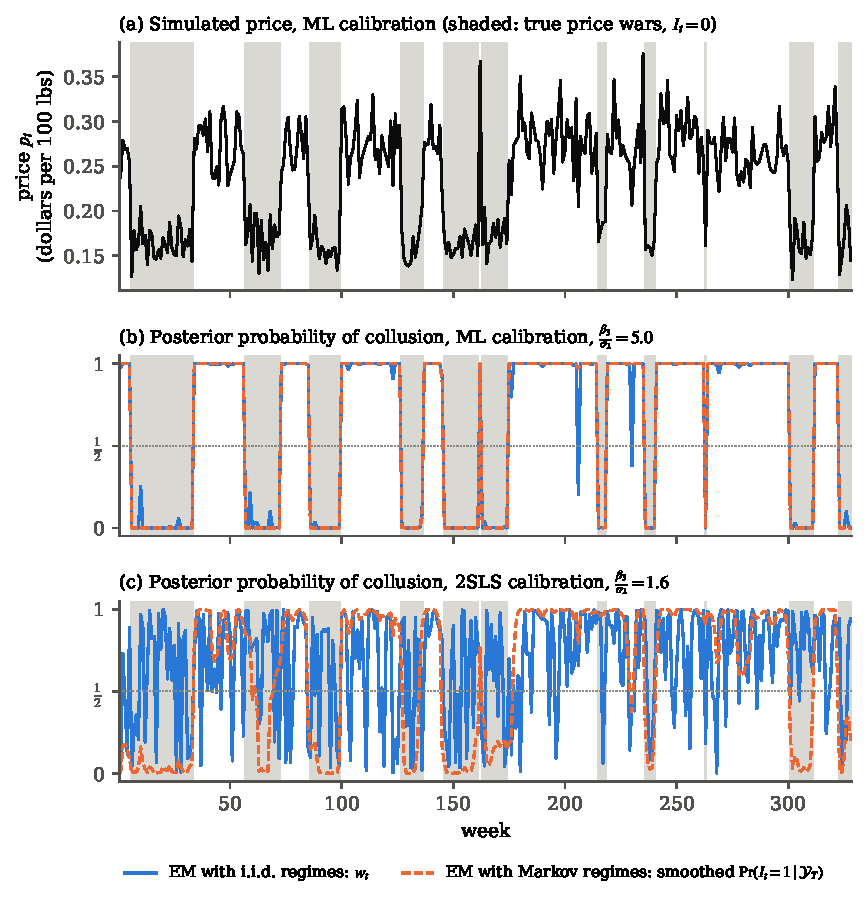
\includegraphics[width=0.92\textwidth]{figures/ch13/regime_sim.pdf}
\caption{A simulated regime-switching price path and the estimated regimes. Panel (a) shows the simulated grain
rate for the calibration to the maximum likelihood column of \citet[Table~3]{Porter1983}, with true price-war
weeks shaded. Panels (b) and (c) show the posterior probability of collusion from EM with i.i.d.\ regimes (solid)
and the smoothed probability from EM with Markov regimes (dashed). Panel (c) uses the two-stage least squares
calibration, in which the regimes are less well separated. Source: our simulation calibrated to Porter (1983,
Tables 3 and 4).}
\label{fig:13-gp-path}
\end{figure}

\begin{figure}[htbp]
\centering
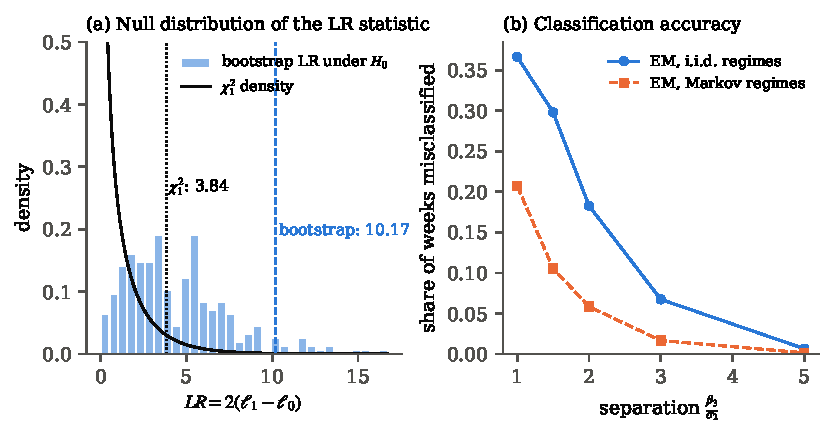
\includegraphics[width=0.95\textwidth]{figures/ch13/em_mc.pdf}
\caption{Panel (a): null distribution of the likelihood-ratio statistic for no switching, from 300 parametric
bootstrap samples of 328 weeks generated without switching, against the $\chi^2_1$ density. The bootstrap 95th
percentile is 10.17, against 3.84 for $\chi^2_1$. Panel (b): average share of misclassified weeks over 60
simulated samples for each separation ratio $\frac{\beta_3}{\sigma_2}$, holding the other parameters at the maximum
likelihood calibration. Source: our simulation.}
\label{fig:13-em-mc}
\end{figure}

The Monte Carlo experiments in \cref{fig:13-em-mc} make the lessons general. Panel (a) shows the null distribution
of the likelihood-ratio statistic for no switching in samples of 328 weeks. Its 90, 95 and 99 percent quantiles are
8.34, 10.17 and 13.17, against 2.71, 3.84 and 6.63 for $\chi^2_1$. A test that used the $\chi^2_1$ cutoff of 3.84
would reject a true null of no switching in 49 percent of samples. Panel (b) shows that classification deteriorates
quickly as separation falls. With i.i.d.\ regimes the share of misclassified weeks is 0.6 percent at a ratio of 5,
6.7 percent at 3, 18 percent at 2 and 37 percent at 1. At a ratio of 1 this is barely better than calling every week
collusive, which errs 38 percent of the time. The Markov model misclassifies 0.1, 1.7, 5.8 and 21 percent. At a ratio
of 1 it even beats the i.i.d.\ Bayes rule with known parameters, whose error is 29 percent, because neighboring weeks
carry information about the regime. The estimated demand slope degrades as well. Across samples, the standard
deviation of $\hat\alpha_1$ from the i.i.d.\ model is 0.09 at a ratio of 5, the same as with known regimes. It is 0.40
at a ratio of 2 and above 1 at lower ratios, while known regimes keep it near 0.09. Porter's maximum likelihood (ML) estimates imply a
ratio of 5.0, so his classification is reliable if his model is right. His 2SLS estimates imply a ratio of 1.6, a
reminder that the separation is itself estimated.

The Berry-Briggs test behaves as the theory predicts on simulated regime series of the same length. On a
first-order Markov chain with the transition probabilities above, the test of $\Pr(I_t = 1\mid 0, 0) =
\Pr(I_t = 1 \mid 1, 0)$, where histories are written $(I_{t-2}, I_{t-1})$, gives $W = 0.34$. On a Green-Porter
chain in which every war lasts exactly 10 weeks, it gives $W = 10.11$. The difference comes from the first week of
a war. Under Green and Porter, a war that has just begun never ends the next week, so $\hat p_{(1,0)} = 0$, while
$\hat p_{(0,0)} = 0.110$ because some wars end after ten weeks. With six to eleven wars in real data, power is low,
and cells with zero variance are common.

\section{The Joint Executive Committee Railroad Cartel}\label{sec:13-jec}

The Joint Executive Committee (JEC) is the most studied cartel in empirical industrial organization. It was legal,
it kept weekly records, and its history includes price wars that contemporaries reported. \Citet{Porter1983} used
its records to estimate the switching model of \cref{sec:13-implications}, and \citet{Ellison1994} re-estimated it
with Markov regimes to ask what started the wars. This section treats both papers in depth.

\subsection{Question and setting}\label{sec:13-jec-setting}

\casehead{The question}
Distinguishing collusion from noncooperative behavior without a smoking gun is hard (p.~301). Porter asks whether
the prices of the JEC switched between collusive and noncooperative regimes, as the trigger-price equilibrium of
\citet{GreenPorter1984} predicts. The alternative is that shifts in demand and cost explain all movements in price
and quantity. The test matters beyond railroads. If wars are part of a collusive equilibrium, an industry with
recurrent price wars is not one in which collusion keeps failing. Green and Porter stress that this undercuts a
common argument against antitrust intervention.

\casehead{The Green-Porter model}
In \citet{GreenPorter1984}, $N$ firms produce a homogeneous good. The market price is
$p_t = \zeta_t\, p\big(\sum_i x_{it}\big)$, where $x_{it}$ is firm $i$'s output and $\zeta_t$ is an i.i.d.\
demand shock with mean one that firms do not observe. Firms see the price but not their rivals' outputs. They produce
collusive quantities while the price stays above a trigger price $\bar p$. When the price falls below $\bar p$, they
produce Cournot quantities for $T - 1$ periods and then resume collusion. In equilibrium no firm cheats, yet wars
occur whenever a low demand shock pushes the price below the trigger. If $F$ is the distribution of $\zeta_t$ and
$y_i$ are the collusive outputs, a war starts in each collusive period with probability
$F(\frac{\bar p}{p(\sum_i y_i)})$. Porter uses three predictions: switches between regimes occur, they follow a pattern, and
collusive output exceeds the static joint-profit level \citep{Porter1983b}.

\casehead{The cartel}
The JEC controlled eastbound freight shipments from Chicago to the Atlantic seaboard. The railroads involved formed
it by agreement in April 1879 and acknowledged it publicly. It preceded the Interstate Commerce Act (1887) and the
Sherman Act (1890), so it was legal (p.~302). According to \citet{Ulen1979}, its enforcement resembled a trigger
strategy. In several instances the cartel thought that cheating had occurred, cut prices for a time, and then
returned to the collusive price.

\casehead{The product}
Grain accounted for 73 percent of the dead-freight tonnage of the JEC, and the rates for flour and provisions were
tied to the grain rate (p.~303). Grain is not perishable, so speed of delivery was not a margin of
differentiation. Most of the wheat was exported, and the rates of different railroads adjusted to compensate for
differences in ocean shipping rates from their port cities. Porter therefore treats the service as a homogeneous
good.

\casehead{Price setting and monitoring}
Railroads set prices, not quantities. Under price setting the natural reversion is Bertrand, which is why the
supply relation of \cref{prop:13-porter-supply} has $\theta = 0$ in wars. The agreement allotted market shares, and
each firm set its rates individually. The JEC office kept weekly accounts, so each railroad saw total shipments.
Actual shares depended on all firms' prices and on unpredictable forces. A firm with a low share could not tell a
rival's secret rate cut from bad luck. This is the inference problem of \citet{Stigler1964}, and it is close to the
Green-Porter problem. \Citet{BrockScheinkman1985} show that equilibria with similar features exist in price-setting
supergames with capacity constraints.

\casehead{Entry and competition}
Entry occurred twice. The Grand Trunk Railway entered in 1880 and the Chicago and Atlantic in 1883. The cartel
accepted the entrants and gave them share allotments. A railroad that entered faced a ``no-exit'' constraint:
bankrupt railroads were relieved by the courts of most of their fixed costs and told to cut prices to raise business
(p.~303). Predation was therefore pointless. Entry shifted the cost constant $A$, and collusion continued.
The main competition came from lake steamers and sailships, which never joined the agreement. The opening and
closing of the Great Lakes to navigation shifted demand predictably, and rates adjusted to the season without
disrupting conduct.

\subsection{Data}\label{sec:13-jec-data}

The data are weekly from week 1 of 1880 to week 16 of 1886, a total of 328 weeks, compiled by \citet{Ulen1979}.
\Cref{tab:13-jec-data} lists the variables and their summary statistics. The price GR is the grain rate in dollars
per 100 pounds and the quantity TQG is total grain shipped by JEC members in tons. LAKES equals one when the Great
Lakes were open to navigation. PO equals one unless the trade magazine \textit{Railway Review} reported a price war,
and it agrees with the reports of the \textit{Chicago Tribune}. PN is the regime classification that Porter
estimates. Four dummies mark changes in the membership of the cartel. Each year is divided into thirteen four-week
periods, and twelve ``monthly'' dummies enter both equations.

\begin{table}[htbp]
\centering
\caption{The JEC data, 1880--1886}\label{tab:13-jec-data}
\small
\begin{tabularx}{\textwidth}{@{}l>{\raggedright\arraybackslash}Xcccc@{}}
\toprule
Variable & Definition & Mean & Std.\ dev. & Min. & Max.\\
\midrule
GR & Grain rate, dollars per 100 lbs & 0.2465 & 0.06653 & 0.125 & 0.40\\
TQG & Total grain shipped, tons per week & 25{,}384 & 11{,}632 & 4{,}810 & 76{,}407\\
LAKES & $=1$ if the Great Lakes were open & 0.5732 & 0.4954 & 0 & 1\\
PO & $=1$ unless a price war was reported & 0.6189 & 0.4864 & 0 & 1\\
DM1 & Grand Trunk entry (week 28, 1880 to week 10, 1883) & 0.4238 & 0.4949 & 0 & 1\\
DM2 & Addition to New York Central (weeks 11--25, 1883) & 0.0457 & 0.2092 & 0 & 1\\
DM3 & Chicago and Atlantic entry (week 26, 1883 to week 11, 1886) & 0.4329 & 0.4962 & 0 & 1\\
DM4 & Chicago and Atlantic leaves (weeks 12--16, 1886) & 0.0152 & 0.1227 & 0 & 1\\
\bottomrule
\end{tabularx}

\smallskip
\begin{minipage}{0.95\textwidth}\footnotesize
Notes: 328 weekly observations. Definitions from \citet[Table~1]{Porter1983}. Statistics for GR, TQG, LAKES and PO
from \citet[Table~2]{Porter1983}, and for DM1--DM4 from \citet[Table~1]{Ellison1994}, which reports the same values
for GR, TQG and LAKES (to fewer digits) but not PO.
\end{minipage}
\end{table}

The dummies cover the sample in five periods. DM1 and DM3 mark the two long periods, 139 and 142 weeks, and together
they cover 281 of the 328 weeks (our computation of the 139 and 142). All price wars occurred inside them (p.~308).

\casehead{Three caveats}
First, the price series is suspect. The JEC polled its members and published an index of their rates. Secret price
cuts would not show up in such an index, because members had no incentive to report them (p.~307). Wars started by
secret cuts may therefore appear in GR with a lag. Porter notes the other side of this coin: an imperfect information
structure is exactly what a trigger-price equilibrium requires. Second, the prices charged by lake steamers, the main
competitors, are not available, so LAKES stands in for them. Third, the model assumes constant market shares across
regimes. Within the DM1 and DM3 periods the average sum of squared deviations from allotted shares was roughly the
same in cooperative and war weeks, which supports the assumption (p.~308). The reported regime series PO also
conflicts sharply with an index of cartel adherence built by \citet{MacAvoy1965}. This conflict is one reason to
estimate the regimes from prices and quantities.

\subsection{Model and estimating equations}\label{sec:13-jec-model}

The estimating equations are demand \eqref{eq:13-demand} and the supply relation \eqref{eq:13-supply-est}, with
twelve seasonal dummies added to both:
\begin{align}
  \log TQG_t &= \alpha_0 + \alpha_1 \log GR_t + \alpha_2 LAKES_t + \text{seasonal dummies} + U_{1t},
  \label{eq:13-porter-demand}\\
  \log GR_t &= \beta_0 + \beta_1 \log TQG_t + \beta_2^\top (DM1_t, \dots, DM4_t)^\top + \beta_3 I_t
  + \text{seasonal dummies} + U_{2t}. \label{eq:13-porter-supply}
\end{align}
The errors are i.i.d.\ bivariate normal with covariance $\Sigma$. By \cref{prop:13-porter-supply}, if wars are
Bertrand reversions, $\beta_0 = \log A$, $\beta_1 = \psi - 1 > 0$ and $\beta_3 > 0$. If cooperative periods
maximized static joint profit, $\beta_3$ would equal $\log\frac{\alpha_1}{1+\alpha_1}$ (\cref{cor:13-static-monopoly}).
Porter leaves $\beta_3$ unrestricted. An optimal trigger-price cartel should set $\beta_3$ positive but below that
level.

Identification follows \cref{sec:13-switching-id}. LAKES shifts demand and identifies the supply slope $\beta_1$.
The regime and the entry dummies shift supply and identify the demand slope $\alpha_1$. Porter estimates the model in
two ways. The first treats PO as the true regime series and applies two-stage least squares. The second treats
$I_t$ as unknown and i.i.d.\ Bernoulli$(\lambda)$, as in \eqref{eq:13-mixture}, and maximizes the likelihood by the
EM algorithm of \cref{sec:13-em}. Weeks with $w_t > \frac{1}{2}$ are classified as collusive (\cref{prop:13-classify}),
which yields PN. Porter acknowledges that a Green-Porter regime series would be Markov of order $T-1$. He gives three
reasons for not imposing it. Estimating under that constraint is hard. The length of wars should vary as entry
changes the cartel's problem. \Citet{GreenPorter1984} show that the bias from treating the regime process as
exogenous is slight when wars are few relative to the sample (pp.~306--307). He also estimated a linear version of the model and found
results that were not significantly different.

\subsection{Results}\label{sec:13-jec-results}

\Cref{tab:13-porter-t3} reproduces Porter's estimates. In the 2SLS columns all coefficients have the expected sign,
but the fit is modest, with a supply $R^2$ of 0.320. In the ML columns the demand equation is practically unchanged.
The supply equation changes. The regime coefficient rises from 0.382 to 0.545 and its standard error halves, while the
supply $R^2$ rises to 0.863 and the standard error of the regression falls from 0.243 to 0.109.

\begin{table}[htbp]
\centering
\caption{Porter's estimates of the JEC demand and supply relations}\label{tab:13-porter-t3}
\small
\begin{tabular}{@{}lcccc@{}}
\toprule
 & \multicolumn{2}{c}{2SLS, regimes from PO} & \multicolumn{2}{c}{ML (EM), regimes estimated}\\
\cmidrule(lr){2-3}\cmidrule(l){4-5}
Variable & Demand & Supply & Demand & Supply\\
\midrule
Constant & 9.169 & $-3.944$ & 9.090 & $-2.416$\\
 & (0.184) & (1.760) & (0.149) & (0.710)\\
LAKES ($\alpha_2$) & $-0.437$ & & $-0.430$ & \\
 & (0.120) & & (0.120) & \\
$\log GR$ ($\alpha_1$) & $-0.742$ & & $-0.800$ & \\
 & (0.121) & & (0.091) & \\
DM1 & & $-0.201$ & & $-0.165$\\
 & & (0.055) & & (0.024)\\
DM2 & & $-0.172$ & & $-0.209$\\
 & & (0.080) & & (0.036)\\
DM3 & & $-0.322$ & & $-0.284$\\
 & & (0.064) & & (0.027)\\
DM4 & & $-0.208$ & & $-0.298$\\
 & & (0.170) & & (0.073)\\
PO or PN ($\beta_3$) & & 0.382 & & 0.545\\
 & & (0.059) & & (0.032)\\
$\log TQG$ ($\beta_1$) & & 0.251 & & 0.090\\
 & & (0.171) & & (0.068)\\
\midrule
$R^2$ & 0.312 & 0.320 & 0.307 & 0.863\\
Std.\ error of regression & 0.398 & 0.243 & 0.399 & 0.109\\
\bottomrule
\end{tabular}

\smallskip
\begin{minipage}{0.9\textwidth}\footnotesize
Notes: From \citet[Table~3]{Porter1983}. Standard errors in parentheses. $T = 328$ weeks. Twelve seasonal dummies
are included in both equations and not reported in the paper. In the ML columns the regime variable is the estimated
classification PN.
\end{minipage}
\end{table}

\casehead{Demand}
Demand is inelastic, with $\hat\alpha_1 = -0.742$ or $-0.800$. Industry marginal revenue
$p(1 + \frac{1}{\alpha_1})$ is then negative. By \cref{cor:13-static-monopoly}, the JEC did not maximize static joint
profit: marginal revenue would have to equal a share-weighted average of marginal costs, which is positive
(p.~308). As expected, open lakes shift rail demand down by 0.43 to 0.44 log points, about 35 percent at a
given price.

\casehead{Supply}
Price is significantly higher in cooperative periods. The supply relation slopes up, which suggests weak
diseconomies of scale, but $\hat\beta_1$ is small and significant only at the 15 percent level in the 2SLS columns.
The entry dummies are negative, and DM3 is below DM2, so each entry lowered the supply intercept. This is the sign
that \cref{prop:13-porter-supply} predicts for an increase in $\Sigma_a$.

\begin{example}[Conduct and margins in cooperative weeks]\label{ex:13-porter-theta}
Apply \eqref{eq:13-theta-from-beta3} to the ML estimates:
\begin{equation*}
  \theta = -0.800\left(e^{-0.545} - 1\right) = -0.800\,(0.580 - 1) = 0.336 .
\end{equation*}
Porter reports this value and calls it roughly consistent with Cournot behavior in cooperative periods (pp.~309--310).
The 2SLS estimates give $\theta = -0.742(e^{-0.382} - 1) = -0.742\,(0.682 - 1) = 0.236$ (our computation). By
\eqref{eq:13-lerner-beta3} the Lerner index in cooperative weeks is $1 - e^{-0.545} = 0.42$ in the ML estimates and
$1 - e^{-0.382} = 0.32$ in the 2SLS estimates (our computation). Porter stresses that the Cournot label has no special
meaning. What matters is that cooperative prices exceed competitive prices but stay below the static joint-profit
level, as an optimal trigger-price cartel would set them.
\end{example}

\begin{example}[Reduced-form effects of collusion and of the lakes]\label{ex:13-porter-rf}
Solve the ML system for the effect of the regime, holding the other variables fixed. Substitute demand into supply:
\begin{equation*}
  \log p = \beta_0' + \beta_1\left(\alpha_0' + \alpha_1\log p + \alpha_2 L\right) + \beta_3 I,
\end{equation*}
where primes denote intercepts that absorb the other variables. Collect the $\log p$ terms:
\begin{equation*}
  (1 - \alpha_1\beta_1)\log p = \beta_0' + \beta_1\alpha_0' + \beta_1\alpha_2 L + \beta_3 I .
\end{equation*}
Hence
\begin{align*}
  \frac{\partial \log p}{\partial I} &= \frac{\beta_3}{1 - \alpha_1\beta_1} = \frac{0.545}{1 + 0.800 \times 0.090}
  = \frac{0.545}{1.072} = 0.508, \\
  \frac{\partial\log Q}{\partial I} &= \alpha_1\frac{\partial\log p}{\partial I} = -0.800\times 0.508 = -0.407 .
\end{align*}
Collusion multiplies price by $e^{0.508} = 1.66$ and quantity by $e^{-0.407} = 0.67$. Revenue rises by the factor
$e^{0.508 - 0.407} = e^{0.101} = 1.11$. For the lakes,
\begin{align*}
  \frac{\partial\log Q}{\partial L} &= \frac{\alpha_2}{1 - \alpha_1\beta_1} = \frac{-0.430}{1.072} = -0.401, \\
  \frac{\partial\log p}{\partial L} &= \frac{\beta_1\alpha_2}{1 - \alpha_1\beta_1} = 0.090 \times (-0.401) = -0.036 .
\end{align*}
Open lakes multiply quantity by $e^{-0.401} = 0.67$ and price by $e^{-0.036} = 0.965$ (our computation throughout).
Because the model is log-linear, these ratios do not depend on where the other variables are held.
\end{example}

\Cref{tab:13-porter-t4} reports Porter's predicted values at the sample means of the other variables. The ratios
match the example. Price is 66 percent higher in cooperative weeks ($\frac{0.2780}{0.1673} = 1.66$), quantity 33
percent lower, and revenue 11 percent higher, a difference of about 11,000 dollars a week in 1880 dollars. These
are Porter's figures (p.~310). The entries of \cref{tab:13-porter-t4} give 13,886 dollars with the lakes closed and
8,970 with them open. Porter's
text says that price was 4.5 percent lower when the lakes were open. The table implies
$\frac{0.1612}{0.1673} = 0.964$, a fall of 3.6 percent, which agrees with the reduced form of
\cref{ex:13-porter-rf}.
Revenue is about 35 percent lower when the lakes are open. Revenue on grain was 70 to 80 percent of the JEC's revenue
from eastbound freight.

\begin{table}[htbp]
\centering
\caption{Predicted price, quantity and revenue by regime and season}\label{tab:13-porter-t4}
\small
\begin{tabular}{@{}lcccc@{}}
\toprule
 & \multicolumn{2}{c}{Lakes closed (LAKES $= 0$)} & \multicolumn{2}{c}{Lakes open (LAKES $= 1$)}\\
\cmidrule(lr){2-3}\cmidrule(l){4-5}
 & War & Cooperation & War & Cooperation\\
 & (PN $= 0$) & (PN $= 1$) & (PN $= 0$) & (PN $= 1$)\\
\midrule
Price (GR, dollars per 100 lbs) & 0.1673 & 0.2780 & 0.1612 & 0.2679\\
Quantity (TQG, tons per week) & 38{,}680 & 25{,}775 & 25{,}904 & 17{,}261\\
Revenue (dollars per week) & 129{,}423 & 143{,}309 & 83{,}514 & 92{,}484\\
\bottomrule
\end{tabular}

\smallskip
\begin{minipage}{0.95\textwidth}\footnotesize
Notes: From \citet[Table~4]{Porter1983}. Computed from the reduced form of the ML estimates in
\cref{tab:13-porter-t3}, with the other explanatory variables at their sample means. Revenue is
$20 \times \text{GR} \times \text{TQG}$: a ton is 20 hundredweight, so this converts dollars per 100 pounds times tons
into dollars.
\end{minipage}
\end{table}

\casehead{Timing of the wars}
\Cref{fig:13-porter-f1} plots the grain rate with the weeks in which PO and PN indicate a war. The two series agree
broadly. Wars averaged about 10 weeks and occurred mainly in 1881, 1884 and 1885. In several episodes PO records a
war before PN does, and the two return to cooperation together (p.~310). This pattern fits a price index that
misses secret cuts at the start of a war. PN was not constrained to resemble PO in any way. \Cref{tab:13-porter-t5}
shows that it agrees with the trade-press reports and disagrees with MacAvoy's index of share instability. MacAvoy's index is
highest in 1880, a year without any war in either PO or PN.

\begin{figure}[htbp]
\centering
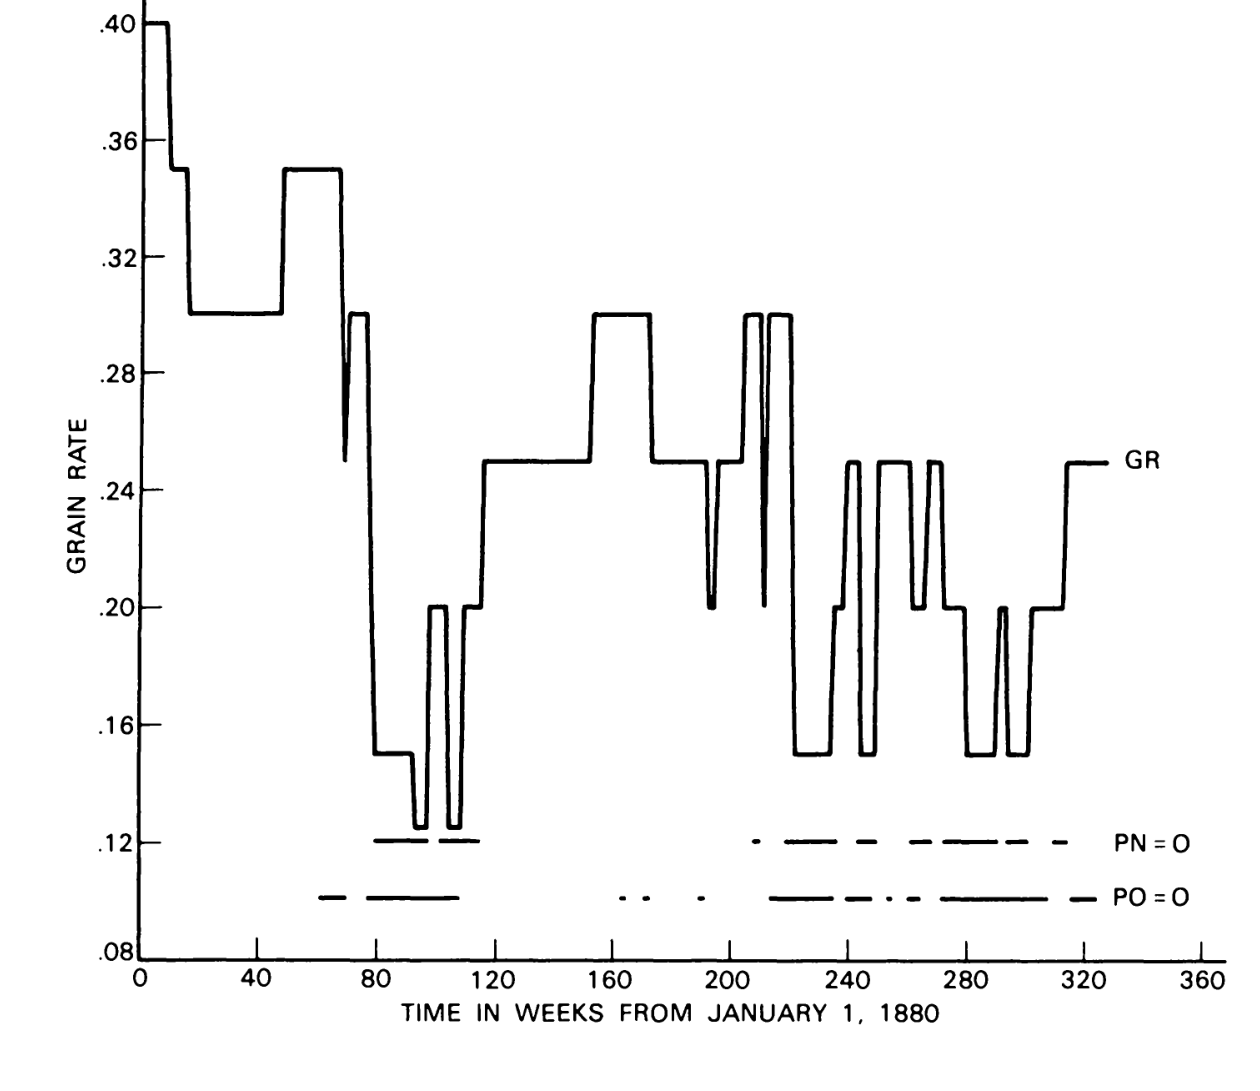
\includegraphics[width=0.78\textwidth]{figures/ch13/porter1983_fig1.png}
\caption{The JEC grain rate in dollars per 100 pounds, from January 1880. Upper segments mark the weeks that the
estimated series classifies as price wars (PN $= 0$), and lower segments those of the trade-press series
(PO $= 0$). Source: Porter (1983), Figure 1.}
\label{fig:13-porter-f1}
\end{figure}

\begin{table}[htbp]
\centering
\caption{Indices of cartel nonadherence by year}\label{tab:13-porter-t5}
\small
\begin{tabular}{@{}lccc@{}}
\toprule
 & & \multicolumn{2}{c}{Share of weeks at war}\\
\cmidrule(l){3-4}
Year & MacAvoy's index & Reported (PO) & Estimated (PN)\\
\midrule
1880 & 26 & 0.00 & 0.00\\
1881 & 14 & 0.67 & 0.44\\
1882 & 18 & 0.06 & 0.21\\
1883 & 6 & 0.10 & 0.00\\
1884 & 16 & 0.58 & 0.40\\
1885 & 10 & 0.77 & 0.67\\
1886 (16 weeks) & 15 & 0.50 & 0.06\\
\bottomrule
\end{tabular}

\smallskip
\begin{minipage}{0.95\textwidth}\footnotesize
Notes: From \citet[Table~5]{Porter1983}, whose first two columns come from \citet{Ulen1979}. MacAvoy's index counts
months, summed over members, in which a member's share of tonnage deviated from its trend share. A deviation counts
when it exceeds the standard error of the member's trend regression. The reported and estimated columns are
$\frac{1}{52}\sum_t(1 - PO_t)$ and $\frac{1}{52}\sum_t(1 - \hat I_t)$ over the weeks of each year, with denominator 16
in 1886.
\end{minipage}
\end{table}

\casehead{Testing for switching}
The coefficients on PO and PN are significantly positive, so cooperative periods had significantly higher prices.
Porter's likelihood-ratio statistic \eqref{eq:13-porter-lr} is $2T(L_1 - L_0) = 554.1$. He refers it to the
$\chi^2_1$ distribution and rejects the hypothesis of no switching overwhelmingly. As \cref{sec:13-tests} explains,
the $\chi^2_1$ reference is invalid, and the statistic omits the mixing terms of the likelihood. Its simulated null
distribution, with a 95th percentile near 240 in our calibration, still lies far below 554. Price and quantity
changes cannot be attributed to demand and structural shifts alone, given the specification. The agreement between
PN and PO also shows that the estimated switches are not an artifact of missing data.

\casehead{Entry and the frequency of wars}
The 1881 and 1884 wars each began about 40 weeks after an entry, of the Grand Trunk and of the Chicago and Atlantic
respectively (p.~311). Entry did not cause an immediate reversion. It plausibly raised the chance of later
ones. Wars were more frequent, and shorter on average, when the cartel had more members. This fits the general
point that enforcement gets harder as the number of firms grows (\cref{ch:collusion-theory}).

\casehead{Triggers}
Green-Porter wars follow unexpected demand drops. Porter regresses the length of each war on the demand residual in
the week before it began and finds little predictive power. Price wars were not preceded by large negative demand
residuals. He offers two reasons for caution. The demand residual omits the lake steamers' prices, so it measures
unexpected demand poorly. The firms set prices, so wars may have followed unpredictable swings in market shares, as
\citet{Stigler1964} predicts.

\Cref{tab:13-porter-t6} gives annual wheat shipments from Chicago by lake and by rail. 1880 was a boom year, which
accounts for its high rates. Among the other years, total shipments are not correlated with nonadherence. The war
years 1881, 1884 and 1885 stand out by the JEC's high share of intermodal shipments: 50.0, 34.0 and 48.5 percent,
against 13.8 to 26.8 percent in 1882, 1883 and 1886. JEC wars did not coincide with lake steamer price wars, and they
did not always occur when total demand was low. They were not systematically related to the opening or closing of the
lakes either (p.~313).

\begin{table}[htbp]
\centering
\caption{Annual eastbound shipments of wheat from Chicago by lake and rail}\label{tab:13-porter-t6}
\small
\begin{tabular}{@{}lccccc@{}}
\toprule
 & \multicolumn{2}{c}{Lake} & \multicolumn{2}{c}{Rail} & Total\\
\cmidrule(lr){2-3}\cmidrule(lr){4-5}
Year & Millions of bushels & Percent & Millions of bushels & Percent & millions of bushels\\
\midrule
1880 & 16.69 & 77.9 & 4.728 & 22.1 & 21.42\\
1881 & 7.688 & 50.0 & 7.680 & 50.0 & 15.37\\
1882 & 14.94 & 86.2 & 2.389 & 13.8 & 17.33\\
1883 & 7.067 & 73.2 & 2.590 & 26.8 & 9.66\\
1884 & 11.52 & 66.0 & 5.928 & 34.0 & 17.45\\
1885 & 5.436 & 51.5 & 5.116 & 48.5 & 10.55\\
1886 & 10.51 & 82.6 & 2.209 & 17.4 & 12.72\\
\bottomrule
\end{tabular}

\smallskip
\begin{minipage}{0.75\textwidth}\footnotesize
Notes: From \citet[Table~6]{Porter1983}.
\end{minipage}
\end{table}

\subsection{Ellison's re-examination}\label{sec:13-ellison}

\casehead{The question}
Porter's evidence shows that wars occurred. \Citet[p.~38]{Ellison1994} argues that the core content of the
Green-Porter theory is more specific: wars occur because firms follow strategies in which random demand shocks
trigger them. He asks three questions. Did the wars of the JEC start after the signals that trigger strategies would
use? Were prices less collusive, or wars more likely, in booms, as Rotemberg and Saloner's logic suggests? Did
members cut prices in secret, which no theory of optimal collusion allows?

\casehead{Adapting the theories}
The JEC differs from the textbook Green-Porter model in two ways (pp.~38--39). The railroads set prices, and
reputations for service and different route structures differentiated their demands. Secret cuts made prices
unobservable. The quantity data, in contrast, were presumably reliable. The cartel even considered using the shipment
data to compute side payments by firms that exceeded their allotments. Many trigger strategies could support a
nearly optimal outcome in this setting. Ellison lists three plausible triggers. One firm obtaining a suspiciously high
market share is the best signal of cheating. High aggregate demand is another, because a price cut expands demand as
well as moving shares. An unusually low share for one firm is a third, which a coalition-proof equilibrium might use.

\casehead{Model and data}
Ellison's model follows Porter's closely. Demand is
\begin{equation}\label{eq:13-ellison-demand}
  \log Q_t = \alpha_0 + \alpha_1\log P_t + \alpha_2 LAKES_t + \sum_{k=1}^{12}\alpha_{2+k}\,SEAS_{kt} + U_{1t},
  \qquad U_{1t} = \rho U_{1,t-1} + V_{1t},
\end{equation}
with $|\rho| < 1$. The supply relation is
\begin{equation}\label{eq:13-ellison-supply}
  \log P_t = \beta_0 + \beta_1\log Q_t + \beta_3 I_t + \sum_{k=1}^{4}\beta_{3+k}\,DM_{kt} + U_{2t},
\end{equation}
where we keep our $\beta_3$ for the coefficient that Ellison writes $\beta_2$. The errors $(V_{1t}, U_{2t})$ are
bivariate normal. Regimes follow the logit Markov chain \eqref{eq:13-logit-transition}, with
\begin{equation}\label{eq:13-ellison-logit}
  \Pr(I_{t+1} = 1 \mid I_t, Z_t) = \Lambda\left(\gamma_1 I_t + \gamma_0(1 - I_t) + \gamma_Z^\top Z_t I_t\right),
\end{equation}
where $Z_t$ holds candidate triggers. A negative element of $\gamma_Z$ means that the variable raises the probability
that a collusive week is followed by a war. The structural equations and the transitions are estimated jointly by
maximum likelihood with the filter of \cref{sec:13-markov}, following \citet{CosslettLee1985}. Standard errors are
robust and computed from numerical derivatives. Joint estimation should date the onset of wars more accurately than
Porter's two-step approach and give more power to detect triggers. The data are Ulen's weekly series, the same 328
weeks that Porter used.

\Cref{fig:13-ellison-regimes} summarizes the regime structures that Ellison estimates, including the hidden demand
regimes introduced below.

\begin{figure}[htbp]
\centering
\begin{tikzpicture}[>=Stealth, font=\footnotesize,
  box/.style={draw, rounded corners=2pt, align=center, minimum width=4.2cm, inner sep=3pt, fill=white}]
  \draw[rounded corners=6pt, thick] (-2.4,-2.75) rectangle (2.4,2.35);
  \node[font=\small] at (0,1.95) {Collusion, $I_t = 1$};
  \node[box] at (0,1.0) {REGIME1: high demand\\ probability $r_1$};
  \node[box] at (0,-0.35) {REGIME2: medium demand\\ probability $r_2$};
  \node[box] at (0,-1.85) {REGIME3: low demand\\ probability $1 - r_1 - r_2$};
  \draw[rounded corners=6pt, thick] (5.6,-2.45) rectangle (10.4,1.85);
  \node[font=\small] at (8.0,1.45) {Price war, $I_t = 0$};
  \node[box] at (8.0,0.4) {REGIME2: medium demand\\ probability $\frac{r_2}{1 - r_1}$};
  \node[box] at (8.0,-1.3) {REGIME3: low demand\\ probability $\frac{1 - r_1 - r_2}{1 - r_1}$};
  \draw[->, thick] (2.4,0.55) -- node[above, align=center] {$q_{10,t} = 1 - q_{11,t}$} (5.6,0.55);
  \draw[->, thick] (5.6,-1.0) -- node[below, align=center] {$q_{01,t} = \Lambda(\gamma_0)$} (2.4,-1.0);
  \draw[->, thick] (-0.9,2.35) .. controls (-1.2,3.5) and (1.2,3.5) .. (0.9,2.35);
  \node at (0,3.7) {$q_{11,t} = \Lambda(\gamma_1 + \gamma_Z^\top Z_t)$};
  \draw[->, thick] (7.1,1.85) .. controls (6.8,3.0) and (9.2,3.0) .. (8.9,1.85);
  \node at (8.0,3.2) {$q_{00,t} = 1 - q_{01,t}$};
\end{tikzpicture}
\caption{The regime structure in \citet{Ellison1994}. Conduct follows a two-state Markov chain whose transition
probabilities are logits. Candidate triggers $Z_t$ enter only the probability $q_{11,t}$ of staying in collusion.
In the hidden-regime models, demand regimes are drawn each week given conduct. REGIME1 occurs only under collusion,
and the other regimes keep the same relative probabilities in both conduct states. The standard model has no demand
regimes, and model 2 has only REGIME1 and REGIME2. Drawn by us after Ellison's Figures 1 and 3.}
\label{fig:13-ellison-regimes}
\end{figure}

\casehead{The standard model}
\Cref{tab:13-ellison-t2} reports Ellison's ``standard'' model, which adds AR(1) demand errors and Markov regimes to
Porter's specification, next to a version without serial correlation. The lagged demand error has coefficient
$\hat\rho = 0.832$ (0.085), and allowing for it changes the demand estimates. The price elasticity rises from 0.84 to
1.80, so the JEC faced elastic demand. The regime effect hardly moves, from 0.660 to 0.637. By
\eqref{eq:13-theta-from-beta3}, the conduct index rises with the elasticity,
\begin{equation*}
  \theta = 0.843\left(1 - e^{-0.660}\right) = 0.41, \qquad \theta = 1.802\left(1 - e^{-0.637}\right) = 0.85
\end{equation*}
(our computation, against Ellison's reported 0.40 and 0.85). \Cref{rem:13-lerner-vs-theta} explains the pattern. The collusive
Lerner index $1 - e^{-\beta_3}$ is 0.48 or 0.47 in the two columns, and the elasticity converts the same margin into
very different conduct. With elastic demand a static monopoly benchmark exists. \Cref{cor:13-static-monopoly} gives
$\log\frac{1.802}{0.802} = 0.81$, above the estimated 0.637, so the JEC still priced below static monopoly (our
computation). Ellison concludes that the JEC was much more aggressive in its pricing than earlier work reported.

\begin{table}[htbp]
\centering
\caption{Ellison's standard model of the JEC}\label{tab:13-ellison-t2}
\small
\begin{tabular}{@{}lcc@{}}
\toprule
Variable & Standard model & No serial correlation\\
\midrule
\multicolumn{3}{@{}l}{\textit{Demand}}\\
Constant & 7.677 (1.882) & 9.019 (0.361)\\
$\log P$ ($\alpha_1$) & $-1.802$ (1.287) & $-0.843$ (0.193)\\
LAKES & $-0.009$ (0.112) & $-0.460$ (0.348)\\
\multicolumn{3}{@{}l}{\textit{Supply}}\\
Constant & $-4.764$ (1.863) & $-5.649$ (9.461)\\
$\log Q$ ($\beta_1$) & 0.306 (0.178) & 0.398 (0.928)\\
DM1 & $-0.154$ (0.075) & $-0.211$ (0.124)\\
DM2 & $-0.246$ (0.064) & $-0.283$ (0.160)\\
DM3 & $-0.317$ (0.076) & $-0.373$ (0.242)\\
DM4 & $-0.198$ (0.119) & $-0.419$ (0.422)\\
$I_t$ ($\beta_3$) & 0.637 (0.104) & 0.660 (0.406)\\
\multicolumn{3}{@{}l}{\textit{Regimes (logit index)}}\\
Constant if $I_t = 1$ ($\gamma_1$) & 3.675 (0.474) & 3.661 (0.513)\\
Constant if $I_t = 0$ ($\gamma_0$) & $-2.641$ (0.404) & $-2.620$ (0.476)\\
\multicolumn{3}{@{}l}{\textit{Other}}\\
$\sigma_1$ & 0.290 (0.061) & 0.396 (0.029)\\
$\sigma_{12}$ & $-0.007$ (0.004) & $-0.045$ (0.142)\\
$\sigma_2$ & 0.160 (0.045) & 0.191 (0.313)\\
$U_{1,t-1}$ ($\rho$) & 0.832 (0.085) & \\
\midrule
Log likelihood & 181.0 & 37.2\\
\bottomrule
\end{tabular}

\smallskip
\begin{minipage}{0.8\textwidth}\footnotesize
Notes: From \citet[Table~2]{Ellison1994}. Standard errors in parentheses. Twelve seasonal dummies in demand are
included and not shown. The regime constants are the logit indices of $\Pr(I_{t+1} = 1 \mid I_t)$.
\end{minipage}
\end{table}

The regime constants imply strong persistence. The probability that collusion continues is
$\Lambda(3.675) = \frac{e^{3.675}}{1 + e^{3.675}} = 0.975$, and the probability that a war week is followed by
collusion is $\Lambda(-2.641) = 0.067$ (p.~42). By \cref{lem:13-durations}, collusive spells last
$\frac{1}{1 - 0.975} = 40$ weeks on average and wars $\frac{1}{0.067} = 15$ weeks. The long-run share of collusive
weeks is $\frac{0.067}{0.025 + 0.067} = 0.73$ (our computation). The regimes are far from independent, which
confirms the observation of \citet{CosslettLee1985}.

\casehead{Candidate triggers}
To test for triggers, Ellison builds four share variables (p.~41). Let $s_{it}$ measure the strength of firm $i$'s
demand, and let $\hat s_{it}$ be its predicted value. Each variable is the largest normalized deviation across
firms, $\max_i \frac{s_{it} - \hat s_{it}}{\sigma_i}$, where $\sigma_i$ is the sample standard deviation.
\begin{itemize}
\item \textit{BIGSHARE1} uses $s_{it} = \log q_{it} - \frac{1}{N}\sum_j \log q_{jt}$, where $N$ is the number of
firms, with the average of the
previous twelve weeks as $\hat s_{it}$. Using logs keeps the trade-off between the gain from a price cut and the
loss from a war proportional across firms of different sizes.
\item \textit{BIGSHARE2} uses the ordinary market share, with the same prediction.
\item \textit{BIGSHAREQ} uses the log measure, with the assigned quota as the prediction. Quotas were often set
unrealistically, so deviations from them measure adherence poorly. \citet{MacAvoy1965} reports that the Chicago and
Grand Trunk was admitted with a 10 percent quota while receiving only 2 to 7 percent of the traffic at the cartel
price.
\item \textit{SMALLSHARE} is the largest shortfall of any firm's log measure below its prediction.
\end{itemize}
The demand innovation $V_{1t}$ and the full demand shock $U_{1t}$ serve as aggregate triggers. Under Green and
Porter, unanticipated shocks start wars. Under Rotemberg and Saloner, wars are more likely when demand is high and
expected to decline. Since $U_{1t} = \rho U_{1,t-1} + V_{1t}$, the two can be separated.

\Cref{tab:13-ellison-t3} reports the trigger coefficients. Only six wars are identified in the standard model, so
high significance levels are not to be expected. BIGSHARE1 has the predicted negative sign and is significant at the
6 percent level in a one-tailed test. BIGSHARE2 and BIGSHAREQ are negative but smaller and insignificant.
SMALLSHARE has the wrong sign. The aggregate innovation $V_{1t}$ is large, negative and significant at the 6 percent
level. In model 6 the innovation keeps its sign while the full shock $U_{1t}$ enters with a positive, insignificant
coefficient. The unanticipated component of demand predicts wars and the anticipated component does not. This
separates the Green-Porter explanation from the Rotemberg-Saloner one, which \citet{Porter1985} could not do with a
two-step approach.

\begin{table}[htbp]
\centering
\caption{What started the price wars of the JEC?}\label{tab:13-ellison-t3}
\small
\begin{tabular}{@{}lcccccc@{}}
\toprule
\multicolumn{7}{@{}l}{\textit{Panel A. Estimated regimes, Markov model (Table 3)}}\\
Model & 1 & 2 & 3 & 4 & 5 & 6\\
\midrule
Constant & 4.63 (0.77) & 4.36 (0.77) & 3.95 (1.30) & 2.96 (0.66) & 4.43 (0.81) & 4.35 (0.90)\\
BIGSHARE1 & $-0.77$ (0.49) & & & & & \\
BIGSHARE2 & & $-0.46$ (0.39) & & & & \\
BIGSHAREQ & & & $-0.21$ (1.06) & & & \\
SMALLSHARE & & & & 0.66 (0.89) & & \\
$V_{1t}$ & & & & & $-4.15$ (2.64) & $-5.00$ (3.15)\\
$U_{1t}$ & & & & & & 1.17 (1.15)\\
\midrule
\multicolumn{7}{@{}l}{\textit{Panel B. Reported regimes, logit for the onset of a war (Table 4)}}\\
Model & 1 & 2 & 3 & 4 & & \\
\midrule
Constant & 3.68 (0.65) & 3.55 (0.65) & 3.25 (0.61) & 2.92 (0.57) & & \\
BIGSHARE1 & $-0.71$ (0.46) & & & & & \\
BIGSHARE2 & & $-0.51$ (0.39) & & & & \\
BIGSHAREQ & & & $-0.33$ (0.44) & & & \\
SMALLSHARE & & & & 0.05 (0.37) & & \\
\bottomrule
\end{tabular}

\smallskip
\begin{minipage}{0.95\textwidth}\footnotesize
Notes: From \citet[Tables~3 and 4]{Ellison1994}. Standard errors in parentheses. Coefficients of the logit for
$\Pr(I_{t+1} = 1 \mid I_t = 1, Z_t)$, so a negative coefficient raises the probability that a war begins. In Panel A
each model contains all variables of the standard model. Panel B uses Ulen's reported regimes $J_t$. Means of
BIGSHARE1, BIGSHARE2, BIGSHAREQ and SMALLSHARE are 1.09, 1.24, 1.17 and 1.23 \citep[Table~1]{Ellison1994}.
\end{minipage}
\end{table}

The timing of the estimated wars is uncertain, and the standard model does not match the onset date of Ulen's
classification for any war (p.~43). Panel B of \cref{tab:13-ellison-t3} therefore fits simple logits for the onset
of a war in the reported regime series. The estimates are similar to Panel A, which supports a Green-Porter-type
trigger.

\casehead{Strength of the trigger}
A trigger must also deter cheating. Ellison gives a rough calculation (p.~44). Suppose a firm offers a small secret
price cut that raises its demand by 10 percent and its current profit by 8 to 10 percent. The cut raises its
BIGSHARE1 measure by $\frac{\log 1.1}{\sigma_i}$ when it would otherwise have had the largest deviation. With the
estimated coefficient, a simulation gives an increase in the probability of a war of about 0.001. If a war costs
about 15 times the per-period profit, the expected future loss is about $0.001 \times 15$, roughly 1 to 2 percent of
current profit. The estimated trigger is several times too weak to deter cheating, and the precision of the estimates
does not allow it to be much stronger. Ellison offers two readings. The firms may have reacted to information that
the data miss, or to a true trigger that is only correlated with BIGSHARE1. Alternatively, the JEC's responses may
have been too weak to sustain a noncooperative equilibrium.

\casehead{Booms}
The basic Rotemberg-Saloner model has perfect information and no regime shifts. It is a model of countercyclical
collusion. With imperfect monitoring, its logic implies that a cartel facing a temporary peak in demand lowers its
price or makes its trigger more sensitive (p.~45). A boom here is a period in which current demand is high
relative to demand over the next fifteen weeks or so, the horizon of a war. Two sources create booms in the JEC data.
Serially correlated shocks make a high shock raise demand today by more than in the future. Seasonality makes demand
peak in winter, just before the lakes open. Ellison builds an index of the ratio of current demand to expected
demand during a subsequent war (p.~46),
\begin{equation}\label{eq:13-ellison-boom}
  BOOM_t = K\,\frac{\exp\left(\alpha_2 LAKES_t + \sum_k \alpha_{2+k} SEAS_{kt} + \rho U_{1,t-1}\right)}
  {\sum_{s=1}^{52}\left(\hat p_{w,t+s} - \hat p_{c,t+s}\right)
   \exp\left(\alpha_2 LAKES_{t+s} + \sum_k \alpha_{2+k} SEAS_{k,t+s} + \rho^{s+1}U_{1,t-1}\right)} - 1 .
\end{equation}
Here $\hat p_{w,t+s} - \hat p_{c,t+s}$ is the additional probability of being in a war $s$ weeks after one begins,
taken from the standard model. $K$ is a scaling constant. He adds $BOOM_t I_t$ to the supply relation and
$BOOM_t$ to the transition logit. A seasonal-only version and the lagged shock $U_{1,t-1}$ separate the two sources.

The results are imprecise (\cref{tab:13-ellison-booms}). The coefficient on $BOOM_t I_t$ implies a collusive price
about 3 percent lower when the incentive to deviate is one standard deviation above its mean. Its standard error is
almost twice the estimate, so neither procyclical collusion nor a 12 percent reduction can be rejected (p.~47).
The demand-shock decomposition is more precise but still insignificant. It implies a 5 percent lower price when
$U_{1,t-1}$ is one standard deviation above its mean. The seasonal decomposition shows nothing. In the transition
logit, $BOOM_t$ has the wrong sign. Controlling for the innovation $V_{1t}$, the predictable decline in demand after
a positive shock does not cause wars. The seasonal effect has the right sign but is insignificant.

\begin{table}[htbp]
\centering
\caption{Booms and collusion in the JEC}\label{tab:13-ellison-booms}
\small
\begin{tabular}{@{}lccc@{}}
\toprule
\multicolumn{4}{@{}l}{\textit{Panel A. Supply relation with boom interactions (Table 5)}}\\
 & Combined effect & Demand shocks & Seasonal\\
\midrule
$I_t$ & 0.758 (0.416) & 0.712 (0.195) & 0.622 (0.119)\\
$BOOM_t \times I_t$ & $-0.233$ (0.428) & & \\
$U_{1,t-1}\times I_t$ & & $-0.156$ (0.164) & \\
$SEAS_t \times I_t$ & & & 0.041 (0.417)\\
$\log P$ in demand & $-1.996$ (2.055) & $-1.594$ (0.898) & $-1.574$ (1.459)\\
Log likelihood & 186.2 & 187.1 & 181.2\\
\midrule
\multicolumn{4}{@{}l}{\textit{Panel B. Logit for $\Pr(I_{t+1} = 1\mid I_t = 1, Z_t)$ (Table 6)}}\\
 & Model 1 & Model 2 & Model 3\\
\midrule
Constant & 3.64 (0.49) & 4.35 (0.90) & 3.87 (0.71)\\
$BOOM_t$ & 0.36 (1.48) & & \\
$U_{1t}$ & & 1.17 (1.15) & \\
$V_{1t}$ & & $-5.00$ (3.15) & \\
$SEASONAL_t$ & & & $-2.51$ (3.50)\\
\bottomrule
\end{tabular}

\smallskip
\begin{minipage}{0.9\textwidth}\footnotesize
Notes: From \citet[Tables~5 and 6]{Ellison1994}. Standard errors in parentheses. Rotemberg and Saloner predict a
negative coefficient on the boom interactions in Panel A and negative coefficients on the boom measures in Panel B.
Panel A models also include boom terms in the transition logit. Model 2 of Panel B repeats model 6 of
\cref{tab:13-ellison-t3}.
\end{minipage}
\end{table}

Ellison's verdict is cautious. The JEC does not support the view that wars occur during booms. The tests have little
power, so a small degree of countercyclical pricing or a small rise in the frequency of wars cannot be ruled out. He
also notes that a nineteenth-century railroad cartel is perhaps among the least likely places to apply the theory.

\casehead{Secret price cuts}
All the theories predict that members never cut prices in secret. The trade press of the time suggests that some did.
The \textit{Daily Commercial Bulletin} of June 16, 1881, for example, reported doubts that a quoted rate on grain to
New York was being respected (p.~49). A one-week secret cut would be invisible to an econometrician, as to the
JEC itself. If cutting and adherence were both common, however, secret cuts act like an omitted variable that shifts
demand upward relative to the official price. Ellison looks for such shifts with hidden demand regimes.

Model 2 adds a dummy REGIME1 to demand \eqref{eq:13-ellison-demand}. The high-demand regime occurs with probability
$r_1$ in collusive weeks and never in wars, when firms already price competitively. Model 3 adds two dummies, REGIME1
and REGIME2, for three demand regimes. Under collusion they occur with probabilities $r_1$, $r_2$ and $1 - r_1 - r_2$.
REGIME1 never occurs in wars, and the other two keep their relative probabilities in both conduct states
(\cref{fig:13-ellison-regimes}). Ellison writes $p_1$ and $p_2$ for our $r_1$ and $r_2$. The low regime might reflect
bad weather, labor problems or low steamship rates. Since the regimes enter demand, whose error is autocorrelated, the
filter runs on pairs of consecutive states (\cref{rem:13-ar1}).

\Cref{tab:13-ellison-t7} reports the estimates. Ellison calls the fit almost unreasonably successful. The log
likelihood rises from 181.0 to 529.0 and 582.5. Ellison likens the gain to Porter's when he added a second supply
regime (p.~51). The comparison is loose, because Porter's figure is not a mixture log likelihood
(\cref{sec:13-tests}). The $t$-statistics on REGIME1 are 12.1 and 26.7. In model 2, REGIME1 raises demand by about 55 percent
($e^{0.439} = 1.55$). In model 3, REGIME1 has demand 41 percent above REGIME2, and the low regime has demand 32 percent
below REGIME2 ($e^{0.344} = 1.41$ and $e^{-0.384} = 0.68$).

\begin{table}[htbp]
\centering
\caption{Hidden demand regimes in the JEC}\label{tab:13-ellison-t7}
\small
\begin{tabular}{@{}lccc@{}}
\toprule
 & Model 2 & Model 3 & Model 3 with trigger test\\
 & (Table 7) & (Table 7) & (Table 9)\\
\midrule
\multicolumn{4}{@{}l}{\textit{Demand}}\\
$\log P$ ($\alpha_1$) & $-1.354$ (0.711) & $-1.587$ (0.092) & $-1.57$ (0.43)\\
LAKES & $-0.222$ (0.073) & $-0.229$ (0.092) & $-0.23$ (0.06)\\
REGIME1 & 0.439 (0.036) & 0.728 (0.027) & 0.73 (0.04)\\
REGIME2 & & 0.384 (0.022) & 0.38 (0.05)\\
\multicolumn{4}{@{}l}{\textit{Supply}}\\
$\log Q$ ($\beta_1$) & 0.220 (0.153) & 0.242 (0.038) & 0.24 (0.09)\\
$I_t$ ($\beta_3$) & 0.595 (0.079) & 0.608 (0.047) & 0.61 (0.07)\\
\multicolumn{4}{@{}l}{\textit{Transitions and regime probabilities}}\\
Collusion continues & 0.979 (0.012) & 0.976 (0.037) & logit below\\
War ends & 0.061 (0.028) & 0.070 (0.076) & 0.07 (0.03)\\
$r_1$ & 0.650 (0.071) & 0.256 (0.083) & 0.26 (0.05)\\
$r_2$ & & 0.519 (0.086) & 0.52 (0.07)\\
\multicolumn{4}{@{}l}{\textit{Logit for collusion continuing}}\\
Constant & & & 5.65 (1.06)\\
$V_{1t}$ & & & $-3.17$ (1.26)\\
$RSHIFT_t$ & & & $-0.48$ (1.03)\\
\multicolumn{4}{@{}l}{\textit{Other}}\\
$U_{1,t-1}$ ($\rho$) & 0.888 (0.031) & 0.947 (0.018) & 0.947 (0.02)\\
\midrule
Log likelihood & 529.0 & 582.5 & 584.4\\
\bottomrule
\end{tabular}

\smallskip
\begin{minipage}{0.92\textwidth}\footnotesize
Notes: From \citet[Tables~7 and 9]{Ellison1994}. Standard errors in parentheses. Seasonal dummies, the constants, the
entry dummies and the error covariances are included and not shown. ``Collusion continues'' and ``war ends'' are
Ellison's $q_{123}$ (or $q_{12}$) and $q_0$. $RSHIFT_t = \alpha_{15}REGIME1_t + \alpha_{16}(REGIME2_t - 1)$ is the
demand effect of the hidden regimes. Table 9 reports two decimals.
\end{minipage}
\end{table}

\casehead{Interpreting the hidden regimes}
Ellison warns that the regimes could reflect weather, irregular schedules, steamship competition, mechanical
problems, or failures of the functional form (p.~52). He checks three kinds of evidence.

The first is the size and frequency of the implied cuts. Trade-press reports suggest that cuts of 10 to 25 percent
were reasonable, and the cartel sometimes went two years between wars, so cuts were not very common (p.~53). In
model 2, REGIME1 occurs in 65 percent of collusive weeks, and with an elasticity of 1.35 it would require price cuts
of 25 to 30 percent. Ellison rejects it as a measure of secret cuts. In model 3, REGIME1 occurs in 26 percent of
collusive weeks, and with an elasticity of 1.59 it requires a cut of about 20 percent. To check, solve
$(1 - x)^{-1.587} = e^{0.344}$ for the cut $x$:
\begin{equation*}
  x = 1 - \exp\left(-\frac{0.344}{1.587}\right) = 1 - e^{-0.217} = 0.195
\end{equation*}
(our computation). A kernel density of the standard model's demand residuals $\hat V_{1t}$ has a second, smaller peak
to the right, as occasional price cuts of similar size would produce \citep[Figure~2]{Ellison1994}.

The second is historical evidence on cutting. Ellison codes two indicators from the \textit{Daily Commercial
Bulletin}. CUTREPORTED marks the 12 weeks in which an article reported rumors of secret cuts. CUTLISTED marks the 18
weeks in which the average listed daily price was at least three cents below the official price. Overall, 26 percent
of weeks fall in the high-demand regime. One and two weeks after a CUTREPORTED week, the shares are 57 and 66 percent,
both significantly higher (Table~8, p.~54). Four weeks after a CUTLISTED week the share is 60 percent, and after a
reported war it is 40 to 46 percent at lags of two to four weeks. The pattern fits retaliatory cutting after reports of
cheating. About 15 percent of high-demand weeks are attributable to these excess occurrences.

The third is a test of observability. If the hidden regimes were invisible to the JEC, a Green-Porter trigger would
respond to total unexpected demand, the innovation plus the regime effect $RSHIFT_t$, with equal coefficients. If the
JEC observed the regimes, $RSHIFT_t$ should not matter. In the last column of \cref{tab:13-ellison-t7}, $V_{1t}$ has
coefficient $-3.17$ (1.26) and $RSHIFT_t$ has $-0.48$ (1.03). Equality is rejected at the 5 percent level
(p.~56). The high-demand regime mostly reflects factors that the JEC recognized and that did not lead it to start
wars. A by-product is that the demand innovation is now a clearly significant trigger, with a $t$-statistic of about
2.5.

\casehead{Conclusions}
Ellison draws four conclusions (p.~56). Price wars occurred, as earlier work found, but prices were much closer
to the monopoly level than previously reported. A model that focuses on transition probabilities finds evidence of
trigger strategies, and serially correlated demand lets the trigger be distinguished from the Rotemberg-Saloner
prediction. Some secret price cutting occurred, contrary to the literal theory. It was not widespread, and
secret cuts account for only a small fraction of the high-demand weeks. The JEC gives no support to the view that
booms make wars more likely, although the tests have little power.

\subsection{Assessment of the JEC evidence}\label{sec:13-jec-assessment}

\casehead{What the JEC shows}
Three findings have held up across specifications. First, regime switches are real and large. Prices in
cooperative weeks were about 66 percent above war prices, holding demand and cost fixed (\cref{tab:13-porter-t4}),
and the estimated regimes match contemporary reports of wars. Second, the timing of wars fits imperfect monitoring.
Wars were persistent, they followed unexpected demand innovations and possibly unusual shares, and they did not
follow predictable booms. Third, cooperative prices stayed below the static monopoly level. With inelastic demand
this follows from \cref{cor:13-static-monopoly}, and with Ellison's elastic demand it follows from comparing the
estimated $\beta_3$ with \eqref{eq:13-beta3-monopoly}. Both readings agree with \citet{Porter1983b}.

\casehead{Limits}
The evidence has limits, several of them general.
\begin{itemize}
\item \emph{Observational equivalence.} By \cref{prop:13-obs-equiv}, prices and quantities alone cannot separate
conduct regimes from cost regimes. The JEC evidence leans on outside information, the trade-press series, to read
the regimes as conduct.
\item \emph{Measurement.} GR is a polled index that likely misses secret cuts, so the start of wars is measured with
error. The prices of lake steamers are missing from demand, which weakens tests based on demand residuals.
\item \emph{The regime process.} Porter assumes i.i.d.\ regimes, which the data reject. Ellison's Markov model fixes
this, but the trigger tests rest on six wars, and no specification identifies a trigger strong enough to deter
cheating.
\item \emph{Functional form.} With latent regimes, identification comes from normality (\cref{prop:13-switch-id}).
Ellison's hidden demand regimes show how easily the same machinery finds additional ``regimes'' in non-normal
residuals.
\item \emph{The meaning of $\theta$.} The conduct index depends on the demand elasticity, which moves from 0.74 to
1.80 across specifications, and on the assumption that wars are Bertrand reversions. The collusive margin
$1 - e^{-\beta_3}$ is more robust (\cref{rem:13-lerner-vs-theta,rem:13-corts}).
\end{itemize}

Several papers extend the analysis. \Citet{LeePorter1984} combine the reported series with prices and quantities in a
model with imperfect sample separation. \Citet{Porter1985} studies the incidence and duration of wars with a two-step
approach. He finds no significant evidence that share deviations triggered wars. He does find that large aggregate
demand did, but he cannot separate a trigger from a Rotemberg-Saloner effect \citep[p.~39]{Ellison1994}.
\Citet{Hajivassiliou1989} relates an index of grain production to the probability of being in a war.
\Citet{BerryBriggs1988} test the order of the regime process and find the JEC closer to Abreu, Pearce and Stacchetti
than to Green and Porter. Together these studies made the JEC the reference case for the econometrics of collusion.
The legal cartels of the next section show what records of internal deliberations add to such price-and-quantity
evidence.

\section{Rules, Communication and Price Wars in Other Legal Cartels}\label{sec:13-legal}

The Joint Executive Committee of \cref{sec:13-jec} shows what prices and quantities can reveal about a legal
cartel. Records of a cartel's internal deliberations reveal things that prices cannot. They show how firms
designed rules, what they said to one another, how they judged accusations of cheating, and how they responded.
This section studies two such records. The first is the Sugar Institute, a trade association of American cane
sugar refiners that operated from 1927 to 1936 \citep{GenesoveMullin2001}. The second is the bromine cartel of
1885--1914, whose contracts and correspondence survive in the papers of the Dow Chemical Company
\citep{Levenstein1997}. Between the two we place a short link to the price wars of pre-1914 sugar refining. That
link illustrates the observational-equivalence problem of \cref{prop:13-obs-equiv} with real data.

The two cases speak to the predictions collected in \cref{tab:13-predictions}. Theories of collusion under
imperfect monitoring predict that firms punish on the basis of noisy public signals and that the punishment is
the same whatever the deviation. Both cases agree with \citet{Stigler1964} that detecting secret price cuts was
the central problem of the cartel. Both cases disagree with the formal theory about how firms treated the
cheating they found.

\subsection{The Sugar Institute, 1927--1936}\label{sec:13-sugar-institute}

\casehead{The question and the source}
How does communication help firms collude? The repeated-game models of \cref{ch:collusion-theory} give
communication a narrow role. Firms may announce what they observed so that private histories become public, or
they may coordinate on one of many equilibria. \citet{GenesoveMullin2001} study the private discussions of one
cartel to see what firms said and why. Their source is unusual. Louis V. Place was vice president of McCahan, a
midsize refinery in Philadelphia, ``in charge of all activities of the company except production and raw sugar
purchases.'' He wrote over 500 pages of single-spaced notes on the meetings of the Institute's Board of
Directors, Executive Committee and Enforcement Committee from January 1929 through mid-1930 (p.~379). He also
recorded the informal gatherings after the meetings and private conversations with other refiners. The memos
circulated among only some six McCahan executives, so they are candid. Place testified at the trial that he
regularly destroyed them once he received the much less revealing official minutes. Genesove and Mullin
supplement the memos with the record of \textit{United States v.\ Sugar Institute}.

\casehead{Setting}
The Sugar Institute was a \emph{trade association}, an organization of competing firms in one industry. It was
formed in December 1927 by 14 firms that owned nearly all the cane sugar refining capacity of the United
States. Several years of falling margins and excess capacity preceded it. It operated until 1936, when the
Supreme Court ruled its practices illegal. The Institute never fixed prices or allocated market shares, and
there was no legal finding that it did. It fixed rules instead. The main principles were stated in a Code of
Ethics, and the details were issued as a series of Code Interpretations. The rules covered every aspect of the
distribution and marketing of sugar other than the basis price itself. The refiners had the Code vetted by the
Department of Justice, which nonetheless prosecuted them. The legal status of such associations was unclear in
the 1920s. There were 150 ``open price'' associations in 1921, and over 400 operated under the National Recovery
Administration when the Court decided the case (p.~385, fn.~20).

\casehead{Measuring performance with direct cost data}
Cane sugar refining has a fixed-proportions technology, which gives a direct measure of marginal cost
(\cref{sec:03-sugar-cost}). One pound of refined sugar requires 1.075 pounds of raw sugar. All other variable
costs amount to 0.60 cents per pound, or 60 cents per hundred pounds in December 1927 dollars. That is 26 cents in
the 1898 dollars of Genesove and Mullin's earlier work.\footnote{McCahan's internal documents put these costs
at 63.6 cents per hundred pounds in 1927, against an industry average of 55.3 cents. Genesove and Mullin judge
these differences across firms economically slight (p.~381, fn.~9).} Let $p^{\mathrm{ref}}_t$ and
$p^{\mathrm{raw}}_t$ be the prices of refined and raw sugar in cents per pound. Marginal cost is
\begin{equation}\label{eq:13-gm-mc}
  mc_t = 1.075\,p^{\mathrm{raw}}_t + 0.60 .
\end{equation}
Genesove and Mullin define the \emph{proper margin} as the refined price net of the raw sugar it contains,
\begin{equation}\label{eq:13-gm-pm}
  \mathit{PM}_t = p^{\mathrm{ref}}_t - 1.075\,p^{\mathrm{raw}}_t .
\end{equation}
Substituting \eqref{eq:13-gm-mc} into the Lerner index of \cref{eq:02-lerner} gives
\begin{equation}\label{eq:13-gm-lerner}
  L_t = \frac{p^{\mathrm{ref}}_t - mc_t}{p^{\mathrm{ref}}_t}
      = \frac{\mathit{PM}_t - 0.60}{p^{\mathrm{ref}}_t} .
\end{equation}
\Cref{tab:13-gm-t1} reproduces their Table~1. Columns (2) to (6) are averages of weekly data from Willett and
Gray's trade journal, and all prices are in December 1927 dollars.

\begin{table}[htbp]
\centering
\caption{Performance of the cane sugar refiners before, during and after the Sugar Institute}\label{tab:13-gm-t1}
\small
\begin{tabular}{@{}lccccccc@{}}
\toprule
(1) & (2) & (3) & (4) & (5) & (6) & (7) & (8)\\
 & Proper & Proper margin & Lerner & & & Beet & Foreign refined\\
Year & margin & $-\,0.60$ & index & Output & Profits & share & share\\
\midrule
1914 & 0.99 & 0.39 & 0.047 & 106 & 3.7 & & \\
1915 & 0.95 & 0.35 & 0.036 & 114 & 3.9 & & \\
1916 & 1.04 & 0.44 & 0.041 & 118 & 4.3 & & \\
1917 & 1.31 & 0.70 & 0.068 & 103 & 7.4 & & \\
1918 & 1.04 & 0.44 & 0.048 & 93 & 3.9 & & \\
1919 & 0.88 & 0.27 & 0.029 & 121 & 4.2 & & \\
1920 & 1.94 & 1.34 & 0.129 & 113 & 12.2 & & \\
1921 & 1.06 & 0.46 & 0.073 & 128 & 6.0 & & \\
1922 & 0.97 & 0.36 & 0.060 & 157 & 5.9 & & \\
1923 & 0.88 & 0.28 & 0.033 & 123 & 3.3 & & \\
1924 & 1.06 & 0.45 & 0.061 & 128 & 5.4 & 15.3 & 0.5\\
1925 & 0.80 & 0.19 & 0.035 & 143 & 2.6 & 16.1 & 0.5\\
1926 & 0.79 & 0.18 & 0.034 & 142 & 2.7 & 15.4 & 0.5\\
1927 & 0.74 & 0.14 & 0.023 & 130 & 2.0 & 14.7 & 2.5\\
\midrule
1928 & 1.00 & 0.40 & 0.071 & 122 & 4.9 & 18.7 & 6.2\\
1929 & 1.00 & 0.39 & 0.077 & 128 & 5.1 & 14.7 & 8.3\\
1930 & 1.04 & 0.44 & 0.091 & 126 & 5.6 & 17.0 & 8.0\\
1931 & 0.96 & 0.36 & 0.071 & 107 & 3.8 & 20.5 & 9.6\\
1932 & 1.07 & 0.47 & 0.093 & 103 & 4.7 & 21.0 & 12.8\\
1933 & 1.14 & 0.54 & 0.093 & 99 & 5.3 & 21.6 & 14.7\\
1934 & 1.17 & 0.56 & 0.104 & 94 & 5.3 & 25.1 & 11.0\\
1935 & 1.07 & 0.47 & 0.083 & 96 & 4.4 & 22.1 & 11.1\\
1936 & 1.03 & 0.42 & 0.072 & 98 & 4.2 & & \\
1937 & 1.03 & 0.43 & 0.077 & 108 & 4.9 & & \\
1938 & 0.98 & 0.37 & 0.077 & 100 & 3.7 & & \\
1939 & 1.01 & 0.41 & 0.079 & 99 & 3.9 & & \\
1940 & 1.01 & 0.41 & 0.086 & 100 & 3.9 & & \\
1941 & 0.85 & 0.25 & 0.048 & 116 & 3.0 & & \\
\bottomrule
\end{tabular}

\smallskip
\begin{minipage}{0.95\textwidth}\footnotesize
Notes: Reproduced from \citet{GenesoveMullin2001}, Table~1 (p.~382). Columns (2) to (6) are weekly averages.
Column (2) is $\mathit{PM}_t$ of \eqref{eq:13-gm-pm} in cents per pound. Column (3) subtracts 0.60, the
non-raw-sugar component of variable cost per pound. Column (4) is the ratio of column (3) to the refined price,
\eqref{eq:13-gm-lerner}. Column (5) is the output of the Atlantic refiners in millions of pounds. Column (6) is the
sum of the variable profits of the Atlantic refiners in millions of dollars. Columns (7) and (8) are the annual
shares (percent) of domestic beet sugar production and of imported refined sugar in total U.S.\ consumption.
Prices are in December 1927 dollars. The rule marks the formation of the Institute in December 1927. Sources
given by the authors: Willett and Gray's \textit{Weekly Statistical Sugar Trade Journal}.
\end{minipage}
\end{table}

The Institute coincided with a sharp rise in margins. Genesove and Mullin report that the proper margin rose by
about 20 to 25 cents per hundred pounds over the preceding three years. In \cref{tab:13-gm-t1}, the proper margin
averaged 0.78 cents per pound in 1925--1927 and 1.01 cents in 1928--1930. The rise is 0.23 cents per pound, or 23
cents per hundred pounds (our computation). The Lerner index averaged 0.031 in 1925--1927 and 0.080 in
1928--1930, so it rose by a factor of about 2.6 (our computation). This is the ``more than doubling'' of the
Lerner index in the text (p.~381). \Cref{fig:13-gm-lerner} plots column (4) for all 28 years.

\begin{figure}[htbp]
\centering
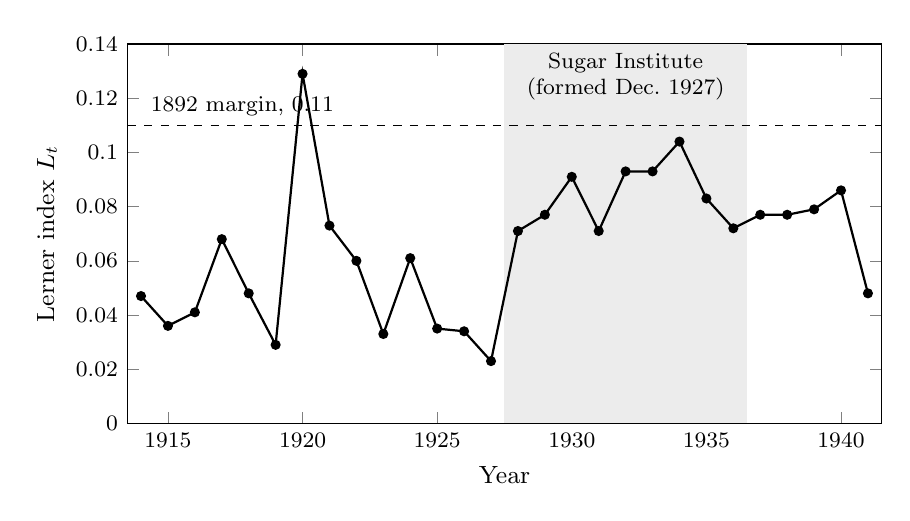
\begin{tikzpicture}
\begin{axis}[
  width=0.92\textwidth, height=6.4cm,
  xmin=1913.5, xmax=1941.5, ymin=0, ymax=0.14,
  xlabel={Year}, ylabel={Lerner index $L_t$},
  xtick={1915,1920,1925,1930,1935,1940},
  x tick label style={/pgf/number format/1000 sep={}},
  ytick={0,0.02,0.04,0.06,0.08,0.10,0.12,0.14},
  y tick label style={/pgf/number format/fixed,/pgf/number format/precision=2},
  tick label style={font=\footnotesize}, label style={font=\small},
  clip=false]
\fill[gray!15] (axis cs:1927.5,0) rectangle (axis cs:1936.5,0.14);
\node[font=\footnotesize, align=center] at (axis cs:1932,0.128) {Sugar Institute\\(formed Dec.\ 1927)};
\draw[dashed] (axis cs:1913.5,0.11) -- (axis cs:1941.5,0.11);
\node[font=\footnotesize, anchor=south west] at (axis cs:1914,0.11) {1892 margin, 0.11};
\addplot[thick, mark=*, mark size=1.4pt] coordinates {
 (1914,0.047) (1915,0.036) (1916,0.041) (1917,0.068) (1918,0.048) (1919,0.029) (1920,0.129)
 (1921,0.073) (1922,0.060) (1923,0.033) (1924,0.061) (1925,0.035) (1926,0.034) (1927,0.023)
 (1928,0.071) (1929,0.077) (1930,0.091) (1931,0.071) (1932,0.093) (1933,0.093) (1934,0.104)
 (1935,0.083) (1936,0.072) (1937,0.077) (1938,0.077) (1939,0.079) (1940,0.086) (1941,0.048)};
\end{axis}
\end{tikzpicture}
\caption{Lerner index of cane sugar refining, 1914--1941, computed from direct marginal cost,
$L_t = \frac{p^{\mathrm{ref}}_t - 1.075\,p^{\mathrm{raw}}_t - 0.60}{p^{\mathrm{ref}}_t}$. The shaded years are
1928--1936. The dashed line is the 1892 margin, which \citet{GenesoveMullin2001} propose as a realistic
monopoly benchmark. Redrawn from \citet{GenesoveMullin2001}, Table~1, column (4).}\label{fig:13-gm-lerner}
\end{figure}

The Lerner index uses list prices, and secret discounts were the reason the Institute was founded. Genesove and
Mullin argue that this bias strengthens their conclusion. The argument takes one line. Let the average
transaction price be $p^{a}_t = p^{\mathrm{ref}}_t - d_t$, where $d_t \ge 0$ is the average secret discount.
Marginal cost is measured directly, so the change in the transaction margin is
\begin{equation}\label{eq:13-gm-lowerbound}
  \Delta\left(p^{a}_t - mc_t\right) = \Delta\left(p^{\mathrm{ref}}_t - mc_t\right) - \Delta d_t
  \;\ge\; \Delta\left(p^{\mathrm{ref}}_t - mc_t\right)
  \quad\text{whenever } \Delta d_t \le 0 .
\end{equation}
If the Institute eliminated secret concessions, or at least did not increase them, the rise in the list margin is
a lower bound on the rise in the transaction margin.

How close did the refiners come to monopoly? The inverse elasticity rule of \cref{sec:02-monopoly} gives a
monopoly Lerner index of $\frac{1}{\varepsilon}$. With the demand elasticity of 1.75 that Genesove and Mullin
estimated for 1890--1914, the monopoly Lerner index is $\frac{1}{1.75} = 0.57$, far above anything in
\cref{tab:13-gm-t1}. The authors give two reasons for the gap. The growth of beet sugar after the First World War
raised the elasticity of demand facing cane refiners, and the refiners wanted to deter foreign and domestic
entry. They propose 11 percent as a realistic benchmark. That was the margin in 1892, when both the margin and
American Sugar Refining's market share (92 percent) reached their peaks. Over 1928--1935 the Lerner index
averaged 0.085 (our computation), about three quarters of that benchmark, as the authors state. The benchmark has
a structural reading. If 0.11 were the Lerner index of a firm pricing optimally against its residual demand, the
inverse elasticity rule would put that residual elasticity at $\frac{1}{0.11} \approx 9$ (our computation). A
perceived elasticity five times the market elasticity is consistent with pricing to limit entry and imports.

Quantities tell the same story more weakly. The output of the Atlantic refiners fell when the Institute began,
though only a little, because sugar demand is inelastic. Output kept falling during the Great Depression, but much
less than the 24 percent fall in total industrial output (p.~382). Rivals outside the agreement expanded. The
share of imported refined sugar, almost all of it Cuban, rose from under half a percent to 6 percent in the
Institute's first year and to almost 15 percent in 1933. The Sugar Act of 1934 then cut it to 11 percent by
legislative fiat. Coca-Cola, the largest buyer of refined sugar, switched entirely to foreign suppliers. The beet
share rose from an average of 15.4 percent in 1924--1927 to 17.7 percent in 1928--1931, but its year-to-year
variability prevents a firm attribution to the Institute.

\casehead{Collusion by rules}
Genesove and Mullin describe the Institute as implicit collusion on price combined with explicit collusion on
business practices (p.~383). Rule number one required ``open prices and publicly announced terms.'' Prices
were posted on the refiners' bulletin boards, the Institute was notified of every change in prices and pricing
methods, and changes were announced by 3:00 p.m. These provisions continued existing practice. The more
important existing practice was the \emph{moves system}. An announced price decrease took effect immediately,
while an increase took effect only after a day. Buyers purchased a month's supply at a time, so they waited after
a decrease until other refiners matched it, which they always did. Reactions often came within minutes. Price
competition therefore preceded trade.

\begin{remark}[Why the moves system leaves only secret deviations]\label{rem:13-moves}
Let $N$ refiners sell a homogeneous good at a common list price $p$ with $c < p \le p^m$, and let industry profit
$\pi(p) = (p - c)D(p)$ be increasing on $[c, p^m]$. Suppose that a public price cut to $p' < p$ is matched by
every rival before any buyer purchases. Buyers then split equally among the refiners, and the cutter earns
$\frac{1}{N}\pi(p')$ in the period. Because $\pi$ is increasing on $[c, p^m]$,
\begin{equation*}
  \frac{1}{N}\,\pi(p') < \frac{1}{N}\,\pi(p) .
\end{equation*}
A public cut lowers the cutter's own profit. Only a concession that rivals cannot see, and hence cannot match,
can raise a refiner's share. This is why the Institute worked to raise the probability of detecting secret
concessions and did not try to shorten reaction times (\citealp{GenesoveMullin2001}, pp.~383--384). The
model of \cref{sec:13-transparency-theory} formalizes this probability.
\end{remark}

Almost every contractual term could hide a price cut, so the rules were wide-ranging and detailed.
\Cref{tab:13-gm-rules} lists the five rules that Genesove and Mullin examine, the concession each one closed, and
the cost it imposed. The Institute also disallowed quantity discounts, allowances for returned sugar bags,
long-term contracts and certain credit arrangements. It required refiners to report all sales of damaged sugar,
drew up a list of permissible consignment points, and forbade downstream firms to combine brokerage and storage.
Enforcing the last rule required private investigation and auditing.

\begin{table}[htbp]
\centering
\caption{Sugar Institute rules, the hidden concessions they closed, and their costs}\label{tab:13-gm-rules}
\small
\begin{tabularx}{\textwidth}{@{}>{\raggedright\arraybackslash}p{2.6cm}>{\raggedright\arraybackslash}X>{\raggedright\arraybackslash}X@{}}
\toprule
Rule & Concession it closed & Cost or side effect\\
\midrule
Water-damaged or frozen sugar & Sound sugar shipped to a favored buyer and invoiced as damaged. Each sale now
required ``full details of amount, location, reason and price'' to be circulated. & Discounts on truly damaged
sugar became public.\\
\addlinespace
Credit terms & Varying the grace period that qualified for the customary 2 percent cash discount. & Grace period
fixed at 7 days rather than 14.\\
\addlinespace
Storage & Brokers who ran warehouses cut storage charges in place of the sugar price. & Storage first banned in
buyers' warehouses, then in broker-affiliated ones as refiners switched.\\
\addlinespace
Delivery time & Letting favored buyers take delivery after the contract date, which saved storage and interest
and was a price cut if the basis price rose. & Delivery dates enforced. Weekly reports of undelivered contracts.
A secondhand market sold overbought sugar at discounts of 5 to 20 cents.\\
\addlinespace
Freight & Rebates on freight rates that the Interstate Commerce Commission did not regulate, especially private
water charters. & Charters registered, uniform rates required, written promises not to rebate. Then delivered
pricing with a refusal to sell f.o.b.\ refinery.\\
\bottomrule
\end{tabularx}

\smallskip
\begin{minipage}{0.95\textwidth}\footnotesize
Notes: Compiled from \citet{GenesoveMullin2001}, Sections II, III and VI (pp.~383--387 and 390--392). The
organization into columns is ours.
\end{minipage}
\end{table}

The rules were costly. A monopolist could have discriminated among customers and exploited efficiencies that the
rules forbade. When large buyers in Buffalo asked to receive sugar by water barge, even at the higher rail rate,
the Institute refused for fear of creating an opportunity for discounts. The move to delivered pricing led
refiners to replace brokers in barge transport. Between 1928 and 1931, barge shipments by refiners rose by 400
percent while those by customers fell by two thirds. Large customers denied quantity discounts threatened to
integrate backward, as the grocery chain A\&P did. The ban on long-term and tolling contracts also sacrificed
efficiencies. Place was even prepared to forgo allocating production by cost. He feared that local differences in
loading costs would lead to different rates, writing that ``those enjoying more economical loading conditions
can pocket the profits.'' The District Court judge put it succinctly (p.~384, fn.~14). The refiners
``preferred to have all sugar sold in any given trade areas at precisely the same prices and terms'' over
economies in distribution.

Genesove and Mullin consider an alternative reading in which the rules suppressed nonprice competition directly.
Contractual harmonization usually chose the lower ``quality.'' The grace period was set at 7 days, and the number
of consignment points was cut by half. They find this reading incomplete for three reasons. It does not explain
many rules, such as the ban on quantity discounts or the notification rules discussed below. The number of sugar
grades was never restricted, although grade proliferation was costly to small refiners. Most persuasively, the
reading misses the stated intermediate goal of eliminating discrimination among customers, the first principle
of the Code of Ethics. They conclude that suppressing nonprice competition complemented harmonization but was
not its purpose.

\casehead{An incomplete agreement and its governance}
The initial agreement was incomplete in the sense of the theory of the firm. No one could foresee and enumerate
all contingencies. The refiners told the court that the Code ``could not be, self-operative'' and required
``interpretation and administration and consultation.'' The weekly meetings completed the contract in three ways.
They answered minor questions the Code left open. May damaged sugar be sold under a price guarantee? No. Do
30-day contracts end on the 30th day or on the same day of the next month? The former. They modified rules that
proved unworkable. The original policy charged the regulated all-rail rate whatever the mode of transport. This
leveraged each refiner's power in its hinterland into contested markets such as the Great Lakes, and cheaper water
routes offered too much arbitrage. A later regime of limited differential rates also failed. The refiners then
moved to delivered prices with a refusal to sell f.o.b.\ refinery. The move was presented as independent action.
The Place memos show that it was coordinated over several meetings in one week of April 1929. It had been delayed
for over a year for fear of the antitrust authorities. Finally, the meetings closed loopholes. Each rule that shut
one channel for secret concessions opened another, less effective one, much as taxpayers respond to a new tax
rule.

The meetings formalized their decisions as Code Interpretations, which took on a quasi-judicial character.
Participants spoke of evidence and precedent. Institute counsel called the Interpretations ``absolutely
indispensable,'' since ``even national laws must be `interpreted' by the Courts.'' Genesove and Mullin argue that
legal principles helped complete the contract. One decision covered many later incidents, disputes were
minimized, and participants could anticipate one another's responses.

A natural worry is that frequent meetings invite renegotiation out of punishments \citep{McCutcheon1997}.
Genesove and Mullin see no sign of it. The refiners chose weekly meetings and no one proposed meeting less often.
Threats were never retracted, and no firm bargained its way out of a punishment (p.~396).

\casehead{Prior notification}
Institute rules required a firm to notify the other members before selling damaged sugar, introducing new private
brands, or changing any terms of trade. Firms also notified one another when no rule required it. Revere, a Boston
refiner, told the Institute before it considered lowering its rail rates to the water rate. Arbuckle announced a
cut in freight rates privately to the members before announcing it publicly. Notification served two purposes.
First, it removed the lag before retaliation in nonprice dimensions, complementing open price announcements. Full
collusion is possible when firms can respond to deviations before consumers act \citep{Bhaskar1989}. In the
language of \cref{sec:13-transparency-theory}, notification makes a nonprice change visible with probability one
before it can steal customers.

Second, notification served the individual interest of the notifying firm. Some actions are profitable once
rivals have responded but steal market share if rivals do not anticipate them. Stealing share risks retaliation.
A Godchaux representative praised Savannah, which explained its need to change its business methods at a Board
meeting before announcing anything. As a result, its ``subsequent announcements, because understood, did not
cause any upheavals.'' Genesove and Mullin describe a two-level agreement. The lower level was a precise set of codes and
resolutions. The higher level was an understanding that a refiner could withdraw from a lower-level rule if it
first told the others. All the cases they record concern an easing of terms of trade. This distinguishes them
from the familiar case of advance notice of price increases, where notice coordinates a move that is profitable
only if all firms follow.

\casehead{Ex post determination of fault}
The meetings were also a forum for accusation and rebuttal. In March 1929, American charged Federal with secretly
cutting prices by loading barges without charge. The dispute turned on what ``f.o.b.'' meant, and Federal
may have believed that other firms loaded barges the same way. As in \citet{GreenPorter1984}, the evidence of
cheating was ambiguous. In their model the confounding factor is a fall in demand. Here it was a
misunderstanding about the terms of the agreement. In other cases it was an
external event, such as a shortage of barges or vacuum pans. An accusation could also be factually wrong. An
Institute investigator once reported a concession on one barrel of caked sugar as a concession on a much larger
amount of powdered sugar.

Genesove and Mullin give two reasons why firms investigated before retaliating. A firm may not have intended to
break the agreement, and the Institute let an accused firm prove its innocence on factual or logical grounds. In
their words, the Institute ``raised the signal-to-noise ratio of indicators of cheating.'' An accuser acting alone
also risked being accused of cheating itself. Evidence that only the accuser could observe was therefore
insufficient, and accusers needed evidence that others could verify. In one case an investigator produced an invoice that seemed to show a sale
from Godchaux to Edgar, a Detroit broker that also ran storage. Place examined the invoice and judged it part of
Godchaux's bookkeeping, and the refiners were notified of ``the error which apparently had been made.''
\Cref{cor:13-false-alarms} below shows why lowering the rate of false accusations relaxes the incentive
constraint.

\casehead{Cheating and retaliation}
In the theory of implicit collusion, every deviation by a player is treated the same way, whatever its nature or
timing. Genesove and Mullin observe something quite different. Firms did cheat. A Detroit chain store received a
secret concession when it switched from National to Spreckels. Spreckels overpaid truckers, who then worked a few
hours ``free'' for certain customers. Arbuckle knowingly sold to a dummy corporation that fronted for Edgar.
Cheating was worst in the South. Godchaux accepted a contract with a price guarantee for delivery by water barge
whose movements it agreed not to trace. Texas City accepted a 42-day contract, and its owner offered to fire his
top three executives over it. Colonial offered a 6-cent rebate to large buyers, and in Tampa postdated checks were
used to give credit (p.~390).

Outside the South, none of these violations led to competitive prices as in \citet{GreenPorter1984}, let alone
to subcompetitive prices as in \citet{AbreuPearceStacchetti1986}. The usual sequence was that fault was
determined, the refiner confessed, justified itself or blamed its broker, and the practice stopped. Longer or open
violations were matched. When one firm openly lowered its rail rate to the barge rate, the others lowered theirs
to the same level. When the Pacific refiners gave a freight allowance, American announced that it would match it.
Matching was in degree and in kind. The response stayed within the instrument of the violation, although
\citet{BernheimWhinston1990} show that punishing across all instruments strengthens collusion. When McCahan
concluded that some refiners were not enforcing contract time limits, Place first threatened, and then with
others carried out, a refusal to enforce McCahan's terms. Matching was even institutionalized. Each refiner
reported its undelivered contracts for each price move, the reports circulated weekly, and an unannounced
understanding let all refiners spread deliveries over as many days as the most delayed refiner.

Massive retaliation came only after large-scale cheating in several dimensions, and only in the South. As early as
June 1929 an investigator reported the Code ``dead in the water'' in Texas. C\&H refused to discuss any single
violation there. It threatened to ask for ``the entire suspension of the Code of Ethics in the Texas territory''
so that all refiners could ``fight fire with fire.'' Elsewhere in the South, Savannah was dissuaded
from resigning by a resolution that allowed members to ``meet the competition of Hershey,'' a Cuban refiner
outside the Institute. The condition was that the competitor and the territory be announced to the Institute
first. The agreement could be suspended, but only with prior notification.

Genesove and Mullin summarize the contrast in terms of statistical errors. In the Green and Porter equilibrium,
firms accept punishing when no one has cheated so that cheating never occurs. The refiners chose the opposite end
of the trade-off. They accepted some cheating so as not to punish inappropriately, and they sustained imperfect
collusion because wholesale cheating did meet massive retaliation. Two features of the industry help explain this
choice. Refiners sold through brokers, who often dealt exclusively with one refiner and earned a fixed commission
on every sale. A broker gained much more from stealing a customer than its refiner did. Brokers' cheating added
noise to demand and let refiners hide behind their brokers. The same agency relation made punishment costly,
since selling agents cannot easily be told to follow one set of rules one day and another the next. Matching also
has a known robustness, as in the ``tit for tat'' strategies of \citet{Axelrod1984}, and it fitted the ethic of
nondiscrimination in the Code.

\casehead{What the refiners did not do}
In the model of \citet{GreenPorter1984} firms monitor a public signal, the market price, and never see their
rivals' outputs (\cref{sec:13-jec-setting}). \citet[p.~90]{GreenPorter1984} note that noisy market-share
information could serve as the signal instead. Genesove and Mullin take this broader reading. They describe
Green-Porter and its offshoots as models in which cheating is inferred from a firm's market share (p.~394). Some
models of imperfect monitoring also transfer share to firms that lost it. Market-share data were available to the
refiners at low frequency, but they rarely used them this way. Genesove and Mullin find only four such incidents in nearly a hundred meetings
over 18 months (p.~394). In one, Arbuckle's low share was blamed on its strict contract enforcement, and the
possibility that American's advertising was responsible was dismissed because others' sales had not fallen. The
reason for a fall in share mattered, unlike in the market-share reading of the theory. There was no mechanism for reallocating market shares.
American twice proposed market-sharing schemes in 1929, but neither came with an enforcement mechanism and
Institute counsel would not allow discussion that ``could bring actual results.'' There were no mergers, and
calls for coordinated market withdrawals went unfulfilled. The contrast with the quota-and-transfer cartels of
\citet{HarringtonSkrzypacz2011}, discussed in \cref{sec:13-imperfect}, is sharp.

\casehead{Interpretation, critiques and contribution}
The Institute did more than host communication. It was a neutral party that could audit members and aggregate
self-reported statistics into confidential industry totals. Firms could also use it as a scapegoat or a
commitment device in bargaining with brokers and buyers. Genesove and Mullin draw three lessons for theory.
Collusive agreements are incomplete and need governance. Communication within the agreement is rich, with prior
notification and ex post determination of fault. Retaliation is much more restrained than theory predicts,
partly because of selling agents' high-powered incentives. They also stress that Stigler's basic insight
survives. The rules were built by firms that knew each would later want to undermine them.

The evidence has limits. The notes come from one participant at a midsize refinery and cover 18 months of a
nine-year cartel. The performance measures use list prices. A list price is never below the transaction price, so the list
margin bounds the level of the transaction margin from above. Only the rise in the transaction margin is bounded
from below, by the rise in the list margin, and \eqref{eq:13-gm-lowerbound} gives that bound only if secret
discounts did not grow. There is no counterfactual for what prices would have been without the
Institute in the Great Depression, and the rise in imports shows that the cartel's market power was limited.
Inferring strategies from what participants said requires trusting that they described their reasoning
accurately, a premise the authors defend. The forgone efficiencies are public, while those in
\citet{AtheyBagwellSanchirico2004} are private information, so that theory cannot explain why the refiners gave
them up. Genesove and Mullin's own explanation is that exploiting the efficiencies would have destroyed the
homogeneity of practices that made pricing transparent. The paper's contribution is to show that cartels can
invest in detection itself, through rules that make contracts comparable and through a forum that judges
evidence. It also poses the puzzle of tolerated cheating that \citet{BernheimMadsen2017} later addressed
(\cref{sec:13-imperfect}).

\subsection{Price wars in pre-1914 sugar refining}\label{sec:13-gm-pricewars}

The same industry provides a test of what price and cost data can say about conduct. \Cref{sec:03-sugar-wars}
analyzes the two post-entry price wars of 1890--1914 studied by \citet{GenesoveMullin1998}. They followed the
entry of Spreckels (January 1890 to February 1892) and of Arbuckle and Doscher (September 1898 to April 1900).
Conduct is $\theta_t = \theta_0 + (\theta_1 - \theta_0)\mathit{WAR}_t$. Direct cost data give
$\theta_0 = 0.129$ and $\theta_1 - \theta_0 = -0.127$ in the published article \citep[Table~10]{GenesoveMullin1998},
so conduct in the wars
was $0.002$, essentially competitive. The NBER working paper on file reports 0.11 and $-0.09$ for the same direct
measures (\citealp{GenesoveMullin1995}, Table~14, column~(9)). Holding marginal cost fixed across regimes, the
nonlinear instrumental-variables estimates detect the fall. With linear demand, $\hat\theta_1 - \hat\theta_0 =
-0.112$ (0.069) when $k$ is estimated and $-0.108$ (0.051) when $k = 1.075$ is imposed (\cref{tab:03-gm-pricewars},
Panel A). These two estimates are the same in both versions (working paper, Table~14, columns~(3) and~(4)).

When the cost intercept may also shift in the wars, the same estimator attributes the wars to falling cost. The
estimated cost drop is 10 to 18 cents per hundred pounds and the fall in conduct only 0.015 to 0.024 across
demand forms (\citealp{GenesoveMullin1995}, Table~15). Neither difference is significant. This is
\cref{prop:13-obs-equiv} in real data. Prices and quantities alone cannot separate a switch in conduct from a
switch in cost. Prior information that costs were stable, available here from the technology, breaks the tie.
The Sugar Institute era of \cref{sec:13-sugar-institute} is the same industry a generation later, when the
refiners tried to avoid such wars by rules rather than by punishment.

\subsection{The bromine cartel, 1885--1914}\label{sec:13-bromine}

\casehead{The question}
Why do cartels fight price wars? In \citet{GreenPorter1984} and \citet{AbreuPearceStacchetti1986} (APS
hereafter), price wars are equilibrium punishments. Firms cannot see one another's actions, so they punish after
unfavorable public signals even though no one cheats (\cref{ch:collusion-theory}). An older view, associated with
\citet{Stigler1964}, sees price wars as breakdowns caused by cheating or entry. \citet{Levenstein1997} uses
internal documents of the bromine industry, including contracts, correspondence and minutes of negotiations, to
ask which view fits. She finds that both do, for different wars. Short, mild wars came from imperfect
information. Long, severe wars were part of bargaining over the division of rents.

\casehead{The industry}
Bromine was first produced commercially in 1845. During the Civil War, army medics discovered the sedative
properties of potassium bromide, which became a popular patent medicine for headaches and nervous disorders. In
Europe bromine was used in aniline dyes, but this use was negligible in the United States until after the First
World War. Before 1892 a dozen small firms near the Ohio River, in southeast Ohio and northwest West Virginia,
produced all U.S.\ bromine by pumping and heating underground brine. They sold liquid bromine to
\emph{manufacturing chemists}, larger urban firms that converted it into potassium bromide powder and distributed
it to pharmacies. The two most important were Powers \& Weightman (P\&W) and Mallinckrodt Chemical Works. The only
other significant producers were German potash mines. They belonged to a bromine cartel allied with the German
potash cartel, which had the active support of the German state.

\casehead{The cartel's organization}
Collusive institutions controlled the market for most of 1885--1914, and their form changed three times
(\cref{fig:13-lev-contracts}). In 1885 the National Bromine Company (NBC) contracted with the Ohio River firms to
buy their entire output for five years at a specified price. The contracts forbade sales to anyone else.
Mallinckrodt and P\&W in turn agreed to buy all of the NBC's bromine, and they announced the price of potassium
bromide in coordination. That price rose from 26.5 cents per pound at the end of 1884 to 34 cents right after the
contracts were signed in March 1885. The NBC expired in March 1891. A new pool was not formed until October 1892.
W.~R. Shields of Columbus, Ohio then contracted with each producer to buy its entire output for five years, and he
sold it to Mallinckrodt and P\&W. These two firms agreed with the German cartel not to export, and the Germans
agreed to buy \$25,000 of bromine a year from them.

Herbert Dow's entry changed the industry. His Midland Chemical Company, incorporated in 1892 and merged with the
Dow Chemical Company in 1900, used an electrolytic process. It produced bromine and bromide salts continuously
and more cheaply, and its minimum efficient scale was at least ten times that of an Ohio River producer. Dow never
joined the pool but sold its entire output to Mallinckrodt and P\&W under a one-year contract in 1894. The
contract limited Midland's output and forbade other sales. Two more one-year contracts followed, then a five-year
contract in 1897. In the spring of 1902 Dow ended its cooperation and signed with two rival chemists, Rosengarten
\& Sons and George Merck \& Company. Shields' contracts expired in October 1902 and were not renewed.

\begin{figure}[htbp]
\centering
\tikzset{lbox/.style={draw, rounded corners=1pt, align=center, inner sep=2pt, font=\scriptsize},
         lcart/.style={lbox, fill=gray!25}}
\begin{subfigure}[b]{0.32\textwidth}\centering
\begin{tikzpicture}[>=Stealth]
\node[lbox] (ohio) at (0,3.1) {Ohio River producers\\(about 12)};
\node[lcart] (nbc) at (0,2.0) {National Bromine\\Company};
\node[lcart] (mal) at (-0.95,0.9) {Mallinckrodt};
\node[lcart] (pw) at (0.95,0.9) {P\&W};
\node[lbox] (ph) at (0,-0.15) {Retail pharmacists};
\draw[->] (ohio) -- (nbc);
\draw[->] (nbc) -- (mal); \draw[->] (nbc) -- (pw);
\draw[->] (mal) -- (ph); \draw[->] (pw) -- (ph);
\end{tikzpicture}
\caption{NBC pool, 1885--1891}
\end{subfigure}\hfill
\begin{subfigure}[b]{0.32\textwidth}\centering
\begin{tikzpicture}[>=Stealth]
\node[lbox] (ohio) at (-0.9,3.1) {Ohio River\\producers};
\node[lbox] (dow) at (1.05,3.1) {Midland/\\Dow};
\node[lcart] (sh) at (-0.9,2.0) {Shields};
\node[lcart] (mal) at (-0.95,0.9) {Mallinckrodt};
\node[lcart] (pw) at (0.95,0.9) {P\&W};
\node[lbox] (ph) at (0,-0.15) {Retail pharmacists};
\draw[->] (ohio) -- (sh);
\draw[->] (sh) -- (mal); \draw[->] (sh) -- (pw);
\draw[->] (dow) -- (mal); \draw[->] (dow) -- (pw);
\draw[->] (mal) -- (ph); \draw[->] (pw) -- (ph);
\end{tikzpicture}
\caption{Shields pool, 1892--1902}
\end{subfigure}\hfill
\begin{subfigure}[b]{0.32\textwidth}\centering
\begin{tikzpicture}[>=Stealth]
\node[lbox] (ohio) at (-0.45,3.1) {Ohio River\\producers};
\node[lcart] (dow) at (-0.45,2.0) {Dow Chemical};
\node[lbox] (oth) at (1.45,2.0) {Other\\non-retail\\customers};
\node[lcart] (mal) at (-1.35,0.9) {Mallinckrodt};
\node[lcart] (pw) at (0.0,0.9) {P\&W};
\node[lcart] (me) at (1.2,0.9) {Merck};
\node[lbox] (ph) at (0,-0.15) {Retail pharmacists};
\draw[->] (ohio) -- (dow);
\draw[->] (dow) -- (oth);
\draw[->] (dow) -- (mal); \draw[->] (dow) -- (pw); \draw[->] (dow) -- (me);
\draw[->] (mal) -- (ph); \draw[->] (pw) -- (ph); \draw[->] (me) -- (ph);
\end{tikzpicture}
\caption{After 1910}
\end{subfigure}
\caption{Contractual relationships in the bromine industry. Arrows show the flow of bromine under the
contracts. Shaded boxes reproduce the filled boxes of the original figures, which mark the firms at the center of
each arrangement. In panel (c), P\&W is Powers-Weightman-Rosengarten, as Dow's 1908 contracts name it. Redrawn from
\citet{Levenstein1997}, Figures~2--4.}\label{fig:13-lev-contracts}
\end{figure}

International relations followed a similar path. In September 1902 Dow and the German bromine combine agreed in
writing that neither would export potassium bromide to the other's home market. Dow confirmed the agreement and
soon began exporting to Europe in secret. In 1905 the Germans abrogated their side and entered the U.S.\ market.
A detailed agreement at the end of 1908 ended the resulting war. Dow and the Germans set prices jointly in the
United States, Europe and the rest of the world. Dow withdrew from Europe for a payment of \$32,000 a year and
received a one-third share of sales in the rest of the world, and the Germans withdrew from North America. Dow
also signed ten-year contracts to supply all the bromine needs of three manufacturing chemists. It kept the price
of potassium bromide below 20 cents for a year and a half, a price at which the Ohio River firms could not sell
profitably. In May 1910 it contracted to buy the entire output of all but one of them on a sliding scale tied to
the published price. Prices then rose slowly but steadily until the First World War.

\casehead{Evidence of success}
The firms' account books have not survived, so Levenstein assembles indirect evidence. Midland paid its first
dividend after its 1894 contract, followed by regular monthly dividends of two to five percent, when annual
interest rates in the region averaged less than 6.5 percent. Dow, Shields, Mallinckrodt and the Germans made
trans-Atlantic trips for no purpose other than negotiating collusive agreements. Shields supported his family for
a decade on the rents he kept for organizing the pool.

Prices give stronger evidence. The price of bromine fell from six dollars a pound before the Civil War to 30
cents in 1875. It fell another 7 percent by 1880 and almost 30 percent more by 1884. The NBC reversed the trend. The average price of potassium bromide during the NBC pool, 34.08 cents, was almost 10 percent above
the 31.07 cents of the preceding five years. When the NBC contracts ended in 1891, prices fell by almost 30
percent. The Shields pool averaged 40.88 cents, 65 percent above the 24.75 cents between the two pools (the paper
says 60 percent) and 31.6
percent above the prices of 1880--1885. When the Shields contracts expired in 1902, the price fell 43.2 percent
in one month. Between 1902 and 1914, the average price was 29.3 cents during cooperation and 16.8 cents
otherwise, almost 75 percent higher. The price jumped from 13 to 19 cents on December 21, 1908, the day the Dow
and German agreement took effect. The same comparisons hold for prices deflated by a wholesale chemical price
index. For example, real prices after 1902 were 74 percent higher during cooperation (WP pp.~9--11, fns.~19--23).

Costs confirm that prices exceeded marginal cost. Dow estimated the marginal cost of a pound of bromine under the
Ohio River process at 12 cents. Shields paid the Ohio River producers 16 cents in the first year of his contracts,
rising by 2 cents a year to 22 cents. For potassium bromide, Levenstein estimates the cost of manufacture as
\begin{equation}\label{eq:13-lev-cost}
  TC(Q) = Q\left(0.85\,P_{\mathrm{Br}} + 0.6\,P_{\mathrm{KOH}} + C_{\mathrm{mc}}\right).
\end{equation}
Here $P_{\mathrm{Br}}$ is the contract price of bromine and $P_{\mathrm{KOH}}$ the market price of potash. The
term $C_{\mathrm{mc}} = 4$ cents is the chemists' processing and distribution cost per pound. During the Shields pool the
price averaged 40.9 cents and this cost 24.1 cents, a markup of almost 70 percent (WP Figure~5). The correlation
between changes in price and changes in cost was $-0.042$. Dow's own cost of potassium bromide was about 8 cents
before 1902, while its 1897--1902 contract paid 25 cents. Prices were also more stable under cooperation.
They changed on average every 41.1 weeks during cooperation and every 11.5 weeks otherwise. Within the pool years
the figures were 35 and 6.8 weeks, and after 1902 they were 64.7 and 17.5 weeks. Many firms announcing prices
independently raise the chance that some price changes in a given week.

\casehead{How close to monopoly}
Levenstein compares the pool price with the prices that monopoly, Cournot and perfect competition would produce.
She considers three linear inverse demand curves for potassium bromide. Each is consistent with aggregate data
and is fitted through the average prices and outputs of two years:
\begin{equation}\label{eq:13-lev-demand}
  \text{I: } P = 78 - 0.077\,Q, \qquad
  \text{II: } P = 67 - 0.038\,Q, \qquad
  \text{III: } P = 173 - 0.203\,Q .
\end{equation}
Prices $P$ are in cents per pound and quantities $Q$ in thousands of pounds a year. Demand I uses 1895 and 1909, II uses 1896 and
1908, and III uses 1897 and 1909. Each firm's cost is \eqref{eq:13-lev-cost} plus a fixed cost, evaluated at
$P_{\mathrm{Br}} = 12$ (Dow's marginal cost estimate) and $P_{\mathrm{KOH}} = 4$ (the average potash price in the
pool period). Marginal cost is therefore constant at
\begin{equation}\label{eq:13-lev-mc}
  c = 0.85 \times 12 + 0.6 \times 4 + 4 = 10.2 + 2.4 + 4 = 16.6 \text{ cents.}
\end{equation}

\begin{example}[Reproducing Levenstein's Table~2]\label{ex:13-lev-cournot}
Let inverse demand be $P = a - bQ$ and let $N$ firms have constant marginal cost $c$. Firm $i$ maximizes
$(a - bQ - c)q_i$. Its first-order condition is
\begin{equation*}
  a - bQ - c - b\,q_i = 0 .
\end{equation*}
In a symmetric equilibrium $q_i = \frac{Q}{N}$. Substituting,
\begin{equation*}
  a - c = bQ\left(1 + \frac{1}{N}\right)
  \quad\Longrightarrow\quad
  Q = \frac{N}{N+1}\,\frac{a - c}{b}, \qquad
  P = a - bQ = \frac{a + Nc}{N+1}.
\end{equation*}
For Demand I, $\frac{a - c}{b} = \frac{78 - 16.6}{0.077} = 797.4$ thousand pounds, the competitive output.
Monopoly ($N = 1$) gives $Q = 398.7$ and $P = \frac{78 + 16.6}{2} = 47.3$ cents. Duopoly gives $Q = 531.6$ and
$P = \frac{78 + 33.2}{3} = 37.1$. Twelve firms, about the number active in 1891, give $Q = 736.1$ and
$P = \frac{78 + 199.2}{13} = 21.3$. Competition gives $P = c = 16.6$. These are exactly the entries of
\cref{tab:13-lev-t2}.
\end{example}

\begin{table}[htbp]
\centering
\caption{Monopoly, Cournot and competitive outcomes for potassium bromide}\label{tab:13-lev-t2}
\small
\begin{tabular}{@{}lccccc@{}}
\toprule
 & \multicolumn{3}{c}{Demand I} & Demand II & Demand III\\
\cmidrule(lr){2-4}\cmidrule(lr){5-5}\cmidrule(l){6-6}
Number of firms & $q_i$ & $Q$ & $P$ & $P$ & $P$\\
\midrule
1 (joint maximum) & 398.7 & 398.7 & 47.3 & 41.8 & 94.8\\
2 & 265.8 & 531.6 & 37.1 & 33.4 & 68.7\\
12 & 61.3 & 736.1 & 21.3 & 20.5 & 23.6\\
$\infty$ & & 797.4 & 16.6 & 16.6 & 16.6\\
\midrule
\multicolumn{6}{@{}l}{Pool average price, 1885--1902, excluding price wars: 38.6 cents}\\
\bottomrule
\end{tabular}

\smallskip
\begin{minipage}{0.92\textwidth}\footnotesize
Notes: Reproduced from \citet{Levenstein1997}, NBER working-paper version, Table~2. Quantities in
thousands of pounds a year, prices in cents per pound. Demand functions in \eqref{eq:13-lev-demand}, marginal
cost 16.6 cents from \eqref{eq:13-lev-mc}. The Demand III entry for 12 firms is printed as 23.6. The printed
quantity of 711.2 and the formula of \cref{ex:13-lev-cournot} both give $P = \frac{173 + 199.2}{13} = 28.6$
(our computation), so 23.6 appears to be a misprint.
\end{minipage}
\end{table}

The pool average of 38.6 cents lies between the twelve-firm Cournot price of 21.3 and the monopoly price of 47.3
under Demand I. Levenstein concludes that the pool raised prices above competitive and usually above Cournot
levels, without reaching monopoly. Collusive prices ranged from 19 to 46 cents. The conduct parameter of
\cref{sec:02-conduct} summarizes the pool price in one number. With linear demand the supply relation is
$P = c + \theta bQ$, so $bQ = \frac{a - c}{1 + \theta}$ and $P = \frac{\theta a + c}{1 + \theta}$. Solving for
$\theta$ at the pool price gives
\begin{equation*}
  \theta = \frac{P - c}{a - P} = \frac{38.6 - 16.6}{78 - 38.6} = \frac{22.0}{39.4} = 0.56
\end{equation*}
(our computation). This lies between symmetric Cournot duopoly ($\theta = \frac{1}{2}$) and joint profit
maximization ($\theta = 1$).

Levenstein also measures the welfare cost of the pool. At 38.6 cents, Demand I gives an output of
$\frac{78 - 38.6}{0.077} = 511.7$ thousand pounds and revenue of \$197,500 (our computation), matching the
\$197,516 she reports. She reports a deadweight loss of \$44,568 a year, less than six
hundredths of a cent per person in 1900. The loss is about 23 percent of industry revenue (our computation), although
the paper says about 25 percent. The triangle between Demand I and the marginal cost of
\eqref{eq:13-lev-mc} is smaller. It equals $\frac{1}{2}(38.6 - 16.6)(797.4 - 511.7) = 3{,}143$ thousand
cent-pounds, or about \$31,400 (our computation).\footnote{Her figure is matched by a marginal cost of about 12.4
cents (our computation). The paper does not state which cost benchmark the deadweight loss uses.}

\casehead{Testing the order of the regime process}
Green and Porter's trigger strategies imply wars of fixed length $T-1$, so the regime process is Markov of order
$T-1$. In APS the length of a war is random and the regime follows a first-order Markov process. Levenstein applies
the test of \citet{BerryBriggs1988}, described in \cref{sec:13-tests}, to two regime series for 1885--1914, one
weekly and one monthly. Each series sets $I_t = 1$ when the firms collude and $I_t = 0$ otherwise. The series
come from reports of collusive activity in the \textit{Oil, Paint and Drug Reporter} and from Dow's papers, and
prices were not used to build them. She did not estimate regimes by switching regressions, as \citet{Porter1983}
did. Demand shifted with regime changes because buyers speculated on whether a break in prices would last, so
the supply relation was not stable across regimes (WP p.~16, fn.~35).

The statistic is $W$ of \eqref{eq:13-bb-test}, which compares the conditional frequencies $\hat p_h$ across
histories $h$ that share the same last period. With a single restriction it reduces to a squared $t$-statistic for
the difference of two frequencies. In the monthly two-period test, the histories $(I_{t-2}, I_{t-1}) = (0,0)$ and
$(1,0)$ have $\hat p = 0.068$ with $N = 73$ and $\hat p = 0.167$ with $N = 6$. (Levenstein's tables list histories
in the order $(t-1, t-2)$.) The statistic for their equality is
\begin{equation*}
  W = \frac{(0.068 - 0.167)^2}{\frac{0.068 \times 0.932}{73} + \frac{0.167 \times 0.833}{6}}
    = \frac{0.00980}{0.00087 + 0.02318} = 0.408 ,
\end{equation*}
which reproduces her Table~3 (our computation). Levenstein treats a restriction as untestable when one of its cells
has $\hat p_h \in \{0, 1\}$, and hence zero estimated variance (WP p.~17). She drops such restrictions. In the
monthly series this leaves one restriction, hence one degree of freedom. In the weekly series every restriction
involves a degenerate cell, so she reports no statistic. For those cells she computes instead the probability, under
the first-order null, of the run that occurred. For example, six continued weeks of collusion after a collusive
week have probability $0.994^{6} = 0.965$ when the continuation probability is 0.994. No such probability falls
below 0.68.

\begin{table}[htbp]
\centering
\caption{The regime process of the bromine cartel}\label{tab:13-lev-markov}
\small
\begin{tabular}{@{}lcc@{}}
\toprule
 & Weekly series & Monthly series\\
\midrule
\multicolumn{3}{@{}l}{\textit{Panel A. Transition probabilities (Table 5)}}\\
$\Pr(I_t = 1 \mid I_{t-1} = 1)$ & 0.995 & 0.978\\
\quad periods with $I_{t-1} = 1$ & 1{,}195 & 275\\
$\Pr(I_t = 1 \mid I_{t-1} = 0)$ & 0.017 & 0.076\\
\quad periods with $I_{t-1} = 0$ & 394 & 79\\
$W$ for history independence, 1 df & 18{,}139.1 & 844.0\\
Implied mean collusive spell (our computation) & 200 weeks & 45.5 months\\
Implied mean price war (our computation) & 58.8 weeks & 13.2 months\\
\addlinespace
\multicolumn{3}{@{}l}{\textit{Panel B. First order against higher order (Tables 3 and 4)}}\\
Two-period alternative, $W$ (p-value) & not computable & 0.408 (0.52)\\
Three-period alternative, $W$ (p-value) & not computable & 0.358 (0.55)\\
\addlinespace
\multicolumn{3}{@{}l}{\textit{Panel C. Kolmogorov-Smirnov test of war durations (Table 6)}}\\
Statistic $d_6$ & 0.352 & 0.340\\
Rejection threshold at the 20 percent level & 0.41 & 0.41\\
\bottomrule
\end{tabular}

\smallskip
\begin{minipage}{0.88\textwidth}\footnotesize
Notes: From \citet{Levenstein1997}, NBER working-paper version, Tables~3--6. Levenstein drops every restriction
that involves a cell with zero estimated variance. In the weekly series every restriction does, so the weekly two-
and three-period tests are not computable. Levenstein reports
``significance'' levels of 0.477 and 0.450, which are one minus the p-values shown. Mean spells use
\cref{lem:13-durations}, for example $\frac{1}{1 - 0.995} = 200$ and $\frac{1}{0.017} = 58.8$.
\end{minipage}
\end{table}

\Cref{tab:13-lev-markov} collects the results. First order cannot be rejected against two- or three-period
alternatives, with p-values of 0.52 and 0.55. History independence is rejected overwhelmingly against a
one-period alternative. A second test compares the distribution of war durations with the geometric distribution
implied by a first-order process. With the weekly exit probability 0.017, the probability that a war has ended
within $t$ weeks is $F(t) = 1 - (1 - 0.017)^t$. The six wars lasted 6, 12, 21, 22, 82 and 201 weeks. The
Kolmogorov-Smirnov statistic is the largest gap between this $F$ and the empirical distribution. It occurs at
$t = 22$, where four of six wars have ended,
\begin{equation*}
  d_6 = \frac{4}{6} - \left[1 - (0.983)^{22}\right] = 0.667 - 0.314 = 0.352
\end{equation*}
(our computation reproduces her statistic). This is below the 20 percent threshold of 0.41, so the first-order
model is not rejected. The mean of the six durations, 57.3 weeks, is close to the predicted 58.8 weeks.

These tests have little power. Six wars cannot distinguish a geometric distribution from many alternatives, and
the mean duration is driven by one war of 201 weeks. A geometric distribution with mean 58.8 weeks has a median
of about 40 weeks, against an observed median of 21.5 weeks (our computation). Levenstein's conclusion from the
statistics is modest. Like \citet{BerryBriggs1988} for the Joint Executive Committee, she finds the bromine
regimes closer to APS than to Green and Porter. The historical record then raises serious doubts about both.

\casehead{The six price wars}
The trade press announced six price wars, three before Dow's entry and three after it. \Cref{tab:13-lev-t7}
reproduces Levenstein's comparison. An optimal APS punishment is the same after any history, prescribes the same
behavior in every punishment period, and is the worst equilibrium punishment. None of these holds. The initial
drop ranged from 0 to 15 cents, or 0 to 50 percent (1 to 15 cents in the five wars with an initial drop). Prices stayed flat in the first two wars but spiralled down
for 73 and 149 weeks in Pool III and Dow III. The lowest prices ranged from 32.5 to 13 cents. Only Pool III and
Dow III reached the one-shot Cournot level of \cref{tab:13-lev-t2}, and no war pushed price below marginal
cost.\footnote{In Dow III the price fell to 13 cents, below the twelve-firm Cournot prices of
\cref{tab:13-lev-t2}. By 1905 Dow produced more than half of U.S.\ output at a marginal cost below 10 cents, so
the table's Ohio River costs no longer applied (WP fns.~38--39).}

\begin{table}[htbp]
\centering
\caption{Characteristics of the bromine price wars}\label{tab:13-lev-t7}
\small
\setlength{\tabcolsep}{4pt}
\begin{tabularx}{\textwidth}{@{}>{\raggedright\arraybackslash}p{2.2cm}*{6}{>{\centering\arraybackslash}X}@{}}
\toprule
 & Pool I & Pool II & Pool III & Dow I & Dow II & Dow III\\
 & 1886--1887 & 1888 & 1891--1892 & 1902 & 1903 & 1905--1908\\
\midrule
Initial drop (cents) & 2 & 1.5 & 1 & 4 & 0 & 15\\
Initial drop (\%) & 6.0 & 4.4 & 3.0 & 9.1 & 0 & 50\\
Total drop (cents) & 2 & 1.5 & 13 & 19 & 0 & 17\\
Total drop (\%) & 6.0 & 4.4 & 39.4 & 43.2 & 0 & 56.7\\
Duration (weeks) & 22 & 12 & 82 & 6 & 21 & 201\\
Weeks to trough & 1 & 1 & 73 & 6 & 0 & 149\\
Low price (cents) & 32 & 32.5 & 20 & 25 & 25 & 13\\
\addlinespace
Initial cause & Germans cut price to force U.S.\ firms out of Europe & Germans believe U.S.\ firms export to
Europe & NBC expires, dispute over new pool terms & Dow signs with non-pool distributors & Dow tries to raise
price, pool distributors refuse & Germans respond to Dow's entry into Europe\\
\addlinespace
Central cause & Coordination & Information & Coordination & Both & Unclear & Both\\
\bottomrule
\end{tabularx}

\smallskip
\begin{minipage}{0.95\textwidth}\footnotesize
Notes: Reproduced from \citet{Levenstein1997}, NBER working-paper version, Table~7. All prices are
for potassium bromide from the \textit{Oil, Paint and Drug Reporter}. Price-war periods were determined from
reports in that journal and internal documents, independently of prices. ``Unclear'' renders the table's
question mark.
\end{minipage}
\end{table}

\casehead{Two kinds of price war}
Levenstein attributes the differences to different causes. Pool War~II and Dow War~I came from imperfect
information. In 1888 the Germans saw bromides imported into their markets and took them as a sign that
Mallinckrodt and P\&W had exported in violation of their agreement. It is not clear whether the Germans were
mistaken or whether customers outside the agreement resold bromine. In 1902 Mallinckrodt and P\&W read Dow's
contracts with Rosengarten and Merck as a sign that Dow would undercut the pool. They cut their price as soon as the
Shields contracts expired. Both wars were short and ended after an exchange of letters reaffirming the commitment
not to compete on price. After Dow War~I the firms adopted a new device, pricing at the price announced in the
\textit{Oil, Paint and Drug Reporter}, to prevent further misunderstandings. Neither war took prices to Cournot
levels.

Levenstein explains why these wars were mild. More severe punishments would not have been renegotiation-proof.
Members discounted threats to price below marginal cost. Dow's executives assessed the credibility of each threat
and demanded verification of the inventories that Mallinckrodt and P\&W claimed to hold. Threats nonetheless
mattered. In December 1892 Shields wrote to Dow that his contracts gave him the right to annul them ``should a new
producer of bromine appear.'' Midland then agreed to restrict its output and sell only to Mallinckrodt and P\&W.
Between 1894 and 1896 Midland's quota rose from 150,000 to 200,000 pounds a year, while its capacity exceeded
350,000 pounds. Midland accepted a five-year contract limiting it to 200,000 pounds in 1897. It accepted
largely because it believed the chemists held 800,000 pounds of bromine, which they threatened to sell if Midland
did not cooperate.

Pool War~III and Dow War~III were different. They were prolonged by information problems, such as the Germans'
ignorance of Dow's costs, but did not result from them. Firms publicly announced that they would sell below the
old collusive price, and everyone understood the announcements as moves in a renegotiation of the division of
rents. In Dow War~III the Germans offered bromides in New York at 15 cents, half the market price. Dow withdrew
from the U.S.\ market and sold its entire output abroad, a response the Germans had not anticipated. The war
lasted until prices reached all-time lows and Dow's representatives had made three trans-Atlantic trips. Dow
learned the German ``Queensbury rules'' of commercial warfare during the negotiations. One rule gave ``the firm that
shows their ability to get the market in a fight'' the same share in the next truce (WP p.~24). With shares in the next truce tied to shares during the war, prices spiralled down. In
these wars the price war itself shaped the next collusive equilibrium. It was not a punishment that restored the
old one.

\casehead{Learning to avoid price wars}
The 1908 agreement between Dow and the Germans included price-war punishments, but they were never used. When
cheating was suspected, the parties identified the most likely culprit, sometimes by chemical analysis of the
bromide. The culprit then made a cash side payment based on a low estimate of its gain. Such firm-specific
transfers sustain more profitable equilibria than common price wars when outcomes reveal who deviated
\citep{AbreuPearceStacchetti1990,FudenbergLevineMaskin1994}. Levenstein offers two reasons for the change. The
firms learned, having started from the price-war punishments common in other pools of the period. The number of
parties also fell and their identities stabilized, which made it easier to identify a cheater and more worthwhile
to invest in information. Genesove and Mullin cite the tit-for-tat clause in the Dow and German agreement as a
parallel to the Sugar Institute's matching. The transfers anticipate those of \citet{HarringtonSkrzypacz2011}.

\begin{figure}[htbp]
\centering
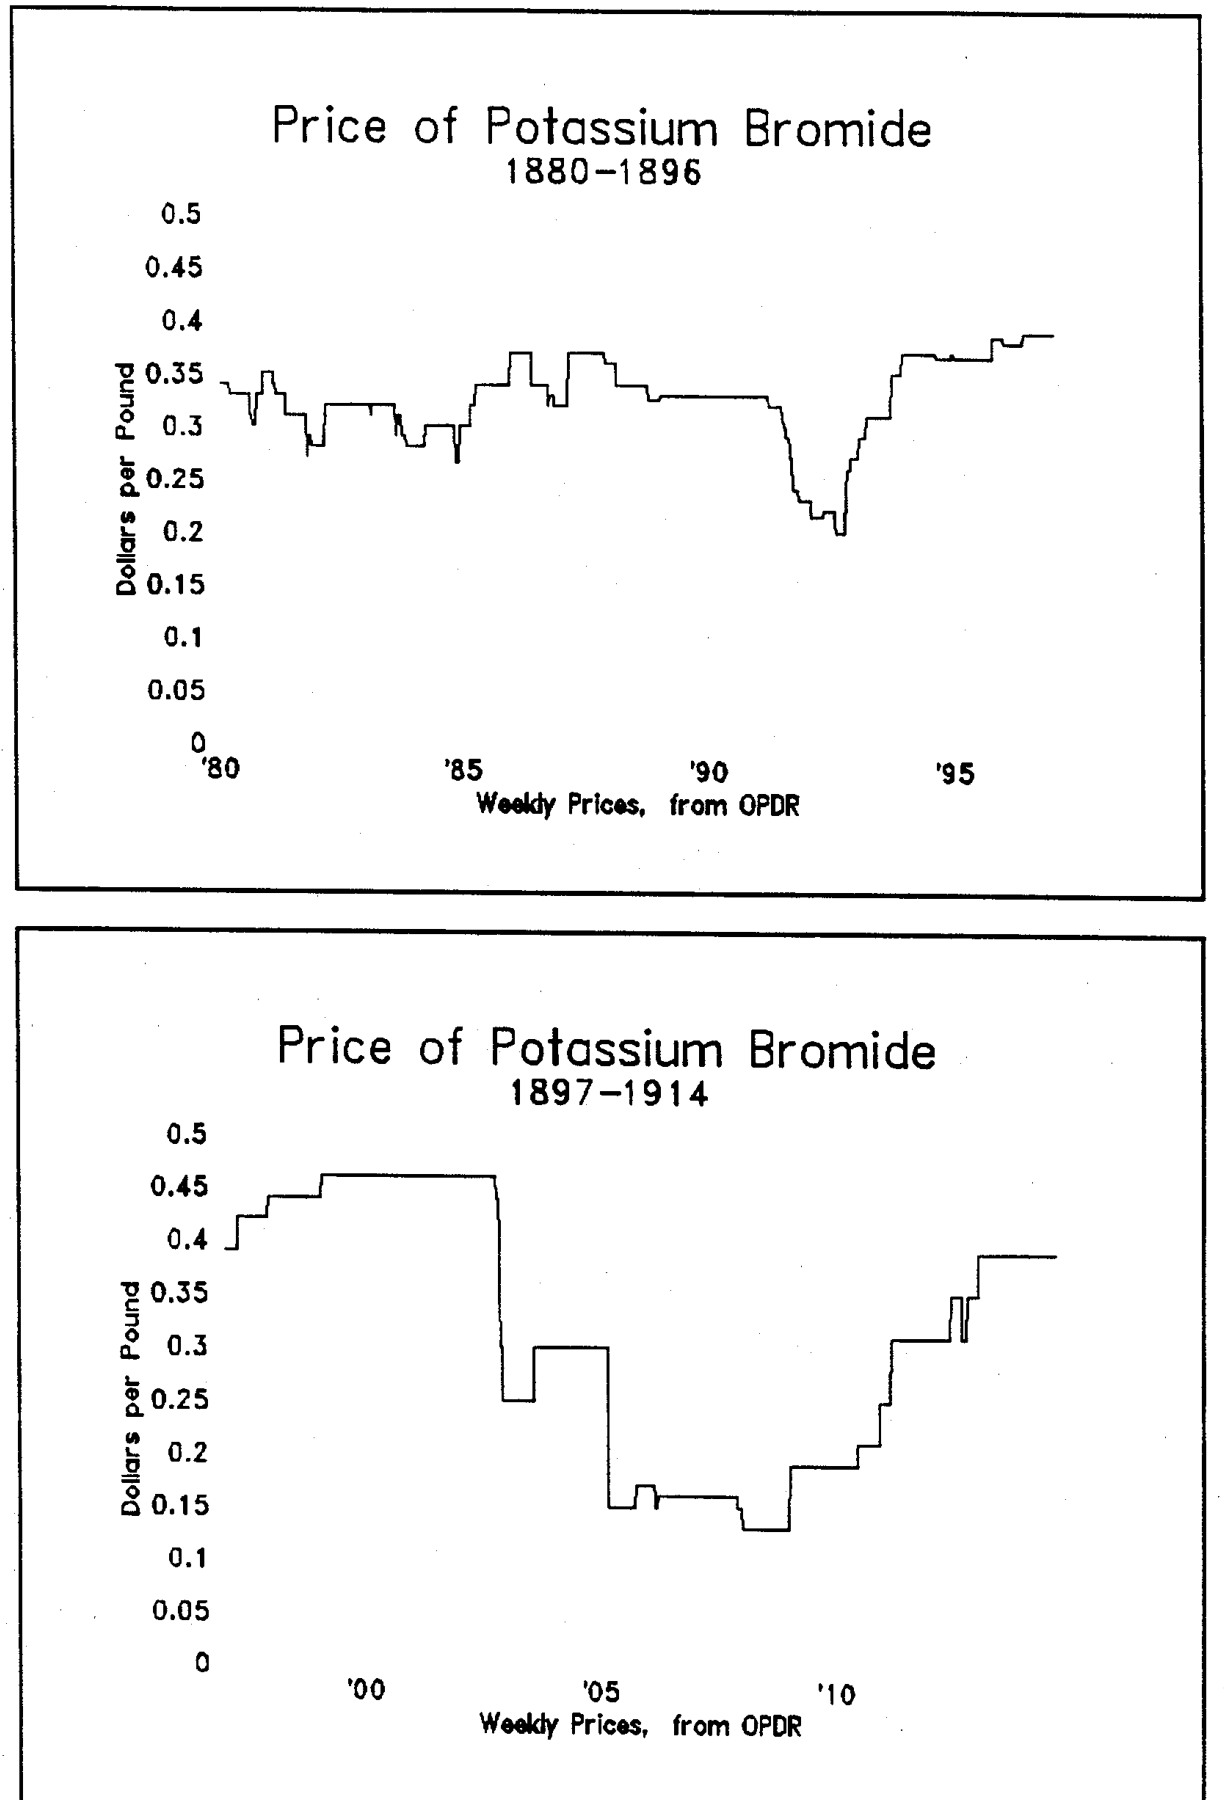
\includegraphics[width=0.62\textwidth]{figures/ch13/levenstein1997_fig1.png}
\caption{Weekly price of potassium bromide in dollars per pound, 1880--1896 (top) and 1897--1914 (bottom), from
the \textit{Oil, Paint and Drug Reporter}. The drop of 1891--1892 is Pool War~III, the collapse of 1902 is Dow
War~I, and the long trough of 1905--1908 is Dow War~III. Source: \citet{Levenstein1997}, Figure~1 (NBER
working-paper version).}\label{fig:13-lev-price}
\end{figure}

\casehead{Assessment}
\Cref{fig:13-lev-price} shows the episodes. The study's strength is its sources. The regime series and the
causes of each war come from documents written by the participants, independently of prices. Its quantitative
parts are weaker. Each demand curve is fitted through two years of aggregate data. Costs come from Dow's estimates
of Ohio River costs, and the deadweight-loss figure cannot be reproduced from the stated cost. The statistical
tests rest on six wars. The paper's contribution is conceptual. Some price wars fit equilibrium punishment under
imperfect monitoring, but they were mild because severe punishments are not credible. Other price wars were
bargaining over the terms of the next agreement, and their severity reflected the stakes of that bargaining.

\section{Information, Transparency and Coordination}\label{sec:13-information}

The Sugar Institute shows firms investing in the detection of secret price cuts. This section asks the same
question from the policy side. What happens when an outside body makes prices more transparent, or when firms use
an information system to signal intentions? We first derive the basic theoretical result, which formalizes
\citet{Stigler1964}. We then study three cases. Danish authorities published firm-specific concrete prices and
prices rose \citep{AlbaekMollgaardOvergaard1997}. The U.S.\ Department of Justice restricted how airlines could
communicate through their fare-publishing system, with temporary effects \citep{Miller2010}. Universities agreed
on financial aid formulas, and their average prices did not change \citep{CarltonBambergerEpstein1995}.

\subsection{Transparency and the incentive constraint}\label{sec:13-transparency-theory}

We embed imperfect detection in the Bertrand supergame of \cref{ch:collusion-theory}. The detection probability
is a reduced-form summary of everything that lets firms infer secret price cuts, such as their own sales, the
trade press, published prices or audits.

\begin{assumption}[Bertrand supergame with imperfect detection]\label{asm:13-transparency}
\leavevmode
\begin{enumerate}[label=(\roman*)]
\item There are $N \ge 2$ firms selling a homogeneous good at constant marginal cost $c$. Industry profit
$\pi(p) = (p - c)D(p)$ is maximized at $p^m$, and $\pi^m = \pi(p^m) > 0$.
\item In each period $t = 1, 2, \dots$ firms set prices simultaneously. The lowest price serves the whole market,
and tied firms split it equally. Firms maximize discounted profit with discount factor $\delta \in (0,1)$.
\item Prices are not publicly observed. At the end of each period a public signal $z_t \in \{0, 1\}$ is realized.
If some firm priced below $p^m$, then $z_t = 1$ with probability $\mu \in (0,1]$. If all firms priced at
$p^m$, then $z_t = 1$ with probability $\mu_0 \in [0, \mu)$.
\item A firm's information about rivals' prices is summarized by the history of public signals.
\end{enumerate}
\end{assumption}

We call $\mu$ the \emph{detection probability} and $\mu_0$ the \emph{false-alarm probability}. Consider the
\emph{public grim-trigger strategy}: charge $p^m$ in period $t$ if $z_s = 0$ for all $s < t$, and charge $c$
otherwise. Pricing at $c$ forever is a Nash equilibrium of every subgame that follows a signal, because each
period's static Bertrand game has the equilibrium $p = c$ with zero profit.

\begin{proposition}[Transparency facilitates collusion]\label{prop:13-transparency}
Under \cref{asm:13-transparency} with $\mu_0 = 0$, the public grim-trigger strategy is a subgame perfect
equilibrium if and only if
\begin{equation}\label{eq:13-transparency}
  \delta \;\ge\; \underline\delta(\mu) = \frac{N - 1}{N - 1 + \mu} .
\end{equation}
The threshold $\underline\delta(\mu)$ is strictly decreasing in $\mu$ and strictly increasing in $N$. It equals
$1 - \frac{1}{N}$ when $\mu = 1$ and tends to 1 as $\mu \to 0$.
\end{proposition}

\begin{proof}
After a signal, the strategies prescribe static Nash play forever, which is subgame perfect. On the collusive
path we use the one-shot deviation principle (\cref{ch:collusion-theory}). On the path each firm earns
$\frac{\pi^m}{N}$ per period, so the value of collusion is
\begin{equation*}
  V = \frac{\pi^m}{N(1-\delta)} .
\end{equation*}
A one-shot deviation to a price above $p^m$ earns zero today and does not change the signal, so it is not
profitable. A deviation to $p < p^m$ captures the market and earns $\pi(p)$, whose supremum over $p < p^m$ is
$\pi^m$. Tomorrow the signal reveals the deviation with probability $\mu$, after which the deviator earns zero
forever. With probability $1 - \mu$ the deviation goes unnoticed and collusion continues with value $V$. Since the
supremum of deviation payoffs is approached but not attained, no deviation is profitable if and only if
\begin{equation*}
  V \;\ge\; \pi^m + \delta(1 - \mu)\,V .
\end{equation*}
Substitute $V$:
\begin{equation*}
  \frac{\pi^m}{N(1-\delta)} \;\ge\; \pi^m + \delta(1-\mu)\,\frac{\pi^m}{N(1-\delta)} .
\end{equation*}
Multiply both sides by $\frac{N(1-\delta)}{\pi^m} > 0$:
\begin{equation*}
  1 \;\ge\; N(1-\delta) + \delta(1-\mu) .
\end{equation*}
Rearrange:
\begin{equation*}
  1 - \delta + \delta\mu \;\ge\; N - N\delta
  \quad\Longleftrightarrow\quad
  \delta\,(N - 1 + \mu) \;\ge\; N - 1 .
\end{equation*}
Since $N - 1 + \mu > 0$, this is \eqref{eq:13-transparency}. Differentiating,
$\frac{\partial\underline\delta}{\partial\mu} = -\frac{N-1}{(N-1+\mu)^2} < 0$ and
$\frac{\partial\underline\delta}{\partial N} = \frac{\mu}{(N-1+\mu)^2} > 0$. The limits follow by substitution.
\end{proof}

\Cref{fig:13-transparency} plots the threshold. Detection matters most when it is poor. With $N = 2$, raising
$\mu$ from 0.2 to 0.4 lowers the threshold from 0.83 to 0.71, while raising it from 0.8 to 1 lowers it only from
0.56 to 0.50.

\begin{figure}[htbp]
\centering
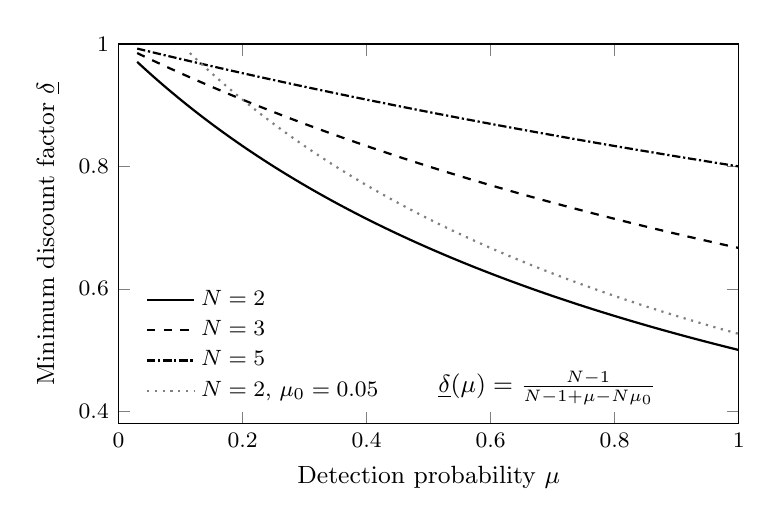
\begin{tikzpicture}
\begin{axis}[
  width=0.78\textwidth, height=6.4cm,
  xmin=0, xmax=1, ymin=0.38, ymax=1.0,
  xlabel={Detection probability $\mu$}, ylabel={Minimum discount factor $\underline{\delta}$},
  tick label style={font=\footnotesize}, label style={font=\small},
  legend pos=south west, legend style={font=\footnotesize, draw=none, fill=white},
  legend cell align=left, samples=200]
\addplot[thick, domain=0.03:1] {1/(1+x)};
\addlegendentry{$N = 2$}
\addplot[thick, dashed, domain=0.03:1] {2/(2+x)};
\addlegendentry{$N = 3$}
\addplot[thick, densely dashdotted, domain=0.03:1] {4/(4+x)};
\addlegendentry{$N = 5$}
\addplot[thick, gray, dotted, domain=0.115:1] {1/(1+x-0.1)};
\addlegendentry{$N = 2$, $\mu_0 = 0.05$}
\node[font=\small, anchor=south west] at (axis cs:0.5,0.395)
  {$\underline{\delta}(\mu) = \frac{N-1}{N-1+\mu-N\mu_0}$};
\end{axis}
\end{tikzpicture}
\caption{The minimum discount factor that sustains collusion at the monopoly price as a function of the
detection probability $\mu$, from \cref{prop:13-transparency} ($\mu_0 = 0$) and \cref{cor:13-false-alarms}
(gray dotted curve, $\mu_0 = 0.05$). With $\mu = 1$ and $\mu_0 = 0$ the threshold is $1 - \frac{1}{N}$.
False alarms shift the curve up, and with $N = 2$ collusion is impossible unless $\mu > 2\mu_0 = 0.1$.}
\label{fig:13-transparency}
\end{figure}

False alarms make collusion harder because they end collusion on the equilibrium path. This lowers the value of
colluding, and with it the loss that a deviator suffers when caught.

\begin{corollary}[False alarms]\label{cor:13-false-alarms}
Under \cref{asm:13-transparency} with $\mu_0 \in [0, \mu)$, the public grim-trigger strategy is a subgame
perfect equilibrium if and only if
\begin{equation}\label{eq:13-false-alarms}
  \delta\,(N - 1 + \mu - N\mu_0) \;\ge\; N - 1 .
\end{equation}
Collusion at $p^m$ is therefore sustainable for some $\delta < 1$ if and only if $\mu > N\mu_0$, and then the
threshold is $\frac{N-1}{N-1+\mu-N\mu_0}$. When $\mu_0 > 0$, collusion on the equilibrium path lasts a geometric
number of periods with mean $\frac{1}{\mu_0}$.
\end{corollary}

\begin{proof}
On the path a false alarm occurs with probability $\mu_0$ each period. The value of collusion solves
$V = \frac{\pi^m}{N} + \delta(1 - \mu_0)V$, so
\begin{equation*}
  V = \frac{\pi^m}{N\left(1 - \delta + \delta\mu_0\right)} .
\end{equation*}
A deviation earns at most $\pi^m$ today and $V$ tomorrow with probability $1 - \mu$. The incentive constraint is
$V \ge \pi^m + \delta(1 - \mu)V$, or $V(1 - \delta + \delta\mu) \ge \pi^m$. Substituting $V$ and multiplying by
$\frac{N(1 - \delta + \delta\mu_0)}{\pi^m}$ gives
\begin{equation*}
  1 - \delta + \delta\mu \;\ge\; N\left(1 - \delta + \delta\mu_0\right)
  \quad\Longleftrightarrow\quad
  \delta\,(N - 1 + \mu - N\mu_0) \;\ge\; N - 1 ,
\end{equation*}
which is \eqref{eq:13-false-alarms}. If $\mu > N\mu_0$, the coefficient on $\delta$ exceeds $N - 1 > 0$, and the
threshold lies below 1. If $\mu \le N\mu_0$, the left side is at most $\delta(N-1) < N - 1$ for every
$\delta < 1$, so no discount factor works. The duration statement follows from \cref{lem:13-durations} with a
per-period exit probability of $\mu_0$.
\end{proof}

\begin{remark}[Relation to Green and Porter]\label{rem:13-gp-nesting}
Set $N = 2$ and $\mu = 1$, and let $\mu_0$ be the probability of a zero-demand period in the Bertrand version of
\citet{GreenPorter1984}. A firm then always sees zero sales after a rival's undercut, and sees zero sales with
probability $\mu_0$ on the path. Condition \eqref{eq:13-false-alarms} becomes $\delta(2 - 2\mu_0) \ge 1$, or
$\delta(1 - \mu_0) \ge \frac{1}{2}$. This is the condition for collusion with permanent reversion in that model
(\cref{ch:collusion-theory}). Profits there are scaled by the probability of positive demand, and the scale
cancels from the incentive constraint. There the optimal cartel shortens punishments to limit the cost of false alarms. The
Sugar Institute lowered $\mu_0$ directly, by verifying accusations before anyone retaliated.
\end{remark}

\begin{remark}[Transparency to buyers]\label{rem:13-transparency-buyers}
Publication informs buyers as well as sellers. Better-informed buyers move faster to a price cutter, which raises
the payoff from a secret cut. Suppose a secret cut captures only a fraction $\omega \in [\frac{1}{N}, 1]$ of the
market, so a deviator earns $\omega\pi^m$. With $\mu_0 = 0$ the incentive constraint becomes
$\frac{\pi^m}{N(1-\delta)} \ge \omega\pi^m + \delta(1-\mu)\frac{\pi^m}{N(1-\delta)}$. The same algebra as in the
proof of \cref{prop:13-transparency} gives
\begin{equation*}
  \delta \;\ge\; \frac{N\omega - 1}{N\omega - 1 + \mu} .
\end{equation*}
This threshold rises with $\omega$ and falls with $\mu$. A policy that raises both $\omega$ and $\mu$ has an
ambiguous effect, so whether transparency raises or lowers prices is an empirical question.
\citet{Stigler1964} made the same point. The more buyers know about prices, the more customers a secret cut
attracts and the faster it is detected. Transparency can also help firms agree on a focal price, as the bromine
firms did when they adopted the trade-journal price after Dow War~I.
\end{remark}

\subsection{Government-assisted coordination: Danish ready-mixed concrete}\label{sec:13-concrete}

\casehead{The question}
\citet{AlbaekMollgaardOvergaard1997} study a natural experiment in transparency. Did the publication of
firm-specific transaction prices by a competition authority lower prices, as the authority intended, or did it
help firms coordinate?

\casehead{The policy}
The Danish Competition Act of 1990 stated its purpose as promoting competition ``through the largest possible
transparency of competitive conditions.'' Unlike U.S.\ and EU law, the Act rested on abuse control. It had no per
se prohibitions, and the authority intervened case by case. A \emph{per se} prohibition makes conduct illegal
without any inquiry into its effects. Under the \emph{rule of reason}, a court weighs the conduct's harm to
competition against its claimed benefits. The Competition Council interpreted the Act to mean
that suspected abuses such as oligopolistic coordination should be countered by more transparency. The premise
was that firm-specific price information lets buyers shop around and so pushes prices down.

\casehead{The product and the market}
Ready-mixed concrete is a mixture of cement, gravel, sand and water, and its strength is measured in megapascals
(MPa). A given grade is homogeneous, and different grades are imperfect substitutes. The study covers a weak grade
(10 MPa), used for foundations of single-family houses, and a strong grade (25 MPa), used for staircases.
Concrete travels in mixer lorries holding at most six cubic metres. It can stay in a lorry for only about two hours,
so it normally travels at most about twenty miles. Denmark had 115 production sites. The two main producers were
Unicon, owned by the only Danish cement producer, and 4K, and the remaining capacity belonged to independent
local firms. In 1987 the national four-firm concentration ratio was 57 percent, with Unicon at 37 percent and 4K
at 11 percent. Two years later Unicon's share reached 43 percent after it acquired the third-largest firm. Within
a radius of 20 km of a plant, many local markets were monopolies, and the average share of the largest firm was
about 70 percent. Typically fewer than five sites could serve a given customer. Pricing combined rigid, publicly
posted list prices with large confidential discounts.

\casehead{The intervention and the data}
In October 1993 the Council decided to sample invoice prices from 18 sites and publish them in its newsletter,
roughly once a quarter. The sites were in three regions, Copenhagen (7 sites), Aarhus (6) and Northern Jutland
(5). For each site and grade the Council published the list price, the average price and the average of the five
lowest prices in the first month of a quarter. Prices appeared with a lag of about three months. The data cover
the four quarters of 1994 and the first three of 1995, seven observations per site. \Cref{tab:13-albaek-timeline}
gives the timeline. The two dominant firms had almost identical list prices in each region. They set the highest
list prices and gave the largest discounts. Average discounts were 25 to 26 percent of list for 10 MPa and 27 to
31 percent for 25 MPa. Maximum discounts ranged from 25 percent in Northern Jutland to 38 percent in Aarhus.

\begin{table}[htbp]
\centering
\caption{Timeline of the Danish concrete price publication}\label{tab:13-albaek-timeline}
\small
\begin{tabular}{@{}ll@{}}
\toprule
Date & Event\\
\midrule
1990 & Competition Act adopts the transparency principle\\
October 1993 & Competition Council decides to collect and publish invoice prices\\
April 8, 1994 & January 1994 prices published\\
July 5, 1994 & April 1994 prices published\\
January to October 1994 & Weighted average price of the two grades rises 19 percent\\
April 1996 & Last publication (November 1995 prices)\\
December 1996 & Council decides to publish no more concrete prices\\
May 30, 1997 & New competition law drops the emphasis on transparency\\
\bottomrule
\end{tabular}

\smallskip
\begin{minipage}{0.8\textwidth}\footnotesize
Notes: From \citet{AlbaekMollgaardOvergaard1997}, pp.~430--433 and 440--441.
\end{minipage}
\end{table}

\casehead{The main finding}
\Cref{fig:13-albaek-f1} shows the national indices of average transaction prices for the two grades, weighted by
the firms' turnover. Prices rose sharply over the first two to three quarters of 1994. According to the Council's
reports, the weighted average increase across the two grades was 19 percent between January and October 1994.
Prices then levelled off. Over the first three quarters of 1994, consumer prices rose 1.9 percent, wholesale
prices 1.6 percent, and import prices of unprocessed raw materials 1.1 percent. An index of residential
construction costs barely moved. The unit value of all concrete produced and the unit value of cement, the main
input, show nothing like the rise in the published prices.

The comparison is a before-after design with an aggregate benchmark. Let $p_t$ be the published price index and
$p^{\mathrm{b}}_t$ a benchmark index that captures costs and general inflation. The implicit estimate of the effect
of publication is
\begin{equation}\label{eq:13-albaek-tau}
  \hat\tau = \left(\ln p_{1} - \ln p_{0}\right) - \left(\ln p^{\mathrm{b}}_{1} - \ln p^{\mathrm{b}}_{0}\right),
\end{equation}
with period 0 in January 1994 and period 1 in October 1994. With a 19 percent price rise and consumer prices as the
benchmark, $\hat\tau \approx \ln 1.19 - \ln 1.019 = 0.155$, or about 17 percent (our computation).
Interpreting $\hat\tau$ as a causal effect requires that, without publication, concrete prices would have moved
with the benchmark. The rest of the paper defends this assumption.

\begin{figure}[htbp]
\centering
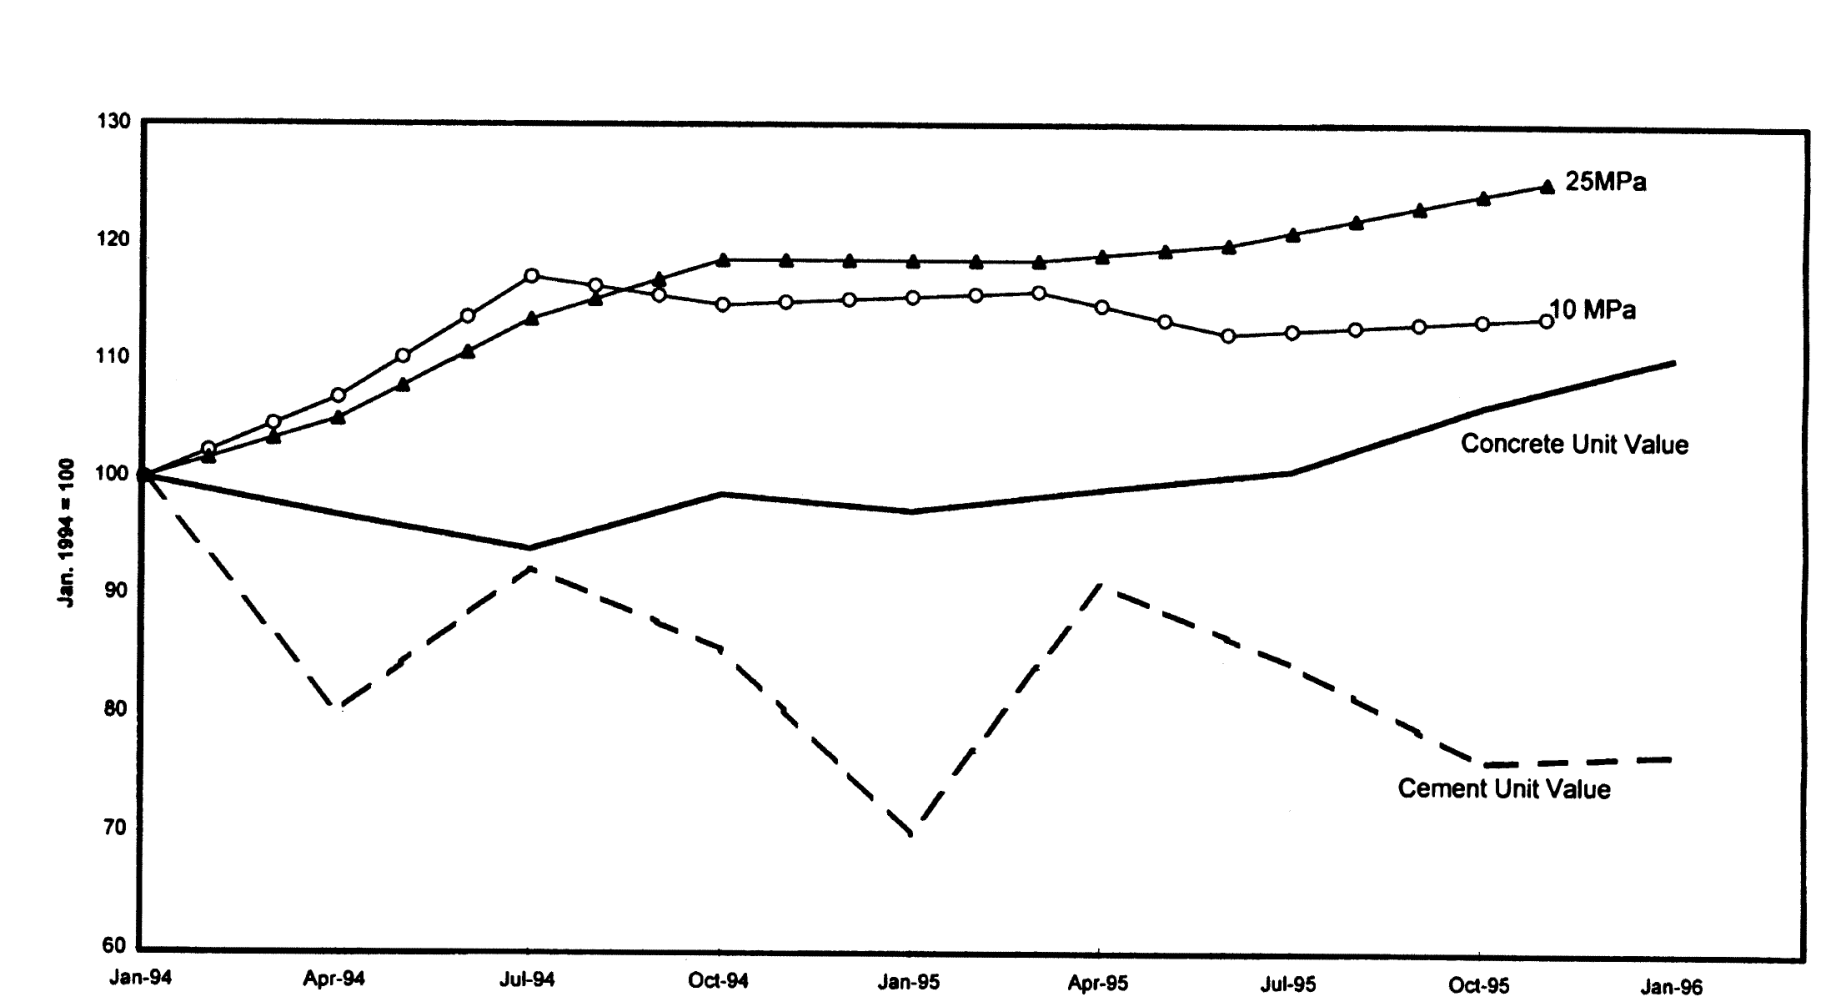
\includegraphics[width=0.88\textwidth]{figures/ch13/albaek1997_fig1.png}
\caption{National price indices for ready-mixed concrete (January 1994 = 100). The marked lines are the published
average transaction prices of 10 MPa and 25 MPa concrete. The solid line is the unit value of all concrete
produced and the dashed line the unit value of cement. Source: \citet{AlbaekMollgaardOvergaard1997}, Figure~1
(unit values from Danmarks Statistik, published prices from the Competition Council).}\label{fig:13-albaek-f1}
\end{figure}

\casehead{Ruling out competitive explanations}
In a price-setting oligopoly with capacity constraints, prices could rise because demand grew, capacity fell or
input prices rose. The authors examine each. A deep construction recession bottomed out in the summer of 1993. By
February 1994 construction employment was back at its low 1992 level. By November 1994 seasonally adjusted
employment had risen 4.4 percent and unadjusted employment 17.6 percent. Production of concrete at the end of 1993
was as low as at the trough ten years earlier. Production in 1994 was almost 20 percent above 1993 but still below
1991.

Capacity was not binding. In 1987 production was more than 50 percent above its 1994 level. Even then, capacity
utilization was about 41 percent in production and 62 percent in distribution, and productive capacity had not
fallen much since. If capacity was unchanged, utilization in 1994 was at most $\frac{62}{1.5} \approx 41$ percent in
distribution and $\frac{41}{1.5} \approx 27$ percent in production (our computation). Distribution capacity is the
number of mixer lorries, which firms could import or move between regions. Input costs did not rise either.
Wages and energy prices were flat from 1993 to 1994, and the unit value of cement fell. The cement supplier, which
owned Unicon, charged uniform delivered prices to all concrete producers.

\casehead{A closer look at Aarhus}
The authors then focus on Aarhus. Its six sampled firms carried about 70 percent of the weight in the national
indices, and price increases in the other two regions were much more moderate. Copenhagen is large, and only half
of its sites were sampled. Northern Jutland is sparsely populated, its sampled firms are local monopolies, and
its discounts were smaller at the outset. Within Aarhus the authors drop a plant on a peninsula more than 60 km
away and a Unicon plant 40 km away in Randers. The remaining four are plants of 4K and Unicon about 2 km apart in
the city, and two commonly owned local plants (Haarup and \O stjysk) 25 km and 40 km away. Together they carried
about 60 percent of the national index weight and had a combined local share close to one.

\begin{figure}[htbp]
\centering
\begin{subfigure}[b]{0.74\textwidth}\centering
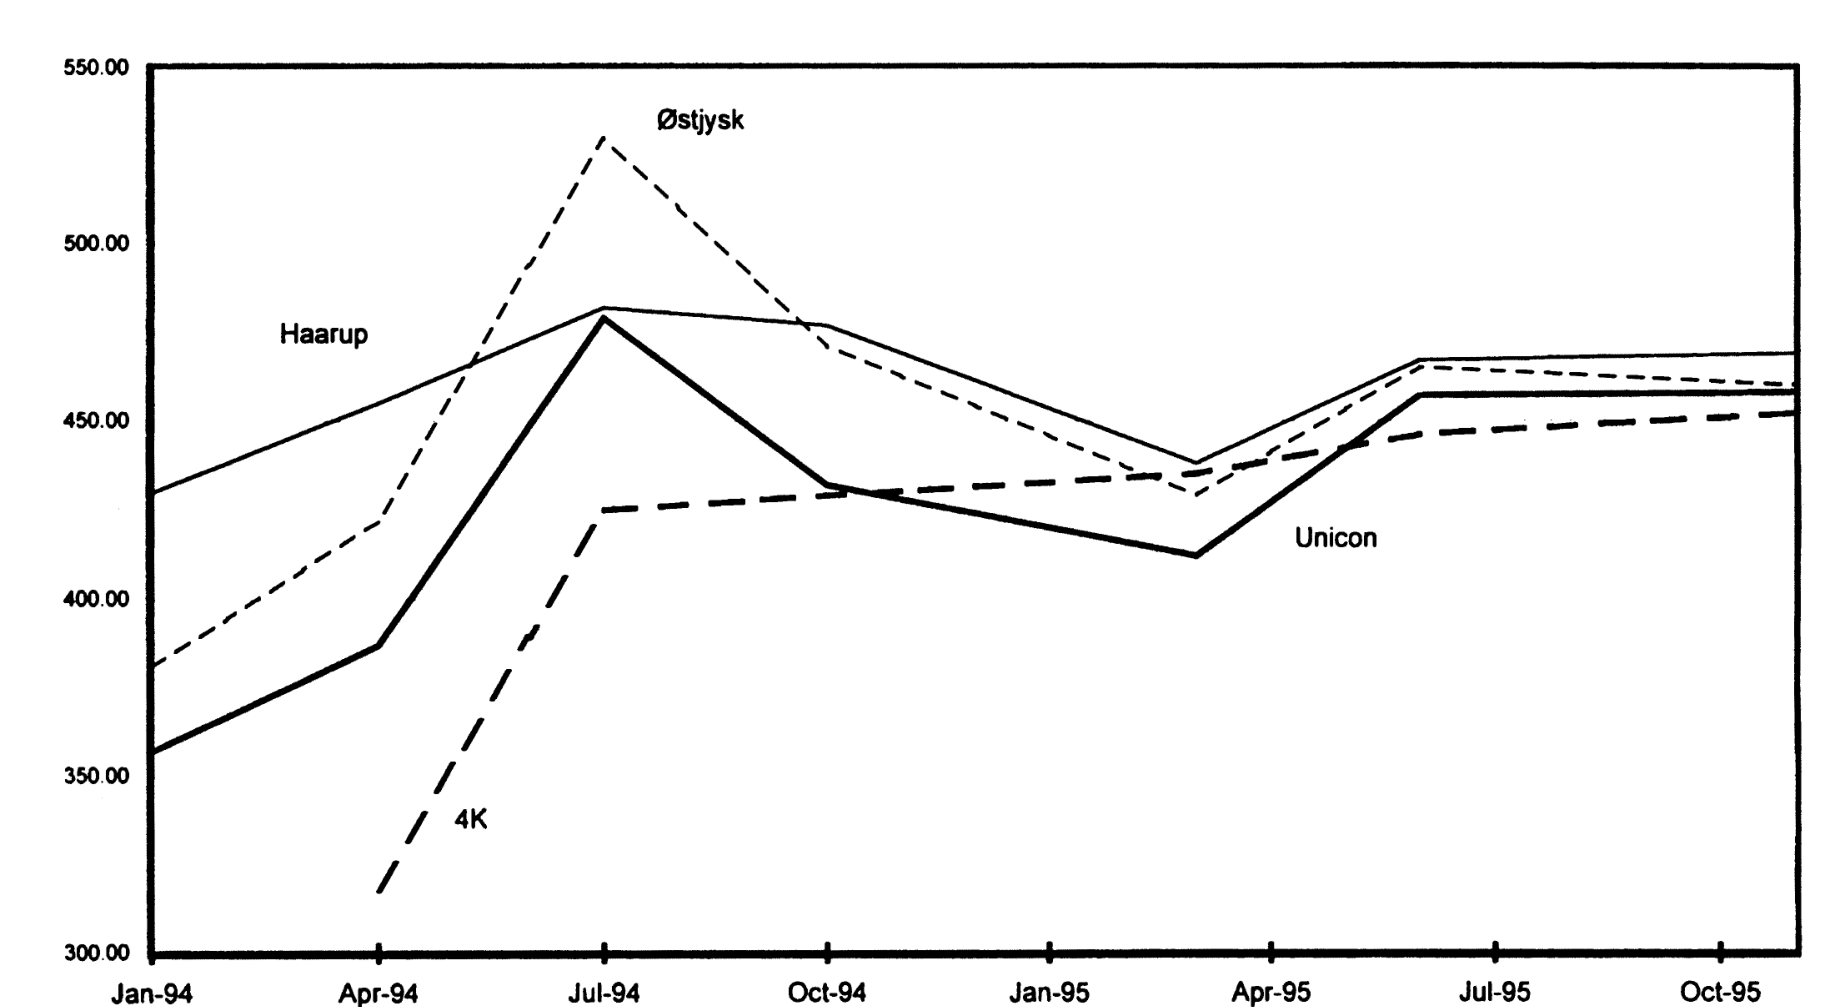
\includegraphics[width=\textwidth]{figures/ch13/albaek1997_fig2.png}
\caption{Figure 2 of the paper}
\end{subfigure}

\medskip
\begin{subfigure}[b]{0.74\textwidth}\centering
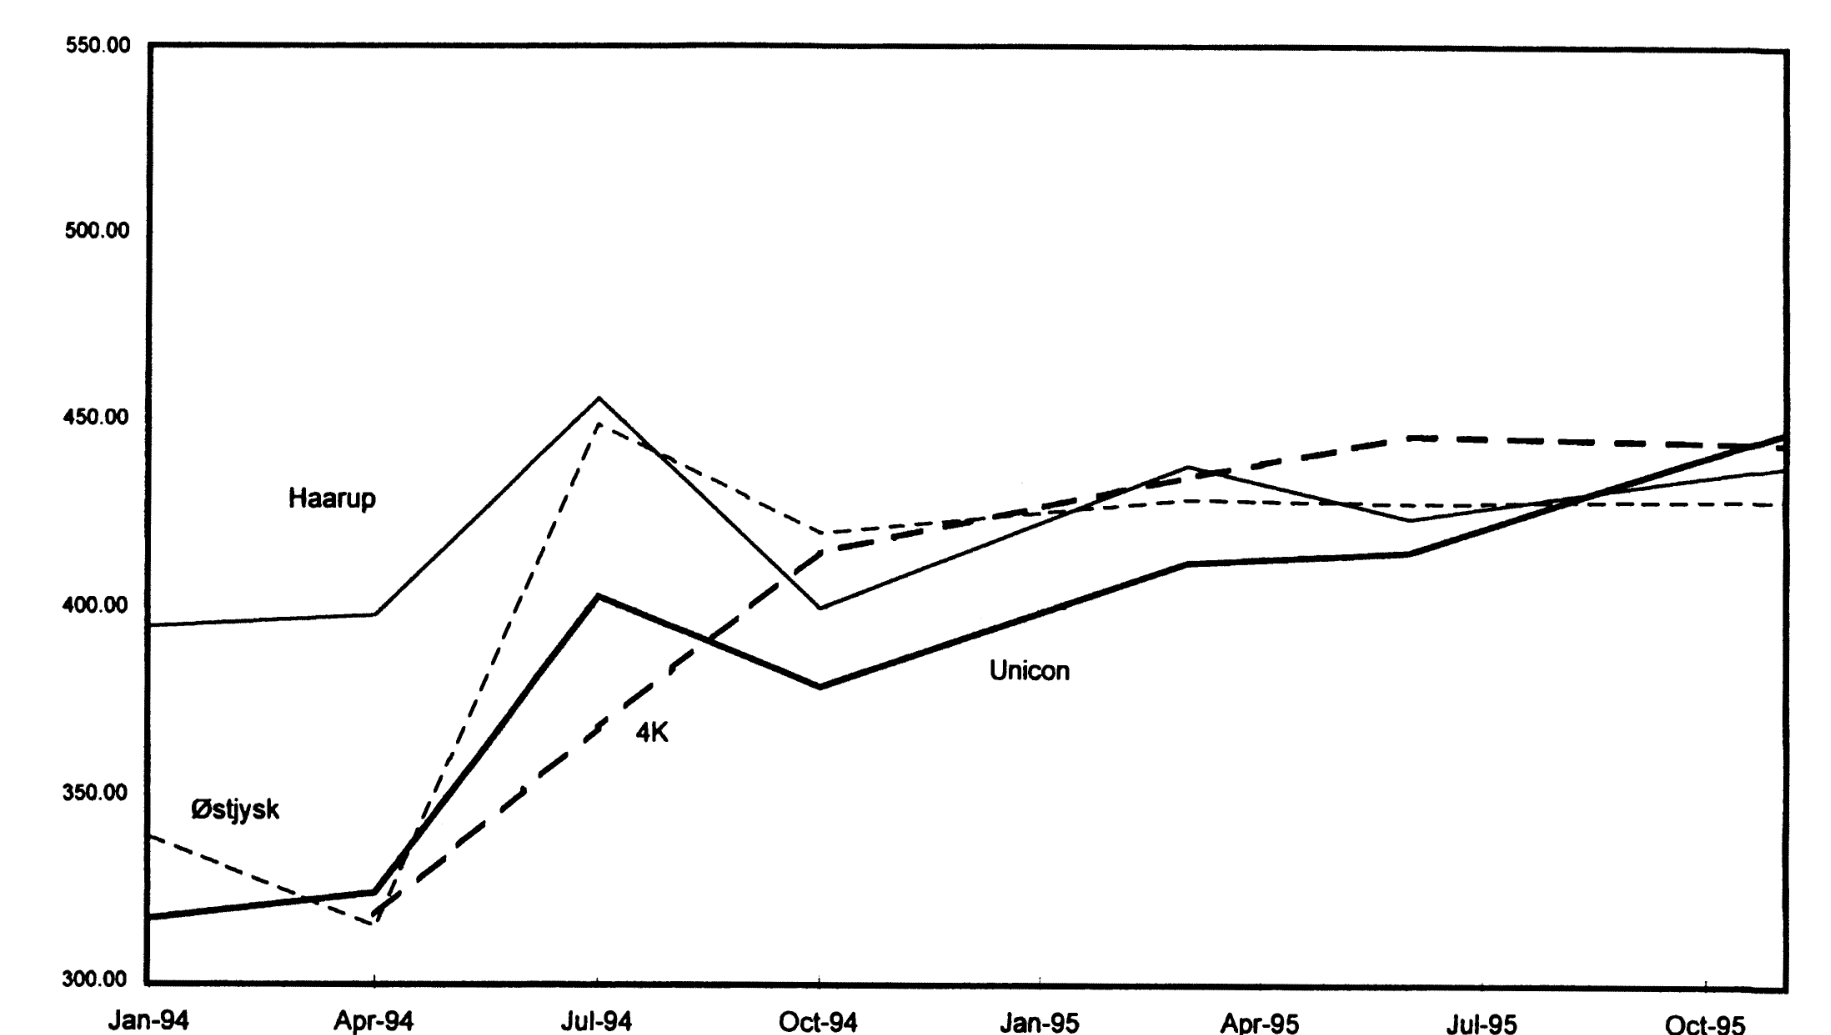
\includegraphics[width=\textwidth]{figures/ch13/albaek1997_fig3.png}
\caption{Figure 3 of the paper}
\end{subfigure}
\caption{Published 10-MPa prices of the four Aarhus plants, January 1994 to October 1995. The journal titles both
panels ``Low 10-MPa Prices in Aarhus.'' The text describes both average and low prices. Panel (b) is flat from
January to April 1994, as the text says of low prices, and lies below panel (a). We therefore read panel (a) as
average prices and panel (b) as low prices. Source: \citet{AlbaekMollgaardOvergaard1997}, Figures~2 and~3 (data from the Competition
Council).}\label{fig:13-albaek-f23}
\end{figure}

\Cref{fig:13-albaek-f23} shows the prices of these four plants. From January to April 1994, low prices were
roughly constant while average prices rose a little. From April to July 1994, prices jumped by 20 to 25 percent and
then stayed at the new level. The timing fits the flow of information. The January prices were published on April
8, 1994, so April transactions could at best partly reflect them. The April prices were published on July 5, so
by July every firm had two quarters of reliable information on rivals' formerly secret discounts. Prices also
converged. By the end of the sample, the four plants' prices varied by only 2 to 4 percent around their mean,
against up to 30 percent early in 1994. Low prices rose toward average prices, so the largest discounts
disappeared. The authors see no explanation for a 25 percent rise in tandem by two major producers 2 km apart,
other than reduced competition after secret discounts became public.

\casehead{Interpretation}
In terms of \cref{prop:13-transparency}, publication raised the detection probability $\mu$ of secret discounts.
The publication lag also mattered for \cref{rem:13-transparency-buyers}. Prices for the first month of a quarter
appeared about three months later. That told each firm what its rivals had charged, but told a buyer little about
the prices it could get today (our reading). The authors ask why a trade association had not supplied the same
information. The association said it received no price reports from members. They suggest that unverified reports
would not be credible, since a firm that gives secret discounts also gains by misreporting. The Council would also
have frowned on industry price reporting (p.~440, fn.~12). The Council itself stopped publishing at the
end of 1996. It noted that the convergence of actual and list prices since January 1994 had come entirely from a
rise in actual prices (p.~430, fn.~4). The authors also point to related evidence from U.S.\ railroad freight.
After Congress mandated the disclosure of firm-specific rail contract terms, grain rates rose.
\citet{FullerRuppelBessler1990} and \citet{SchmitzFuller1995} attribute the rise to the improved scope for
tacit collusion (p.~441).

\casehead{Limitations}
The authors list the main weaknesses. There is no control group, either regions without publication or the same
regions before publication. The Council had some data from before January 1994 but refused access. There are no
data on firms' costs or capacities, and the sample has seven quarterly observations. There is no structural model
and no standard error. One alternative they do not discuss is seasonality. The gap between adjusted and
unadjusted construction employment shows strong seasonal demand, and the jump between April and July coincides with the
building season. A seasonal rise would have reversed, however, and published prices stayed high through 1995
(our observation). Despite its limits, the paper is the cleanest evidence in this chapter that transparency can
raise prices. It also shows that a policy can harm competition through the mechanism of
\cref{prop:13-transparency}.

\subsection{Signaling through a fare-publishing system: the Airline Tariff Publishing case}\label{sec:13-atpco}

\casehead{The question}
Firms may also use an information system to communicate intentions directly. \citet{Miller2010} asks whether an
antitrust case against such communication among U.S.\ airlines changed their prices and output. The airline
industry is described in \cref{ch:airlines}.

\casehead{Setting}
The Airline Tariff Publishing (ATP) Company, owned by the airlines, is the clearinghouse for airline fares. It
collects and disseminates over 100,000 fare updates a day to airlines and to the computer reservation systems of
travel agents. Each entry contains a fare basis code, a dollar amount, a route, fare rules and footnotes, typically
first or last ticket dates. Airlines monitor the updates with sophisticated software. Travel agents can view only
one market at a time and do not see the footnote designators. In December 1992 the Department of Justice sued the
eight major domestic airlines and ATP, alleging that they used the system to communicate and to enforce price
coordination (Civil Action No.~92-2854). The alleged channels were rapid monitoring, enforcement, signaling an
intent to raise fares without shifting market shares \citep{HoltScheffman1987}, bargaining over fares and
restrictions, and linking fares across markets \citep{BernheimWhinston1990,EvansKessides1994}. In a widely cited
example, airlines punished fare cuts by America West with fare codes containing ``HP,'' America West's industry
code, and withdrew them once America West retracted its cuts. The case contrasts with an earlier and blunter
invitation to collude. In 1982 Robert Crandall, chief executive of American Airlines, telephoned Howard Putnam of
Braniff, a rival on routes out of Dallas-Fort Worth. He proposed that Braniff raise its fares by twenty percent and
promised to raise his own the next morning \citep[pp.~188--189]{AskerNocke2021}. Putnam recorded the call and turned
it over to the Department of Justice, which filed a complaint against American and Crandall. Such explicit,
private communication is easy to condemn. The ATP case concerned coded, public signals, which serve the same
purpose and are harder to prohibit (\cref{sec:12-anatomy}).

Without admitting guilt, United and US Airways settled on November 1, 1993, and the other six defendants on August
10, 1994. For ten years the airlines agreed to three restrictions. They would not use footnote indicators or fare basis
codes to convey extraneous information, or special codes linking different fares. They would not preannounce
price changes except for widely publicized sales. A facilitating practice is judged under the rule of reason \citep[p.~570]{Miller2010}, and the airlines
defended ATP as an efficient business tool. \citet{Hay2000} called a related defense ``we're naturally bad.'' It holds
that the industry's rapid monitoring alone explains supracompetitive profits, so restricting ATP would not help.
The theoretical prediction is thus ambiguous.

\casehead{Data}
Miller uses the Department of Transportation's DB1A database, a 10 percent sample of domestic tickets, from the
second quarter of 1991 to the first quarter of 1995. Fares below \$10 (presumed frequent-flyer redemptions) and
above ten times the Standard Industry Fare Level (presumed errors) are dropped, which removes less than 1 percent
of fares. The unit of observation is an airline, city-pair market and quarter. There are 411,726 such cells, with
a mean of 229 sampled tickets and a mean fare of \$209.70. Both vary widely across cells, with standard deviations
of 933.16 tickets and \$129.80, and the mean distance of a market is 1,056 miles (Table~1). The average market has
4.7 airlines, a Herfindahl index of 5,341 points and a four-firm concentration ratio of 97 percent.

\casehead{Design and estimating equation}
The identification strategy compares markets that the case should have affected with markets it should not have
affected. If ATP facilitated collusion among the defendants, the remedy should matter only where several
defendants compete. \emph{Affected} markets are city pairs served by more than two defendant airlines in every
quarter. \emph{Control} markets are city pairs where the number of major airlines is always below two. Let
$Y_{ijt}$ be tickets sold or the average fare of airline $i$ in city pair $j$ in quarter $t$. Let
$\mathit{ATP1}_t$ equal one from the second quarter of 1992, after the investigation intensified with the first
depositions in March 1992. Let $\mathit{ATP2}_t$ equal one from the first quarter of 1994, after the settlements
began. The probe itself had been announced in June 1990, and Miller dates the treatment from its intensification.
An event study finds no response of defendants' stock prices to the 1990 announcement and a significant negative
response to the intensification on March 18, 1992 (p.~574, note~9). The estimating equation is
\begin{equation}\label{eq:13-miller-did}
  Y_{ijt} = \beta_0 + \sum_{k=1}^{2}\beta_{k}^{A}\,\mathit{ATPk}_t\cdot\mathit{Aff}_j
          + \sum_{k=1}^{2}\beta_{k}\,\mathit{ATPk}_t + x_{jt}\beta_X + a_i + g_j + e_{ijt} .
\end{equation}
Here $\mathit{Aff}_j$ marks affected markets, and $a_i$ and $g_j$ are airline and city-pair fixed effects. The
controls $x_{jt}$ are the Standard Industry Fare Level, a cost measure, and the geometric means of the endpoint
states' populations and gross state products, which shift demand. Richer versions replace $\beta_k\mathit{ATPk}_t$
with quarter effects or with airline-by-quarter effects. Standard errors are clustered by city pair.

The two indicators are cumulative steps. The coefficient $\beta^{A}_1$ is the effect during the investigation, and
$\beta^{A}_1 + \beta^{A}_2$ is the effect after the settlement. A lasting effect of the remedy requires
$\beta^{A}_1 + \beta^{A}_2 \neq 0$, which Miller tests with an $F$ test. Identification rests on parallel trends.
Affected and control markets would have evolved alike absent the case, conditional on the controls. The model is
identified even with airline-by-quarter effects, because each airline serves both kinds of market before and after
the case. Affected and control markets differ in fares and distance. Miller therefore repeats the analysis with a second
control group of dominated markets, in which one airline sells over 90 percent of tickets in every quarter.

Miller also checks the results on several restricted samples (pp.~575--577). They keep flights within the
continental United States, markets with distances between 250 and 2,000 miles, and markets with stable numbers of
defendant and other airlines. One restriction counts an airline as present only if it has at least 10 sampled
tickets in the market, about 100 passengers a quarter. Another reassigns the tickets of commuter carriers to the
defendants with which they had operating agreements (p.~577, note~14). Combining all of these restrictions leaves
736 city-pair markets, the sample of columns (3) and (6) of \cref{tab:13-miller-t2}.

\begin{table}[htbp]
\centering
\caption{Quantity and price effects of the Airline Tariff Publishing case}\label{tab:13-miller-t2}
\small
\begin{tabular}{@{}lcccccc@{}}
\toprule
 & \multicolumn{3}{c}{Number of tickets} & \multicolumn{3}{c}{Average fare (dollars)}\\
\cmidrule(lr){2-4}\cmidrule(l){5-7}
 & (1) & (2) & (3) & (4) & (5) & (6)\\
\midrule
Quarter fixed effects & No & Yes & Yes & No & Yes & Yes\\
Airline $\times$ quarter effects & No & No & Yes & No & No & Yes\\
Sample restrictions & No & No & Yes & No & No & Yes\\
\addlinespace
$\mathit{ATP1}$ & 105.194 & & & 1.595 & & \\
 & (43.039) & & & (2.654) & & \\
$\mathit{ATP2}$ & 66.433 & & & $-10.746$ & & \\
 & (55.741) & & & (2.517) & & \\
$\mathit{ATP1}\times\mathit{Aff}$ & $-91.983$ & $-92.425$ & $-4.361$ & $-13.568$ & $-14.085$ & $-7.051$\\
 & (43.164) & (43.081) & (18.697) & (2.680) & (2.661) & (2.270)\\
$\mathit{ATP2}\times\mathit{Aff}$ & $-40.318$ & $-41.081$ & $-59.948$ & 12.708 & 14.619 & 2.932\\
 & (56.013) & (55.990) & (20.977) & (2.598) & (2.152) & (2.616)\\
\addlinespace
p-value, $(\mathit{ATP1} + \mathit{ATP2})\times\mathit{Aff} = 0$ & 0.08 & 0.08 & 0.05 & 0.81 & 0.86 & 0.17\\
$N$ & 328{,}921 & 328{,}921 & 10{,}934 & 328{,}921 & 328{,}921 & 10{,}934\\
City-pair markets & 4{,}825 & 4{,}825 & 736 & 4{,}825 & 4{,}825 & 736\\
$R^2$ & 0.05 & 0.05 & 0.22 & 0.04 & 0.05 & 0.34\\
\bottomrule
\end{tabular}

\smallskip
\begin{minipage}{0.95\textwidth}\footnotesize
Notes: Reproduced from \citet{Miller2010}, Table~2. The unit is an airline, market and quarter in the
10 percent ticket sample. All regressions include city-pair and airline fixed effects and the controls described
in the text. Standard errors clustered by city pair in parentheses. Columns (3) and (6) combine the sample
restrictions listed in the text, which leave 736 markets.
\end{minipage}
\end{table}

\casehead{Results}
\Cref{tab:13-miller-t2} reproduces the main estimates. Tickets rose in affected markets after the case, but they
rose more in control markets. In column (1) the relative change after the settlement is
$-91.983 - 40.318 = -132.3$ sampled tickets per airline, market and quarter, significant at the 8 percent level.
Multiplying by 10 to undo the sampling gives about 1,300 tickets, the ``over 1,000 tickets per quarter'' in the
text (our reconstruction). Column (3) gives $10 \times (4.361 + 59.948) = 643$, matching the reported
postsettlement decline of 640 tickets, significant at the 5 percent level. Lower relative traffic contradicts a
lasting increase in competition and fits the airlines' claim that the restrictions made travel planning harder.

Fares fell and then recovered. In column (4), affected-market fares fell \$13.57 relative to control markets
during the investigation and rose \$12.71 after the settlement. The net effect of $-\$0.86$ is insignificant
($p = 0.81$). With the average fare near \$210, the initial fall is about 6.5 percent (our computation). In logs,
the two coefficients are $-0.088$ and $0.035$, both significant. The pattern holds across the fare distribution.
With quarter effects, the investigation lowered the 10th percentile, median and 90th percentile fares by \$9.08,
\$10.98 and \$28.93, and the settlement raised them by \$9.51, \$14.76 and \$21.24 (Table~3). Price dispersion
therefore fell and then rose, and only the 90th percentile shows a net decline, significant at the 10 percent
level.

\begin{figure}[htbp]
\centering
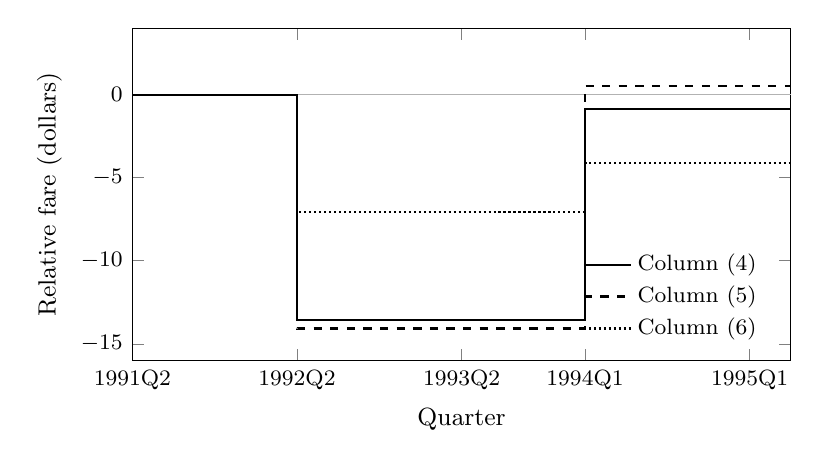
\begin{tikzpicture}
\begin{axis}[
  width=0.82\textwidth, height=5.8cm,
  xmin=1991.25, xmax=1995.25, ymin=-16, ymax=4,
  xlabel={Quarter}, ylabel={Relative fare (dollars)},
  xtick={1991.25,1992.25,1993.25,1994.0,1995.0},
  xticklabels={1991Q2,1992Q2,1993Q2,1994Q1,1995Q1},
  tick label style={font=\footnotesize}, label style={font=\small},
  legend pos=south east, legend style={font=\footnotesize, draw=none, fill=none}, legend cell align=left]
\draw[gray!60] (axis cs:1991.25,0) -- (axis cs:1995.25,0);
\addplot[thick, const plot] coordinates {(1991.25,0) (1992.25,-13.568) (1994.0,-0.860) (1995.25,-0.860)};
\addlegendentry{Column (4)}
\addplot[thick, dashed, const plot] coordinates {(1991.25,0) (1992.25,-14.085) (1994.0,0.534) (1995.25,0.534)};
\addlegendentry{Column (5)}
\addplot[thick, densely dotted, const plot] coordinates {(1991.25,0) (1992.25,-7.051) (1994.0,-4.119) (1995.25,-4.119)};
\addlegendentry{Column (6)}
\end{axis}
\end{tikzpicture}
\caption{Average fares in affected markets relative to control markets implied by
\citet{Miller2010}, Table~2. The path is 0 before the second quarter of 1992, $\beta^{A}_1$ during the
investigation, and $\beta^{A}_1 + \beta^{A}_2$ from the first quarter of 1994. Our construction from the reported
coefficients.}\label{fig:13-miller-path}
\end{figure}

\Cref{fig:13-miller-path} plots the implied fare paths. Two further results support the reading of a temporary
effect. Separate regressions for defendants and other airlines show that the fall and rise in fares came from the
defendants, whose relative fares fell \$8.71 and then rose \$10.49 (Table~4). Their relative ticket sales rose
during the investigation, while other airlines lost traffic. The defendants' fare cuts mostly shifted passengers
from other carriers. Miller also re-estimates the multimarket-contact regression of \citet{EvansKessides1994}:
\begin{equation}\label{eq:13-miller-mmc}
  \ln \mathit{Price}_{ijt} = x_{ijt}\beta_X + \beta_Z Z_{jt} + \sum_{k=1}^{2}\beta_{Zk}\,\mathit{ATPk}_t\cdot Z_{jt}
    + a_i + g_j + \tau_t + e_{ijt} .
\end{equation}
Here $Z_{jt}$ is the average number of routes that the airlines serving market $j$ have in common, divided by
1,000. The controls $x_{ijt}$ include the airline's route and airport shares and the route Herfindahl index. In the
Evans-Kessides sample, the contact coefficient is 0.269 (0.043). It falls by 0.104 (0.030) during the
investigation and rises by 0.107 (0.033) after the settlement, with a p-value of 0.96 for no net change
(Table~5). In this sample the contact effect weakened while the case was active, to $0.269 - 0.104 = 0.165$, or
about three fifths of its initial value. After the settlement it rose to $0.165 + 0.107 = 0.272$, close to its
initial value. The p-value concerns the net change,
so it says nothing about whether the coefficient of 0.165 differs from zero. In the two larger samples the
interaction largely offsets the baseline coefficient, $0.016 - 0.014$ and $0.035 - 0.025$, and Miller reports that
contact was then an insignificant predictor of prices (p.~582). Finally, the hub premium,
which should have risen if collusion in contested markets broke down, fell by about 8 percent during the
investigation and by another 13 percent after the settlement.

\casehead{Interpretation and critiques}
The defendants lowered fares under the scrutiny of the investigation and raised them once the settlement was in
place. The settlement left the system largely intact, including the rapid fare monitoring that lets airlines
detect and match fare cuts. In terms of \cref{prop:13-transparency}, the remedy removed some signaling devices but
left the detection probability $\mu$ high. The business press described weekend fare changes as a near substitute
for the forbidden preannouncements. American Airlines was later accused of violating the decree and accepted a
new seven-year decree in 2004. Alternatively, the airlines may never have used ATP as alleged.
\citet{Borenstein2004} reports relative price increases after the settlement on 387 routes likely to be affected,
consistent with Miller.

The design has weaknesses that Miller discusses. Group membership depends on entry and exit, which are outcomes.
She treats it as predetermined over four years and drops markets whose group changes. Southwest's entry was more
frequent in affected markets, and the results survive dropping markets that Southwest entered or left. Affected
and control markets differ in fares, distances and traffic, which weakens parallel trends, so she repeats the
analysis with dominated markets as controls. The timing of treatment is also uncertain. The probe was announced in
June 1990, the suit filed in December 1992, and the settlements signed in 1993 and 1994. The paper does not report
pre-trends, so the identifying assumption cannot be checked directly (our observation). The case connects to the
retrospective methods of \cref{sec:13-enforcement}. Miller reads the time pattern of fares as a sign that the
settlement failed because of its limited scope, and she rejects the reading that the industry was already
competitive (p.~570). She also warns that a weak settlement can be empirically indistinguishable from one applied
to an already competitive industry (p.~573). The pattern is consistent with a remedy that removed signaling devices
while leaving rapid fare monitoring and other coordination channels intact. The design does not separately identify
these channels.

\subsection{Rules among nonprofits: the Overlap group and financial aid}\label{sec:13-overlap}

\casehead{The question}
Can an agreement on rules among nonprofit institutions raise prices? \citet{CarltonBambergerEpstein1995} study the
antitrust case against the Overlap group of universities. They ask whether the schools' agreement on financial aid
raised the average price that students paid. They also ask how antitrust law should treat collective action by
nonprofits. The study grew out of work by Lexecon for MIT, and Carlton testified as MIT's expert witness, as the
paper discloses.

\casehead{The agreement}
In the 1950s the Ivy League schools met to stop bidding for star athletes. They agreed that no athlete would
receive aid beyond financial need, and soon applied the same idea to star students. By the 1970s the Overlap
meetings included the eight Ivy League schools, MIT and 14 other selective colleges, 23 schools in all. Their
combined undergraduate enrollment of about 60,000 was less than one percent of the national total.
\Cref{fig:13-cbe-aid} shows the accounting. Let $\bar p$ be the gross charge for tuition, room, board and fees. A
student covers it with grants $G$, self help $H$ (loans and jobs) and a family contribution $F$. In this subsection
$G$, $H$ and $F$ are local symbols for these three sources, not distribution functions:
\begin{equation}\label{eq:13-cbe-accounting}
  \bar p = G + H + F, \qquad \text{aid package} = G + H, \qquad \text{payment to the school} = H + F = \bar p - G .
\end{equation}
The Overlap schools agreed to give aid only on the basis of need and to use a common method to define need. They
also met to discuss individual students admitted by more than one school. A printout of commonly admitted students
listed each school's proposed family contribution. When proposals differed by more than several hundred dollars,
the schools discussed them and usually agreed on a common figure. Disagreements arose for 10 to 20 percent of the
commonly admitted students who applied for aid. Regardless of which Overlap school admitted a student, the family
contribution $F$ was the same. Some schools also agreed on the split of the aid package between $H$ and $G$.

\begin{figure}[htbp]
\centering
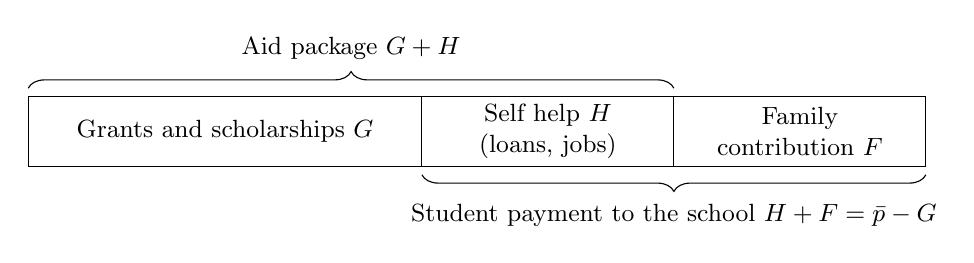
\begin{tikzpicture}[font=\small]
\draw (0,0) rectangle (5,0.9) node[pos=0.5, align=center] {Grants and scholarships $G$};
\draw (5,0) rectangle (8.2,0.9) node[pos=0.5, align=center] {Self help $H$\\(loans, jobs)};
\draw (8.2,0) rectangle (11.4,0.9) node[pos=0.5, align=center] {Family\\contribution $F$};
\draw[decorate, decoration={brace, amplitude=6pt}] (0,1.0) -- (8.2,1.0)
  node[midway, above=7pt] {Aid package $G + H$};
\draw[decorate, decoration={brace, amplitude=6pt, mirror}] (5,-0.1) -- (11.4,-0.1)
  node[midway, below=7pt] {Student payment to the school $H + F = \bar p - G$};
\end{tikzpicture}
\caption{The components of the gross charge $\bar p$ for a student receiving aid. The Overlap schools agreed on the
family contribution $F$ of commonly admitted aid applicants. Redrawn from \citet{CarltonBambergerEpstein1995},
Figure~1.}\label{fig:13-cbe-aid}
\end{figure}

The schools justified the agreement as a way to concentrate scarce aid on needy students, supporting need-blind
admission with a guarantee of full aid for every admitted student. Few schools outside Overlap made both
commitments. Federal aid policy had the same logic, since federal money generally goes only to needy students.

\casehead{The case}
In 1991 the Antitrust Division sued MIT and the eight Ivy League schools under Section~1 of the Sherman Act. It
called the agreement ``garden variety price fixing'' on the number and size of discounts from list price. By
limiting discounts, it claimed, the schools raised the prices paid by meritorious high-income students and the
average price paid by all. There was no allegation that enrollment fell, and enrollment growth at Overlap and
non-Overlap private schools was similar in 1984--1990. The Government asked for per se condemnation. The Ivy League
schools signed a consent decree, and MIT went to trial. In July 1992 Congress passed the Higher Education Act
of 1992. It gave prospective antitrust immunity to much Overlap-type conduct but not to discussions of individual
students. In September 1992 the District Court found MIT guilty of price fixing. In September 1993 the Court of
Appeals overturned the
verdict and ordered a full rule-of-reason analysis that weighed the social benefits claimed by MIT. In December 1993
the Government settled. MIT and other schools could agree not to give merit aid, use common principles to assess
need, pool student information and audit departures, but could not discuss individual awards.

\casehead{Theory}
The authors argue that the Government's claim that average prices must rise is wrong as a matter of theory for
nonprofits. A university's objective has many attributes, including the quality of education, the welfare of
students, faculty and administrators, research, innovation and donors' preferences. At MIT, student charges covered
only about half the full cost of education. Schools erect barriers to trade that a profit maximizer would not. They
do not sell admission, and the authors suspect that Harvard or MIT could profitably auction its last five places.
Raising the average price would raise revenue for valued uses but would harm students, who are part of the
objective. The authors also ask why schools colluding to raise revenue would target needy students rather than
rich ones, and why they would keep need-blind admission. These facts raise doubts but cannot rule out a price
effect, so the question is empirical.

The accounting identity \eqref{eq:13-cbe-accounting} shows what the data can test. Let $n$ students attend a
school and let $G_s$ be student $s$'s institutional grant. Average net revenue per student is
\begin{equation}\label{eq:13-cbe-avg}
  p = \bar p - \frac{1}{n}\sum_{s=1}^{n} G_s .
\end{equation}
The Government's theory implies that Overlap lowered total grants $\sum_s G_s$ and so raised $p$. The schools'
theory implies that Overlap reallocated grants from merit to need, changing the distribution of $G_s$ without
changing their sum. Average net price $p$ discriminates between the two theories. It is silent on how the
agreement redistributed aid.

\casehead{Data}
A before-and-after comparison is infeasible. Overlap had met for over 30 years, and it stopped after the 1991--1992
academic year, leaving only two years of data contaminated by the lawsuit. The authors therefore compare schools.
The 23 Overlap schools fall into five 1987 Carnegie classifications, and annual data for 1984--1990 cover about 225
private and public schools in these classes. The dependent variable is the real average price per student. It equals gross
tuition plus room and board plus mandatory fees minus the average institutionally administered grant per student,
deflated to 1990 dollars by the consumer price index. Institutional grants are the school's own money plus small
federal SEOG grants of about \$50 per undergraduate. For the 162 private schools in the pooled sample, the average
net price is \$12,366 with a standard deviation of \$2,420 (Table~4).

The regressors in their Table~2 are an Ivy-plus-MIT Overlap dummy $\mathit{IVY}$ and an other-Overlap dummy
$\mathit{NONIVY}$. Carnegie dummies are $\mathit{RSRCH1}$, $\mathit{RSRCH2}$, $\mathit{DOCTOR1}$ and
$\mathit{DOCTOR2}$, with Liberal Arts~I omitted. Quality is measured by the percent of applicants accepted
($\mathit{PCTACC}$), the percent scoring above 700 on the verbal or mathematics SAT ($\mathit{SAT}$) and the
percent completing a degree ($\mathit{COMPDEG}$). Financial capacity is measured by real endowment per
full-time-equivalent student in thousands ($\mathit{ENDOW}$) and by the percent of students not receiving
need-based aid ($\mathit{PCTNOAID}$, a wealth proxy). Real state per capita disposable income ($\mathit{YDPC}$)
proxies both income and costs. Further dummies mark non-religious schools ($\mathit{NONRELIG}$), public schools
($\mathit{PUBLIC}$) and missing fee data ($\mathit{FEEMISS}$).

\casehead{Estimating equations}
For school $i$ in year $t$, the annual cross-section model is
\begin{equation}\label{eq:13-cbe-annual}
  p_{it} = x_{it}\beta_t + e_{it},
\end{equation}
estimated separately for each year by least squares. Here $i$ indexes schools, a local use. Because the regressors
change slowly within a school, a pooled regression essentially uses cross-school variation. The authors
therefore also estimate a school-average model. Let $N_i$ be the number of years with data for school $i$ and let
$d_{it} = \frac{1}{N_i}$ for those years. Averaging \eqref{eq:13-cbe-annual} with a common $\beta$ gives
\begin{equation}\label{eq:13-cbe-average}
  \bar p_i = \sum_t d_{it}p_{it} = \Big(\sum_t d_{it}x_{it}\Big)\beta + \sum_t d_{it}e_{it} .
\end{equation}
If the $e_{it}$ are uncorrelated over time with common variance $\sigma^2$, the averaged error has variance
$\Var\big(\sum_t d_{it}e_{it}\big) = \frac{\sigma^2}{N_i}$. Multiplying \eqref{eq:13-cbe-average} by
$\sqrt{N_i}$ makes the error homoskedastic, and least squares on the transformed equation is generalized least
squares. This is why the authors weight by $\sqrt{N_i}$ (WP p.~19, fn.~22). They also report White standard errors,
which are similar.

\begin{table}[htbp]
\centering
\caption{Determinants of the average net price per student at private colleges}\label{tab:13-cbe-t6}
\small
\begin{tabular}{@{}lcc@{\hspace{2.2em}}lcc@{}}
\toprule
\multicolumn{6}{@{}l}{\textit{Panel A. School averages, 1984--1990, weighted by $\sqrt{N_i}$ (Table 6)}}\\
\midrule
Variable & Coef. & (s.e.) & Variable & Coef. & (s.e.)\\
\midrule
Intercept & 2299.47 & (2429.07) & $\mathit{PCTACC}$ & $-27.89$ & (11.97)\\
$\mathit{IVY}$ & $-322.42$ & (678.72) & $\mathit{PCTNOAID}$ & 43.58 & (9.44)\\
$\mathit{NONIVY}$ & 130.37 & (463.81) & $\mathit{SAT}$ & 2.31 & (11.16)\\
$\mathit{RSRCH1}$ & 1042.21 & (435.09) & $\mathit{YDPC}$ & 0.36 & (0.07)\\
$\mathit{RSRCH2}$ & 1062.57 & (514.05) & $\mathit{COMPDEG}$ & 45.68 & (16.64)\\
$\mathit{DOCTOR1}$ & 545.66 & (551.02) & $\mathit{NONRELIG}$ & 1343.18 & (250.19)\\
$\mathit{DOCTOR2}$ & $-1143.27$ & (493.21) & $\mathit{ENDOW}$ & $-5.95$ & (3.77)\\
$\mathit{FEEMISS}$ & $-540.82$ & (294.78) & Observations & \multicolumn{2}{c}{162}\\
\midrule
\multicolumn{6}{@{}l}{\textit{Panel B. Overlap coefficients in the annual regressions (Table 5)}}\\
\midrule
 & 1984 & 1985 & 1986 & 1987 & 1989\\
\midrule
$\mathit{IVY}$ & 271.84 & 21.92 & 4.14 & 16.87 & $-918.91$\\
 & (714.52) & (788.16) & (762.04) & (882.56) & (1079.05)\\
$\mathit{NONIVY}$ & 120.53 & 172.84 & 173.84 & 688.30 & 161.56\\
 & (468.39) & (529.46) & (517.53) & (658.66) & (650.61)\\
$N$ & 130 & 137 & 136 & 106 & 105\\
\bottomrule
\end{tabular}

\smallskip
\begin{minipage}{0.95\textwidth}\footnotesize
Notes: Reproduced from \citet{CarltonBambergerEpstein1995}, NBER working-paper version, Tables~5 and~6.
Dependent variable: real gross tuition, room, board and mandatory fees minus the average
institutional grant per student, in 1990 dollars. Standard errors in parentheses. Panel B also has a 1990
column, with $\mathit{IVY}$ $-2.22$ (1681.46), $\mathit{NONIVY}$ 422.67 (1092.78) and $N = 53$. No Ivy Overlap
school reported complete data for 1988.
\end{minipage}
\end{table}

\casehead{Results}
\Cref{tab:13-cbe-t6} reproduces the results for private schools. In no annual regression is either Overlap
coefficient positive and significant. In the pooled average regression, $\mathit{IVY}$ is $-322$ dollars with a
standard error of 679, and $\mathit{NONIVY}$ is 130 dollars with a standard error of 464. If anything, Overlap
schools charged less, though not significantly so. With gross charges as the dependent variable, the Overlap
coefficient is $-376$ dollars and insignificant (fn.~24). The authors also display the fit school by school
(their Figures~2 and~3). Equation \eqref{eq:13-cbe-average} overpredicts the average price of four of the seven
Ivy-plus-MIT schools with data and underpredicts it for the other three. Their residuals are small and average
close to zero. The other coefficients are sensible. Schools with richer
students charge more, and non-religious schools charge about \$1,500 more than religious ones in the annual
regressions.
Including public schools gives about 225 schools and a significant public-school effect of about $-\$8{,}400$.

The quality premium is modest. Compare a selective school ($\mathit{PCTACC} = 25$, $\mathit{COMPDEG} = 80$) with a
less selective one ($\mathit{PCTACC} = 75$, $\mathit{COMPDEG} = 40$). The predicted difference is
\begin{equation*}
  -27.89\,(25 - 75) + 45.68\,(80 - 40) = 1{,}394.5 + 1{,}827.2 = 3{,}222 \text{ dollars}
\end{equation*}
(our computation), the ``roughly \$3000'' of the text and about a quarter of the average price. The authors compare
it with the return to an elite education. \citet{JamesEtAl1989} find that graduates of elite schools earn 3 to 5
percent more. With a base income of \$50,000, a 5 percent premium and a 10 percent real interest rate, the premium
is worth about $\frac{0.05 \times 50{,}000}{0.10} = 25{,}000$ dollars as a perpetuity.

\casehead{Robustness}
The finding survives several checks. Generalized least squares on the panel with equicorrelated errors within a
school gives a correlation of about 0.8 and results like those in \cref{tab:13-cbe-t6}. A random-effects model
cannot be distinguished from a fixed-effects model by a \citet{Hausman1978} test. The fixed-effects model cannot
identify the Overlap effect, but its other coefficients match. Results are unchanged with public schools
included, with suspect duplicate observations dropped, with quadratic terms in $\mathit{PCTACC}$,
$\mathit{COMPDEG}$ and $\mathit{ENDOW}$, and with logs. Dropping the wealth variable, which is the regressor most
likely to be endogenous, or lagging it, leaves the Overlap coefficients unchanged. To address the endogeneity of
Overlap membership itself, the authors estimate the model on non-Overlap schools only and test whether it fits the
excluded schools. An $F$ test never rejects, and the model predicts the Overlap schools' average prices well.

\casehead{The case for collective action}
The authors argue that without Overlap, competition for star students would have diverted aid from needy to
meritorious students. Merit aid was growing as a share of institutional aid. Across 72 schools, the ratio of merit
aid to need aid rose from 0.134 in 1984 to 0.180 in 1989, and among Liberal Arts~I colleges from 0.076 to 0.131
(Table~7). To test whether Overlap raised access, they regress the log odds of the black or Hispanic share of
students on the same variables (Table~8). One regressor is added, the state's minority share of the college-age
population. For black
students the Overlap coefficient is 0.451 (0.172). Splitting it, $\mathit{IVY}$ is 0.396 (0.268) and
$\mathit{NONIVY}$ 0.478 (0.198). For Hispanic students the coefficient is 0.183 (0.146), with $\mathit{IVY}$ 0.025
(0.227) and $\mathit{NONIVY}$ 0.258 (0.167). A log-odds effect of 0.451 raises a 3 percent share to
$\frac{0.0309 \times e^{0.451}}{1 + 0.0309 \times e^{0.451}} = 4.6$ percent (our computation), close to the
authors' ``about five rather than about three percent.'' They note that Overlap schools may simply have recruited
black students harder.

The Court of Appeals distinguished the case from \textit{National Society of Professional Engineers},
where the Supreme Court struck down a quality-motivated bidding restriction by an association of profit-maximizing
members. It noted ``the absence of any finding of adverse effects such as higher price or lower output'' and that
the agreement was not intended to raise revenue. The authors support this reasoning. Institutions granted
501(c)(3) status pursue social goals that competition among profit maximizers does not achieve. If such goals
could never justify collective action, no collective action by nonprofits would be legal.

\casehead{Critiques}
Identification is by selection on observables in a cross-section. Overlap membership is not random, and
the Ivy-plus-MIT coefficient rests on seven schools with data (Dartmouth and Cornell are missing), all at the
extremes of selectivity and wealth. Some controls may themselves respond to Overlap. The share of students not
receiving need-based aid, $\mathit{PCTNOAID}$, depends on aid policy, and conditioning on it can absorb part of the
effect being measured (our observation). The test concerns the mean of the price distribution, while the
schools' own account implies a change in its shape, a transfer from meritorious high-income students to others.
The authors' conclusion says exactly this. Finally, the test has limited power. The 95 percent confidence interval
for $\mathit{IVY}$ is
\begin{equation*}
  -322.42 \pm 1.96 \times 678.72 = [-1{,}653,\; 1{,}008] \text{ dollars}
\end{equation*}
(our computation). The data cannot rule out an Overlap price effect of about \$1,000, or 8 percent of the average
price. A finding of no significant effect is a statement about precision. The contrast with Danish concrete is
instructive. There the outcome moved by 20 percent within two quarters, and even a crude design could detect it.

\subsection{What the information cases show}\label{sec:13-information-lessons}

The three cases fit the logic of \cref{prop:13-transparency} and \cref{rem:13-transparency-buyers}. Publishing
past transaction prices raised the detection probability of secret discounts more than it informed buyers, and
concrete prices rose. The airline remedy removed signaling codes but left rapid monitoring in place. Fares
returned to their earlier relative level, which is consistent with coordination through the channels that remained,
although the design cannot separate those channels. The Overlap agreement concerned the allocation of aid among students. It
had no detectable effect on average prices, and its likely effects were distributional. Together with the Sugar
Institute and bromine, these cases show that information is a strategic variable. Firms invest in detection,
outside bodies can supply it, and the effect of any change depends on who learns what and how fast.

\section{Retail Gasoline: Dynamic Pricing, Price Cycles and a Prosecuted Cartel}\label{sec:13-gasoline}

Each case so far had a dated institution to study: a legal cartel, an agreement among firms, or a change in what
firms could observe. Detection usually faces a harder problem, which is to infer conduct from prices when no such
institution is documented. Retail gasoline has produced some of the most detailed and most contested evidence on
this problem. The product is close to homogeneous, prices are posted on large signs, wholesale costs are observed at high frequency, and demand
follows a predictable seasonal pattern. These features make gasoline a convenient laboratory. Four papers use it
to reach three different conclusions about similar price patterns, and a fifth traces how coordination through prices emerged.
\citet{BorensteinShepard1996} find that margins in United States cities move with expected future demand and
cost, as tacit dynamic collusion predicts. \citet{Noel2007} argues that the sawtooth price cycles of Toronto are
competitive Edgeworth cycles. \citet{ClarkHoude2013} show that an explicit cartel in Quebec also produced
asymmetric cycles, and \citet{ErutkuHildebrand2010} measure what happened to prices when that cartel was
exposed. \citet{ByrneDeRoos2019} trace how stations in Perth learned to coordinate through price leadership. The
lesson for detection runs through the whole section: a price pattern alone rarely identifies conduct.

Throughout the section a market is a city or a station, indexed by $i$ or $j$. The period $t$ is a month, a
week or half a day, depending on the data. The \emph{retail margin} $M_{it}$ is the retail
price minus a measure of the wholesale cost of gasoline. The wholesale cost is the \emph{terminal} or
\emph{rack price}, the posted price at which refiners sell gasoline at the city terminal to distributors
and stations. We keep each paper's variable names in italics (for example \textit{MARGIN} and
\textit{NVOLUME}) so that the reader can match our equations to the originals.

\subsection{Theory: collusive margins and expected future conditions}\label{sec:13-gas-theory}

The repeated-game models of \cref{ch:collusion-theory} tie the highest sustainable collusive price to the
balance between the gain from cheating today and the loss from punishment tomorrow. In the model of
\citet{RotembergSaloner1986}, demand is drawn independently each period, so the future loss does not depend
on today's state. With $N$ firms, Bertrand reversion and industry profit $\pi_s(p)$ in demand state $s$, the
incentive constraint in state $s$ reads
\begin{equation}\label{eq:13-rs-recap}
\frac{N-1}{N}\,\pi_s(p_s)\le\frac{\delta}{1-\delta}\,\frac{1}{N}\,\E\big[\pi(p)\big],
\end{equation}
whose right side is the same in every state. The temptation is largest when current demand is high, so
margins are lowest in booms. \citet{HaltiwangerHarrington1991} replace the independent draws with a
deterministic demand cycle, and \citet{BagwellStaiger1997} with persistent Markov growth states. Once demand
is predictable, the future loss depends on where the market is heading. The test of
\citet{BorensteinShepard1996} rests on this version, which we now develop with time-varying costs.

\begin{assumption}[Collusion along a predictable path]\label{asm:13-gas-model}
\leavevmode
\begin{enumerate}[label=(\roman*)]
\item $N\ge2$ symmetric firms sell a homogeneous good at a common constant marginal cost $c_t$.
\item Market demand is $D_t(p)=A_t\,d(p)$, where $A_t>0$ is a demand shifter and $d$ is decreasing. The
sequences $\{A_t\}$ and $\{c_t\}$ are known to all firms in advance and are bounded.
\item Industry profit $\pi_t(p)=(p-c_t)D_t(p)$ is strictly increasing in $p$ on $[c_t,p^m_t]$, where
$p^m_t$ is the monopoly price, and $\pi^m_t=\pi_t(p^m_t)$ denotes monopoly profit.
\item Firms set prices each period with common discount factor $\delta\in(0,1)$. On the collusive path they
charge a common price $p_t$ and split demand equally.
\item A deviation is observed at the end of the period. It is followed by $T\le\infty$ periods of Bertrand
pricing at $p=c$, after which the firms return to the collusive path.
\end{enumerate}
\end{assumption}

The punishment in (v) is credible because each punishment period is a static Nash equilibrium. We now derive
the incentive constraint at date $t$. Let $V_t$ be a firm's value on the collusive path from date $t$ on.
Collusion yields
\begin{equation*}
V_t=\frac{1}{N}\pi_t(p_t)+\sum_{s=1}^{T}\delta^s\frac{1}{N}\pi_{t+s}(p_{t+s})+\delta^{T+1}V_{t+T+1}.
\end{equation*}
The best deviation undercuts $p_t$ by an arbitrarily small amount and serves the whole market for one
period. The deviator then earns zero for $T$ periods and returns to the path at $t+T+1$. Its value is
\begin{equation*}
\pi_t(p_t)+0+\delta^{T+1}V_{t+T+1}.
\end{equation*}
Collusion is optimal at $t$ if $V_t$ is at least the deviation value. The term $\delta^{T+1}V_{t+T+1}$
appears on both sides and cancels. Multiplying by $N$ gives
\begin{equation*}
\pi_t(p_t)+\sum_{s=1}^{T}\delta^s\pi_{t+s}(p_{t+s})\ge N\pi_t(p_t),
\end{equation*}
so the incentive constraint is
\begin{equation}\label{eq:13-gas-ic}
(N-1)\,\pi_t(p_t)\;\le\;\Phi_t\equiv\sum_{s=1}^{T}\delta^s\,\pi_{t+s}(p_{t+s}).
\end{equation}
The left side is the temptation, which depends on current demand and cost. The right side $\Phi_t$ is the
discounted collusive profit that a deviation destroys, which depends only on the future.

It is convenient to work with profit levels instead of prices. On $[c_t,p^m_t]$ the map
$p\mapsto\pi_t(p)$ is a strictly increasing bijection onto $[0,\pi^m_t]$. A price above $p^m_t$ is never
needed, because a lower price gives the same profit and hence the same constraints. Let
$v_t=\pi_t(p_t)\in[0,\pi^m_t]$ denote collusive industry profit at $t$. A profit path $v=\{v_t\}$ is
\emph{sustainable} if it satisfies $(N-1)v_t\le\sum_{s=1}^{T}\delta^s v_{t+s}$ at every date.

\begin{lemma}[Most collusive path]\label{lem:13-gas-greatest}
Under \cref{asm:13-gas-model} there is a sustainable path $\bar v$ with $\bar v_t\ge v_t$ for every date and
every sustainable path $v$. It is the greatest solution of
\begin{equation}\label{eq:13-gas-fixed}
\bar v_t=\min\Big\{\pi^m_t,\;\frac{1}{N-1}\sum_{s=1}^{T}\delta^s\,\bar v_{t+s}\Big\}\qquad\text{for all }t.
\end{equation}
At each date either the cartel charges the monopoly price or the incentive constraint binds.
\end{lemma}

\begin{proof}
Let $v$ and $v'$ be sustainable and let $w_t=\max\{v_t,v'_t\}$. Fix $t$ and suppose $w_t=v_t$. Then
$(N-1)w_t=(N-1)v_t\le\sum_s\delta^s v_{t+s}\le\sum_s\delta^s w_{t+s}$, and the same argument applies when
$w_t=v'_t$. Hence the set of sustainable paths is closed under pointwise maxima. Define
$\bar v_t=\sup\{v_t: v\text{ sustainable}\}\le\pi^m_t$. Enumerate the dates and start from any sustainable path
$v^{(0)}$. For each $k\ge1$, let $v^{(k)}$ be the pointwise maximum of $v^{(k-1)}$ and of $k$ sustainable
paths that come within $\frac{1}{k}$ of $\bar v_t$ at the first $k$ dates. These paths are sustainable,
nondecreasing in $k$ and converge pointwise to $\bar v$. The constraint
passes to the limit by monotone convergence, so $\bar v$ is sustainable and is the greatest sustainable path.

Sustainability and the cap give $\bar v_t\le\min\{\pi^m_t,\frac{1}{N-1}\sum_s\delta^s\bar v_{t+s}\}$.
Suppose the inequality were strict at some $t$. Raising $\bar v_t$ slightly keeps the constraint at $t$
satisfied. It only enlarges the right sides of the constraints at earlier dates and leaves later dates
unchanged. The new path is sustainable and exceeds $\bar v$, a contradiction. So $\bar v$ solves
\eqref{eq:13-gas-fixed}. Every solution of \eqref{eq:13-gas-fixed} is sustainable, so $\bar v$ is the
greatest solution.
\end{proof}

The most collusive path maximizes profit at every date at once, so it is also the path that maximizes the
cartel's discounted profit. We write $\bar p_t$ for the price that delivers $\bar v_t$. The recursion
\eqref{eq:13-gas-fixed} involves only future profits and the cap $\pi^m_t$. That simple structure delivers
the comparative statics behind the empirical test.

\begin{proposition}[Collusive margins and the expected future]\label{prop:13-gas-cs}
Suppose \cref{asm:13-gas-model} holds.
\begin{enumerate}[label=(\alph*)]
\item \emph{Better futures raise current margins.} Compare two dates $t_1$ and $t_2$ with the same current
demand and cost. If $\pi^m_{t_1+s}\ge\pi^m_{t_2+s}$ for every $s\ge1$, then $\bar p_{t_1}\ge\bar p_{t_2}$.
Higher future demand or lower future cost raises future monopoly profits and so weakly raises the current
collusive margin.
\item \emph{Higher current demand lowers margins at a binding date.} If the constraint binds at $t$, then
holding the future fixed, $\bar p_t$ falls when $A_t$ rises.
\item \emph{Static benchmark.} In a static Nash equilibrium the price at $t$ depends only on $(A_t,c_t)$.
Expected future demand and cost have no effect on current prices once current conditions are controlled
for.
\end{enumerate}
\end{proposition}

\begin{proof}
(a) The value $\bar v_t$ depends only on $\{\pi^m_{t+s}\}_{s\ge0}$. Constraints at dates after $t$ involve
only later dates, and constraints at earlier dates never restrict later profits, because raising later
profits only relaxes them. So $\bar v_{t_1}$ and $\bar v_{t_2}$ are the first elements of the greatest
solutions of two forward problems with caps $\{\pi^m_{t_1+s}\}$ and $\{\pi^m_{t_2+s}\}$, which differ only
in the caps. The greatest solution of the second problem satisfies the constraints of the first problem,
because the constraints are identical and its caps are lower. It is therefore sustainable in the first
problem and lies below that problem's greatest path, so $\bar v_{t_1}\ge\bar v_{t_2}$. Current demand and
cost are the same, so $\pi_{t_1}=\pi_{t_2}$ is increasing on the relevant interval and $\bar p_{t_1}\ge
\bar p_{t_2}$.

(b) At a binding date $\bar v_t=\frac{\Phi_t}{N-1}$, which does not depend on $A_t$. Writing
$\pi_t(p)=A_t(p-c_t)d(p)$, the price solves
\begin{equation*}
(\bar p_t-c_t)\,d(\bar p_t)=\frac{\Phi_t}{(N-1)A_t}.
\end{equation*}
The right side falls in $A_t$ and the left side increases in $\bar p_t$ on $[c_t,p^m_t]$, so $\bar p_t$ falls.

(c) A static equilibrium price solves first-order conditions that contain only date-$t$ demand and cost.
\end{proof}

Part (b) is the effect of \citet{RotembergSaloner1986}: holding the future fixed, a firm is more tempted to
cheat when today's market is large. Part (a) is the effect that \citet{HaltiwangerHarrington1991} emphasize.
Its premise compares whole future paths, which a seasonal cycle does not deliver at every horizon. A week
on the rising side of the cycle faces higher demand over the next months but lower demand half a year later.
When punishments are short or discounting is strong, the near future dominates, and the conclusion holds.
\Cref{fig:13-bs-cycle} computes the most collusive path for a linear-demand example. The cartel sustains the
monopoly price while demand rises. It cuts its price below monopoly as soon as demand starts to fall. At
dates $t_1$ and $t_2$ current demand is the same, yet the sustainable price is much higher at $t_1$. The cartel
returns to the monopoly price before the demand trough. By then demand falls slowly, so current monopoly profit is
no longer large relative to profit over the punishment horizon.

\begin{figure}[htbp]
\centering
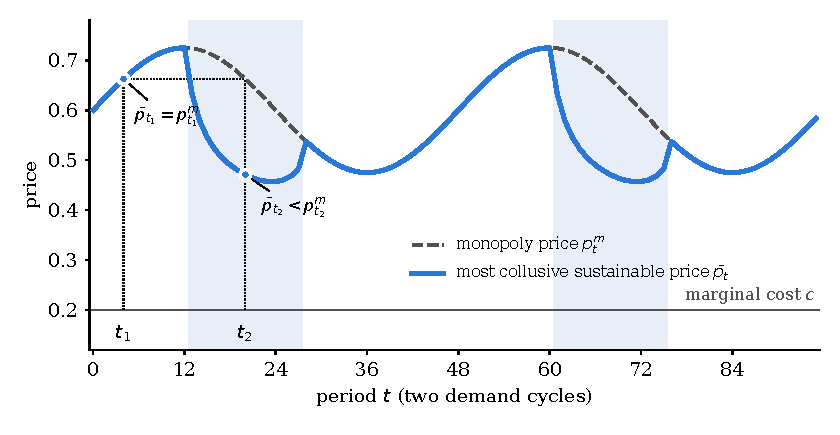
\includegraphics[width=0.92\textwidth]{figures/ch13/bs_cycle.pdf}
\caption{Most collusive sustainable price over a deterministic demand cycle. Linear demand
$D_t(p)=a_t-p$ with $a_t=1+0.25\sin\left(\frac{2\pi t}{48}\right)$, marginal cost $c=0.2$, $N=8$ firms,
$\delta=0.99$ per period and a ten-period Bertrand punishment. Shaded periods are those in which the
incentive constraint \eqref{eq:13-gas-ic} binds. Demand is the same at $t_1$ (rising) and $t_2$ (falling),
yet $\bar p_{t_1}=p^m_{t_1}=0.66$ while $\bar p_{t_2}=0.47$. The path solves \eqref{eq:13-gas-fixed} by
iteration (script \texttt{bs\_cycle.py}).}
\label{fig:13-bs-cycle}
\end{figure}

\casehead{From the incentive constraint to a margin regression}
To motivate an estimating equation we linearize the binding constraint. Let $M_t=\bar p_t-c_t$ be the
collusive margin, $L_t=\frac{M_t}{\bar p_t}$ the Lerner index (a local use of $L_t$, which denotes the lakes
dummy in \cref{sec:13-jec}), and
$\varepsilon_t=-\frac{d'(\bar p_t)\bar p_t}{d(\bar p_t)}$ the industry demand elasticity. At a binding date,
taking logs of $(N-1)A_tM_td(c_t+M_t)=\Phi_t$ gives
\begin{equation*}
\ln A_t+\ln M_t+\ln d(c_t+M_t)=\ln\Phi_t-\ln(N-1).
\end{equation*}
Differentiate, using $\frac{d'}{d}=-\frac{\varepsilon_t}{\bar p_t}$:
\begin{equation*}
\Big(\frac{1}{M_t}-\frac{\varepsilon_t}{\bar p_t}\Big)\,\dd M_t=\dd\ln\Phi_t-\dd\ln A_t+\frac{\varepsilon_t}{\bar p_t}\,\dd c_t .
\end{equation*}
The bracket equals $\frac{1-\varepsilon_tL_t}{M_t}$. It is positive below the monopoly price, because there
profit rises with price: $\frac{\dd}{\dd p}\big[(p-c_t)d(p)\big]=d(p)\,(1-\varepsilon_tL_t)>0$. Near a stationary
point the weights
$\omega_s=\frac{\delta^s}{\sum_{r=1}^{T}\delta^r}$ give $\dd\ln\Phi_t=\sum_s\omega_s\,\dd\ln\bar v_{t+s}$. Hold
future margins at their stationary values, so that future profits move only through demand and cost:
$\dd\ln\bar v_{t+s}=\dd\ln A_{t+s}-\frac{\varepsilon}{\bar p}\dd c_{t+s}$. Substituting and collecting terms,
\begin{equation}\label{eq:13-gas-linear}
\dd M_t=\frac{M}{1-\varepsilon L}\sum_{s=1}^{T}\omega_s\big(\dd\ln A_{t+s}-\dd\ln A_t\big)
-\frac{\varepsilon L}{1-\varepsilon L}\sum_{s=1}^{T}\omega_s\big(\dd c_{t+s}-\dd c_t\big).
\end{equation}
The current levels of demand and cost enter only through their expected changes. With a one-period horizon
and expectations formed at $t$, the margin equation becomes
\begin{equation}\label{eq:13-gas-reg}
M_t\approx\alpha_0+\alpha_2\,\E_t\big[\Delta\ln A_{t+1}\big]+\alpha_3\,\E_t\big[\Delta c_{t+1}\big],\qquad
\alpha_2=\frac{M}{1-\varepsilon L}>0,\quad \alpha_3=-\frac{\varepsilon L}{1-\varepsilon L}<0 .
\end{equation}
The coefficients $\alpha_2$ and $\alpha_3$ are local to this section and have nothing to do with the logit
price coefficient. Under the static benchmark of \cref{prop:13-gas-cs}(c), $\alpha_2=\alpha_3=0$. This is
the null hypothesis that \citet{BorensteinShepard1996} test.

If punishments last longer than one period, the one-period expected change is only a proxy for the weighted
change in \eqref{eq:13-gas-linear}. Under the static null the margin responds to neither, so the proxy
coefficients are still zero and the test keeps its size. Under the alternative the direction of the bias is not
determined. Take demand, and let $\Delta^{1}_t = \E_t[\Delta\ln A_{t+1}]$ and
$\Delta^{T}_t = \sum_{s=1}^{T}\omega_s\E_t[\ln A_{t+s} - \ln A_t]$, both residualized on the other regressors.
Since the weights sum to one, $\Delta^{T}_t = \Delta^{1}_t + R_t$, with $R_t$ the residual of
$\sum_{s=2}^{T}\omega_s\E_t[\ln A_{t+s} - \ln A_{t+1}]$ on the other regressors. Ignoring the cross effect through the cost proxy, the
coefficient on $\Delta^{1}_t$ converges to
\begin{equation*}
\alpha_2\,\frac{\Cov(\Delta^{1}_t, \Delta^{T}_t)}{\Var(\Delta^{1}_t)}
= \alpha_2\left[1 + \frac{\Cov(\Delta^{1}_t, R_t)}{\Var(\Delta^{1}_t)}\right] .
\end{equation*}
The estimate is attenuated only if later expected changes are negatively correlated with the next one, and not so
strongly that the sign reverses. On a smooth seasonal cycle with a horizon of a few months, expected changes in
consecutive months tend to share a sign. The ratio then exceeds one, and the estimate overstates $\alpha_2$. The
same argument applies to $\alpha_3$.

\begin{remark}[Why level and change can be separated]\label{rem:13-gas-level-change}
With independent draws, $\E_t[\ln A_{t+1}]$ is a constant, so $\E_t[\Delta\ln A_{t+1}]=\text{const}-\ln A_t$.
The level of demand and its expected change are then perfectly collinear, and a high level always signals
an expected fall. A seasonal cycle breaks the collinearity. Two weeks with the same demand, one before and
one after the seasonal peak, have opposite expected changes. That is why the test needs predictable
movements in demand and cost.
\end{remark}

\casehead{Competing explanations and the sign of the cost effect}
Two non-collusive mechanisms could also tie current margins to expected future conditions. Both predict
the opposite sign for the cost effect. The first is inventories. Suppose a supplier prices off its
replacement cost, the terminal price $w_{t+1}$ expected at its next purchase, and adds a constant margin
$m^{\circ}$. Then $p_t=\E_t[w_{t+1}]+m^{\circ}$, and the observed margin is
\begin{equation}\label{eq:13-gas-inventory}
M_t=p_t-w_t=m^{\circ}+\E_t\big[\Delta w_{t+1}\big].
\end{equation}
The coefficient on the expected cost change is $+1$, while collusion predicts $\alpha_3<0$. The second
mechanism is a cost of changing prices. A firm facing such costs moves its price toward the price it expects
to want in the future. An anticipated cost increase then raises today's price and today's margin, again a
positive sign. A negative coefficient on expected cost changes is therefore a distinctive prediction of
dynamic collusion. Inventory motives tied to demand require a risk of stockouts, which
\citet{BorensteinShepard1996} rule out because wholesale purchases were never constrained in their sample.

\subsection{Margins and expected demand in U.S.\ cities: Borenstein and Shepard (1996)}\label{sec:13-bs}

\casehead{Question}
Earlier tests of collusion used contemporaneous prices, quantities and costs, as in the conduct-parameter
studies of \cref{ch:conduct}. \citet{Bresnahan1989} stressed that such tests rest on functional-form
assumptions, because static non-cooperative prices can move either way with demand. \citet{BorensteinShepard1996}
ask whether current retail gasoline margins respond to \emph{expected} changes in demand and wholesale cost.
Under static pricing they should not respond at all, so a response is evidence of dynamic collusion that
does not depend on the shape of demand or cost. The question matters because gasoline retailing is far from
a tight oligopoly. Most metropolitan areas have more than ten wholesale suppliers and many more stations.

\casehead{Setting}
Crude oil is refined and shipped by pipeline or barge to city terminals. From the terminal, gasoline is
trucked to stations either by independent wholesalers, called \emph{jobbers}, or by refiners. Jobbers
distribute about 55 percent of U.S. retail gasoline and pay the posted terminal price
(working paper, pp.~8--10). Refiners sell to independently operated stations at the \emph{dealer tankwagon}
price, which is subject to widespread unobserved discounts. Borenstein and Shepard therefore measure
marginal cost by the terminal price. It is the only observed wholesale price for jobbers, it is the
opportunity cost of gasoline sold at refiner-supplied stations, and it is rarely discounted. The margin they
study is the gap between the retail price and the terminal price. It mixes decisions of refiners, jobbers and
station operators.

\casehead{Data}
The panel covers 59 cities in 43 states over the 72 months from 1986 to 1991. \textit{RETAIL} is the Lundberg
Survey average price of regular unleaded self-service gasoline, net of all taxes, on one Friday each month.
\textit{TERM} is the average branded terminal price posted on the same Friday, so the two prices match exactly
and $\textit{MARGIN}=\textit{RETAIL}-\textit{TERM}$. Volume comes from monthly state sales reported by the
Federal Highway Administration. Daily volume in adjacent months is interpolated linearly to the survey day,
giving \textit{VOLUME}. Because over 99 percent of the variance of \textit{VOLUME} is between states,
volume is normalized by its state mean: $\textit{NVOLUME}_{it}=\frac{\textit{VOLUME}_{it}}{\overline{\textit{VOLUME}}_i}$.
\Cref{tab:13-bs-t1} reports the summary statistics. Demand peaks in August at about 20 percent above the
January trough. Short-run demand elasticities lie between $-0.1$ and $-0.2$ \citep{DahlSterner1991}. Retail
prices would then have to swing by 100--200 percent to generate such a cycle, so the seasonal pattern reflects
shifts of demand rather than movements along it. Over half of the monthly crude oil price changes exceed 5
percent in absolute value.

\begin{table}[htbp]
\centering
\caption{Retail gasoline in 59 U.S. cities, 1986--1991: summary statistics}\label{tab:13-bs-t1}
\begin{tabular}{lrrrr}
\toprule
Variable & Mean & Std.\ dev. & Min & Max\\
\midrule
\textit{RETAIL} (cents per gallon) & 72.83 & 12.41 & 43.18 & 126.57\\
\textit{TERM} (cents per gallon) & 62.28 & 11.82 & 36.00 & 111.88\\
\textit{CRUDE} (cents per gallon) & 46.38 & 10.77 & 25.83 & 87.98\\
\textit{MARGIN} (cents per gallon) & 10.57 & 5.12 & $-8.91$ & 34.90\\
\textit{VOLUME} ($10^5$ or $10^6$ gallons per day, see notes) & 10.43 & 10.48 & 0.38 & 38.12\\
\textit{NVOLUME} & 1.005 & 0.087 & 0.570 & 1.617\\
\textit{EXP VOLCHG}, $\hat\eta=-0.1$ & 0.000 & 0.050 & $-0.403$ & 0.287\\
\textit{EXP TERMCHG} (cents per gallon) & 0.139 & 4.172 & $-17.313$ & 13.959\\
\bottomrule
\end{tabular}

\smallskip
\begin{minipage}{0.86\textwidth}\footnotesize
Notes: 3,838 city-month observations. Prices exclude sales and excise taxes and are in current cents.
\textit{EXP VOLCHG} and \textit{EXP TERMCHG} are the expected one-month changes in normalized volume and in the
terminal price defined in the text. The unit of \textit{VOLUME} is unclear in the sources. The working paper's Table 1
prints it as ``(00,000 gal/day)'' and the published Table 1 as gallons $\times 10^{5}$ per day (p.~434). The volume figures
of both versions label the same daily state series in millions of gallons, at levels close to the table means (published
Figure 2, p.~437). We report the numbers as printed and leave the unit open. \textit{NVOLUME} and the regressions do not
depend on it. Source: \citet{BorensteinShepard1996}, working-paper version, Table 1.
\end{minipage}
\end{table}

\casehead{The estimating equation}
Retail prices adjust to terminal prices with lags, and increases pass through faster than decreases. The
authors start from an error-correction model with asymmetric adjustment (working paper, eq.~(1)):
\begin{equation}\label{eq:13-bs-ecm}
\begin{aligned}
\textit{RETAIL}_{it}-\textit{RETAIL}_{i,t-1}={}&\beta_1\Delta\textit{TERM}^{+}_{it}+\beta_2\Delta\textit{TERM}^{+}_{i,t-1}+\beta_3\Delta\textit{TERM}^{+}_{i,t-2}\\
&+\beta_4\Delta\textit{TERM}^{-}_{it}+\beta_5\Delta\textit{TERM}^{-}_{i,t-1}+\beta_6\Delta\textit{TERM}^{-}_{i,t-2}\\
&+\beta_7\Delta\textit{RETAIL}^{+}_{i,t-1}+\beta_8\Delta\textit{RETAIL}^{+}_{i,t-2}\\
&+\beta_9\Delta\textit{RETAIL}^{-}_{i,t-1}+\beta_{10}\Delta\textit{RETAIL}^{-}_{i,t-2}\\
&+\beta_{11}\textit{RETAIL}_{i,t-1}+\beta_{12}\textit{TERM}_{i,t-1}+e_{it}.
\end{aligned}
\end{equation}
Here $\Delta X_{it}=X_{it}-X_{i,t-1}$, and $\Delta X^{+}$ and $\Delta X^{-}$ are the positive and negative parts
of the change. The lagged levels form the error-correction term. If the long-run relation is
$\textit{RETAIL}=\gamma_0+\gamma_1\textit{TERM}$ and the gap closes at rate $\kappa>0$, the correction
$-\kappa(\textit{RETAIL}_{t-1}-\gamma_0-\gamma_1\textit{TERM}_{t-1})$ produces the two lagged levels, with
$\beta_{11}=-\kappa$ and $\beta_{12}=\kappa\gamma_1$. The constant is absorbed by fixed effects.

To put the margin on the left, add $\textit{RETAIL}_{i,t-1}$ to both sides and subtract $\textit{TERM}_{it}$.
The left side becomes $\textit{MARGIN}_{it}$. On the right, $\textit{TERM}_{it}=\Delta\textit{TERM}^{+}_{it}+
\Delta\textit{TERM}^{-}_{it}+\textit{TERM}_{i,t-1}$, so subtracting it lowers the coefficients on
$\Delta\textit{TERM}^{+}_{it}$ and $\Delta\textit{TERM}^{-}_{it}$ by one and the coefficient on
$\textit{TERM}_{i,t-1}$ by one. Adding $\textit{RETAIL}_{i,t-1}$ raises its coefficient by one. The margin
form (working paper, eq.~(2)) is therefore \eqref{eq:13-bs-ecm} with $\beta_1-1$, $\beta_4-1$, $\beta_{11}+1$
and $\beta_{12}-1$ in place of $\beta_1$, $\beta_4$, $\beta_{11}$ and $\beta_{12}$. Adding current volume and the
two expectation terms gives the estimating equation (working paper, eq.~(3)), in which the coefficient
adjustments are left implicit:
\begin{equation}\label{eq:13-bs-main}
\begin{aligned}
\textit{MARGIN}_{it}={}&\alpha_1\textit{NVOLUME}_{it}+\alpha_2\textit{EXP VOLCHG}_{it}+\alpha_3\textit{EXP TERMCHG}_{it}\\
&+\sum_{k=0}^{2}\big(\beta^{+}_{k}\Delta\textit{TERM}^{+}_{i,t-k}+\beta^{-}_{k}\Delta\textit{TERM}^{-}_{i,t-k}\big)\\
&+\sum_{k=1}^{2}\big(\phi^{+}_{k}\Delta\textit{RETAIL}^{+}_{i,t-k}+\phi^{-}_{k}\Delta\textit{RETAIL}^{-}_{i,t-k}\big)\\
&+\beta_{11}\textit{RETAIL}_{i,t-1}+\beta_{12}\textit{TERM}_{i,t-1}+\mu_i+\lambda_t+e_{it}.
\end{aligned}
\end{equation}
We have relabeled the twelve $\beta$'s of the original to show the pattern. The terms $\mu_i$ and
$\lambda_t$ (local symbols here) are city fixed effects and 72 month fixed effects, which absorb cross-city correlation of the
errors at a point in time. Current volume $\alpha_1$ captures any static effect of demand on margins, such as
changes in the mix of customers or peak-load pricing. The coefficients of interest are $\alpha_2$ and
$\alpha_3$, the empirical counterparts of \eqref{eq:13-gas-reg}. The effect of current volume holding expected
next-month volume fixed is $\alpha_1-\alpha_2$, because $\textit{EXP VOLCHG}$ is expected next-month volume
minus current volume.

\casehead{Endogeneity of volume: an instrument built from an assumed elasticity}
Volume depends on the retail price and hence on the margin, so OLS is inconsistent, and no excluded demand
shifters are available. The authors resolve the problem with a constructed instrument. Write the system
(working paper, eqs.~(4) and~(5))
\begin{equation}\label{eq:13-bs-system}
M=a\,Q+X^{\top}g+e,\qquad \ln Q=Z\beta+\eta\ln P+v.
\end{equation}
Here $M$ is the margin, $Q$ volume, $P$ the retail price and $X$ the exogenous variables in the margin
equation. $Z$ collects demand shifters, $\eta<0$ is the industry demand elasticity, and $e$ and $v$ are errors.
The working paper assumes only that $e$ and $v$ are uncorrelated. We assume instead that the margin error is mean
independent of the exogenous variables and of the demand shock, $\E[e\mid X,Z,v]=0$. If $\eta$ were known, the
variable
\begin{equation}\label{eq:13-bs-qprime}
\ln Q'=\ln Q+\ln k-\eta\ln P=Z\beta+\ln k+v
\end{equation}
would be volume purged of the direct price effect. It is a function of $Z$ and $v$ only. Mean independence
therefore makes it, and any function of it, uncorrelated with $e$. It is correlated with $Q$, so it is a valid
instrument. The stronger condition matters because the instrument used below is the level $Q'$, which is
proportional to $\exp(v)$ given $Z$. Uncorrelatedness does not carry over to the level. If $v$ is uniform on
$\{-1,0,1\}$ and $e=v^2-\frac{2}{3}$, then $\E[e]=\E[ev]=0$ but
$\E[e\exp(v)]=\frac{\exp(1)+\exp(-1)-2}{9}>0$. Some demand shifters may themselves respond to
$P$, for example prices of other goods that rise with transport costs. Partition $Z=(Z_1,Z_2)$ with
$Z_1=\theta_0+\theta_1\ln P$ and $Z_2$ independent of $P$. Then
\begin{equation*}
\ln Q=(\theta_0+\theta_1\ln P)\beta_1+Z_2\beta_2+\eta\ln P+v,
\end{equation*}
and the variable
\begin{equation}\label{eq:13-bs-qdoubleprime}
\ln Q''=\ln Q+\ln k-\tilde\eta\ln P=\theta_0\beta_1+Z_2\beta_2+\ln k+v,\qquad \tilde\eta\equiv\eta+\theta_1\beta_1,
\end{equation}
is again a valid instrument if $\E[e\mid X,Z_2,v]=0$. Published estimates of gasoline demand elasticities ignore such indirect effects,
so they are best read as estimates of $\tilde\eta$.

The implementation multiplies daily volume by $kP^{-\hat\eta}$ with $k=\frac{\bar P^{\hat\eta}}{\bar Q}$,
where $\bar P$ is the city's mean retail price and $\bar Q$ the mean of the corrected series. The result,
$\textit{TNVOLUME}=\frac{\textit{VOLUME}}{\bar Q}\left(\frac{P}{\bar P}\right)^{-\hat\eta}$, instruments
\textit{NVOLUME} in two-stage least squares. Since $\hat\eta$ is unknown, the regression is repeated for
$\hat\eta\in\{0,-0.1,-0.2,-0.3\}$, a range slightly wider than the $-0.1$ to $-0.2$ found with monthly and
quarterly data. With $\hat\eta=0$ the correction is void and \textit{NVOLUME} is treated as exogenous. The
correction is small: a price 20 percent above the city mean raises \textit{TNVOLUME} relative to
\textit{NVOLUME} by $1.2^{0.3}-1=5.6$ percent when $\hat\eta=-0.3$ and by $1.2^{0.1}-1=1.8$ percent when
$\hat\eta=-0.1$.

The contemporaneous terminal price could also be endogenous if the marginal cost of supplying a city rises
with its volume. The authors argue that the feedback is small, because terminals have ten or more refiners
and supply can shift across regions. A Hausman test nonetheless rejects exogeneity of the current terminal
price and of the expected terminal-price change. The current price is therefore instrumented with the residual
from a regression of \textit{TERM} on \textit{NVOLUME}. The expected change is instrumented with a forecast built
from that orthogonalized series. Instrumenting does not change the results in an economically or statistically
meaningful way. The residuals of \eqref{eq:13-bs-main}
are not serially correlated, so the lagged dependent variables raise no endogeneity problem.

\casehead{Measuring expectations}
Expected volume comes from a forecasting regression estimated state by state (working paper, eq.~(8)):
\begin{equation}\label{eq:13-bs-volforecast}
\textit{NVOLUME}_{it}=a_0+a_1\textit{NVOLUME}_{i,t-1}+a_2\textit{NVOLUME}_{i,t-2}+\sum_{j=2}^{12}\varsigma_j\textit{MONTH}_j
+a_3t+a_4t^2+a_5t^3+e_{it}.
\end{equation}
The $R^2$ lies between 0.80 and 0.95 for nearly all states. The one-period lead of the fitted values gives
$\textit{EXP VOLCHG}_{it}=\widehat{\textit{NVOLUME}}_{i,t+1}-\textit{NVOLUME}_{it}$. The instrument for
\textit{EXP VOLCHG} uses the same regression estimated with \textit{TNVOLUME}. Expected terminal prices come
from a city-level error-correction autoregression with crude oil prices (working paper, eq.~(9)):
\begin{equation}\label{eq:13-bs-termforecast}
\begin{aligned}
\Delta\textit{TERM}_{it}={}&b_0+\sum_{k=1}^{2}\big(b^{+}_k\Delta\textit{TERM}^{+}_{i,t-k}+b^{-}_k\Delta\textit{TERM}^{-}_{i,t-k}
+d^{+}_k\Delta\textit{CRUDE}^{+}_{i,t-k}+d^{-}_k\Delta\textit{CRUDE}^{-}_{i,t-k}\big)\\
&+b_9\textit{TERM}_{i,t-1}+b_{10}\textit{CRUDE}_{i,t-1}+\sum_{j=2}^{12}\varsigma'_j\textit{MONTH}_j+e_{it}.
\end{aligned}
\end{equation}
The current crude price is excluded because it would not be known when the forecast is made. The $R^2$ ranges
from 0.30 to 0.60, lower than for volume because crude prices behave roughly like a random walk. Then
$\textit{EXP TERMCHG}_{it}=\widehat{\Delta\textit{TERM}}_{i,t+1}$. The forecasting coefficients use the whole
sample, which in principle includes information the firms did not have. Forecasts from rolling regressions
with volume data back to 1982 change neither the predictions nor the final coefficients substantively.

\casehead{Identification}
The month fixed effects absorb any national seasonal pattern, including the common August peak. The
coefficient on \textit{EXP VOLCHG} is therefore identified from differences in seasonal patterns across states
and from state-specific trends. These differences are large. The peak-to-trough swing is 51 percent of mean
volume in Wyoming and 7 percent in Arizona. August demand is below the state mean in Florida, and January
demand is above it in Colorado and Hawaii (working paper, p.~27). The coefficient on \textit{EXP TERMCHG} is
identified from city-specific terminal-price dynamics. Cold-weather cities, for instance, see winter declines
in gasoline terminal prices when refiners produce heating oil and gasoline jointly. The expectation terms are
functions of lagged variables and deterministic seasonals, so they are predetermined with respect to the
current margin shock.

\casehead{Results}
\Cref{tab:13-bs-t2} reproduces the two-stage least squares estimates. The coefficient on \textit{EXP VOLCHG} is
positive and significant at the 1 percent level for every assumed elasticity, and it changes little with
$\hat\eta$. The coefficient on \textit{EXP TERMCHG} is negative and significant at the 1 percent level
throughout. Both signs are those of \eqref{eq:13-gas-reg}. The negative cost coefficient is the opposite of the
inventory prediction \eqref{eq:13-gas-inventory}.

\begin{table}[htbp]
\centering
\caption{Retail margins and expected changes in demand and cost (dependent variable \textit{MARGIN})}\label{tab:13-bs-t2}
\small
\begin{tabular}{lcccc}
\toprule
Assumed elasticity & $\hat\eta=0$ & $\hat\eta=-0.1$ & $\hat\eta=-0.2$ & $\hat\eta=-0.3$\\
\midrule
$\textit{NVOLUME}_t$ & 3.397 (0.754) & 5.563 (0.758) & 7.926 (0.768) & 10.455 (0.785)\\
$\textit{EXP VOLCHG}_t$ & 4.081 (1.324) & 3.860 (1.335) & 4.362 (1.365) & 5.492 (1.409)\\
$\textit{EXP TERMCHG}_t$ & $-0.057$ (0.018) & $-0.062$ (0.017) & $-0.066$ (0.018) & $-0.068$ (0.018)\\
\addlinespace
$\Delta\textit{TERM}^{+}_t$ & $-0.303$ (0.021) & $-0.305$ (0.021) & $-0.306$ (0.021) & $-0.304$ (0.021)\\
$\Delta\textit{TERM}^{+}_{t-1}$ & 0.153 (0.023) & 0.148 (0.023) & 0.143 (0.023) & 0.138 (0.023)\\
$\Delta\textit{TERM}^{+}_{t-2}$ & 0.065 (0.021) & 0.063 (0.021) & 0.062 (0.021) & 0.061 (0.022)\\
$\Delta\textit{TERM}^{-}_t$ & $-0.589$ (0.019) & $-0.584$ (0.019) & $-0.578$ (0.019) & $-0.572$ (0.018)\\
$\Delta\textit{TERM}^{-}_{t-1}$ & 0.175 (0.023) & 0.169 (0.023) & 0.163 (0.023) & 0.155 (0.023)\\
$\Delta\textit{TERM}^{-}_{t-2}$ & 0.078 (0.020) & 0.074 (0.020) & 0.069 (0.020) & 0.065 (0.020)\\
$\Delta\textit{RETAIL}^{+}_{t-1}$ & $-0.017$ (0.022) & $-0.018$ (0.023) & $-0.020$ (0.023) & $-0.022$ (0.023)\\
$\Delta\textit{RETAIL}^{+}_{t-2}$ & $-0.066$ (0.022) & $-0.069$ (0.022) & $-0.072$ (0.022) & $-0.076$ (0.022)\\
$\Delta\textit{RETAIL}^{-}_{t-1}$ & $-0.029$ (0.022) & $-0.027$ (0.022) & $-0.026$ (0.023) & $-0.025$ (0.023)\\
$\Delta\textit{RETAIL}^{-}_{t-2}$ & 0.039 (0.020) & 0.039 (0.020) & 0.039 (0.020) & 0.039 (0.020)\\
$\textit{RETAIL}_{t-1}$ & 0.623 (0.015) & 0.619 (0.015) & 0.615 (0.015) & 0.612 (0.015)\\
$\textit{TERM}_{t-1}$ & $-0.668$ (0.020) & $-0.660$ (0.020) & $-0.650$ (0.020) & $-0.639$ (0.020)\\
\addlinespace
Observations & 3,838 & 3,838 & 3,838 & 3,838\\
\bottomrule
\end{tabular}

\smallskip
\begin{minipage}{0.92\textwidth}\footnotesize
Notes: Two-stage least squares estimates of \eqref{eq:13-bs-main} with city and month fixed effects (not
reported). Asymptotic standard errors in parentheses. \textit{NVOLUME} is instrumented with the
elasticity-corrected series for the assumed $\hat\eta$. Source: \citet{BorensteinShepard1996}, working-paper
version, Table 2.
\end{minipage}
\end{table}

\begin{example}[Reading the magnitudes]\label{ex:13-bs-elasticity}
Take the column $\hat\eta=-0.1$, which the authors regard as closest to the true elasticity. Raise expected
next-month volume by 1 percent of its mean, that is by $0.01005$ units of \textit{NVOLUME}, holding current
volume fixed. \textit{EXP VOLCHG} rises by the same amount, so the margin rises by $3.860\times0.01005=0.039$
cents, which is $\frac{0.039}{10.57}=0.37$ percent of the mean margin. The elasticity of the margin with respect
to expected next-month volume is therefore 0.37. Raise the expected next-month terminal price by 1 percent of its
mean, or 0.623 cents. The margin falls by $0.062\times0.623=0.039$ cents, an elasticity of $-0.37$. These are the
two elasticities in the authors' abstract. A one-standard-deviation increase in \textit{EXP VOLCHG} (0.050) adds
$3.860\times0.050=0.19$ cents to the margin. A one-standard-deviation increase in \textit{EXP TERMCHG} (4.172
cents) subtracts $0.062\times4.172=0.26$ cents.

The seasonal peak shows how the two volume terms combine. July volume averages 8.3 percent above the sample
mean, which adds $5.563\times0.083=0.46$ cents to the July margin. August volume is 8.8 percent above the mean,
so the expected July-to-August change of 0.5 percent adds $3.860\times0.005=0.02$ cents, for a total of 0.48 cents.
In August, current volume adds $5.563\times0.088=0.49$ cents. The expected fall of 4.6 percent into September
subtracts $3.860\times0.046=0.18$ cents, so August margins are only 0.31 cents above average. Margins are higher
on the way up to the peak than at the peak itself, as \cref{fig:13-bs-cycle} predicts.
\end{example}

The rest of the table describes price adjustment. A one-cent rise in the terminal price lowers the margin in
the same month by 0.305 cents, so the retail price rises by $1-0.305=0.70$ cents within the month. A one-cent
fall raises the margin by 0.584 cents, so the retail price falls by only $1-0.584=0.42$ cents. Increases pass
through faster than decreases. The long-run pass-through follows from the lagged levels. Setting all changes to
zero in \eqref{eq:13-bs-main} gives $\textit{RETAIL}(1-\beta_{11})=\textit{TERM}(1+\beta_{12})+\text{const}$, so
\begin{equation*}
\frac{\partial\,\textit{RETAIL}}{\partial\,\textit{TERM}}\bigg|_{\text{long run}}=\frac{1+\beta_{12}}{1-\beta_{11}}
=\frac{1-0.660}{1-0.619}=0.89 .
\end{equation*}
This matches the authors' statement that terminal price changes are passed through about 90 percent in the long
run, a rate they cannot distinguish statistically from 100 percent.

\begin{example}[How large should the effects be?]\label{ex:13-gas-calibration}
The linearized constraint \eqref{eq:13-gas-reg} gives a benchmark for the coefficients. Take the sample means
$M=10.57$ and $\bar p=72.83$ cents, so $L=0.145$, and an industry elasticity between 0.1 and 0.3. Then
$\varepsilon L$ lies between 0.015 and 0.044. The benchmark is $\alpha_2=\frac{M}{1-\varepsilon L}$, between 10.7
and 11.1 cents per unit change in $\ln A$, and $\alpha_3=-\frac{\varepsilon L}{1-\varepsilon L}$, between $-0.015$
and $-0.045$. The estimates of 3.86 and $-0.062$ are of the same order of magnitude. The comparison is only
indicative. The benchmark assumes that the constraint always binds, that punishments last one month, that the
whole measured margin is collusive and that future margins do not move.
\end{example}

\casehead{Robustness: expected versus unexpected changes}
The main threat is measurement error. Monthly state volumes are matched to a single day's city prices. If
current volume is measured with error and next month's volume contains information about current volume, then
\textit{EXP VOLCHG} could proxy for the true current volume. Since current volume raises margins, this would
mimic the collusive effect. The two explanations differ in their predictions for \emph{unexpected} future
changes. Firms cannot respond to changes they do not foresee, so under collusion unexpected changes have zero
coefficients. Under measurement error, unexpected changes would carry information about current volume as
well. The authors estimate (working paper, eq.~(3$'$))
\begin{equation}\label{eq:13-bs-unx}
\begin{aligned}
\textit{MARGIN}_{it}={}&\alpha_1\textit{EXP VOL}_{it}+\alpha'_1\textit{UNX VOL}_{it}+\alpha_2\textit{EXP VOLCHG}_{it}
+\alpha'_2\textit{UNX VOLCHG}_{it}\\
&+\alpha_3\textit{EXP TERMCHG}_{it}+\alpha'_3\textit{UNX TERMCHG}_{it}\\
&+(\text{price-adjustment terms and fixed effects of \eqref{eq:13-bs-main}})+e_{it}.
\end{aligned}
\end{equation}
Here $\textit{UNX VOLCHG}$ is next month's actual volume change minus its expected value. The terms
$\textit{EXP VOL}$ and $\textit{UNX VOL}$ split current volume into the part predicted a month earlier and the
surprise.
\Cref{tab:13-bs-t3} reports the key rows. Unexpected future volume changes are never significantly positive, and
they differ significantly from expected changes for every nonzero $\hat\eta$. Unexpected terminal changes have
coefficients near zero, significantly different from the expected ones. Unexpected \emph{current} volume
raises margins significantly for every nonzero $\hat\eta$. Margins therefore do respond to current surprises.
Their failure to respond to future surprises is informative.

\begin{table}[htbp]
\centering
\caption{Expected versus unexpected changes (dependent variable \textit{MARGIN})}\label{tab:13-bs-t3}
\small
\begin{tabular}{lcccc}
\toprule
Assumed elasticity & $\hat\eta=0$ & $\hat\eta=-0.1$ & $\hat\eta=-0.2$ & $\hat\eta=-0.3$\\
\midrule
$\textit{EXP NVOLUME}_t$ & 4.116 (0.824) & 5.150 (0.830) & 6.273 (0.846) & 7.478 (0.871)\\
$\textit{UNX NVOLUME}_t$ & 0.926 (1.388) & 7.003 (1.402) & 13.347 (1.447) & 19.751 (1.518)\\
$\textit{EXP VOLCHG}_t$ & 3.720 (1.334) & 4.064 (1.347) & 4.930 (1.382) & 6.129 (1.436)\\
$\textit{UNX VOLCHG}_t$ & 1.178 (1.292) & 0.146 (1.309) & $-1.478$ (1.355) & $-3.532$ (1.425)\\
$\textit{EXP TERMCHG}_t$ & $-0.059$ (0.018) & $-0.059$ (0.018) & $-0.057$ (0.018) & $-0.054$ (0.018)\\
$\textit{UNX TERMCHG}_t$ & 0.013 (0.016) & 0.011 (0.016) & 0.009 (0.016) & 0.006 (0.016)\\
\addlinespace
Observations & 3,838 & 3,838 & 3,838 & 3,838\\
\bottomrule
\end{tabular}

\smallskip
\begin{minipage}{0.92\textwidth}\footnotesize
Notes: Estimates of \eqref{eq:13-bs-unx}. The price-adjustment terms, city and month fixed effects are included
and not shown. Standard errors in parentheses. Source: \citet{BorensteinShepard1996}, working-paper version,
Table 3.
\end{minipage}
\end{table}

\casehead{Interpretation}
Borenstein and Shepard read the evidence as consistent with tacit collusion in the sense of
\citet{RotembergSaloner1986} and \citet{HaltiwangerHarrington1991}. They stress what the test does not show.
Collusion here need not mean prices near monopoly. With an industry elasticity between $-0.1$ and $-0.3$, demand
is inelastic at observed prices, so an industry monopolist would raise prices far above them. The authors conclude
that actual margins fall far short of the monopoly level. Nor does the test measure the level of collusion. The
measured margin includes delivery and other short-run variable costs, so the collusive part is smaller than 10.6
cents, and the data cannot isolate it. What the test detects is the dynamic signature of an incentive constraint.
A mild form of tacit coordination fits the market: a station that cuts
its price provokes nearby stations to retaliate, and the retaliation is costlier when future margins are high.

\casehead{Critiques}
Five limitations deserve mention. First, expectations are the econometrician's forecasts. Their coefficients are
estimated on the full sample, and the true information sets of station managers are unknown. Second, volume is
measured at the state level, prices at the city level, and prices only on one day per month. Third, the
one-month horizon is arbitrary. The authors argue that longer punishments would bias the estimates downward
(working paper, p.~17). That holds only under the covariance condition stated after \eqref{eq:13-gas-reg}, and on
a seasonal cycle the bias can go either way. The test of the static null keeps its size in either case. Fourth, the test rejects static pricing, but other dynamic
non-cooperative models could generate forward-looking prices. \Cref{sec:13-noel} shows that Edgeworth cycles are one
such model, although its mechanism differs from the one tested here. Fifth, the margin mixes the decisions of
refiners, jobbers and station operators, so the colluding agents are not identified.

\casehead{Contribution}
The paper moved the empirical study of collusion from tight oligopolies to an unconcentrated industry with many
differentiated sellers. It replaced contemporaneous price-cost relations, which require functional-form
assumptions, with a dynamic implication of the incentive constraint. It also showed how to build a test that
distinguishes collusion from inventory behavior and from measurement error through sign restrictions and a
placebo on unforecastable changes.

\subsection{Edgeworth cycles in Toronto: Noel (2007)}\label{sec:13-noel}

\casehead{Question}
In many Canadian cities retail gasoline prices follow a fast asymmetric cycle. A large, sudden price increase is
followed by many small decreases until margins are thin, and then prices jump again. Consumer groups and
governments have often read the synchronized jumps as collusion. \citet{Noel2007} asks whether the cycle is
instead a competitive \emph{Edgeworth cycle}, the Markov equilibrium of dynamic price competition introduced by
\citet{MaskinTirole1988}. The answer matters for policy, because evidence of Edgeworth cycles argues against
costly investigations of covert collusion.

\casehead{Theory}
In the model of \citet{MaskinTirole1988}, two firms sell a homogeneous good and set prices alternately, each price
fixed for two periods. Strategies are Markov: the moving firm conditions only on the rival's current price (and,
in the extension of \citet{Noel2007}, on the current cost). With demand $D^i$ for firm $i$ and cost $c_t$, firm
$i$ earns $\pi^i_t(p^1_t,p^2_t,c_t)=D^i(p^1_t,p^2_t)(p^i_t-c_t)$. When firm 1 moves after firm 2 has set
$p^2_{t-1}$, its values are
\begin{align}
V^1(p^2_{t-1})&=\E_c\Big[\max_{p_t}\big\{\pi^1_t(p_t,p^2_{t-1},c_t)+\delta_1W^1(p_t)\big\}\Big],\label{eq:13-mt-v}\\
W^1(p^1_{s-1})&=\E_c\Big[\E_{p_s}\big[\pi^1_s(p^1_{s-1},p_s,c_s)+\delta_1V^1(p_s)\big]\Big].\label{eq:13-mt-w}
\end{align}
Here $W^1$ is firm 1's value in a period in which firm 2 moves, and $p_s$ is firm 2's reply. The game has two
kinds of Markov perfect equilibria, focal-price equilibria and Edgeworth-cycle equilibria. The incentives
behind a cycle are as follows. At a high rival price, undercutting by one step captures the whole market for a
period, roughly twice what matching yields. Prices therefore fall step by step in the \emph{undercutting phase}.
Near marginal cost an undercut earns nothing. Raising the price is costly for the firm that moves first, because
the rival keeps the low price and serves the market for a period. Each firm prefers the other to restore prices,
so the bottom of the cycle is a war of attrition in which firms randomize between staying low and jumping up. The
firm that moves jumps all the way to the top in a single \emph{relenting phase}. A gradual increase would be
undercut at once and would not repay its cost. \Cref{fig:13-edgeworth} draws the resulting sawtooth.

\begin{figure}[htbp]
\centering
\begin{tikzpicture}
\begin{axis}[
  width=0.92\textwidth, height=6.4cm,
  xmin=-0.5, xmax=25, ymin=-0.9, ymax=12.6, clip=false,
  axis lines=left, xtick=\empty, ytick={2}, yticklabels={$c$},
  xlabel={period $t$ (firms move alternately)}, ylabel={price},
  legend style={draw=none, at={(0.5,-0.2)}, anchor=north, font=\footnotesize, legend columns=3,
    /tikz/every even column/.append style={column sep=0.6cm}},
  legend cell align=left,
]
\addplot[const plot, line width=1.6pt, orange!85!black] coordinates {
 (0,2) (1,9) (2,9) (3,7) (4,7) (5,5) (6,5) (7,3) (8,3) (9,2) (10,2) (11,10) (12,10) (13,8)
 (14,8) (15,6) (16,6) (17,4) (18,4) (19,2) (20,2) (21,2) (22,2) (23,9) (24,9) (25,9)};
\addlegendentry{firm 2 (moves at odd $t$)}
\addplot[const plot, line width=0.8pt, blue!70!black] coordinates {
 (0,10) (1,10) (2,8) (3,8) (4,6) (5,6) (6,4) (7,4) (8,2) (9,2) (10,2) (11,2) (12,9) (13,9)
 (14,7) (15,7) (16,5) (17,5) (18,3) (19,3) (20,2) (21,2) (22,10) (23,10) (24,8) (25,8)};
\addlegendentry{firm 1 (moves at even $t$)}
\addplot[dashed, gray, domain=-0.5:25] {2};
\addlegendentry{marginal cost $c$}
\draw[decorate, decoration={brace, amplitude=5pt}] (axis cs:1,10.7) -- (axis cs:9,10.7)
  node[midway, above=6pt, font=\footnotesize] {undercutting phase};
\draw[decorate, decoration={brace, amplitude=5pt, mirror}] (axis cs:8,1.3) -- (axis cs:11,1.3)
  node[midway, below=6pt, font=\footnotesize] {war of attrition};
\draw[-{Stealth[length=2mm]}] (axis cs:13.2,11.6) -- (axis cs:11.2,10.4);
\node[font=\footnotesize, anchor=west] at (axis cs:13.2,11.6) {relenting phase};
\end{axis}
\end{tikzpicture}
\caption{A stylized Edgeworth cycle with two symmetric firms. Each firm's price is fixed for two periods and firms
move in turn. Prices fall by one step per move until they reach marginal cost $c$. After a war of attrition one firm
relents to the top in a single jump, the rival undercuts it at once, and the cycle restarts. Where the two prices
coincide, the thin line lies on the thick one. Drawn by us after the logic of \citet{MaskinTirole1988} and Figure 2
of \citet{Noel2007}.}
\label{fig:13-edgeworth}
\end{figure}

Firm asymmetries sharpen the predictions. \citet{Eckert2003} lets firms split the market unequally at equal
prices. The firm with the smaller share at equal prices gains more from undercutting, since it gives up less of
the shared market, so small firms lead prices down. Large firms, which control many stations and coordinate them
easily, are better placed to restart the cycle. The theory thus makes one structural prediction and three
behavioral ones. The structural prediction is that each station raises its price by the full height of the cycle
in one period and then lowers it in small consecutive steps. The behavioral predictions are (1) fast but not
simultaneous reactions, (2) small firms lead prices down, and (3) large firms lead prices up. Edgeworth cycles
survive cost fluctuations and mild spatial differentiation, so the predictions carry over to retail gasoline.

\casehead{Data}
Noel collected retail prices every twelve hours at 22 Toronto stations on major routes over 131 consecutive days,
February 12 to June 22, 2001. Thirteen stations belong to major integrated firms and nine to independents, twelve
firms in all, spread over 17 miles. The price is for regular unleaded self-service gasoline in Canadian cents per
liter (cpl). The rack price is the daily spot price of the largest wholesaler at the Toronto rack, which can be
treated as exogenous because U.S. wholesale supply is readily available. Excise taxes are 24.7 cpl and the sales
tax is 7 percent. The average price before tax is 43.09 cpl (standard deviation 4.44), and after tax 72.53 (4.75).
The rack price averages 39.77 (4.00). The lagged retail price exceeds the rack price by 3.31 cpl (2.08) on
average (Table I). \Cref{fig:13-noel-f1} shows a major and an independent
station against the rack price. The retail cycle is evident, and the rack price has none.

\begin{figure}[htbp]
\centering
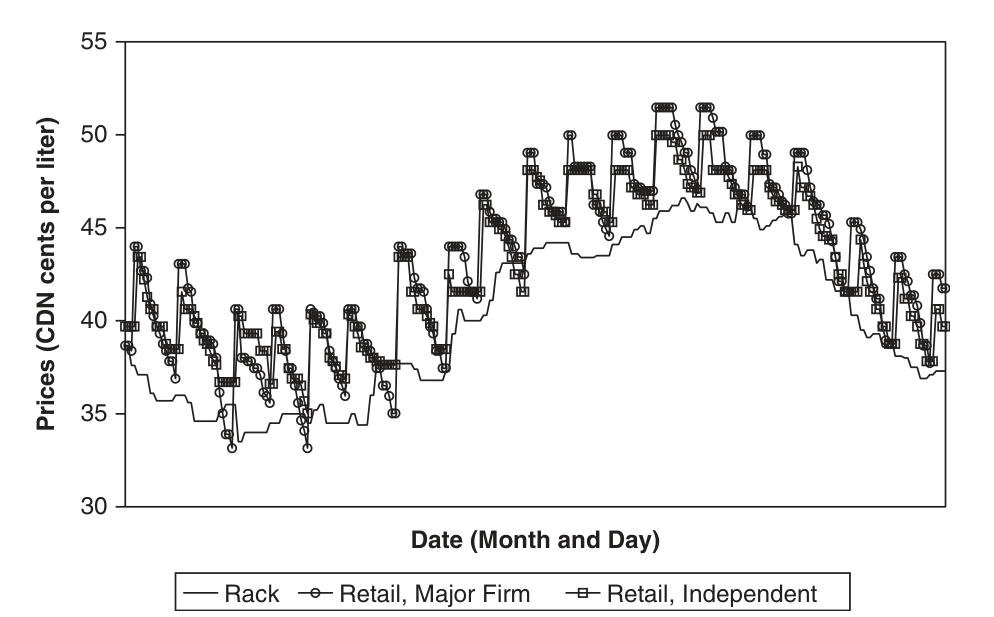
\includegraphics[width=0.78\textwidth]{figures/ch13/noel2007_fig1.png}
\caption{Twelve-hourly retail prices at a major-firm station and an independent station in Toronto, February to
June 2001, with the rack price. Prices exclude taxes. Source: \citet{Noel2007}, Figure 1.}
\label{fig:13-noel-f1}
\end{figure}

\casehead{Model}
For station $s$ in period $t$, the regime $I_{st}\in\{R,U\}$ is either relenting or undercutting. The regime is
latent, because a zero or small change can belong to either phase. Within regime $i$, the price change
$\Delta p_{st}$ follows (Noel's eq.~(4))
\begin{equation}\label{eq:13-noel-regime}
\Delta p_{st}=\begin{cases}X^{i}_{st}\beta^{i}+\epsilon^{i}_{st}, & \text{with probability }1-\gamma^{i}_{st},\\
0, & \text{with probability }\gamma^{i}_{st},\end{cases}\qquad \epsilon^{i}_{st}\sim N(0,\sigma_i^2).
\end{equation}
The mass point at zero allows for stations that skip a period, since the twelve-hour sampling need not match the
true length of a pricing period. The \emph{sticky-price probability} $\gamma^i_{st}$ and the regime transition
probabilities are logits (Noel's eqs.~(5)--(6)):
\begin{equation}\label{eq:13-noel-logits}
\begin{gathered}
\lambda^{iR}_{st}=\Pr\big(I_{st}=R\mid I_{s,t-1}=i,W^i_{st}\big)=\frac{\exp(W^i_{st}\vartheta^i)}{1+\exp(W^i_{st}\vartheta^i)},\qquad
\lambda^{iU}_{st}=1-\lambda^{iR}_{st},\\
\gamma^i_{st}=\frac{\exp(V^i_{st}\zeta^i)}{1+\exp(V^i_{st}\zeta^i)} .
\end{gathered}
\end{equation}
In this subsection $\lambda$ and $\gamma$ are local symbols, and $a_i=\E[\Delta p\mid\Delta p\neq0,\text{regime }i]$
denotes the expected nonzero price change, which Noel writes $\alpha^i$. The density of an observed change in
regime $i$ mixes a point mass and a normal density:
\begin{equation}\label{eq:13-noel-density}
g_i(\Delta p_{st})=\gamma^i_{st}\,\indic\{\Delta p_{st}=0\}+(1-\gamma^i_{st})\,\frac{1}{\sigma_i}\,\phi\Big(\frac{\Delta p_{st}-X^i_{st}\beta^i}{\sigma_i}\Big)\,\indic\{\Delta p_{st}\neq0\},
\end{equation}
where $\phi$ is the standard normal density.
The likelihood is computed with the filter of \cref{sec:13-markov}, following \citet{CosslettLee1985} as in
\citet{Ellison1994}. Let $\xi_{t\mid t-1}(j)$ be the probability of regime $j$ given past price changes. Then
\begin{align*}
\xi_{t\mid t-1}(j)&=\sum_{i\in\{R,U\}}\lambda^{ij}_{st}\,\xi_{t-1\mid t-1}(i),\qquad
f(\Delta p_{st}\mid\text{past})=\sum_{j}\xi_{t\mid t-1}(j)\,g_j(\Delta p_{st}),\\
\xi_{t\mid t}(j)&=\frac{\xi_{t\mid t-1}(j)\,g_j(\Delta p_{st})}{f(\Delta p_{st}\mid\text{past})},\qquad
\ell=\sum_{s}\sum_{t}\ln f(\Delta p_{st}\mid\text{past}).
\end{align*}
The parameters are estimated by maximum likelihood with Newey-West standard errors.

The cycle's characteristics follow from the switching probabilities. With constant probabilities the length of a
spell in regime $i$ is geometric, so its expected duration is $\frac{1}{1-\lambda^{ii}}$ (\cref{lem:13-durations}).
The expected period of the cycle is the sum of the two expected durations. The total price increase during a
relenting spell is the sum of a random number of independent price changes, each with mean $(1-\gamma^R)a_R$.
By Wald's identity its expectation is the product of the mean duration and the mean change:
\begin{equation}\label{eq:13-noel-amplitude}
\E[\text{amplitude}]=\frac{(1-\gamma^R)\,a_R}{1-\lambda^{RR}},\qquad
\E[\text{period}]=\frac{1}{1-\lambda^{RR}}+\frac{1}{1-\lambda^{UU}},\qquad
\text{asymmetry}=\frac{1-\lambda^{RR}}{1-\lambda^{UU}} .
\end{equation}
The asymmetry measure is the ratio of the undercutting duration to the relenting duration. Standard errors come
from the delta method.

\casehead{The anatomy of the cycle}
\Cref{tab:13-noel} reproduces the estimates with constant parameters. The relenting phase lasts 1.008 half-days,
which confirms the structural prediction: each station completes its increase within one twelve-hour period. The
undercutting phase lasts 12.78 half-days, so the cycle repeats about once a week. The amplitude is 5.62 cpl, or 13
percent of the average pre-tax price and 170 percent of the average markup. Increases of 10 cpl in one step were
common in the sample.

\begin{table}[htbp]
\centering
\caption{Regime estimates and cycle characteristics, Toronto 2001}\label{tab:13-noel}
\small
\begin{tabular}{lccc}
\toprule
 & (1) All firms & (2) Major firms & (2) Independents\\
\midrule
\multicolumn{4}{l}{\textit{Relenting phase}}\\
$a_R$ (expected nonzero change, cpl) & 5.576 (0.083) & 5.782 (0.101) & 5.192 (0.142)\\
$\sigma_R$ & 1.650 (0.066) & 1.610 (0.085) & 1.655 (0.100)\\
$\gamma^R$ (sticky share) & 4.0E-5 (4.6E-4) & 4.1E-5 (4.8E-4) & 3.8E-5 (4.9E-4)\\
\multicolumn{4}{l}{\textit{Undercutting phase}}\\
$a_U$ (expected nonzero change, cpl) & $-0.751$ (0.008) & $-0.767$ (0.010) & $-0.720$ (0.015)\\
$\sigma_U$ & 0.459 (0.009) & 0.467 (0.012) & 0.441 (0.012)\\
$\gamma^U$ (sticky share) & 0.429 (0.007) & 0.422 (0.008) & 0.441 (0.014)\\
\multicolumn{4}{l}{\textit{Switching probabilities}}\\
$\lambda^{RR}$ & 0.008 (0.004) & 0.008 (0.005) & 0.007 (0.007)\\
$\lambda^{RU}$ & 0.992 (0.004) & 0.992 (0.005) & 0.993 (0.007)\\
$\lambda^{UR}$ & 0.078 (0.001) & 0.078 (0.002) & 0.078 (0.003)\\
$\lambda^{UU}$ & 0.921 (0.001) & 0.921 (0.002) & 0.921 (0.003)\\
\multicolumn{4}{l}{\textit{Cycle characteristics}}\\
Relenting duration (half-days) & 1.008 (0.004) & 1.008 (0.007) & 1.007 (0.007)\\
Undercutting duration (half-days) & 12.780 (0.291) & 12.779 (0.358) & 12.784 (0.484)\\
Cycle period (half-days) & 13.788 (0.291) & 13.787 (0.358) & 13.792 (0.485)\\
Asymmetry & 12.680 (0.291) & 12.677 (0.363) & 12.687 (0.491)\\
Amplitude (cpl) & 5.619 (0.082) & 5.828 (0.098) & 5.232 (0.144)\\
\bottomrule
\end{tabular}

\smallskip
\begin{minipage}{0.92\textwidth}\footnotesize
Notes: Specification (1) has no firm-type dummies. Specification (2) adds major and independent dummies to $a_i$,
$\lambda^{ij}$ and $\gamma^i$. Standard errors from the delta method in parentheses. Source: \citet{Noel2007},
Tables II and III.
\end{minipage}
\end{table}

\begin{example}[Checking the cycle arithmetic]\label{ex:13-noel-cycle}
From \eqref{eq:13-noel-amplitude}, the relenting duration is $\frac{1}{1-0.008}=1.008$. The undercutting duration of
12.780 implies an unrounded $\lambda^{UU}=1-\frac{1}{12.780}=0.9218$. This rounds to 0.922, one unit in the third
decimal above the 0.921 that the table reports. The period is
$1.008+12.780=13.788$ half-days and the asymmetry is $\frac{12.780}{1.008}=12.68$. The amplitude is
$(1-0.00004)\times5.576\times1.008=5.62$ cpl, equal to the reported 5.619 up to rounding. The descent can be checked
the same way. The expected change per half-day in the undercutting phase is $(1-0.429)\times(-0.751)=-0.43$ cpl, and
over 12.78 half-days prices fall by $0.43\times12.78=5.48$ cpl. Up and down movements nearly balance over a cycle, as
they must when prices show no strong trend over the sample.
\end{example}

\casehead{Small versus large firms}
To test the behavioral predictions, Noel lets the parameters depend on two variables, interacted with firm type.
The first, $\textit{POSITION}_{st}=\textit{RETAIL}_{s,t-1}-\textit{RACK}_{st}-\textit{TAX}_{st}$, measures how far the
station's pre-tax price is above the bottom of the cycle. The second, $\textit{FOLLOW}_{st}$, equals one if some other
station has already relented and station $s$ has not. The probability of switching from undercutting to relenting
rises steeply as margins shrink. For majors it is 0.046 at the mean \textit{POSITION} of 3.31 cpl and 0.110 at 1.53,
the mean just before a relent. It reaches 0.272 at zero and 0.803 at the minimum of $-3.24$ (Table IV). At
$\textit{POSITION}=1.53$ the derivative $\frac{\partial\lambda^{UR}}{\partial\,\textit{POSITION}}$ is $-0.065$ (0.006)
for majors and $-0.051$ (0.006) for independents.

Prediction (2) holds. Near the top of the cycle independents undercut more often and majors keep sticky prices.
Near the bottom the roles reverse. The derivative of the sticky-price probability with respect to \textit{POSITION} is
0.036 (0.002) for majors and $-0.034$ (0.005) for independents (Table V). Large firms try to hold high prices for a
while, then chase the small firms down. Just before a relent majors are often cheaper than independents.

Prediction (3) holds as well, and \cref{tab:13-noel-t5} shows it. When no station has yet relented, a major
relents in a given half-day with probability 0.091 and an independent with probability 0.026. Once some station has
relented, a major follows within half a day with probability 0.925 and an independent with probability 0.720. Both
probabilities are high, which confirms prediction (1): reactions are fast but not simultaneous. With data sampled
every two days or less often, the increases would look perfectly synchronous. A major that follows raises its price
by 0.200 cents less than if it had led, which is the predicted undercut of the leader by the follower. The relenting
jump falls almost one for one with \textit{POSITION} (derivatives $-0.897$ for majors and $-0.873$ for independents),
so stations restore a nearly standard markup.

\begin{table}[htbp]
\centering
\caption{Leaders and followers: probability of switching from undercutting to relenting in a half-day}\label{tab:13-noel-t5}
\small
\begin{tabular}{lcccc}
\toprule
 & \multicolumn{2}{c}{Leaders (no station has relented)} & \multicolumn{2}{c}{Followers (some station has relented)}\\
\cmidrule(lr){2-3}\cmidrule(lr){4-5}
 & Majors & Independents & Majors & Independents\\
\midrule
$\textit{POSITION}=1.53$ & 0.091 (0.006) & 0.026 (0.003) & 0.925 (0.045) & 0.720 (0.045)\\
$\textit{POSITION}=0$ & 0.235 (0.020) & 0.066 (0.011) & 0.974 (0.016) & 0.868 (0.030)\\
\bottomrule
\end{tabular}

\smallskip
\begin{minipage}{0.92\textwidth}\footnotesize
Notes: Entries are $\lambda^{UR}$ from specification (4), in which the relenting jump and the switching probability
depend on firm type, \textit{FOLLOW}, \textit{POSITION} and their interactions. Delta-method standard errors in
parentheses. A \textit{POSITION} of 1.53 cpl is the average just before a relent. Source: \citet{Noel2007}, Table V.
\end{minipage}
\end{table}

\casehead{Competing hypotheses}
Noel rejects four alternatives to Edgeworth cycles. A day-of-the-week demand cycle cannot produce one large jump
followed by daily declines. The jump falls on different weekdays, and periods range from four to ten days. Relents
do cluster early in the week. The first relent of a round comes on Monday 18 percent of the time, Tuesday 32,
Wednesday 22, Thursday 18, Friday 10 and never at weekends. Differences in menu or monitoring costs cannot explain why majors move
faster upward but not downward. Inventory depletion would require station managers to misforecast their sales in the
same direction every period, and deliveries occur on different days for different stations. Rack-price discounts are
below 1 cpl, against an amplitude of 5.6 cpl, and do not vary over time.

The fifth alternative, covert collusion, cannot be excluded by any price pattern, since the folk theorem
(\cref{ch:collusion-theory}) admits many collusive paths. Noel argues that a cycle is an implausible collusive scheme.
Simple rules such as a constant markup are easier to agree on and to monitor. Cycles require fast, differentiated price
moves at hundreds of stations, and their large jumps attract complaints. The data also show no single price leader:
different firms lead the relents, and the ranking of stations changes often during the descent.

\casehead{Interpretation and critiques}
The evidence supports a competitive reading of the Toronto cycle. Its price wars are not punishments: prices fall
repeatedly and predictably as firms compete, and informed consumers can lower what they pay by timing purchases. An
informal poll of 58 residents found that they expected 58 percent of price changes to be increases, whereas 86 percent
of actual changes were decreases. The study has clear limits. It has no quantity data, so it cannot measure welfare or
the station-level elasticity behind the fast undercutting. The sample is 22 stations over 131 days. The tests are
consistency tests, since the theory leaves the amplitude and the top price undetermined. The main caveat for
detection comes from Quebec. \Cref{sec:13-clarkhoude} shows that a documented cartel there also produced asymmetric
cycles. The shape
of the cycle cannot by itself separate competition from collusion. The role assignments of small and large firms carry
more of the evidential weight than the shape. Later work exploits sharper variation, for example a regulation of the
timing of price changes in Perth studied by \citet{Wang2009}.

\subsection{A prosecuted cartel with asymmetric retailers: Clark and Houde (2013)}\label{sec:13-clarkhoude}

\casehead{Question}
Repeated-game theory has long recognized that firms with different costs or sizes need side payments to collude
\citep{JacqueminSlade1989}. Upstream cartels can assign quotas or territories. In a retail market with posted prices,
however, a cartel cannot tell consumers where to shop. At a common price, market shares follow locations and
amenities. They need not match what each firm requires to stay in the cartel. \citet{ClarkHoude2013} ask how a cartel of heterogeneous gasoline
retailers solved this problem, using the record of a prosecuted case.

\casehead{Setting and data}
The cartel came to light after a Victoriaville newspaper published, on June 6, 2004, an interview with station owner
Christian Goulet. He claimed he was harassed for refusing to go along with price fixing. The Canadian Competition
Bureau began recording phone conversations on March 3, 2005 and executed search warrants from May 29, 2006. Charges were
announced on June 12, 2008, with later rounds in 2010 and 2012, against fourteen companies and thirty-nine individuals
in total. By September 2012 seven companies and 27 individuals had pleaded guilty, with company fines from \$90,000 to
\$1,850,000. The case covers 128 stations and 64 firms in Victoriaville, Thetford Mines, Sherbrooke and Magog.

Three sources are combined. The Competition Bureau's court documents summarize or quote the recorded calls for each price
change, with caller, receiver and time. A weekly station-level survey by the Quebec energy board (the R\'egie de
l'\'energie) covers 2002--2005. A quarterly survey by Kent Marketing reports volumes, characteristics and the full
cross-section of prices. The key players differ sharply. Bilodeau (Shell) organized the cartel in Victoriaville and
Thetford Mines and Bourassa (Olco) in Sherbrooke. Both run the largest networks of lessee stations. Ultramar, the only
refiner in eastern Quebec, sets prices centrally and runs a low-price guarantee that commits its stations to post the
lowest price in each neighborhood. Two big-box retailers, Canadian Tire and Maxi, run high-volume stations as loss leaders.
Couche-Tard, the largest convenience-store chain, sets prices through one regional representative.

\casehead{Heterogeneous costs}
Station sizes vary widely. The average Sherbrooke station sells 48.67 thousand liters a week with a standard deviation
of 24.56 (Table 2). Following \citet{Houde2012}, marginal cost is additive in the \emph{minimum estimated price} (MEP), a
weekly price floor published by the R\'egie that stations may not undercut:
\begin{equation}\label{eq:13-ch-mc}
mc_{jt}=\textit{MEP}_t+c_j .
\end{equation}
The station cost differential $c_j$ comes from \citet{Houde2012}. He recovers station marginal costs by inverting the
multi-product Bertrand first-order conditions of a spatial demand model (\cref{ch:diffprod}) and regresses them on station
characteristics. Stations with more pumps, a convenience store or a car wash have lower costs. The differentials range
from $-0.05$ to $-1.98$ cpl in Sherbrooke and from $-0.02$ to $-2.03$ cpl in Victoriaville. Ultramar's stations are on
average 1.6 cpl below the MEP.

\casehead{Price patterns}
Weekly price changes in the cartel cities from 2002 to 2005 form an asymmetric cycle (\cref{fig:13-ch-f1}). Increases are
spread symmetrically around 4 cpl, with an interquartile range of 2 cpl. Cuts cluster at 1 or 2 cpl, and 70 percent are at
most 2 cpl. Floor changes are much more symmetric, so prices rise faster than they fall. Prices were unchanged two weeks in a
row 48 percent of the time in Victoriaville, 57 percent in Thetford Mines and 36 percent in Sherbrooke. The floor was
constant only 1.2 percent of the time. In Victoriaville and Thetford Mines, 95 percent of price changes kept the ending digit
fixed. The cross-section of prices was
concentrated. In Victoriaville the suggested price was 2 cpl above the minimum, and two fringe stations were allowed to post
up to 2 cpl below it. In Thetford Mines self-service stations posted half a cent below full-service ones.

\begin{figure}[htbp]
\centering
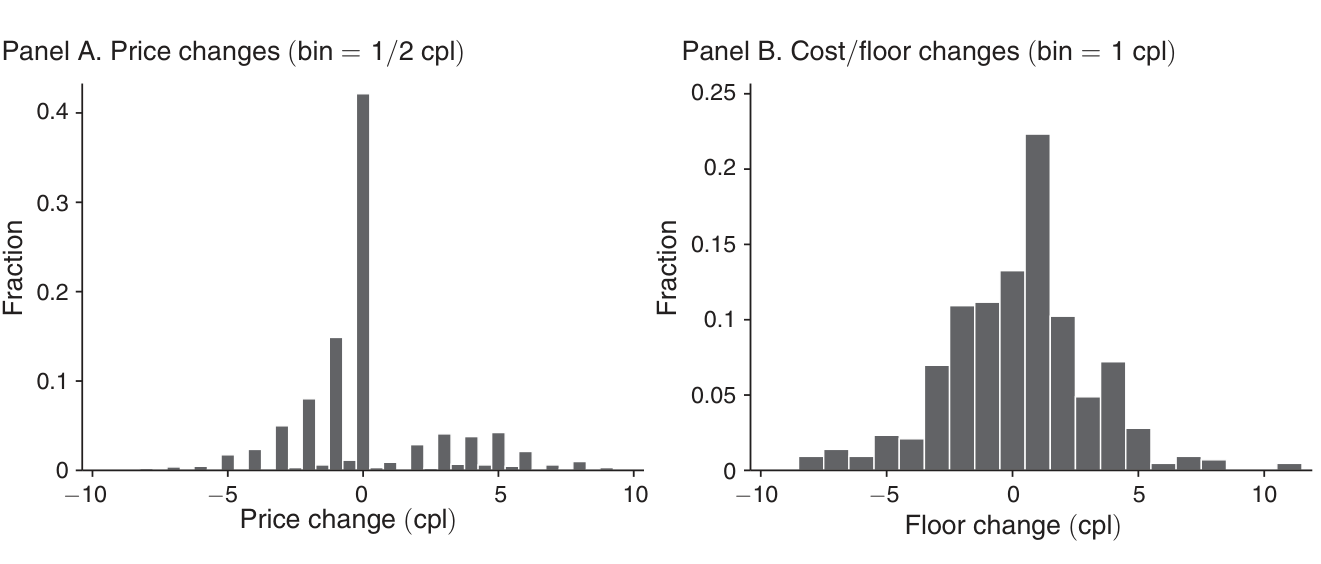
\includegraphics[width=0.88\textwidth]{figures/ch13/clarkhoude2013_fig1.png}
\caption{Distribution of weekly price changes (panel A) and of price-floor changes (panel B) in the cartel cities,
2002--2005. Source: \citet{ClarkHoude2013}, Figure 1.}
\label{fig:13-ch-f1}
\end{figure}

\casehead{Why asymmetry is a problem: a two-firm model}
The authors illustrate the enforcement problem with two retailers of a homogeneous good facing inelastic unit demand.
Firm $H$ has marginal cost $c>0$ and firm $L$ has cost 0. At the cartel price $\bar p$ they hold shares $s_H$ and
$s_L=1-s_H$. After a deviation they play static Bertrand forever, in which $H$ earns zero and $L$ serves the market at price
$c$. The incentive constraints are
\begin{equation}\label{eq:13-ch-ic2}
\textit{IC}^H:\ \frac{s_H(\bar p-c)}{1-\delta}\ge p^d_H-c,\qquad
\textit{IC}^L:\ \frac{s_L\bar p}{1-\delta}\ge p^d_L+\delta\,\frac{c}{1-\delta},
\end{equation}
where $p^d_j$ is the deviation price. The low-cost firm loses less from the punishment, because it keeps the whole market
at price $c$.

\begin{proposition}[Collusion needs an unequal split]\label{prop:13-ch-shares}
In the two-firm model, let deviations undercut $\bar p$ by an arbitrarily small amount. Collusion at $\bar p$ is sustainable
if and only if
\begin{equation*}
\delta\ge\underline\delta(s_L)\equiv\max\Big\{s_L,\ \frac{(1-s_L)\,\bar p}{\bar p-c}\Big\}.
\end{equation*}
The threshold is minimized at $s_L^*=\frac{\bar p}{2\bar p-c}>\frac{1}{2}$, where $\underline\delta(s_L^*)=\frac{\bar p}{2\bar p-c}$.
With equal shares the threshold is $\frac{\bar p}{2(\bar p-c)}$, which is at least one when $c\ge\frac{\bar p}{2}$,
so collusion with equal shares is then impossible for every $\delta<1$.
\end{proposition}

\begin{proof}
Let $p^d_H,p^d_L\to\bar p$. Multiplying $\textit{IC}^H$ by $1-\delta$ gives $s_H(\bar p-c)\ge(1-\delta)(\bar p-c)$, or
$\delta\ge1-s_H=s_L$. Multiplying $\textit{IC}^L$ by $1-\delta$ gives
\begin{equation*}
s_L\bar p\ge(1-\delta)\bar p+\delta c,
\end{equation*}
which rearranges to $\delta(\bar p-c)\ge(1-s_L)\bar p$, or $\delta\ge\frac{(1-s_L)\bar p}{\bar p-c}$. Both must hold, which gives
the maximum. The first term increases in $s_L$ and the second decreases, so the maximum is smallest where they are equal:
$s_L(\bar p-c)=(1-s_L)\bar p$, or $s_L^*=\frac{\bar p}{2\bar p-c}$. Since $c>0$, $s_L^*>\frac{1}{2}$. Substituting $s_L=\frac{1}{2}$
gives $\max\{\frac{1}{2},\frac{\bar p}{2(\bar p-c)}\}=\frac{\bar p}{2(\bar p-c)}$, which is at least one when $\bar p\le2c$.
\end{proof}

The proposition is our formalization of the authors' example. With a large cost gap, collusion on equal shares is
impossible at any discount factor, while a split that favors the low-cost firm sustains it for $\delta$ close to one. The
cartel thus faces an \emph{enforcement problem}, which requires shifting market share toward low-cost and small-network
firms. It also faces a \emph{coordination problem}, because firms with different deviation gains disagree about the price.
In posted-price retail the cartel cannot set $s_L$ directly. It has to create temporary price differences that move volume
toward the firms it needs to keep on board.

\casehead{The mechanism: a coordinated order of play}
The court documents show how. A price increase works like a negotiation. The leader first agrees with Couche-Tard and the
active followers on a target price and a time $t_0$ at which most stations raise their prices. The leader then contacts
Ultramar and the big-box retailers and proposes a later time $t_1\ge t_0$ for their increase. Dissident stations, which are
independents with large capacity or outlying locations, are told of the increase directly or indirectly. A typical
Victoriaville increase involved about 65 calls, many between the leader and Couche-Tard (Table 3). Low-cost stations and
dissidents received far more calls than they made. The delay was explicit. When a station owner said he would wait for the
neighboring Ultramar station, Bilodeau replied: ``I know that, I'm not worried, it's always the same thing.'' An Ultramar
manager described the arrangement in these words. ``We built the system seven years ago, the competitors know that the program
belongs to us and we want to be sure that we are the last one to move [up].''

Most stations raise their prices at once, while a group delays by up to four hours in Victoriaville and 80 minutes in Thetford
Mines (Figure 3). \Cref{tab:13-ch-t4} regresses each station's delay on station categories and episode characteristics.
Relative to the leader's stations, Ultramar and the big-box stations raise their prices about two and a half hours later in
Victoriaville and about an hour later in Thetford Mines. Larger proposed increases shorten the delays. A larger increase makes
the delay more costly for early movers and more valuable for late movers, so the cartel grants less time. Delays are longer when
more than 20 days have passed since the last increase, because the transfer then accumulates over a longer interval. Price
decreases are different. Ultramar initiates them without warning, nine of the ten documented decreases in Victoriaville and three
of the four in Thetford Mines. Others match quickly without retaliation, and a decrease involves about 26 calls. The low-price
guarantee makes Ultramar the natural leader of cuts and saves the cartel the cost of coordinating them. The leader's role on
the way down is to warn followers quickly, so that they stay competitive and do not cut on their own. A linear probability
model of who receives such a warning (Table 6 of the paper) shows that the low-cost chains are rarely called, because they
start the cuts. In the pooled sample, followers are 25 percent less likely to be warned than the leader's own stations.

\begin{table}[htbp]
\centering
\caption{Price-increase delays (minutes after the leader's stations) and station characteristics}\label{tab:13-ch-t4}
\small
\begin{tabular}{lcc}
\toprule
 & (1) Victoriaville & (2) Thetford Mines\\
\midrule
Dissident stations & 157.6$^{***}$ (37.88) & \\
Low-cost chains (Ultramar, big-box) & 149.4$^{***}$ (21.33) & 64.70$^{***}$ (9.206)\\
Follower stations & 37.41$^{**}$ (15.75) & 13.71$^{*}$ (7.019)\\
Couche-Tard stations & 23.68 (23.50) & $-13.74^{***}$ (4.879)\\
Distance to low-cost chains & 8.676 (10.18) & $-2.074^{***}$ (0.773)\\
Distance to closest competitor & $-14.51$ (15.09) & $-6.920^{***}$ (2.439)\\
Proposed increase & $-35.06^{***}$ (4.794) & $-11.35^{*}$ (6.135)\\
Current margin & $-40.50^{***}$ (2.977) & $-6.582^{**}$ (2.563)\\
Last increase $\ge20$ days ago & 76.21$^{***}$ (17.59) & 19.60 (19.53)\\
Constant & 215.3 (136.4) & 161.1$^{***}$ (48.17)\\
\addlinespace
Observations & 122 & 83\\
$R^2$ & 0.657 & 0.535\\
\bottomrule
\end{tabular}

\smallskip
\begin{minipage}{0.86\textwidth}\footnotesize
Notes: OLS, robust standard errors in parentheses. The reference group is the leader's network. Delays of dissidents are observed
only when they cooperated, and the actions of the two Thetford Mines dissidents are never observed. $^{***}$, $^{**}$, $^{*}$:
significant at 1, 5, 10 percent. Source: \citet{ClarkHoude2013}, Table 4 (the regression of delays).
\end{minipage}
\end{table}

\casehead{The value of delay: demand model}
To measure the transfer, the authors model a firm that may raise its price late, or cut it early. It receives a fraction
$\tau_t$ of the week's demand at the initial price vector. The paper writes $\alpha_t$ for this share and $\gamma$ for the price
coefficient. We use $\tau_t$ and $\alpha$ to keep the book's notation, in which $\alpha$ is the price coefficient. The documents suggest delays of about half a day on increases and thirty minutes on decreases, at most once a
week. With uniform demand over twelve open hours a day, this would be $\frac{1}{14}$ and $\frac{1}{168}$ of weekly sales.
Predictable increases and the price dispersion they create make consumers time their purchases, so the authors set
$\tau=\frac{1}{7}$ for increases and $\tau=\frac{1}{140}$ for decreases. Three firms (Ultramar, Maxi and Canadian Tire) may delay
increases and only Ultramar may lead cuts.

Two demand models bracket the truth. In the homogeneous model consumers buy at the cheapest station, shares are $\frac{1}{N}$ at
equal prices, and low-price stations serve the whole market during a delay. The market size is the population of Victoriaville
times three liters a day. The logit model (\cref{ch:logit}) gives station $j$ the demand
\begin{equation}\label{eq:13-ch-logit}
D_j(\mathbf p_t)=M\,\frac{\exp(X_{jt}\beta+\xi_{q}-\alpha p_{jt})}{\exp(-\alpha p_{0t})+\sum_k\exp(X_{kt}\beta+\xi_{q}-\alpha p_{kt})}.
\end{equation}
Mean quality $X_{jt}\beta+\xi_q$ depends on size and amenities $X_{jt}$ and on a quarter effect $\xi_q$. The paper writes it as
$\delta_{jt}$, a symbol that this chapter reserves for the discount factor. The price $p_{0t}$ is the average price in neighboring
markets, and $M$ is market size. Let $\tilde{\mathbf p}_t$ be the price vector at the start of the week, before
late movers adjust, and let $\mathcal T_t$ be the set of firms receiving a transfer. Demand with delays is
\begin{equation}\label{eq:13-ch-delay}
D_{j,t}(\mathbf p_t,\tau_t)=\begin{cases}\tau_tD_j(p_{j,t-1},\tilde{\mathbf p}_{-j,t})+(1-\tau_t)D_j(\mathbf p_t), & j\in\mathcal T_t,\\
\tau_tD_j(p_{j,t},\tilde{\mathbf p}_{-j,t})+(1-\tau_t)D_j(\mathbf p_t), & j\notin\mathcal T_t.\end{cases}
\end{equation}
During an increase a receiver keeps its old, lower price for the fraction $\tau_t$ of the week while the others have already
moved. The demand parameters $\Theta^{\mathrm d}=(\alpha,\beta,\xi)$ are estimated by nonlinear least squares on quarterly Kent
volumes $\hat Q_{jq}$ for Victoriaville, 2001--2007:
\begin{equation}\label{eq:13-ch-nls}
\min_{\Theta^{\mathrm d}}\sum_j\sum_q\Big(\log\hat Q_{jq}-\log Q_{jq}(\Theta^{\mathrm d})\Big)^2,\qquad
Q_{jq}(\Theta^{\mathrm d})=\sum_{t\in q}D_{j,t}(\mathbf p_t,\tau_t\mid\Theta^{\mathrm d}).
\end{equation}
The estimated coefficient on price in utility is $-0.409$, with prices in cents per liter, so $\hat\alpha=0.409$. It implies a
store-level elasticity of about $-30$. In the logit model the own elasticity is $-\alpha p_j(1-s_j)$, and shares are only
0.01--0.03 (Table 2). An elasticity of $-30$ therefore corresponds to $p_j(1-s_j)\approx\frac{30}{0.409}=73$ cents per liter
(our computation). Identification comes mostly from the two
dissident stations that priced 2 cpl below the cartel price and from the collapse of price dispersion after the cartel ended. One
of these stations lost half of its market share after the collapse. Prices are treated as exogenous given quarter effects and
characteristics. The authors note that the dissidents were not randomly assigned, so $\hat\alpha$ may be biased.
\citet{Houde2012} obtains a lower average elasticity of $-15$ with bimonthly Quebec data.

\casehead{Results: volume transfers}
\Cref{tab:13-ch-t7} reports the simulated change in each group's sales when the delays are switched on. Increases occur in only
16--23 percent of weeks but are large, so they generate sizable transfers. The low-cost firms gain about 4 percent of volume in
Victoriaville and about 6 percent in Sherbrooke and Thetford Mines. The two demand models give similar answers except in
Victoriaville. There the homogeneous model ignores the unequal shares created by location and amenities and predicts larger gains.

\begin{table}[htbp]
\centering
\caption{Simulated change in sales volume from the delay scheme}\label{tab:13-ch-t7}
\small
\begin{tabular}{llcccccc}
\toprule
 & & \multicolumn{2}{c}{Share of weeks with} & \multicolumn{2}{c}{Logit demand} & \multicolumn{2}{c}{Homogeneous demand}\\
\cmidrule(lr){3-4}\cmidrule(lr){5-6}\cmidrule(lr){7-8}
Market & Players & increase & decrease & Percent & 1,000 l. & Percent & 1,000 l.\\
\midrule
Sherbrooke & Ultramar & 0.225 & 0.373 & 0.061 & 6,759.584 & 0.055 & 733.012\\
 & Big-box & 0.224 & 0.372 & 0.059 & 773.265 & 0.047 & 651.790\\
 & Other & 0.223 & 0.370 & $-0.014$ & $-275.124$ & $-0.035$ & $-442.205$\\
Thetford Mines & Ultramar & 0.169 & 0.350 & 0.064 & 895.420 & 0.056 & 763.006\\
 & Other & 0.168 & 0.349 & $-0.009$ & $-52.570$ & $-0.027$ & $-337.746$\\
Victoriaville & Ultramar & 0.164 & 0.284 & 0.040 & 522.315 & 0.079 & 752.152\\
 & Big-box & 0.164 & 0.284 & 0.038 & 366.553 & 0.054 & 515.890\\
 & Other & 0.161 & 0.288 & $-0.010$ & $-79.329$ & $-0.025$ & $-215.419$\\
\bottomrule
\end{tabular}

\smallskip
\begin{minipage}{0.92\textwidth}\footnotesize
Notes: ``Percent'' entries are proportional changes (0.061 is 6.1 percent) in total sales volume over the collusive period when
the delay scheme is added to the simulation. The entry 6,759.584 is reproduced as printed, although it is about ten times
the neighboring entries. Source: \citet{ClarkHoude2013}, Table 7.
\end{minipage}
\end{table}

\casehead{Results: delays and cartel stability}
To study stability, the authors take the observed price path from January 2002 to October 2004 as the collusive path, with one
common price $p_t$ per week. Information is perfect, so price wars occur only off the path. Punishment sets prices at a floor for
$T$ weeks, either the MEP or the ``long-run'' floor of MEP plus 3 cpl, after which collusion resumes. The big-box stations receive
an extra 2 cpl cost advantage to capture their loss-leader motive, which puts their differential near $-3$ cpl against Ultramar's
$-2.03$. Firm $f$, owning stations $\mathcal J_f$, earns in week $t$
\begin{equation*}
\Pi_{f,t}=\begin{cases}\sum_{j\in\mathcal J_f}\big[\tau_t\pi_j(p_{j,t-1},\tilde{\mathbf p}_{-j,t})+(1-\tau_t)\pi_j(\mathbf p_t)\big], & f\in\mathcal T_t,\\
\sum_{j\in\mathcal J_f}\big[\tau_t\pi_j(p_{j,t},\tilde{\mathbf p}_{-j,t})+(1-\tau_t)\pi_j(\mathbf p_t)\big], & f\notin\mathcal T_t,\end{cases}
\qquad \pi_j(\mathbf p)=D_j(\mathbf p)\,(p_j-mc_{jt}).
\end{equation*}
An agreement $\mathcal A=\{p_t,\tau_t,\mathcal T_t,T\}_{t\ge0}$ is enforceable if every firm prefers cooperation at every date:
\begin{equation}\label{eq:13-ch-ic}
V^{c}_{f,t}(\mathcal A)-V^{d}_{f,t}(\mathcal A)=\sum_{s=0}^{T}\delta^{s}\,\Pi_{f,t+s}-\Big[\Pi^{d}_{f,t}+\sum_{s=1}^{T}\delta^{s}\,\Pi^{p}_{f,t+s}\Big]\ge0 .
\end{equation}
Collusion resumes after the punishment, so the cooperation and deviation paths coincide from $t+T+1$ on and the comparison stops
at $T$. The deviation profit $\Pi^d_{f,t}$ is the best one-week profit from undercutting all of the firm's stations by a whole
number of cents, and $\Pi^p_{f,t}=\sum_{j\in\mathcal J_f}\pi_j(\mathbf p^f_t)$ is profit at the floor. The weekly discount factor is
0.99. The deviation frequency is the share of firm-weeks at which \eqref{eq:13-ch-ic} fails. The minimum punishment $T^*$ is the
shortest war that prevents every deviation in the sample.

\Cref{tab:13-ch-t8} shows that delays matter at intermediate punishment lengths. With very short or very long wars the
deviation frequency is one or zero with or without transfers. In between, the delays lower it. They also shorten the war needed
to deter all deviations. In the homogeneous model the saving is 27 weeks with the high floor and 9 weeks with the low floor. In the
logit model it is 6 weeks with the high floor and zero with the low floor. A higher floor weakens punishments, and less
differentiation raises the gain from undercutting. In both cases the cartel is less stable, and transfers become more valuable.

\begin{table}[htbp]
\centering
\caption{Deviation frequencies and minimum punishment lengths, Victoriaville}\label{tab:13-ch-t8}
\small
\begin{tabular}{llcccccc}
\toprule
\multicolumn{2}{c}{Specification} & \multicolumn{4}{c}{Deviation frequency} & \multicolumn{2}{c}{Minimum punishment $T^*$}\\
\cmidrule(lr){1-2}\cmidrule(lr){3-6}\cmidrule(lr){7-8}
Floor & Demand & $T=4$ & $T=8$ & $T=32$ & $T=52$ & Delays & No delays\\
\midrule
$\textit{MEP}_t+3$ & logit & \makecell{0.868\\(0.017)} & \makecell{0.516\\(0.085)} & 0.009 & 0.000 & 35 & 41\\
\addlinespace
$\textit{MEP}_t$ & logit & \makecell{0.460\\(0.073)} & \makecell{0.078\\(0.004)} & 0.000 & 0.000 & 15 & 15\\
\addlinespace
$\textit{MEP}_t+3$ & homogeneous & \makecell{1.000\\(0.000)} & \makecell{0.981\\(0.016)} & \makecell{0.636\\(0.104)} & \makecell{0.394\\(0.406)} & 144 & 171\\
\addlinespace
$\textit{MEP}_t$ & homogeneous & \makecell{1.000\\(0.000)} & \makecell{0.956\\(0.022)} & \makecell{0.340\\(0.435)} & \makecell{0.071\\(0.286)} & 67 & 76\\
\bottomrule
\end{tabular}

\smallskip
\begin{minipage}{0.92\textwidth}\footnotesize
Notes: Share of firm-weeks, January 2002 to November 2004, in which the incentive constraint \eqref{eq:13-ch-ic} fails, with the
delay transfers. Numbers in parentheses are the proportional change in that frequency when the transfers are removed. $T^*$ is the
shortest punishment, in weeks, with no deviation in the sample. Source: \citet{ClarkHoude2013}, Table 8.
\end{minipage}
\end{table}

\Cref{tab:13-ch-t9} measures who gains. With logit demand the delays raise the net value of collusion for the three receivers by
3 to 13 percent. With homogeneous demand the gains range from 17 to 53 percent. The early movers, 88 percent of firms, lose
between 1 and 5 percent on average.
Ultramar gains least, because its two-station network already gains less from deviating. Network size, more than cost, emerges
as the main source of asymmetry, partly because the floor limits the effect of cost differences.

\begin{table}[htbp]
\centering
\caption{Net value of the delay transfers, Victoriaville (thousands of dollars)}\label{tab:13-ch-t9}
\small
\begin{tabular}{llcccc}
\toprule
Floor & Demand & Canadian Tire & Maxi & Ultramar & Others\\
\midrule
$\textit{MEP}_t+3$ & logit & 14.956 (0.129) & 17.000 (0.127) & 7.373 (0.075) & $-1.685$ ($-0.025$)\\
$\textit{MEP}_t$ & logit & 15.424 (0.049) & 17.471 (0.048) & 7.478 (0.032) & $-1.577$ ($-0.011$)\\
$\textit{MEP}_t+3$ & homogeneous & 41.892 (0.523) & 42.195 (0.531) & 46.386 (0.273) & $-4.528$ ($-0.051$)\\
$\textit{MEP}_t$ & homogeneous & 44.420 (0.290) & 44.736 (0.294) & 47.985 (0.168) & $-5.695$ ($-0.032$)\\
\bottomrule
\end{tabular}

\smallskip
\begin{minipage}{0.92\textwidth}\footnotesize
Notes: Change in the net value of cooperation $V^c_{f,t}-V^d_{f,t}$ when the delays are added, evaluated at the minimum
punishment $T^*$ without delays (last column of \cref{tab:13-ch-t8}). Proportional changes in parentheses. ``Others'' is the
average over the firms that move early. Source: \citet{ClarkHoude2013}, Table 9.
\end{minipage}
\end{table}

\casehead{Interpretation}
The Quebec cartel solved its enforcement problem with intertemporal transfers implemented through the order of play. The
transfers resemble the sales-based payments of \citet{HarringtonSkrzypacz2011} (\cref{ch:collusion-theory}) and the sidepayments
of Asker's bidding ring (\cref{sec:13-asker}). Their currency is time, and the timing is predictable and agreed in advance. \Citet[p.~122]{ClarkHoude2013}
compare the pricing rule of large, infrequent increases followed by small cuts or constant prices to an $(s,S)$ rule. The term comes from inventory theory. An $(s,S)$ rule leaves a state variable alone until it falls to a lower trigger
$s$ and then resets it to a higher target $S$. Here the state is the margin, which drifts down through small cuts until the
cartel restores it with one large coordinated increase. The analogy concerns only this pattern of rare, discrete resets. The
paper does not study the optimal timing or size of price changes (p.~121), and it estimates no thresholds $s$ and $S$. The
rule economizes on the costly and risky communication needed to coordinate increases, while a constant-markup rule would
require frequent coordinated changes as costs move. The two signatures that antitrust authorities usually look for, parallel price changes and stable
margins, are both absent. Sequential moves and asymmetric cycles can be part of a collusive agreement.
\citet[p.~121]{ClarkHoude2013} report that their companion paper \citep{ClarkHoude2014} finds a substantial fall in price
asymmetry in all four cities after the search warrants were executed. The fall stems largely from larger price cuts, once the cartel
could no longer prevent firms from undercutting their rivals.

\casehead{Critiques}
The analysis relies on summaries of conversations selected by investigators. Only a few price increases are common to all
stations, so the standard errors of the episode variables are understated, as the authors note. The price coefficient comes from
non-random variation. The stability exercise assumes perfect information and immediate punishment, whereas the two documented
deviations were met with weeks of threats and negotiation before a price war began. The model treats the delay as given. A full
account would let firms bargain over delays and prices \citep{Harrington1991}. The price floor regulation is specific to Quebec, and it
shapes both the cost function and the punishment.

\casehead{Contribution}
The paper is among the first to document the internal organization of a retail cartel. It identifies a transfer mechanism suited to
posted-price markets, quantifies it with demand models, and shows through a structural incentive-constraint exercise when it matters
for stability. Its main message for detection is that collusion and competitive Edgeworth cycles can generate similar price paths.

\subsection{The end of the cartel as a natural experiment: Erutku and Hildebrand (2010)}\label{sec:13-erutku}

\casehead{Question and setting}
When an investigation becomes public, a cartel may collapse. \citet{ErutkuHildebrand2010} use the public announcement of the Quebec
investigation to estimate the overcharge in Sherbrooke, the largest of the four cities. Sherbrooke has close to 150,000 residents and
about 60 stations (Table 1). Court documents report 16 price increases or attempted increases between April 1, 2005 and April 18, 2006.
The Bureau's documents give different counts of the participants (p.~224, note~2). The number of conspirators in Sherbrooke is 53, 54
or 63, and the number of stations 64, 65 or 66. With 53 participants and 66 stations, at least 80 percent of the stations took part at
some point. On May 29, 2006 the Bureau's officers raided stations in the Sherbrooke-Victoriaville area, and on June 2 the Commissioner
of Competition publicly confirmed the investigation. The authors treat these events together as the announcement. On June 12, 2008
the Commissioner announced criminal charges against 13 individuals and 11 companies in the four cities. Fines on the parties that
pleaded guilty totaled over \$2 million, and the Bureau's immunity program offered protection to the first party to disclose the
offense (p.~224).

The market structure is unusual for a prosecuted cartel. In the price-fixing cases brought by the U.S.\ Department of Justice from
1963 to 1972, 49 of 62 cases had ten or fewer conspirators. The four-firm concentration ratio exceeded 50 percent in 38 of the 50 cases
with data (our tabulation of Hay and Kelley's table as reproduced in \citealp[Table~2]{ErutkuHildebrand2010}). In Sherbrooke at least
50 different individuals coordinated price increases (p.~227). The market was not concentrated, with a Herfindahl index below 1,800.
Ultramar, the largest retailer with 14 outlets, came close to being a maverick. Its Value Plus program promised prices no higher than
competitors' lowest prices in each price zone, so Ultramar followed an increase only after every other station had raised its price.
Sometimes it waited so long that the agreed increase collapsed (p.~227). Demand followed a seesaw, with each high-volume quarter
followed by a low-volume quarter, which made fluctuations deterministic (p.~228). The authors score the market against eight items of
the antitrust checklist derived from \citet{Stigler1964} (their Table 3). Only three point toward collusion: buyers who make frequent
small purchases, price transparency and multimarket contact. The others, such as a small number of sellers and high entry barriers,
are absent. \Cref{sec:13-market-evidence} returns to what the case implies for the weight of such checklists.

\casehead{Data}
Weekly city-average retail prices net of taxes come from MJ Ervin, which surveys stations by telephone every Tuesday morning. They
cover Sherbrooke, Montreal and Quebec City from May 31, 2005 to May 22, 2007, which gives 52 weeks before and 52 weeks after the
announcement. Weekly wholesale prices in Montreal and Quebec City are identical and serve as marginal cost. Average retail prices were
64.8 cpl before and 64.0 after the announcement in Sherbrooke, 65.1 and 64.1 in Quebec City, and 62.0 and 62.9 in Montreal (Table 4).
The average wholesale price rose from 58.1 to 58.8 cpl (Table 5). The raw difference in differences against Montreal is
$(64.0-64.8)-(62.9-62.0)=-1.7$ cpl. Against Quebec City it is $(64.0-64.8)-(64.1-65.1)=0.2$ cpl.

\casehead{Estimating equation}
With $i$ indexing the treated city and one control city, the regression is (their eq.~(1), our notation)
\begin{equation}\label{eq:13-eh-did}
P_{it}=a_0+a_1S_i+a_2\textit{Post}_t+\tau^{\mathrm{DD}}\big(\textit{Post}_t\times S_i\big)+\sum_{l=0}^{2}b_l\,w_{i,t-l}+\mu_{q(t)}+e_{it}.
\end{equation}
Here $P_{it}$ is the retail price, $S_i$ indicates Sherbrooke and $\textit{Post}_t$ indicates weeks after the announcement. The
$w_{i,t-l}$ are current and lagged wholesale prices, and $\mu_{q(t)}$ are quarter effects. The paper writes the four dummy coefficients as
$\gamma_0,\dots,\gamma_3$. The coefficient $\tau^{\mathrm{DD}}$ is the change in Sherbrooke's price relative to the control after the
announcement. Under the parallel-trends assumption of difference in differences (\cref{app:econometrics}), and if the cartel ended at the
announcement, $-\tau^{\mathrm{DD}}$ measures the overcharge. The equation is estimated by OLS with White standard errors and then by the
Hildreth-Lu method, which corrects for first-order serial correlation $\rho$ in the errors. Results with one to four wholesale lags are
similar, and the table reports two. Each regression uses the control city's wholesale price for both cities (p.~231).

\begin{table}[htbp]
\centering
\caption{Difference-in-differences estimates of the announcement effect on Sherbrooke retail prices}\label{tab:13-eh-t6}
\small
\begin{tabular}{lcccc}
\toprule
 & \multicolumn{2}{c}{Control: Montreal} & \multicolumn{2}{c}{Control: Quebec City}\\
\cmidrule(lr){2-3}\cmidrule(lr){4-5}
 & Coefficient & $t$-statistic & Coefficient & $t$-statistic\\
\midrule
Constant & 1.35 (1.94) & 0.70 & 2.58 (1.95) & 1.32\\
$S_i$ (Sherbrooke) & 2.80 (0.57) & 4.94$^{**}$ & $-0.32$ (0.58) & $-0.55$\\
$\textit{Post}_t$ & 0.21 (0.56) & 0.37 & $-1.84$ (0.58) & $-3.17^{**}$\\
$\textit{Post}_t\times S_i$ & $-1.75$ (0.80) & $-2.19^{*}$ & 0.26 (0.82) & 0.31\\
$w_{it}$ & 0.73 (0.05) & 16.19$^{**}$ & 0.62 (0.04) & 15.08$^{**}$\\
$w_{i,t-1}$ & 0.30 (0.05) & 5.87$^{**}$ & 0.35 (0.04) & 7.83$^{**}$\\
$w_{i,t-2}$ & 0.01 (0.04) & 0.31 & 0.12 (0.04) & 2.81\\
$\rho$ & 0.09 (0.07) & 1.25 & 0.20 (0.07) & 2.68$^{**}$\\
\addlinespace
$R^2$ & \multicolumn{2}{c}{0.91} & \multicolumn{2}{c}{0.92}\\
Durbin-Watson & \multicolumn{2}{c}{2.00} & \multicolumn{2}{c}{2.03}\\
\bottomrule
\end{tabular}

\smallskip
\begin{minipage}{0.86\textwidth}\footnotesize
Notes: Estimates of \eqref{eq:13-eh-did} with Sherbrooke as the treated city. $N=208$ city-weeks in each regression. Quarter effects not
reported. Standard errors in parentheses. $^{*}$ significant at 5 percent, $^{**}$ at 1 percent. Source: \citet{ErutkuHildebrand2010},
Table 6.
\end{minipage}
\end{table}

\casehead{Results}
\Cref{tab:13-eh-t6} reports the estimates. Before the announcement Sherbrooke's prices exceeded Montreal's by 2.80 cpl, controlling
for wholesale prices, and were indistinguishable from Quebec City's. Against Montreal, $\hat\tau^{\mathrm{DD}}=-1.75$ (0.80), significant
at 5 percent. Against Quebec City the estimate is 0.26 (0.82), while the common post-announcement term is $-1.84$ (0.58). Sherbrooke and
Quebec City prices fell together after the announcement (\cref{fig:13-eh-f2} shows Sherbrooke against Montreal). Moving the assumed
announcement date by one to four weeks in either direction leaves the Montreal estimate negative, significant at 10 percent and above
1.34 cpl in absolute value. With Quebec City as the control no shift produces a meaningful effect.

\begin{figure}[htbp]
\centering
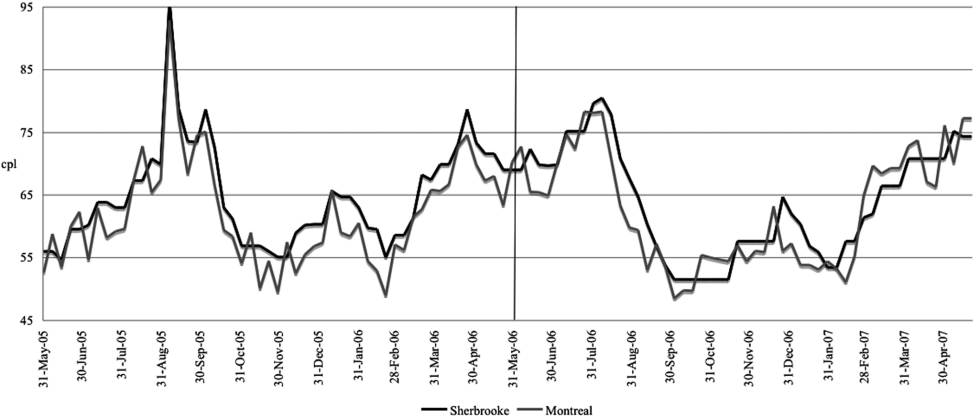
\includegraphics[width=0.92\textwidth]{figures/ch13/erutku2010_fig2.png}
\caption{Weekly retail prices net of taxes in Sherbrooke (black) and Montreal (gray), June 2005 to May 2007, in cents per liter. The
vertical line marks the announcement of the investigation at the end of May 2006. Source: \citet{ErutkuHildebrand2010}, Figure 2.}
\label{fig:13-eh-f2}
\end{figure}

The authors read the Montreal estimate as an overcharge of 1.75 cpl. Relative to the post-announcement Sherbrooke price, this is
$\frac{1.75}{64.0}=2.7$ percent of the retail price. Relative to the post-announcement margin over wholesale cost, it is
$\frac{1.75}{64.0-58.8}=34$ percent. About 135 million liters were sold in Sherbrooke between May 2005 and May 2006, so damages in the year
before the announcement exceed \$2 million ($0.0175\times135$ million $=\$2.4$ million, our arithmetic). The 2.7 percent overcharge is small
next to surveys of cartel overcharges (their Table~7, reproduced in \cref{tab:13-overcharge-surveys}), but the increase in the markup is
large. The authors compare it with Ohio school milk (p.~235). There \citet{PorterZona1999} estimate an average price effect of 6.5
percent, which they translate into a rise of roughly 30 percent in the markup (\cref{sec:13-pz99}). A cartel under investigation may also
keep prices high to reduce estimated damages \citep{Harrington2004}, so the estimate could understate the effect.

\casehead{Critiques}
The design rests on the choice of control. Quebec City matched Sherbrooke in levels before the announcement and moved with it after.
Either Quebec City prices were also affected by the investigation, or the Montreal estimate reflects Montreal-specific shocks. The data
cannot tell these apart. Parallel trends are checked only visually. There is one treated city and one control city in each regression,
so inference treats the weekly observations of a single pair as independent apart from an AR(1) correction. The general problems of
difference in differences with a single treated unit apply (\cref{app:econometrics}). The cartel's end date is uncertain, because
cooperation may have weakened when the wiretaps or raids began. Prices at the end of a cartel need not return at once to the competitive
level. \citet[p.~121]{ClarkHoude2013} report that their companion paper \citep{ClarkHoude2014} finds larger price cuts after the
collapse, which suggests a complementary reading. The cartel's main effect may have been on the shape of the cycle more than on the
average price.

\subsection{Learning to coordinate in Perth: Byrne and de Roos (2019)}\label{sec:13-perth}

The Quebec cartel coordinated by telephone. Coordinating a price increase took on average 65 calls among its members
and a price decrease 26 \citep[pp.~195--196]{AskerNocke2021}. Theory allows firms to reach the same outcome tacitly,
but it says little about how independent firms would arrive at a common understanding (p.~189).
\citet{ByrneDeRoos2019} document such a process in retail gasoline in Perth, Australia, from 2001 to 2015, as
summarized by \citet[pp.~189--191]{AskerNocke2021}. During this period, stations in Perth had to commit to their prices a
day ahead and post them on Fuelwatch, a government website. Its purpose was to help consumers find cheap gasoline.
The same transparency let stations monitor one another, which makes Fuelwatch a form of government-assisted
information sharing like the Danish publication of concrete prices (\cref{sec:13-concrete}).

Perth prices follow cycles of sudden jumps and gradual declines, like those of Toronto (\cref{sec:13-noel}). Before
2009, price jumps occurred on various days of the week. From 2009, BP, the largest chain, led jumps on Wednesdays.
Most of its remaining stations jumped on Thursdays. Caltex, the next-largest chain, gradually adopted the pattern,
and by mid-2010 it followed BP's Wednesday jump with a jump on Thursday. BP then reduced the share of its stations
that jumped on Wednesday and raised the share that jumped on Thursday. It thus scaled back its price leadership, and
with it the sales it lost by leading. In several periods BP stopped leading on Wednesday to test whether the market
would coordinate on Thursday without it (pp.~189--191, Figure~3). Byrne and de Roos identify two focal points
\citep[pp.~596--597 and 607--608]{ByrneDeRoos2019}. The first fixes the timing of the weekly price jump, which moved
to Thursday. The second fixes the size of the daily price cuts between jumps, which converged to 2 cents per liter
from March 2010. By 2013 adjustments were better synchronized and margins were higher.

The episode suggests a third kind of conduct behind similar price cycles. In Toronto the cycles were consistent with
competitive Edgeworth cycles. In Quebec an explicit cartel ran them by telephone. In Perth, the price data show a
detailed pattern of price leadership and price experiments under a transparency regime. The pattern is consistent
with coordination learned through prices. It does not show that prices were the only channel. Byrne and de Roos
state that they cannot rule out explicit communication between firms, such as phone calls
\citep[p.~617]{ByrneDeRoos2019}. Asker and Nocke distill the study as showing that market interaction itself \emph{may}
provide enough communication for coordination (p.~191). In terms of \cref{prop:13-transparency}, Fuelwatch raised the probability
that a deviation would be seen. The transition was slow. Asker and Nocke date it from 2009 to 2013 (p.~189).
Byrne and de Roos describe a gradual three-year transition from April 2009 to August 2012
\citep[p.~592]{ByrneDeRoos2019}, and in their conclusion they speak of three and a half years (p.~618). A simple
rule, such as a fixed day for jumps and a fixed size of cuts, makes deviations easy to detect. It also leaves the firms less able to respond to fluctuations in demand
\citep[p.~194]{AskerNocke2021}. \Cref{sec:12-anatomy} discusses the case as evidence on how agreements start.

\subsection{What the gasoline evidence shows}\label{sec:13-gas-synthesis}

\Cref{tab:13-gas-synthesis} summarizes the five studies. They share an industry, high-frequency prices and an observed wholesale cost.
They differ in what lets them speak about conduct. Borenstein and Shepard use a dynamic implication of the incentive constraint,
the response of margins to expected future demand and cost. Sign restrictions and a placebo separate collusion from inventories and
from measurement error. Noel uses the roles that theory assigns to small and large firms within a cycle. Clark and Houde use wiretaps,
which reveal the conduct directly, and then use structural models to measure what the observed mechanism achieved. Erutku and
Hildebrand use the end of the cartel as an event. Byrne and de Roos follow the emergence of price leadership over time.

\begin{table}[htbp]
\centering
\caption{Retail gasoline studies of conduct}\label{tab:13-gas-synthesis}
\footnotesize
\begin{tabularx}{\textwidth}{>{\raggedright\arraybackslash}p{2.0cm}>{\raggedright\arraybackslash}p{2.3cm}>{\raggedright\arraybackslash}X>{\raggedright\arraybackslash}X>{\raggedright\arraybackslash}X}
\toprule
Study & Market and data & Price pattern & Method & Conclusion about conduct\\
\midrule
\citet{BorensteinShepard1996} & 59 U.S. cities, monthly, 1986--1991 & Margins rise ahead of seasonal demand peaks and fall ahead of cost increases & 2SLS margin regression with forecast demand and cost, elasticity-corrected instrument, placebo on unexpected changes & Tacit dynamic collusion: margin elasticities of 0.37 to expected demand and $-0.37$ to expected cost (Table 2)\\
\addlinespace
\citet{Noel2007} & 22 Toronto stations, twelve-hourly, 131 days in 2001 & Asymmetric weekly cycle: one-step jumps of 5.6 cpl, then 12.8 half-days of small cuts & Markov-switching regression with sticky prices, leader and follower roles by firm type & Competitive Edgeworth cycles: small firms lead cuts, large firms lead relents (Tables II--V)\\
\addlinespace
\citet{ClarkHoude2013} & 128 stations in four Quebec cities, wiretaps 2005--2006, weekly prices 2002--2005 & Asymmetric cycle: increases near 4 cpl, cuts of 1--2 cpl, sticky prices & Coded court documents, delay regressions, logit and homogeneous demand, simulated incentive constraints & Explicit cartel using timed delays as transfers to low-cost firms: 4--6 percent volume gains (Table 7), shorter required punishments (Table 8)\\
\addlinespace
\citet{ErutkuHildebrand2010} & Sherbrooke versus Montreal and Quebec City, weekly, 2005--2007 & Price drop after the announcement of the investigation & Difference in differences with wholesale-price controls and AR(1) errors & Overcharge of 1.75 cpl against Montreal, none against Quebec City (Table 6)\\
\addlinespace
\citet{ByrneDeRoos2019} & Perth, daily station prices posted a day ahead on Fuelwatch, 2001--2015 & Cycles whose jumps moved to Thursdays after 2009 & Event history of price leadership and experimentation by BP & Coordination consistent with signaling through prices, explicit communication not ruled out: weekly jumps on Thursdays, daily cuts of 2 cpl and higher margins by 2013\\
\bottomrule
\end{tabularx}
\end{table}

Three lessons follow. First, price patterns alone do not identify conduct. Asymmetric cycles appear in competitive Toronto and in the
Quebec cartel, and parallel, synchronized increases arise in both. Perth adds cycles that the authors attribute to coordination through prices. Screens based on asymmetry, stickiness or low price variance
\citep{AbrantesMetzEtAl2006} can flag markets for scrutiny, but they cannot separate the two. Second, evidence becomes informative when
it tests a prediction specific to one theory. Examples are the expected-future effects of an incentive constraint, the role
assignments of the Maskin-Tirole equilibrium, or the transfers needed when firms are asymmetric. Third, direct evidence remains decisive
in prosecutions. The Quebec case rested on wiretaps and guilty pleas, and economic analysis then measured the mechanism and its
effects. \Cref{sec:13-enforcement} returns to these methods for measuring damages.

\section{Imperfect Cartels: Tolerated Cheating and Business Stealing}\label{sec:13-imperfect}

The Quebec cartel of \cref{sec:13-clarkhoude} had to shift market share toward the members it needed to keep on
board. The Sugar Institute of \cref{sec:13-sugar-institute} met much of the cheating it detected with
forbearance. Both features recur in the records of prosecuted industrial cartels. The repeated-game theory of
\cref{ch:collusion-theory} explains how the threat of punishment keeps cartel members in line. Its simplest versions make sharp predictions about the records that cartels leave behind.
With perfect monitoring, no member cheats and no punishment occurs on the equilibrium path. With imperfect
public monitoring \citep{GreenPorter1984}, punishments do occur. They are triggered by events that no member
controls, however, and a detected deviation would always be punished. The case records of prosecuted cartels
fit neither prediction. Members cut prices below agreed targets and took customers allocated to others. The
other members knew it, and often nothing followed.

This section documents these facts and recalls the sales-reporting and transfer schemes that cartels used to
contain them (\cref{sec:13-imperfect-evidence}). It then develops the model of \citet{BernheimMadsen2017}, in which
deliberate and unpunished business stealing is part of the optimal cartel agreement (\cref{sec:13-bm}). The
model is the one piece of collusion theory that this chapter develops in full, because its testable
implications concern the internal records of cartels.

\subsection{Evidence from prosecuted industrial cartels}\label{sec:13-imperfect-evidence}

\casehead{The prevalence of discord}
\citet{MarshallMarxSamkharadze2013} classify the European Commission decisions on major industrial cartels
from 2000 to 2005. Throughout this section, page, footnote and theorem numbers for \citet{BernheimMadsen2017}
refer to the working-paper version (NBER Working Paper 19993, 2014). As summarized by
\citet[footnote 2]{BernheimMadsen2017}, Marshall, Marx and Samkharadze label 9 of 22 rulings
\emph{discordant}. In a discordant cartel the decision records frequent bargaining problems and deviations by
members throughout the cartel period. Only 6 rulings are \emph{fully concordant}, meaning that the cartel
functioned smoothly while it lasted. The sample is selected toward cartels effective enough to attract
enforcement. Discord in the population of cartels is therefore probably more common still.
\citet{LevensteinSuslow2006} survey the coordination problems of many cartels and stress the same selection
problem (\cref{ch:collusion-theory}).

\citet[ch.~6]{MarshallMarx2012} offer a first-hand reading of the twenty-two Commission decisions on
industrial-product cartels issued from 2000 through 2005. Following \citet{Stigler1964}, they describe every cartel
as solving the problem of secret deviations with three complementary structures. \emph{Pricing structures} implement price increases. \emph{Allocation structures}
divide the collusive gain and correct deviations through redistributions. \emph{Enforcement structures} monitor
compliance and threaten punishment (pp.~105--106). Their Table~6.1 records the paragraphs of each decision that
describe the cartel's allocation structure and any role of a third-party facilitator (pp.~125--127). By our count
from that table, 17 of the 22 cartels used a market-share allocation, 10 a customer allocation and 7 a geographic
allocation. Nineteen used at least one of the three, and 10 combined market shares with customers or territories.
Eleven decisions mention a facilitator, such as a trade association or a consulting or accounting firm, which can
verify the sales on which a market-share agreement depends (pp.~125 and 128). The vitamins cartel corrected
deviations through ``true-ups''. A firm that sold more than its allotted share had to buy product at the cartel
price from a firm that sold less (p.~128). \citet[p.~198, note~53]{AskerNocke2021} conclude from the same review
that almost all of the decisions feature customer, geographic or market-share allocation.

\casehead{Three cartels in the record}
The global lysine cartel operated at least from 1992 through 1995. Lysine is an amino acid added to animal
feed. Throughout 1993 and 1994 its members discussed a persistent and substantial gap between target and
actual prices in Europe. They first attributed the gap to arbitrage by commodity traders and to exchange
rates, and eventually to undercutting by particular members. The difficulties culminated in a ``reset'', in
which the members briefly suspended sales to drive the price back up to the target. The record shows no
punishment of the deviators \citep[pp.~2--3]{BernheimMadsen2017}. At an April 30, 1993 meeting, the president
of Archer Daniels Midland (ADM) told executives of a Japanese producer that ``our competitors are our friends
and our customers are our enemies.''

A cartel of nucleotide producers (food flavor enhancers) operated in Europe from 1988 to 1999. It tried to
allocate several large customers among its members. At meetings from 1991 to 1996, members complained
repeatedly about low prices and about customers who asked them to match lower quotes from other members.
\citet[p.~3]{BernheimMadsen2017} find no sign that punishments were considered or carried out. Each time, the
cartel set a new price and urged its members to respect it.

The citric acid cartel in western Europe (1991--1995) suspected one member, Jungbunzlauer, of undercutting
during the second half of its life. The members held special sessions alongside the regular meetings to
monitor and discuss Jungbunzlauer's conduct. They never changed the arrangement in response. The cartel
collapsed abruptly in early 1995. Bernheim and Madsen read the collapse as a general breakdown of
coordination and consider a delayed, coordinated punishment the less likely reading. The Sugar Institute of
\cref{sec:13-sugar-institute} shows the same pattern. Members skirted its rules with indirect price cuts or kickbacks,
apologized when caught, and stopped. The Institute then banned the specific practice, and this forbearance
does not seem to have undermined the cartel \citep{GenesoveMullin2001}.

\casehead{Cheating as a defense}
The pattern matters for enforcement. Defendants often present price cuts, business stealing and the absence
of retaliation as proof that a cartel was ineffective. In the criminal trial of ADM executives over lysine, a
defense attorney argued that ADM had been ``stealing customers'' and ``undercutting competitors''
\citep[footnote 10]{BernheimMadsen2017}. In European proceedings, firms in the citric acid, food flavor
enhancer, industrial tube, lysine and zinc phosphate cases argued that agreed prices were not respected and
that non-compliance went unpunished \citep[footnote 11]{BernheimMadsen2017}. A theory in which tolerated
cheating coexists with effective collusion bears directly on how courts should weigh such evidence.

\casehead{Quotas, sales reports and transfers}
Where prices and sales were private, many of these cartels set sales quotas, monitored them through self-reported
sales and settled deviations with interfirm transfers. \Cref{sec:12-hs} documents these schemes, following
\citet{HarringtonSkrzypacz2011}, and \cref{tab:12-hs-allocations} reproduces the quotas of the lysine, citric acid
and 1926 steel cartels. One feature of these schemes matters for the model that follows. In lysine, monthly
``scorecards'' compared each member's reported sales with its quota, and a member above quota had to buy output
from members below it. Some members underreported their sales, yet the agreement was largely successful
\citep[p.~2426]{HarringtonSkrzypacz2011}. Deviations from quota were thus recorded and compensated, and they did
not end the cartel.

Transfer schemes explain how cartels monitor when sales are private. They do not explain why a cartel would
leave detected cheating unpunished. That is the question Bernheim and Madsen answer.

\subsection{A model of imperfect collusion with business stealing}\label{sec:13-bm}

As before, theorem numbers refer to the working-paper version of \citet{BernheimMadsen2017}. We write $\phi$
for the fixed cost of quoting, $\Psi_H$ and $\Psi_A$ for the price distributions of the home and away firms,
and $p^{\mathrm{fl}}$ for the cartel's price floor. Profits are written $\Pi$, as in the paper.

\subsubsection{Environment}

\begin{assumption}[Environment]\label{asm:13-bm}
\leavevmode
\begin{enumerate}[label=(\roman*)]
\item Two risk-neutral firms interact in periods $t=1,2,\dots$ with common discount factor $\delta\in(0,1)$.
There are two markets.
\item Firm $i$ is the \emph{home firm} in market $i$ and the \emph{away firm} in the other market. Its marginal
cost is $c_H$ at home and $c_A$ away, with $\Delta c\equiv c_A-c_H>0$.
\item A firm that quotes a price in a market in a period pays a fixed cost $\phi>0$, whether or not it makes the
sale. The cost stands for a local office, relationships with clients or bid preparation.
\item Each market contains a unit mass of customers with unit demand and reservation values distributed with
CDF $F$. Customers buy from the lowest quote that does not exceed their value, with ties broken at random.
Demand at price $p$ is
\begin{equation}\label{eq:13-bm-demand}
D(p)=1-\lim_{\hat p\uparrow p}F(\hat p).
\end{equation}
\item In each market and period, each firm chooses simultaneously a probability of quoting and a CDF for its
price conditional on quoting. All quotes become public at the end of the period.
\end{enumerate}
\end{assumption}

Two prices summarize each firm's position. The \emph{break-even price} $\underline p_i$, for $i\in\{H,A\}$, is
the lowest price at which a firm that sells to the whole market covers its costs:
\begin{equation}\label{eq:13-bm-breakeven}
\underline p_i=\inf\bigl\{p:\ D(p)(p-c_i)\ge\phi\bigr\}.
\end{equation}
The monopoly price is $p_i^*=\argmax_p D(p)(p-c_i)$. Bernheim and Madsen assume that these prices are unique
and that single-firm profit $D(p)(p-c_i)$ rises strictly between $c_i$ and $p_i^*$. They also assume
$\underline p_A<p_H^*$. Under this condition the low-cost firm cannot blockade entry by charging its monopoly
price. Since $c_A>c_H$, we have $\underline p_H<\underline p_A$ and $p_H^*\le p_A^*$.

Two profit levels serve as benchmarks. The stage profit of a home firm that monopolizes its market at $p_H^*$
is
\begin{equation}\label{eq:13-bm-PiM}
\Pi^M\equiv D(p_H^*)(p_H^*-c_H)-\phi .
\end{equation}
The \emph{competitive profit} is what a home firm earns when it sells to the whole market at the away firm's
break-even price. Since $D(\underline p_A)(\underline p_A-c_A)=\phi$,
\begin{equation}\label{eq:13-bm-PiC}
\Pi^C\equiv D(\underline p_A)(\underline p_A-c_H)-\phi
=D(\underline p_A)(\underline p_A-c_A)+\Delta c\,D(\underline p_A)-\phi=\Delta c\,D(\underline p_A).
\end{equation}
For $\Pi\in[\Pi^C,\Pi^M]$, let $\tilde p(\Pi)$ be the price in $[\underline p_A,p_H^*]$ at which a home
monopolist earns $\Pi$, so that $D(\tilde p)(\tilde p-c_H)-\phi=\Pi$. The map is continuous and strictly
increasing. A final identity links the two firms' profits at the same price. The away firm's single-firm
profit is
\begin{equation}\label{eq:13-bm-identity}
D(p)(p-c_A)-\phi=\bigl[D(p)(p-c_H)-\phi\bigr]-\Delta c\,D(p).
\end{equation}
At the price $\tilde p(\Pi)$, an away firm that takes the whole market earns $\Pi-\Delta c\,D(\tilde p(\Pi))$.

\subsubsection{The stage game}

We first characterize behavior in a single market in which prices below some floor $p_f$ are never quoted.
The same construction delivers both the one-shot equilibrium and, later, optimal collusion.

\begin{lemma}[Indifference construction]\label{lem:13-bm-floor}
Fix $p_f\in[\underline p_A,p_H^*)$. Suppose that in one market the home firm always quotes, with CDF $\Psi_H$
on $[p_f,p_H^*]$. The away firm quotes with probability $\lambda_A$, with an atomless CDF $\Psi_A$ on
$[p_f,p_H^*]$. Suppose further that (a) the away firm earns zero at every price in $(p_f,p_H^*)$ and (b) the
home firm earns the same profit at every price in $[p_f,p_H^*]$. Then
\begin{align}
\Psi_H(p)&=1-\frac{\phi}{D(p)(p-c_A)}\quad\text{for }p\in(p_f,p_H^*),\qquad\Psi_H(p_H^*)=1,
\label{eq:13-bm-psiH}\\
\lambda_A\Psi_A(p)&=1-\frac{D(p_f)(p_f-c_H)}{D(p)(p-c_H)}\quad\text{for }p\in[p_f,p_H^*],
\label{eq:13-bm-psiA}\\
\lambda_A&=1-\frac{D(p_f)(p_f-c_H)}{D(p_H^*)(p_H^*-c_H)} .\label{eq:13-bm-lambda}
\end{align}
The home firm places an atom of mass $1-\frac{\phi}{D(p_f)(p_f-c_A)}$ at $p_f$ and an atom of mass
$\frac{\phi}{D(p_H^*)(p_H^*-c_A)}$ at $p_H^*$. It earns $D(p_f)(p_f-c_H)-\phi$ per period, and the away firm
earns zero.
\end{lemma}

\begin{proof}
An away quote $p\in(p_f,p_H^*)$ wins when the home price exceeds $p$, which has probability $1-\Psi_H(p)$.
Condition (a) reads
\[
\bigl[1-\Psi_H(p)\bigr]D(p)(p-c_A)-\phi=0 .
\]
Solving for $\Psi_H$ gives \eqref{eq:13-bm-psiH}. Letting $p\downarrow p_f$, the probability that the home
price is at most $p_f$ is $1-\frac{\phi}{D(p_f)(p_f-c_A)}$. Since the home firm never quotes below $p_f$, this
is the mass of its atom at $p_f$. Letting $p\uparrow p_H^*$, the probability that the home price is below
$p_H^*$ is $1-\frac{\phi}{D(p_H^*)(p_H^*-c_A)}$. The remaining mass sits at $p_H^*$.

The away firm never quotes $p_f$ or less on this support, so a home quote of $p_f$ wins for sure and earns
$D(p_f)(p_f-c_H)-\phi$. A home quote $p\in(p_f,p_H^*]$ wins unless the away firm quotes and its price is lower,
which has probability $\lambda_A\Psi_A(p)$ because $\Psi_A$ has no atoms. Condition (b) reads
\[
\bigl[1-\lambda_A\Psi_A(p)\bigr]D(p)(p-c_H)-\phi=D(p_f)(p_f-c_H)-\phi .
\]
Solving gives \eqref{eq:13-bm-psiA}. At $p=p_H^*$ the left side of \eqref{eq:13-bm-psiA} must equal
$\lambda_A$, because $\Psi_A(p_H^*)=1$. This gives \eqref{eq:13-bm-lambda}. Both CDFs are nondecreasing
because $D(p)(p-c_A)$ and $D(p)(p-c_H)$ rise on $[\underline p_A,p_H^*]$. The value $\lambda_A$ lies in
$[0,1)$ because $D(p_f)(p_f-c_H)\le D(p_H^*)(p_H^*-c_H)$.
\end{proof}

The probability of \emph{business stealing}, the event that the away firm makes the sale, follows directly.
An away quote $p$ wins with probability $1-\Psi_H(p)=\frac{\phi}{D(p)(p-c_A)}$, so
\begin{equation}\label{eq:13-bm-steal}
\Pr(\text{away firm sells})=\int_{[p_f,\,p_H^*)}\frac{\phi}{D(p)(p-c_A)}\,\dd\bigl[\lambda_A\Psi_A(p)\bigr] .
\end{equation}

\begin{theorem}[Bernheim and Madsen, Theorem 1]\label{thm:13-bm-static}
The stage game has a unique Nash equilibrium. In each market:
\begin{enumerate}[label=(\roman*)]
\item The home firm always quotes. The away firm quotes with probability strictly between 0 and 1.
\item The home firm earns $\Pi^C=\Delta c\,D(\underline p_A)>0$, and the away firm earns zero.
\item Prices lie in $[\underline p_A,p_H^*]$. Each firm's price distribution has full support on this interval
and is atomless, except for an atom of the home firm at $p_H^*$.
\end{enumerate}
The equilibrium distributions are those of \cref{lem:13-bm-floor} with $p_f=\underline p_A$.
\end{theorem}

\begin{proof}[Proof of equilibrium, with uniqueness in outline]
Set $p_f=\underline p_A$ in \cref{lem:13-bm-floor}. The home atom at $\underline p_A$ has mass
$1-\frac{\phi}{D(\underline p_A)(\underline p_A-c_A)}=0$, and the home profit is
$D(\underline p_A)(\underline p_A-c_H)-\phi=\Pi^C$ by \eqref{eq:13-bm-PiC}. We check that neither firm gains
by leaving its support.

Consider the away firm. It earns zero at every price in $[\underline p_A,p_H^*)$. A price above $p_H^*$ never
wins and costs $\phi$. A price below $\underline p_A$ yields at most $D(p)(p-c_A)-\phi<0$. Staying out yields
zero. Mixing between quoting and staying out is therefore optimal.

Consider the home firm. It earns $\Pi^C$ at every price in $[\underline p_A,p_H^*]$. A price below
$\underline p_A$ also wins for sure but earns less, since $D(p)(p-c_H)$ rises below $p_H^*$. A price
$p>p_H^*$ wins only if the away firm stays out and earns
$(1-\lambda_A)D(p)(p-c_H)-\phi<(1-\lambda_A)D(p_H^*)(p_H^*-c_H)-\phi=\Pi^C$. Staying out earns $0<\Pi^C$.

Uniqueness is proved in Appendix B of the working paper (Theorem B.1 and Lemmas B.1 to B.7). The steps show
that both firms' supports end at $p_H^*$, that equilibrium prices lie in $[\underline p_A,p_H^*]$, and that
the only possible atom is the home firm's atom at $p_H^*$. Given these facts, conditions (a) and (b) of
\cref{lem:13-bm-floor} must hold, and they pin down the distributions.
\end{proof}

Three features of this equilibrium stand out \citep[p.~9]{BernheimMadsen2017}. First, customers always pay
strictly more than $\underline p_A$, the lowest price the high-cost firm would ever accept. Expected profits
are the same as if both firms quoted $\underline p_A$ and the home firm sold, yet prices are higher, because
both firms pay fixed costs. Second, prices have full support up to $p_H^*$, so an ex post outcome can look
arbitrarily collusive. Third, business stealing occurs with positive probability even though there is no
cartel.

\begin{example}[Uniform values]\label{ex:13-bm-uniform}
Let $v\sim U[0,1]$, so $D(p)=1-p$, with $c_H=0.1$, $c_A=0.2$ and $\phi=0.05$. The home monopoly price solves
$\frac{\dd}{\dd p}(1-p)(p-0.1)=1.1-2p=0$, so $p_H^*=0.55$. The away break-even price is the lower root of
\[
(1-p)(p-0.2)=0.05\iff p^2-1.2p+0.25=0,
\]
which gives $\underline p_A=\frac{1.2-\sqrt{0.44}}{2}\approx 0.2683$. The assumption $\underline p_A<p_H^*$
holds. The benchmarks are $\Pi^C=0.1\times(1-0.2683)=0.0732$ and $\Pi^M=0.45\times0.45-0.05=0.1525$. By
\eqref{eq:13-bm-psiH}, $\Psi_H(p)=1-\frac{0.05}{(1-p)(p-0.2)}$, with an atom of
$\frac{0.05}{0.45\times0.35}=0.3175$ at $p_H^*$. The numerator of \eqref{eq:13-bm-psiA} is
$D(\underline p_A)(\underline p_A-c_H)=\Pi^C+\phi=0.1232$, so
\[
\lambda_A\Psi_A(p)=1-\frac{0.1232}{(1-p)(p-0.1)},\qquad \lambda_A=1-\frac{0.1232}{0.2025}=0.3918 .
\]
Evaluating \eqref{eq:13-bm-steal} numerically, the away firm makes the sale with probability $0.238$. The
expected lowest quote is $0.368$, against a break-even price of $0.268$. Panel (a) of \cref{fig:13-bm-cdfs}
plots the two distributions.
\end{example}

\begin{figure}[htbp]
\centering
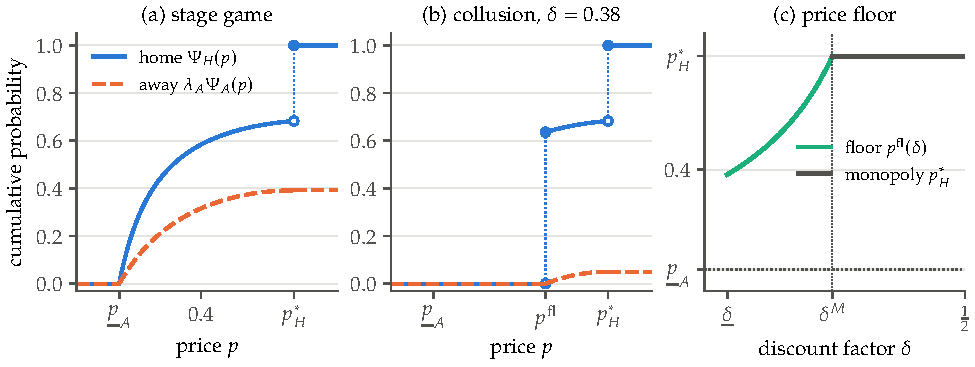
\includegraphics[width=\textwidth]{figures/ch13/bm_cdfs.pdf}
\caption{The model of \citet{BernheimMadsen2017} with $v\sim U[0,1]$, $c_H=0.1$, $c_A=0.2$ and $\phi=0.05$.
Panels (a) and (b) show the home firm's price CDF $\Psi_H$ as a solid line, with atoms marked by dots. The dashed
line is the away firm's unconditional CDF of quotes $\lambda_A\Psi_A$, which ends at the entry probability
$\lambda_A$.
Panel (a) is the stage-game equilibrium. Panel (b) is the optimal stationary collusive equilibrium at
$\delta=0.38$, with floor $p^{\mathrm{fl}}=0.449$. Panel (c) shows the floor $p^{\mathrm{fl}}(\delta)$ over
$[\underline\delta,\delta^M]=[0.345,0.413]$, where $\underline\delta=\delta^0$ is the threshold of
\cref{thm:13-bm-punish}. Above $\delta^M$ the cartel achieves the monopoly price. Source: our calculations
(\texttt{bm\_static.py}).}
\label{fig:13-bm-cdfs}
\end{figure}

\subsubsection{Stationary collusion}

Industry profit is highest when each home firm monopolizes its market at $p_H^*$ and the away firm stays out.
We call this \emph{perfect collusion}. An equilibrium with profits above the stage-game level and below
perfect collusion is an \emph{imperfectly collusive} arrangement. Lifetime profits are normalized as
$(1-\delta)\sum_{t\ge1}\delta^{t-1}\pi_t$, so that a constant stream $\pi$ is worth $\pi$. Characterizing the
whole equilibrium payoff set of a repeated game with mixed strategies and continuous actions is hard.
Bernheim and Madsen therefore restrict attention to the following class.

\begin{definition}[Stationary equilibrium]\label{def:13-bm-stationary}
A subgame perfect equilibrium is \emph{stationary} if there is a stage-game strategy profile $\tau$ such that
$\tau$ is played after every history on the equilibrium path. Behavior off the path is unrestricted beyond
subgame perfection.
\end{definition}

Off-path behavior can be nonstationary, so optimal penal codes in the sense of \citet{Abreu1988} are allowed.
On the path, lifetime profits equal stage profits. Let $\underline\Pi(\delta)$ be the infimum of a firm's
lifetime profits over all subgame perfect equilibria, and let $\delta^M$ be the lowest discount factor at which
perfect collusion is sustainable.

\begin{theorem}[Bernheim and Madsen, Theorem 2]\label{thm:13-bm-optimal}
For each $\delta\le\delta^M$, the unique Pareto-optimal stationary equilibrium profit vector
$(\bar\Pi,\bar\Pi)$ satisfies
\begin{equation}\label{eq:13-bm-thm2}
\bar\Pi=(1-\delta)\Bigl[2\bar\Pi-\Delta c\,D\bigl(\tilde p(\bar\Pi)\bigr)\Bigr]+\delta\,\underline\Pi(\delta).
\end{equation}
Moreover, $\bar\Pi>\Pi^C$ if and only if $\underline\Pi(\delta)<\Pi^C$, and $\bar\Pi$ is strictly increasing in
$\delta$ whenever $\underline\Pi(\cdot)$ is nonincreasing.
\end{theorem}

We derive the incentive constraint behind \eqref{eq:13-bm-thm2}. Consider an agreement that divides the
markets along cost lines and gives each firm stage profit $\Pi$ in its home market. The rival's lowest home
price $p_{\min}$ must satisfy $D(p_{\min})(p_{\min}-c_H)-\phi\ge\Pi$, since even a sure sale at the lowest price
must deliver $\Pi$. Hence $p_{\min}\ge\tilde p(\Pi)$. Consider a firm that keeps its home strategy and
slightly undercuts $p_{\min}$ in the away market for one period.
\begin{enumerate}[label=Step \arabic*.,leftmargin=*]
\item By \eqref{eq:13-bm-identity}, undercutting $p_{\min}$ in the away market earns
\[
D(p_{\min})(p_{\min}-c_A)-\phi=\bigl[D(p_{\min})(p_{\min}-c_H)-\phi\bigr]-\Delta c\,D(p_{\min})
\ge\Pi-\Delta c\,D\bigl(\tilde p(\Pi)\bigr),
\]
because the bracket is at least $\Pi$ and $D(p_{\min})\le D(\tilde p(\Pi))$.
\item Adding the home profit $\Pi$, the deviation earns at least $2\Pi-\Delta c\,D(\tilde p(\Pi))$ in the
deviation period.
\item The worst the cartel can do afterwards is to impose $\underline\Pi(\delta)$. The deviator's lifetime payoff
is at least
\[
(1-\delta)\Bigl[2\Pi-\Delta c\,D\bigl(\tilde p(\Pi)\bigr)\Bigr]+\delta\,\underline\Pi(\delta).
\]
\item The agreement survives only if the on-path payoff is at least this large:
\begin{equation}\label{eq:13-bm-ic}
\Pi\ \ge\ (1-\delta)\Bigl[2\Pi-\Delta c\,D\bigl(\tilde p(\Pi)\bigr)\Bigr]+\delta\,\underline\Pi(\delta).
\end{equation}
\item The firms pick the largest $\Pi$ that satisfies \eqref{eq:13-bm-ic}. At that $\Pi$ the constraint
binds, which is \eqref{eq:13-bm-thm2}. The equilibrium of \cref{thm:13-bm-structure} below attains it.
\end{enumerate}
Both firms agree on the best scheme, so the Pareto frontier of stationary equilibria is a single symmetric
point.

\begin{remark}[Nash reversion supports no collusion]\label{rem:13-bm-nash}
Collusion in this model requires punishments harsher than reversion to the stage game
\citep[footnote 22]{BernheimMadsen2017}. To see why, set $\underline\Pi=\Pi^C$ in \eqref{eq:13-bm-ic} and
subtract $\Pi^C$ from both sides:
\[
\Pi-\Pi^C\ \ge\ (1-\delta)\Bigl[2\Pi-\Delta c\,D(\tilde p)-\Pi^C\Bigr]
=(1-\delta)\bigl[(\Pi-\Pi^C)+a(\tilde p)\bigr],
\]
where $a(p)\equiv D(p)(p-c_A)-\phi=\Pi-\Delta c\,D(\tilde p)$ at $p=\tilde p(\Pi)$ is the away firm's
single-firm profit. Rearranging gives $\delta(\Pi-\Pi^C)\ge(1-\delta)\,a(\tilde p)$. Now
$\Pi-\Pi^C=a(\tilde p)-\Delta c\bigl[D(\underline p_A)-D(\tilde p)\bigr]\le a(\tilde p)$. The constraint
therefore requires $\delta\,a(\tilde p)\ge(1-\delta)\,a(\tilde p)$, that is, $\delta\ge\frac{1}{2}$. Since
$\delta^M<\frac{1}{2}$ (\cref{thm:13-bm-perfect}), Nash reversion sustains no profit above $\Pi^C$ in the whole
range where imperfect collusion is the relevant case.
\end{remark}

\begin{theorem}[Bernheim and Madsen, Theorem 3]\label{thm:13-bm-punish}
Suppose
\[
\delta\ \ge\ \delta^0\equiv\frac{1}{2+\frac{\Delta c\,D(p_H^*)}{\phi}} .
\]
Then a subgame perfect equilibrium gives both firms zero lifetime profits, so $\underline\Pi(\delta)=0$.
\end{theorem}

Zero is the harshest conceivable punishment, because a firm can always stay out of both markets. The
punishment is a one-period price war followed by a return to optimal collusion. In the war period both firms
enter both markets. The home firm quotes some $p^{PW}\le\underline p_H$ and serves its market at a loss. The
away firm mixes over $(p^{PW},\underline p_H]$, never sells, and loses its fixed cost. Its presence ensures
that a home firm that raises its price cannot profit. If both firms take part, play returns to the
collusive phase worth $\bar\Pi$. If either refuses, the war restarts. The war price is set so that
\[
(1-\delta)\Bigl[D(p^{PW})(p^{PW}-c_H)-2\phi\Bigr]+\delta\bar\Pi=0 .
\]
The bound on $\delta$ guarantees $p^{PW}\le\underline p_H$. A deviator's best option in the war period is then
to exit both markets, which yields zero today and a restarted war, so it gains nothing.

\begin{theorem}[Bernheim and Madsen, Theorem 4]\label{thm:13-bm-perfect}
Suppose $\Pi^M>\phi+\Delta c\,D(p_H^*)$. Then $\delta^0<\delta^M$, and for each $\delta\in[\delta^0,\delta^M]$
the optimal stationary profit satisfies
\begin{equation}\label{eq:13-bm-thm4}
\bar\Pi=(1-\delta)\Bigl[2\bar\Pi-\Delta c\,D\bigl(\tilde p(\bar\Pi)\bigr)\Bigr].
\end{equation}
The profit $\bar\Pi$ is continuous, strictly greater than $\Pi^C$, and strictly increasing in $\delta$. Perfect
collusion is sustainable for all $\delta\ge\delta^M$, where
\begin{equation}\label{eq:13-bm-deltaM}
\delta^M=\frac{\Pi^M-\Delta c\,D(p_H^*)}{2\Pi^M-\Delta c\,D(p_H^*)} .
\end{equation}
\end{theorem}

The threshold \eqref{eq:13-bm-deltaM} follows from \eqref{eq:13-bm-ic}. Perfect collusion sets $\Pi=\Pi^M$,
so $\tilde p(\Pi^M)=p_H^*$, and the harshest punishment is zero:
\begin{align*}
\Pi^M&\ge(1-\delta)\bigl[2\Pi^M-\Delta c\,D(p_H^*)\bigr]\\
1-\delta&\le\frac{\Pi^M}{2\Pi^M-\Delta c\,D(p_H^*)}\\
\delta&\ge1-\frac{\Pi^M}{2\Pi^M-\Delta c\,D(p_H^*)}=\frac{\Pi^M-\Delta c\,D(p_H^*)}{2\Pi^M-\Delta c\,D(p_H^*)} .
\end{align*}
The numerator is the away firm's profit at $p_H^*$, which is positive because $p_H^*>\underline p_A$. Twice the
numerator, $2\Pi^M-2\Delta c\,D(p_H^*)$, is smaller than the denominator, so $\delta^M<\frac{1}{2}$. In the
symmetric Bertrand duopoly without fixed costs the threshold is exactly $\frac{1}{2}$ (\cref{ch:collusion-theory}).
Here a raid on the other market earns less than the home firm's profit, because the raider has the higher
cost. The temptation is smaller, so perfect collusion is easier.

For $\delta\in[\delta^0,\delta^M)$, equation \eqref{eq:13-bm-thm4} pins down the floor
$p^{\mathrm{fl}}(\delta)\equiv\tilde p(\bar\Pi(\delta))$. Collecting terms in \eqref{eq:13-bm-thm4} gives
$(1-2\delta)\bar\Pi=(1-\delta)\Delta c\,D(\tilde p(\bar\Pi))$, which in terms of the floor reads
\begin{equation}\label{eq:13-bm-floor}
(1-2\delta)\Bigl[D(p^{\mathrm{fl}})(p^{\mathrm{fl}}-c_H)-\phi\Bigr]=(1-\delta)\,\Delta c\,D(p^{\mathrm{fl}}) .
\end{equation}
The left side rises in $p^{\mathrm{fl}}$ and the right side falls. At $\underline p_A$ the left side minus the
right side equals $(1-2\delta)\Pi^C-(1-\delta)\Pi^C=-\delta\Pi^C<0$. At $p_H^*$ it equals
$(1-2\delta)\Pi^M-(1-\delta)\Delta c\,D(p_H^*)$, which is positive exactly when $\delta<\delta^M$. A unique
floor therefore lies strictly between $\underline p_A$ and $p_H^*$. Differentiating the difference with
respect to $\delta$ gives $-2\Pi+\Delta c\,D(p)=-[\Pi+a(p)]<0$. By the implicit function theorem the floor
rises with $\delta$ and reaches $p_H^*$ at $\delta^M$.

\begin{theorem}[Bernheim and Madsen, Theorem 5]\label{thm:13-bm-structure}
When $\delta<\delta^M$, the profits $(\bar\Pi,\bar\Pi)$ are supported by a stationary equilibrium with the
following on-path properties:
\begin{enumerate}[label=(\roman*)]
\item The home firm's strategy is the same in each market, and so is the away firm's.
\item The home firm always enters. The away firm enters with probability strictly between 0 and 1.
\item The home firm earns stage profit $\bar\Pi$, and the away firm earns zero.
\item Each firm's price distribution has full support on $[p^{\mathrm{fl}},p_H^*]$. The home firm places atoms
at $p^{\mathrm{fl}}$ and at $p_H^*$. The away firm's distribution is continuous.
\item The away firm sells with positive probability, which decreases in $\bar\Pi$.
\item An away quote at or below $p^{\mathrm{fl}}$ triggers a punishment worth $\underline\Pi(\delta)$ to the
deviator.
\end{enumerate}
These on-path strategies are unique among stationary equilibria whose price distributions have full support on
$[p^{\mathrm{fl}},p_H^*]$.
\end{theorem}

The on-path strategies are exactly those of \cref{lem:13-bm-floor} with $p_f=p^{\mathrm{fl}}$, as the proof
of Theorem B.4 in the working paper confirms. The equilibrium check is short. The away firm earns zero at
every price in $(p^{\mathrm{fl}},p_H^*)$ and is never punished there. Its best one-period deviation is to
undercut the home atom at $p^{\mathrm{fl}}$, which earns $\bar\Pi-\Delta c\,D(p^{\mathrm{fl}})$ by
\eqref{eq:13-bm-identity}. The home firm earns $\bar\Pi$ at every price it quotes, so it cannot gain at home.
A firm that combines both moves earns $2\bar\Pi-\Delta c\,D(p^{\mathrm{fl}})$ for one period and then
$\underline\Pi(\delta)$. Condition \eqref{eq:13-bm-thm2} says that this deviation exactly breaks even. The
stage equilibrium of \cref{thm:13-bm-static} is the special case $p^{\mathrm{fl}}=\underline p_A$, in which the
home atom at the floor vanishes.

\begin{example}[Uniform values, continued]\label{ex:13-bm-uniform-coll}
In \cref{ex:13-bm-uniform}, $\Delta c\,D(p_H^*)=0.1\times0.45=0.045$ and $\Pi^M=0.1525>\phi+0.045=0.095$, so
\cref{thm:13-bm-perfect} applies. The thresholds are
\[
\delta^0=\frac{1}{2+\frac{0.045}{0.05}}=\frac{1}{2.9}=0.345,\qquad
\delta^M=\frac{0.1525-0.045}{0.305-0.045}=\frac{0.1075}{0.26}=0.413 .
\]
At $\delta=0.38$, equation \eqref{eq:13-bm-floor} gives $p^{\mathrm{fl}}=0.449$ and $\bar\Pi=0.142$. The home
firm quotes the floor with probability $0.636$ and the monopoly price with probability $0.317$. The away firm
enters with probability $\lambda_A=0.050$ and makes the sale with probability $0.017$, down from $0.238$ in the
stage game. The expected lowest quote is $0.482$. A clean split of the markets at the floor would give the
same profits with a price of $0.449$, so the tolerated raids cost consumers money. Panels (b) and (c) of
\cref{fig:13-bm-cdfs} show the distributions and the floor as a function of $\delta$.
\end{example}

\subsubsection{Why the cartel tolerates raids}

Why do the firms not agree on the simpler plan of a clean split at the floor? Under a clean split the away
firm stays out, and the home firm sells at $p^{\mathrm{fl}}$. A firm could then raise its home price to $p_H^*$
and raid the other market at the same time. If no business stealing ever occurs on the path, the best
deviation earns $\Pi^M$ at home plus $\Pi-\Delta c\,D(\tilde p(\Pi))$ away. The agreement is incentive
compatible only if
\begin{equation}\label{eq:13-bm-nosteal}
\Pi\ \ge\ (1-\delta)\Bigl[\Pi-\Delta c\,D\bigl(\tilde p(\Pi)\bigr)+\Pi^M\Bigr]+\delta\,\underline\Pi(\delta).
\end{equation}
The deviation payoff here exceeds the one in \eqref{eq:13-bm-ic} by $(1-\delta)(\Pi^M-\Pi)>0$. At
$\Pi=\bar\Pi$ the constraint \eqref{eq:13-bm-ic} binds, so \eqref{eq:13-bm-nosteal} fails. All punishment
power is already used to deter raids, so none is left to deter the home price increase. The cartel must
instead make a high home price unattractive directly. It does so by letting the away firm enter at prices
above the floor. Entry costs $\phi$, so the away firm enters only if it sometimes wins. The home firm cedes
those sales by charging the monopoly price part of the time. Equilibrium thus combines occasional price
escalation at home with unpunished business stealing away \citep[pp.~15--17]{BernheimMadsen2017}.

\begin{theorem}[Bernheim and Madsen, Theorems 6 and 7]\label{thm:13-bm-inevitable}
Let $\delta<\delta^M$.
\begin{enumerate}[label=(\roman*)]
\item All stationary equilibria with profits $(\bar\Pi,\bar\Pi)$ share the same minimum price, maximum price and
entry probabilities. Among them, the equilibrium of \cref{thm:13-bm-structure} uniquely minimizes the
probability that an away firm wins.
\item There exists $\tilde\Pi<\bar\Pi$ such that in any stationary equilibrium with profits
$(\Pi_1,\Pi_2)>(\tilde\Pi,\tilde\Pi)$, the away firm captures each market with strictly positive probability on
the equilibrium path.
\end{enumerate}
\end{theorem}

Part (ii) follows from \eqref{eq:13-bm-nosteal} by continuity. The constraint fails at $\bar\Pi$, and both
sides are continuous in $\Pi$, so it fails on an interval of profits below $\bar\Pi$. Business stealing is
therefore a feature of every nearly optimal cartel. It is not an artifact of a particular equilibrium.

\begin{remark}[Why tolerate deliberate cheating?]\label{rem:13-bm-puzzle}
The model resolves the puzzle posed by the lysine, nucleotide and citric acid records. When perfect collusion
is out of reach, every member knows that the aspirational price cannot hold. Members protect their home markets
by occasionally cutting price to the floor, and they raid each other at prices above it. The raids are
anticipated and serve a purpose. Their threat keeps home prices from drifting up to levels that would make the
cartel unstable. Punishing them would remove that discipline. Only raids at or below the floor, which the
home firm could have prevented by quoting the floor, would be punished.
\end{remark}

\casehead{Testable implication}
The cleanest prediction is that business stolen at prices above the floor goes unpunished, while stealing below
the floor triggers punishment. The floor is rarely known with precision. The average price is no proxy for it,
because some stealing occurs at below-average prices. Bernheim and Madsen therefore propose a more robust
implication: the higher the price at which business is stolen, the less likely the theft is to trigger
punishment. They leave the test to future work \citep[p.~7]{BernheimMadsen2017}.

\casehead{Many firms and comparative statics}
With $N+1$ firms and $N+1$ markets, the stage game has many equilibria. For each nonempty set of away firms
there is a unique equilibrium in which exactly those firms enter (Theorem 8). Bernheim and Madsen then restrict
attention to \emph{market-symmetric} equilibria, in which all away firms in a market play alike. Under mild
conditions on $N$ and $\Pi^M$ they obtain analogues of the duopoly results (Theorems 9 to 13). Optimal profits
satisfy
$\bar\Pi=(1-\delta)\bigl[(N+1)\bar\Pi-\Delta c\,N\,D(\tilde p(\bar\Pi))\bigr]+\delta\,\underline\Pi(\delta;N)$,
because a deviator keeps its home profit and raids all $N$ other markets. The perfect-collusion threshold is
\[
\delta^M(N)=1-\frac{1}{N+1}\left(\frac{N}{N+1}\,\frac{\tilde\Pi^M}{\Pi^M}+\frac{1}{N+1}\right)^{-1},
\]
where $\tilde\Pi^M=\Pi^M-\Delta c\,D(p_H^*)$ is a high-cost firm's profit at $p_H^*$. With $N=1$ the formula
reduces to \eqref{eq:13-bm-deltaM}. The threshold lies below $1-\frac{1}{N+1}$, rises with $N$ and tends to one
(Theorem 14). Large cartels can therefore hope only for imperfect collusion, even when their members are very
patient. The two frictions are both needed. As $c_A\to c_H$, collusion becomes all or nothing: $\bar\Pi\to\Pi^C$
for $\delta<\frac{N}{N+1}$ and $\bar\Pi\to\Pi^M$ for $\delta\ge\frac{N}{N+1}$ (Theorem 15). As $\phi\to0$,
business stealing vanishes and the home firm sells at $\underline p_A$ with probability one (Theorem 16).

\casehead{Assessment}
The model explains two facts that standard theory does not, deliberate cheating and its toleration, without
any monitoring noise. Several features limit its reach. The analysis is confined to stationary equilibria,
and the authors cannot rule out that nonstationary schemes do better. In the duopoly $\delta^M<\frac{1}{2}$, so
with literal discounting perfect collusion would be easy. Bernheim and Madsen therefore read $\delta$ as a
reduced form for impatience from agency problems, turnover or the number of rivals, and the many-firm results
support that reading. The sharp divide between tolerated and punished stealing would blur with imperfect
monitoring, for example with rogue salespeople who do not know about the cartel. The theory's main empirical
implication has not yet been tested. Read together, \citet{HarringtonSkrzypacz2011} and
\citet{BernheimMadsen2017} show that the internal records of cartels contain more than evidence of agreement.
Quotas, reports, transfers and tolerated raids are equilibrium objects with testable structure. The next
section studies a cartel whose internal records are complete enough to estimate such structure.

\section{Inside a Bidding Ring: Asker's Stamp Cartel}\label{sec:13-asker}

A bidding ring is a cartel of bidders. \Cref{sec:14-collusion} shows that in an English auction a ring
whose members know each other's values is self-enforcing (\cref{prop:14-robinson}). Real rings do not know
their members' values. They must elicit them and divide the gains, and the mechanism they use shapes both
bidding and damages. \citet{Asker2010} studies a ring of stamp dealers whose internal records survive in full.
His questions are how the ring organized itself, what incentives its mechanism created, and who bore the costs:
sellers, bidders outside the ring, or the ring itself. The answers matter for antitrust damages, for the
efficiency costs of collusion, and for detection, which relies on understanding how rings behave in practice.

\subsection{Question and institutions}\label{sec:13-asker-institutions}

Until July 1997, 11 wholesale stamp dealers belonged to the ring. It bid in auctions of collectible stamps,
typically collections, held mainly at New York auction houses. These houses ran open outcry ascending
auctions, that is, English auctions. The ring began in the late 1970s or early 1980s and lasted 15 to 20 years,
with very few changes in membership after its first five years. It collapsed when a stamp dealer outside the
ring brought it to the attention of antitrust enforcers \citep[p.~725]{Asker2010}. The data come from the
resulting case, \textit{New York et al.\ v.\ Feldman et al.}\ in the Southern District of New York.

\casehead{The knockout}
The ring coordinated through a \emph{knockout}, a private auction held before each \emph{target auction}.
Members sent sealed bids on the lots they wanted, by fax or in writing, to an agent: a New York taxi and
limousine driver employed by the ring. The agent determined the winner of each lot and notified the members.
He sent the bids to another member, who computed the sidepayments after the target auction. Sidepayments were
aggregated and settled quarterly. In the target
auction the agent, or another agent he arranged, bid for the knockout winner up to the winning knockout bid.
The winning bid thus set the ring's bidding limit. Because the ring's own agent did the bidding, compliance
with the limit was easy to monitor. The coordinating member paid the agent \$30 an hour, and each member paid
him \$50 for every target auction in which it was active. Depositions state that the agent never revealed bids
before a knockout closed. Ties were resolved by the agent, who tried ``as much as possible to be fair''
\citep[pp.~727--728]{Asker2010}.

\casehead{Enforcement}
Evidence on enforcement is thin. In the ring's early years at least two members were expelled, one for not
meeting his financial obligations and one for being interested only in sidepayments. The records show no member
who lost a knockout and then bid against the ring, and no temporary suspensions. One auction house signaled
that it knew a ring was active, and the ring stopped operating there. In its final years the ring hid its
activity by also bidding through other professional agents and through its own members
\citep[p.~728]{Asker2010}.

Knockouts of the kind this ring used have a long history in markets for rare books, art, rugs, stamps, coins
and antiques. In the 1919 sale of the library of Ruxley Lodge in England, 81 London booksellers formed a ring.
Their knockouts after the sale ran in rounds of 81, 24, 15 and finally 8 members. These rounds raised
\pounds10,292 on top of the \pounds3,161 paid in the sale itself. Rings were legal in the United Kingdom before
1927 \citep[p.~726]{Asker2010}.

\casehead{The sidepayment rule}
Sidepayments compensated members for not competing when the ring won. Let $P$ be the target price paid by the
ring. Order the knockout bids from highest to lowest as $b_{(1)}\ge b_{(2)}\ge\dots\ge b_{(n)}$. Here the
subscript counts from the top, unlike the order statistics of \cref{ch:auction-theory}. Let $m$ be the number
of bids at or above $P$, and set $b_{(m+1)}\equiv P$.

\begin{definition}[Incremental sidepayment rule]\label{def:13-asker-rule}
For $j=2,\dots,m$, let $\Delta_j=b_{(j)}-b_{(j+1)}$ be the increment between consecutive eligible bids. The
knockout winner keeps half of each increment. The other half is split equally among the $j-1$ losing bidders
whose bids are at least $b_{(j)}$. Bidders with bids below $P$ receive nothing.
\end{definition}

\begin{proposition}[Properties of the rule]\label{prop:13-asker-sidepay}
Under \cref{def:13-asker-rule}:
\begin{enumerate}[label=(\roman*)]
\item The loser ranked $k\in\{2,\dots,m\}$ receives $s_{(k)}=\sum_{j=k}^{m}\frac{\Delta_j}{2(j-1)}$.
\item The winner pays $\frac{1}{2}\bigl(b_{(2)}-P\bigr)$ in total. Its outlay for the lot is
$P+\frac{1}{2}(b_{(2)}-P)=\frac{1}{2}(P+b_{(2)})$.
\item Payments balance.
\item Holding ranks fixed, a loser's receipt rises by $\frac{1}{2(k-1)}$ per dollar of its own bid whenever its
bid exceeds $P$.
\item With two knockout bidders, the loser receives $\frac{1}{2}(b_{(2)}-P)^+$.
\end{enumerate}
\end{proposition}

\begin{proof}
Part (i) restates the rule: the loser ranked $k$ shares in increments $j=k,\dots,m$, each among $j-1$ losers.
For (ii), the winner pays half of every increment, and the sum telescopes:
\[
\sum_{j=2}^{m}\frac{\Delta_j}{2}=\frac{1}{2}\bigl(b_{(2)}-b_{(m+1)}\bigr)=\frac{1}{2}\bigl(b_{(2)}-P\bigr) .
\]
For (iii), exchange the order of summation in the losers' receipts:
\[
\sum_{k=2}^{m}s_{(k)}=\sum_{j=2}^{m}\ \sum_{k=2}^{j}\frac{\Delta_j}{2(j-1)}=\sum_{j=2}^{m}\frac{\Delta_j}{2}
=\frac{1}{2}\bigl(b_{(2)}-P\bigr) .
\]
For (iv), the own bid $b_{(k)}$ enters $s_{(k)}$ only through $\Delta_k=b_{(k)}-b_{(k+1)}$, with weight
$\frac{1}{2(k-1)}$. Part (v) is the case $m=2$.
\end{proof}

\begin{remark}[The rule for any number of eligible reports]\label{rem:13-mm-table91}
\citet[pp.~192--194, Table~9.1]{MarshallMarx2012} state the ring's payments for any number of eligible reports. They
rank the reports as $r_1 > r_2 > \dots > r_k > p > r_{k+1} > \dots > r_n$, where $p$ is the price paid at the
auction. In our notation $r_j = b_{(j)}$, $p = P$ and $k = m$. Members $k+1, \dots, n$ receive nothing. Member $k$
receives $\frac{r_k - p}{2}\cdot\frac{1}{k-1}$, member 2 receives
\begin{equation*}
  \frac{r_k - p}{2}\cdot\frac{1}{k-1} + \frac{r_{k-1} - r_k}{2}\cdot\frac{1}{k-2} + \dots + \frac{r_2 - r_3}{2} ,
\end{equation*}
and member 1, the winner, pays the sum of the half-increments, $\frac{r_k - p}{2} + \frac{r_{k-1} - r_k}{2} + \dots
+ \frac{r_2 - r_3}{2}$. Since $r_j - r_{j+1} = \Delta_j$, these are parts (i) and (ii) of \cref{prop:13-asker-sidepay}.
Their verbal summary is \citeauthor{Asker2010}'s description of \cref{def:13-asker-rule}, and they call the mechanism a
variant of the one described by \citet{GrahamMarshallRichard1990} (p.~193, note~15). They also note that members
have an incentive to overreport, which the ring accepted as a cost of doing business, much as cartels accept some
misreporting of sales (p.~194).
\end{remark}

\begin{example}[Sotheby's, June 24, 1997, Lot 49]\label{ex:13-asker-ko}
\Cref{tab:13-asker-ex1} reproduces Asker's Example 1. Bidder J's \$5,100 lies below the target price of
\$6,750, so J is not eligible and $m=3$. The increments are $\Delta_3=7{,}500-6{,}750=750$ and
$\Delta_2=8{,}000-7{,}500=500$. Bidder A keeps \$375 of the first increment and gives \$187.50 each to B and G.
A keeps \$250 of the second increment and gives \$250 to G, the only loser whose bid reaches \$8,000. A pays
$\frac{1}{2}(8{,}000-6{,}750)=625$, which equals $437.50+187.50$. A's outlay is \$7,375 for a lot bought at
\$6,750. \Cref{fig:13-asker-numberline} shows the increments.
\end{example}

\begin{table}[htbp]
\centering
\caption{Sidepayments after a successful acquisition: Sotheby's, June 24, 1997, Lot 49}
\label{tab:13-asker-ex1}
\begin{threeparttable}
\begin{tabular}{@{}lrl@{}}
\toprule
Knockout auction & Bid (\$) & Sidepayment (\$) \\
\midrule
Bidder A & 9,000 & $-\left(\frac{7{,}500-6{,}750}{2}\right)-\left(\frac{8{,}000-7{,}500}{2}\right)=-625$ \\[6pt]
Bidder G & 8,000 & $+\left(\frac{7{,}500-6{,}750}{2}\right)\times\frac{1}{2}+\left(\frac{8{,}000-7{,}500}{2}\right)=437.50$ \\[6pt]
Bidder B & 7,500 & $+\left(\frac{7{,}500-6{,}750}{2}\right)\times\frac{1}{2}=187.50$ \\[6pt]
Bidder J & 5,100 & 0 \\[2pt]
Target auction price & 6,750 & \\
\bottomrule
\end{tabular}
\begin{tablenotes}\footnotesize
\item Source: \citet[Example 1]{Asker2010}.
\end{tablenotes}
\end{threeparttable}
\end{table}

\begin{figure}[htbp]
\centering
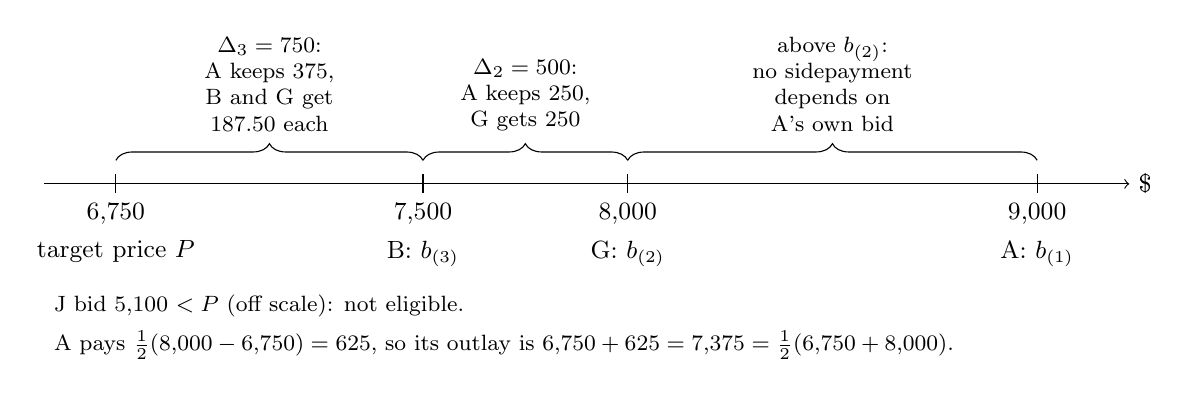
\begin{tikzpicture}[x=1.3cm,y=1cm,font=\small]
\draw[->] (0.3,0) -- (10.9,0) node[right] {\$};
\foreach \x/\v in {1/{6{,}750},4/{7{,}500},6/{8{,}000},10/{9{,}000}}
  {\draw (\x,0.12) -- (\x,-0.12) node[below] {$\v$};}
\node[below] at (1,-0.6) {target price $P$};
\node[below] at (4,-0.6) {B: $b_{(3)}$};
\node[below] at (6,-0.6) {G: $b_{(2)}$};
\node[below] at (10,-0.6) {A: $b_{(1)}$};
\draw[decorate,decoration={brace,amplitude=6pt}] (1,0.3) -- (4,0.3)
  node[midway,above=7pt,align=center,font=\footnotesize]
  {$\Delta_3=750$:\\ A keeps 375,\\ B and G get\\ 187.50 each};
\draw[decorate,decoration={brace,amplitude=6pt}] (4,0.3) -- (6,0.3)
  node[midway,above=7pt,align=center,font=\footnotesize]
  {$\Delta_2=500$:\\ A keeps 250,\\ G gets 250};
\draw[decorate,decoration={brace,amplitude=6pt}] (6,0.3) -- (10,0.3)
  node[midway,above=7pt,align=center,font=\footnotesize]
  {above $b_{(2)}$:\\ no sidepayment\\ depends on\\ A's own bid};
\node[align=left,font=\footnotesize,anchor=west] at (0.3,-1.55) {J bid 5,100 $<P$ (off scale): not eligible.};
\node[align=left,font=\footnotesize,anchor=west] at (0.3,-2.05)
  {A pays $\frac{1}{2}(8{,}000-6{,}750)=625$, so its outlay is $6{,}750+625=7{,}375=\frac{1}{2}(6{,}750+8{,}000)$.};
\end{tikzpicture}
\caption{The incremental sidepayment rule in \cref{ex:13-asker-ko}. Each increment runs from one eligible knockout
bid to the next, between the target price and the second-highest bid. The winner keeps half of it. The losers whose
bids reach its top share the other half equally. Source: drawn from \citet[Example 1]{Asker2010}.}
\label{fig:13-asker-numberline}
\end{figure}

\casehead{An older rule}
Before the late 1980s the ring split each increment equally among all eligible bidders, the winner included.
Under that rule the loser ranked $k$ receives $\sum_{j=k}^{m}\frac{\Delta_j}{j}$. In the example, the \$750
increment would have been shared three ways, giving \$250 each to A, G and B, and the \$500 increment two
ways. G would have received \$500 and B \$250, and A would have paid \$750. Treating bids as true
willingness to pay, the older rule gives each member its imputed Shapley value, a point
\citet{GrahamMarshall1987} make in their analysis of nested knockouts. The \emph{Shapley value} gives each member
its marginal contribution to the coalition's surplus, averaged over all orders in which the members could join. \citet{GrahamMarshallRichard1990} first
studied this class of mechanisms, in which a member's sidepayment rises with its own bid. With two knockout
bidders the old and new rules coincide, since each splits the single increment equally between winner and
loser.

\subsection{The theory of the knockout}\label{sec:13-asker-theory}

Asker adapts the model of \citet{GrahamMarshallRichard1990}. We write $\omega_j$ for member $j$'s participation
probability (Asker writes $\alpha_j$, a symbol this book uses for coefficients). $G$ and $g$ denote the distribution and density
of a rival member's knockout bid. $H_r$ and $h_r$ denote the distribution and density of the highest value among
bidders outside the ring.

\begin{assumption}[Knockout environment]\label{asm:13-asker-ipv}
\leavevmode
\begin{enumerate}[label=(\roman*)]
\item Private values: member $i$'s value $v_i$ is drawn from $F_i$ on $[\underline v_i,\bar v_i]$,
independently across members, and is private information.
\item Members know how many members bid in the knockout but not who they are. Member $j$ participates with known
probability $\omega_j$.
\item Bidders outside the ring bid up to their values in the English target auction, which is weakly dominant
(\cref{sec:14-english-pv}). The highest outside value $r$ has CDF $H_r$ and density $h_r$ and is independent of
members' values. Here $r$ denotes the highest outside value, not a reserve price.
\item Members use increasing, differentiable bid functions $\beta_j$ with inverses $\beta_j^{-1}$. The ring's
agent bids up to the winning knockout bid $b_{(1)}$.
\end{enumerate}
\end{assumption}

Under (iii) and (iv) the ring wins the target auction exactly when $r<b_{(1)}$, and it then pays $P=r$. Every
lot carried a secret reserve price, but Asker finds no evidence that reserves ever bound, so the model omits
them \citep[footnote 12]{Asker2010}.

\casehead{The two-bidder objective}
Consider a member with value $v$ who faces one rival. The rival's bid $y$ has CDF
\[
G(y)=\frac{\sum_{j\neq i}\omega_j F_j\bigl(\beta_j^{-1}(y)\bigr)}{\sum_{j\neq i}\omega_j},
\]
a mixture over the rival's unknown identity, with density $g$. Define the target surplus and sidepayment
integrals
\begin{equation}\label{eq:13-asker-AS}
A(b)\equiv\int_{-\infty}^{b}(v-x)\,h_r(x)\,\dd x,\qquad S(z)\equiv\int_{-\infty}^{z}(z-x)\,h_r(x)\,\dd x .
\end{equation}
If the member bids $b$ and wins the knockout ($y<b$), the ring bids up to $b$. The member gains $v-r$ when
$r<b$, and pays the loser $\frac{1}{2}(y-r)$ when $r<y$. Its expected payoff is $A(b)-\frac{1}{2}S(y)$. If it
loses the knockout ($y>b$), the ring bids up to $y$, and the member receives $\frac{1}{2}(b-r)$ when $r<b$.
Its expected payoff is $\frac{1}{2}S(b)$. Averaging over $y$,
\begin{equation}\label{eq:13-asker-U}
U(b)=\int_{-\infty}^{b}g(y)\Bigl[A(b)-\tfrac{1}{2}S(y)\Bigr]\dd y+\bigl[1-G(b)\bigr]\tfrac{1}{2}S(b).
\end{equation}
This is equation (1) of \citet{Asker2010} after exchanging the order of integration in the sidepayment term.

\casehead{The first-order condition}
We differentiate term by term. By Leibniz's rule, $A'(b)=(v-b)h_r(b)$ and
$S'(z)=(z-z)h_r(z)+\int_{-\infty}^{z}h_r(x)\,\dd x=H_r(z)$. The first term of \eqref{eq:13-asker-U}
splits into $G(b)A(b)$ and $-\frac{1}{2}\int_{-\infty}^{b}g(y)S(y)\,\dd y$. Their derivatives are
\begin{align*}
\frac{\dd}{\dd b}\bigl[G(b)A(b)\bigr]&=g(b)A(b)+G(b)(v-b)h_r(b),\\
\frac{\dd}{\dd b}\Bigl[-\tfrac{1}{2}\textstyle\int_{-\infty}^{b}g(y)S(y)\,\dd y\Bigr]&=-\tfrac{1}{2}g(b)S(b),\\
\frac{\dd}{\dd b}\Bigl[\tfrac{1}{2}\bigl(1-G(b)\bigr)S(b)\Bigr]&=-\tfrac{1}{2}g(b)S(b)+\tfrac{1}{2}\bigl[1-G(b)\bigr]H_r(b).
\end{align*}
Adding the three lines,
\[
U'(b)=g(b)\bigl[A(b)-S(b)\bigr]+G(b)(v-b)h_r(b)+\tfrac{1}{2}\bigl[1-G(b)\bigr]H_r(b).
\]
Since $A(b)-S(b)=\int_{-\infty}^{b}(v-x-b+x)h_r(x)\,\dd x=(v-b)H_r(b)$, we obtain
\begin{equation}\label{eq:13-asker-foc}
U'(b)=(v-b)\Bigl[g(b)H_r(b)+G(b)h_r(b)\Bigr]+\tfrac{1}{2}H_r(b)\bigl[1-G(b)\bigr].
\end{equation}
The first term is the familiar trade-off of a second-price auction. A higher bid wins the knockout more often
(at rate $gH_r$) and wins the target more often after a knockout win (at rate $Gh_r$), each worth $v-b$ at the
margin. The second term is new. When the member loses the knockout and the ring wins below its bid, each extra
dollar of bid brings an extra half dollar of sidepayment.

\begin{lemma}[Asker, Lemma 1]\label{lem:13-asker-lemma1}
At $b=v$, $U'(v)=\frac{1}{2}H_r(v)\bigl[1-G(v)\bigr]\ge0$.
\end{lemma}

\begin{proposition}[Overbidding (Asker, Result 1)]\label{prop:13-overbid}
A member bids strictly above its value whenever $H_r(v)>0$ and $G(v)<1$, and bids its value when $v$ is at the
top of the rival's bid support.
\end{proposition}

\begin{proof}
For $b<v$ both terms of \eqref{eq:13-asker-foc} are nonnegative, so $U$ is nondecreasing on $(-\infty,v]$ and
no bid below $v$ beats $b=v$. At $b=v$, \cref{lem:13-asker-lemma1} gives $U'(v)>0$ when $H_r(v)>0$ and
$G(v)<1$, so some bid above $v$ does strictly better. If $G(v)=1$, then for $b>v$ we have $G(b)=1$ and $g(b)=0$,
so $U'(b)=(v-b)h_r(b)\le0$, and the optimal bid is $v$.
\end{proof}

Asker states the result for any number of knockout bidders. For bids below $v$ the usual dominance argument for
second-price and English auctions applies, and the sidepayment term pushes bids above $v$.

\begin{remark}[Overbidding without sidepayments]\label{rem:13-asker-nosidepay}
Overbidding does not depend on sidepayments \citep[footnote 15]{Asker2010}. Remove them, so the payoff is
$U^0(b)=G(b)A(b)$. Then $U^{0\prime}(v)=g(v)A(v)>0$ whenever the expected target surplus $A(v)$ is positive. A
knockout win removes a rival from the target auction, which has an option value, and a higher bid buys more of
it. In \eqref{eq:13-asker-foc} the sidepayment terms cancel this option value at $b=v$, because $A(v)=S(v)$, and
replace it with the sidepayment motive $\frac{1}{2}H_r(1-G)$.
\end{remark}

\casehead{The inverse bid function}
Setting \eqref{eq:13-asker-foc} to zero and solving for $v$ gives equation (2) of \citet{Asker2010}:
\begin{equation}\label{eq:13-asker-inverse}
v=b-\frac{\frac{1}{2}H_r(b)\bigl[1-G(b)\bigr]}{h_r(b)G(b)+H_r(b)g(b)} .
\end{equation}
The equation maps each observed bid to a unique value, given the distribution of rival bids and the distribution
of the highest outside value. It plays the role that the inversion of \citet{GuerrePerrigneVuong2000} plays for
first-price auctions, $v=b+\frac{G(b)}{(n-1)g(b)}$ (\cref{eq:14-foc-G}, \cref{ch:auction-empirics}). The signs
differ: first-price bidders shade below value, while knockout bidders inflate above it. In both cases
identification requires the inverse bid function to be strictly increasing. Asker also derives three- and
four-bidder analogues (his footnote 13). They involve integrals of $H_r$ against the rival bid distribution,
and the structural analysis uses only two-bidder knockouts.

\begin{corollary}[Inefficiency (Asker, Corollary 1)]\label{cor:13-asker-ineff}
The knockout can lead to an inefficient allocation in the English target auction.
\end{corollary}

Suppose the highest outside value $r$ lies between the top member's value $v_{(1)}$ and that member's knockout
bid $b_{(1)}$. The ring wins and pays $r>v_{(1)}$, although an outside bidder values the lot more. The ring then
harms itself. The seller can gain, because under competition the price would be the second-highest value
overall, which is at most $r$. Outside bidders lose in two ways. They lose the lot they would have won, and when
they do win, the ring's inflated limit $b_{(1)}$ can push their price above the competitive level. Asymmetries
among members add a further inefficiency, because the knockout need not allocate the lot to the member with the
highest value \citep[footnote 16]{Asker2010}.

\begin{lemma}[Asker, Lemma 2]\label{lem:13-asker-lemma2}
The inverse bid function \eqref{eq:13-asker-inverse} can have regions where $\frac{\dd v}{\dd b}<0$.
\end{lemma}

Asker's example sets $H_r$ lognormal with $\mu=-2$ and $\sigma^2=0.08$, and $G$ lognormal with $\mu=-1$ and
$\sigma^2=1$. \Cref{fig:13-asker-vb} confirms the claim: $v(b)$ falls for $b\in[0.161,0.220]$. On that region
some stationary points of the first-order condition are local minima. An estimator could then map observed bids to
values through the wrong branch, which contradicts optimal bidding. Asker therefore maintains that the
population inverse bid function is strictly increasing, and he imposes it through the choice of smoothing
parameters (\cref{sec:13-asker-structural}). With a more dispersed outside value ($\sigma^2=0.5$), the same
$G$ yields a monotone inverse. Both curves lie below the $45^\circ$ line, which is overbidding.

\begin{figure}[htbp]
\centering
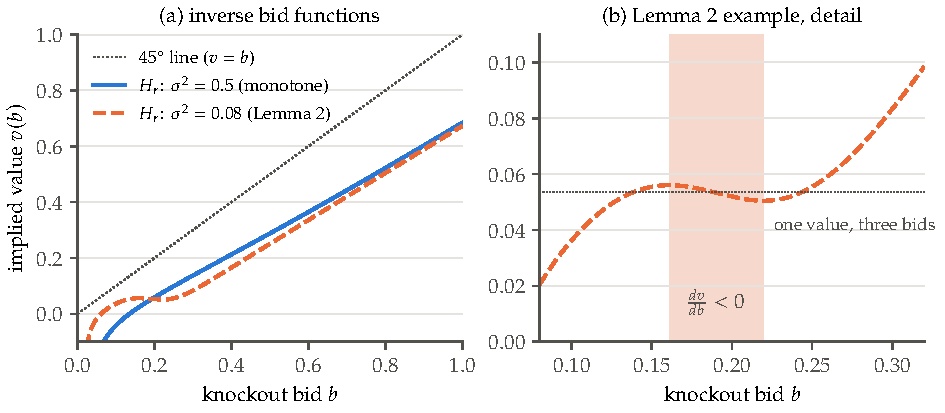
\includegraphics[width=\textwidth]{figures/ch13/asker_vb.pdf}
\caption{The inverse bid function \eqref{eq:13-asker-inverse} with $G$ lognormal ($\mu=-1$, $\sigma^2=1$) and
$H_r$ lognormal with $\mu=-2$. Panel (a): Asker's Lemma 2 example ($\sigma^2=0.08$, dashed) and a monotone case
($\sigma^2=0.5$, solid). Implied values lie below the $45^\circ$ line, so bids exceed values. Panel (b): detail
of the Lemma 2 example. On the shaded region $v(b)$ decreases, so one value is consistent with three bids.
Source: our calculations (\texttt{asker\_inverse\_bid.py}).}
\label{fig:13-asker-vb}
\end{figure}

\subsubsection{Why this mechanism?}

The ring's design looks puzzling. It induces overbidding, misallocation and occasional losses for the ring
itself. Asker's Section II.A explains why simpler designs were unattractive.

\citet{MailathZemsky1991} show that with independent private values drawn from different distributions, a
mechanism exists that achieves efficient collusion at second-price auctions. It balances the budget ex post and
no subcoalition wants to break away. The mechanism depends heavily on the value distributions, however, and
Asker knows of no game form that implements it. With symmetric bidders a simple mechanism is optimal. The ring
holds a first-price sealed-bid knockout, the winner bids in the target, and the winner's knockout bid is split
equally among the losers. With asymmetric bidders that simple design fails. If the ring cannot discriminate in
sidepayments, it may do better to exclude a weak member whose expected contribution to the collusive surplus is
smaller than his share. \citet{McAfeeMcMillan1992} analyze rings at first-price auctions and introduce the
notion of an insincere bidder, an extreme form of weakness. \citet{LopomoMarshallMarx2005} show that when the
knockout follows the target auction and the budget must balance ex post, no scheme at all can implement an
efficient allocation at English auctions. A ring with asymmetric members thus faces a choice. It can exclude its
weak members or accept some inefficiency. The stamp ring kept its weak members.

\begin{remark}[Why tie the target limit to the knockout bid?]\label{rem:13-asker-design}
Consider an alternative in which the knockout winner chooses its own limit in the target auction, with
sidepayments computed as before. Suppose two members bid and the bids become known. Let the winner's value be
$v_1$ and the loser's bid $k_2$. If $k_2<v_1$, the standard English auction argument gives a limit of $v_1$. If
$k_2>v_1$, the winner chooses a limit $\bar b\le k_2$ to maximize
\[
\int_{-\infty}^{\bar b}(v_1-x)\,h_r(x)\,\dd x-\frac{1}{2}\int_{-\infty}^{\bar b}(k_2-x)\,h_r(x)\,\dd x .
\]
The first-order condition is $(v_1-\bar b)h_r(\bar b)-\frac{1}{2}(k_2-\bar b)h_r(\bar b)=0$, so
\[
v_1-\bar b=\tfrac{1}{2}(k_2-\bar b)\quad\Longrightarrow\quad\bar b=2v_1-k_2<v_1 .
\]
The winner would underbid, to avoid winning lots whose sidepayment exceeds its profit \citep[p.~734 and
footnote 19]{Asker2010}. Underbidding would leave profitable lots unbought and invite members to defect and bid
secretly against the ring. It would also attract outside bidders. Tying the limit to the knockout bid makes the
ring aggressive instead. No member wants to be outside a ring that overbids, and outsiders are deterred from
entering. On this account the design traded some allocative efficiency for stability.
\end{remark}

\subsection{Data and descriptive evidence}\label{sec:13-asker-data}

The data cover the knockouts before 11 target sales between June 5, 1996 and June 26, 1997. A sale is a
collection of lot auctions that often runs over several days. The New York Attorney General's office collected
the records during its investigation. They were transcribed from faxes and written records kept by one member,
who was known in the ring for worrying about not being paid what he was owed. For each lot the data give the
date, auction house, lot number, target price, all sidepayments, and the identities and bids of the knockout
bidders. Fewer than 3 percent of observations are incomplete, for reasons such as faxes faded by sunlight. The
records are matched to auction catalogs, which report estimated minimum and maximum values or a book value,
condition grades, origin and number of stamps. The main shortcoming is that the number of bidders in the target
auction is unknown, and only the winning target price is recorded \citep[pp.~734--735]{Asker2010}.

The analysis excludes the Harmer-Schau sale (189 lots, 87 percent won by the ring), where the ring used an
informal arrangement and the target price almost always equaled the second-highest knockout bid. In the
remaining 1,781 lots the ring won 58 percent of the lots on which it was active, or 66 percent by estimated
value. The lots it won raised \$6,377,284, against \$10,034,754 across all lots on which it was active. The
pooled mean knockout bid was \$2,142 and the pooled mean winning target bid \$2,042 \citep[Table
1]{Asker2010}.

\Cref{tab:13-asker-t2} organizes the lots by the number of members in the knockout. A single member bid on
623 lots, and eight members bid on 26. The ring's win rate rises steeply with participation, from 19 percent to
96 percent. Either outside participation grew more slowly than ring participation, or overbidding grew with the
number of members, or both. Mean winning target bids rise weakly with participation and are roughly flat between
three and six bidders.

\begin{table}[htbp]
\centering
\caption{Bidding by number of bidders in the knockout}
\label{tab:13-asker-t2}
\begin{threeparttable}
\begin{tabular}{@{}crrrrrr@{}}
\toprule
Number of & \multicolumn{2}{c}{\makecell{Target auction\\(winning bid)}} &
\multicolumn{2}{c}{\makecell{Knockout\\(median bid)}} & \% of lots & Total \\
\cmidrule(lr){2-3}\cmidrule(lr){4-5}
bidders & Mean & SD & Mean & SD & won by ring & lots \\
\midrule
1 & 733 & 1,262 & 616 & 1,134 & 19 & 623 \\
2 & 1,314 & 2,016 & 1,066 & 2,048 & 36 & 367 \\
3 & 2,014 & 3,246 & 1,750 & 3,029 & 48 & 260 \\
4 & 2,217 & 3,492 & 2,293 & 4,082 & 69 & 196 \\
5 & 2,249 & 3,419 & 2,092 & 3,322 & 68 & 144 \\
6 & 2,098 & 2,628 & 2,163 & 3,014 & 74 & 91 \\
7 & 2,979 & 3,425 & 3,655 & 4,116 & 86 & 74 \\
8 & 4,790 & 4,904 & 6,233 & 7,726 & 96 & 26 \\
\bottomrule
\end{tabular}
\begin{tablenotes}\footnotesize
\item Notes: Amounts in dollars. Excludes the Harmer-Schau sale. The lot counts sum to 1,781. Weighting the win
rates by lots gives about 43 percent, below the 58 percent of Asker's Table 1, so the two figures are computed
on different bases. Source: \citet[Table 2]{Asker2010}.
\end{tablenotes}
\end{threeparttable}
\end{table}

\casehead{Participation and win rates}
Asker's Table 3 regresses the number of members in each knockout on lot characteristics by OLS. A second
column uses a transformed logit, whose dependent variable is the log share of members participating minus the
log share not participating. In the logit, participation rises with the spread of the catalog estimate,
$E_{\max}-E_{\min}$ in thousands of dollars (coefficient 0.196, standard error 0.103), much more than with its
midpoint (0.031, standard error 0.024). It also rises with the spread of condition grades (0.198, standard error
0.022) and falls when no grade is given ($-0.492$, standard error 0.074). Both regressions use 1,781 lots, with
an $R^2$ of 0.261 for OLS and 0.255 for the logit. Participation is always incomplete: at most 8 of the 11
members ever bid on a lot. Since entering a very low knockout bid costs little and can earn a sidepayment, Asker suggests a dynamic
enforcement rule or a small participation cost as explanations \citep[pp.~737--738]{Asker2010}.

Table 4 of \citet{Asker2010} reports a logit of a ring win on the same covariates. The number of members raises
the win probability, with a coefficient of 0.854 (standard error 0.127) and a marginal effect of 0.208 per
member. The effect diminishes, with a coefficient of $-0.046$ (0.017) on the square. Higher average grades raise
the win probability (0.313, standard error 0.069). The estimated value and its spread have no significant effect
once these are controlled for. Auction house dummies remain significant, perhaps because outside competition
differed across houses.

\casehead{Weak members}
\Cref{tab:13-asker-t5} reports knockout outcomes by member. Members D, G and H rarely submit the high bid: 14, 11
and 14 percent of the knockouts they enter, and 10, 10 and 4 percent when at least two members bid. Yet they
receive sidepayments at least as often as the others (20, 34 and 34 percent) and almost never pay them (3, 5
and 0 percent). In an independent private values model, a member's strength comes from its value distribution.
A weak member's distribution places more mass on low values. Asker notes that distributions with a similar mean
but a much lower variance fit the pattern. Such members lose more often, but their losing bids sit close to the
winning bid and so earn sidepayments \citep[footnote 30]{Asker2010}. Member D was explicit in his deposition.
His objective, he said, was to ``make money from these people'' rather than to buy the stamps
\citep[p.~738]{Asker2010}.

\begin{table}[htbp]
\centering
\caption{Knockout outcomes, by ring member}
\label{tab:13-asker-t5}
\begin{threeparttable}
\begin{tabular}{@{}lrrrrrr@{}}
\toprule
 & \multicolumn{2}{c}{All knockouts ($n\ge1$)} & \multicolumn{4}{c}{Knockouts with at least two members ($n\ge2$)} \\
\cmidrule(lr){2-3}\cmidrule(l){4-7}
Member & \% high bid & Knockouts & \% high bid & \% receives & \% pays & Knockouts \\
\midrule
A & 40 & 675 & 33 & 22 & 12 & 607 \\
B & 57 & 196 & 52 & 21 & 16 & 175 \\
C & 34 & 449 & 20 & 23 & 5 & 368 \\
D & 14 & 715 & 10 & 20 & 3 & 686 \\
E & 39 & 353 & 38 & 24 & 21 & 348 \\
F & 31 & 120 & 28 & 28 & 4 & 116 \\
G & 11 & 186 & 10 & 34 & 5 & 184 \\
H & 14 & 56 & 4 & 34 & 0 & 50 \\
I & 44 & 210 & 44 & 17 & 20 & 209 \\
J & 45 & 878 & 30 & 22 & 9 & 686 \\
K & 42 & 1,075 & 28 & 21 & 9 & 861 \\
\bottomrule
\end{tabular}
\begin{tablenotes}\footnotesize
\item Notes: ``\% high bid'' is the share of a member's knockouts in which it submitted the highest bid.
``\% receives'' and ``\% pays'' are the shares in which it received or paid sidepayments. Source:
\citet[Table 5]{Asker2010}.
\end{tablenotes}
\end{threeparttable}
\end{table}

\Cref{fig:13-asker-f1} shows net sidepayments by member. Over all auctions, E was the largest net payer, with
\$74,418 paid into the ring. D and G were the largest net recipients, with \$22,251 and \$21,574, although G
took part in only 186 knockouts against D's 715. Excluding the 25 lots with target prices above \$10,000 reduces
E's role. E was active in 18 of them and paid \$38,000 net on them. Its largest single payment was \$15,500, on
a lot acquired for \$26,000. The ability of D and H to extract sidepayments is unchanged by the exclusion
\citep[p.~740 and footnote 28]{Asker2010}.

\begin{figure}[htbp]
\centering
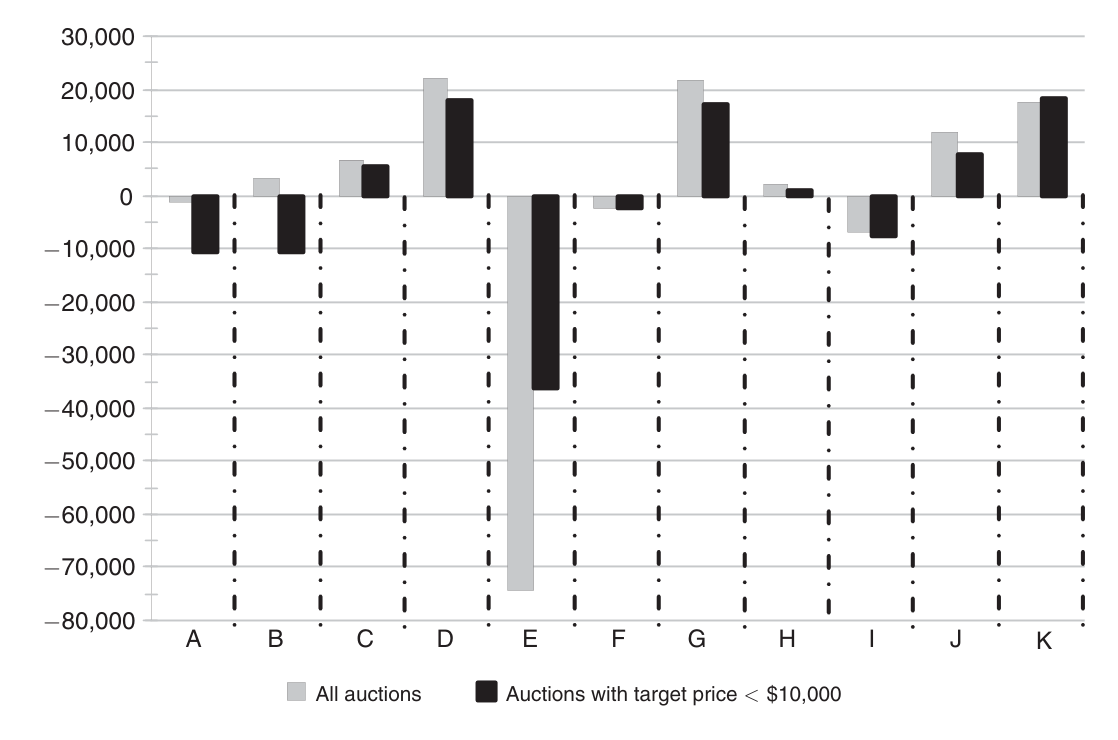
\includegraphics[width=0.82\textwidth]{figures/ch13/asker2010_fig1.png}
\caption{Net sidepayments from the ring, by member, in dollars. Positive values are net receipts. Grey bars
cover all auctions, and black bars cover auctions with target prices below \$10,000. Source: \citet{Asker2010},
Figure 1.}
\label{fig:13-asker-f1}
\end{figure}

\casehead{Naive damages}
A naive measure of the seller's loss treats knockout bids as true values. In an English auction without the
ring, the price would be the second-highest value among all bidders. When the ring wins, the target price is the
highest outside value. The naive damage on a lot the ring won is therefore
\begin{equation}\label{eq:13-asker-naive}
\text{naive damage}_k=\max\bigl\{b_{(2),k}-P_k,\,0\bigr\}.
\end{equation}
\Cref{tab:13-asker-t6} reports the measure for the 1,158 lots with at least two members in the knockout, which
are the 1,781 lots minus the 623 single-member lots. Total naive damages are \$514,900. The mean of \$445 per lot
divides by all 1,158 lots, including the 509 the ring did not win. Naive damages rise with the target price,
reaching \$3,820 per lot above \$10,000, and with the number of members, reaching \$3,796 per lot in
eight-member knockouts. By auction house, Matthew Bennett, a stamp specialist, bears the largest total, \$283,200
\citep[Table 6]{Asker2010}. The measure overstates true damages, because \cref{prop:13-overbid} implies that
$b_{(2)}$ exceeds the second-highest member's value. Measuring true damages requires the structural model.

\begin{table}[htbp]
\centering
\caption{Naive damages in target auctions with two or more ring members active in the knockout}
\label{tab:13-asker-t6}
\footnotesize
\setlength{\tabcolsep}{3.5pt}
\begin{threeparttable}
\begin{tabular}{@{}lrrrrrrrrr@{}}
\toprule
\multicolumn{10}{@{}l}{\textit{By final price in target auction (\$)}} \\
 & 0--500 & 501-- & 1,001-- & 2,001-- & 3,001-- & 5,001-- & 7,001-- & 10,000+ & Aggregate \\
 & & 1,000 & 2,000 & 3,000 & 5,000 & 7,000 & 10,000 & & \\
\midrule
Mean target price & 314 & 745 & 1,483 & 2,527 & 3,929 & 5,940 & 8,514 & 17,180 & 1,986 \\
Mean highest knockout bid & 471 & 1,066 & 1,996 & 3,187 & 5,918 & 8,041 & 10,428 & 23,840 & 2,718 \\
Mean total sidepayments & 42 & 92 & 154 & 245 & 622 & 697 & 526 & 1,910 & 222 \\
Total naive damages & 28,390 & 53,460 & 68,000 & 51,950 & 113,150 & 65,500 & 38,950 & 95,500 & 514,900 \\
Mean naive damages & 83 & 184 & 308 & 490 & 1,243 & 1,394 & 1,053 & 3,820 & 445 \\
Lots won by ring & 203 & 162 & 112 & 50 & 55 & 29 & 23 & 15 & 649 \\
Total lots & 341 & 290 & 221 & 106 & 91 & 47 & 37 & 25 & 1,158 \\
\midrule
\multicolumn{10}{@{}l}{\textit{By number of ring members in knockout}} \\
 & 2 & 3 & 4 & 5 & 6 & 7 & 8 & & Aggregate \\
\midrule
Mean target price & 1,314 & 2,014 & 2,217 & 2,249 & 2,098 & 2,979 & 4,790 & & 1,986 \\
Mean highest knockout bid & 1,281 & 2,327 & 3,197 & 3,282 & 3,301 & 5,750 & 9,496 & & 2,718 \\
Mean total sidepayments & 12 & 96 & 249 & 211 & 365 & 895 & 1,898 & & 222 \\
Total naive damages & 8,920 & 50,095 & 97,540 & 60,760 & 66,415 & 132,470 & 98,700 & & 514,900 \\
Mean naive damages & 24 & 193 & 498 & 422 & 730 & 1,790 & 3,796 & & 445 \\
Lots won by ring & 133 & 126 & 136 & 98 & 67 & 64 & 25 & & 649 \\
Total lots & 367 & 260 & 196 & 144 & 91 & 74 & 26 & & 1,158 \\
\bottomrule
\end{tabular}
\begin{tablenotes}\footnotesize
\item Notes: Amounts in dollars. Naive damages are the second-highest knockout bid minus the target price on lots
the ring won. Mean naive damages divide total naive damages by total lots (for example,
$\frac{514{,}900}{1{,}158}=445$). The source also reports a panel by auction house. Source: \citet[Table
6]{Asker2010}.
\end{tablenotes}
\end{threeparttable}
\end{table}

\subsection{Structural estimation}\label{sec:13-asker-structural}

The structural model recovers the distributions of members' values and of the highest outside value from bids.
With these distributions, damages, efficiency losses and the ring's returns can be simulated. The estimator
adapts \citet{GuerrePerrigneVuong2000} and is closest to Krasnokutskaya's treatment of unobserved heterogeneity
\citep{Krasnokutskaya2011}, which Asker cites in its 2004 working-paper form.

\casehead{Primitives}
Member $i$'s value for lot $k$ is
\begin{equation}\label{eq:13-asker-value}
u_{ik}=\Gamma(x_k)\,v_{ik}\,\kappa_k,\qquad\Gamma(x_k)=e^{x_k\gamma}.
\end{equation}
The row vector $x_k$ holds the catalog's estimated minimum and maximum values and a catalog value if one is
provided. It also holds the minimum and maximum condition grades, a dummy for lots of exclusively US stamps,
and a dummy for lots without value estimates. The factor $\kappa_k$ is lot heterogeneity that bidders observe and the
econometrician does not, such as information from inspecting the stamps. The private component $v_{ik}$ reflects
a dealer's clients, its cost of capital and its private information about the market. In the basic model
$\kappa_k=1$. The multiplicative form lets both the mean and the variance of values move with observed
characteristics. Only two-bidder knockouts are used. Members D, G and H form a weak type and the others a strong
type, with a common value distribution within each type. Each bidder knows that it faces one rival of unknown
type, and the empirical participation frequencies serve as the probabilities $\omega_j$.

\begin{lemma}[Homogeneity (Asker, Lemma 3)]\label{lem:13-asker-homog}
In a two-bidder knockout, suppose $b$ is an optimal bid at value $v$ when all values are as given. If every
member's value and the highest outside value are multiplied by $\Gamma>0$, there is an equilibrium in which the
optimal bid at value $\Gamma v$ is $\Gamma b$.
\end{lemma}

\begin{proof}
We mark objects of the scaled game with a superscript $\Gamma$. Let every member use
$\beta_j^{\Gamma}(u)=\Gamma\beta_j(\frac{u}{\Gamma})$ in the scaled game. The rival's bid then has CDF
$G^{\Gamma}(y)=G(\frac{y}{\Gamma})$ and density $g^{\Gamma}(y)=\frac{1}{\Gamma}g(\frac{y}{\Gamma})$. The highest
outside value has $H_r^{\Gamma}(x)=H_r(\frac{x}{\Gamma})$ and $h_r^{\Gamma}(x)=\frac{1}{\Gamma}h_r(\frac{x}{\Gamma})$.
Substitute $x=\Gamma\tilde x$ and $y=\Gamma\tilde y$ in each integral of \eqref{eq:13-asker-U}. For example,
\[
\int_{-\infty}^{\Gamma\tilde b}(\Gamma v-x)\,h_r^{\Gamma}(x)\,\dd x
=\int_{-\infty}^{\tilde b}\Gamma(v-\tilde x)\,\frac{1}{\Gamma}h_r(\tilde x)\,\Gamma\,\dd\tilde x
=\Gamma\int_{-\infty}^{\tilde b}(v-\tilde x)\,h_r(\tilde x)\,\dd\tilde x ,
\]
and $g^{\Gamma}(y)\,\dd y=g(\tilde y)\,\dd\tilde y$. Every term scales in the same way. The scaled objective
$U^{\Gamma}$ therefore satisfies $U^{\Gamma}(\Gamma\tilde b;\Gamma v)=\Gamma\,U(\tilde b;v)$ for every bid
$\tilde b$. A positive multiple of an objective has the same maximizers, so $\tilde b$ is optimal at $v$ if and
only if $\Gamma\tilde b$ is optimal at $\Gamma v$. The argument applies to each member, so the scaled profile is
an equilibrium.
\end{proof}

Asker proves the lemma from the first-order conditions in his appendix. He reports that it does not hold for
knockouts with three or more bidders, which is why only two-bidder knockouts enter the structural analysis. For
three-bidder knockouts he estimated an additive version, whose results he judged explicable only by strong
misspecification \citep[footnote 34]{Asker2010}. Applying the lemma with $\Gamma=\Gamma(x_k)\kappa_k$ gives
log bids of the form
\begin{equation}\label{eq:13-asker-logbid}
\ln b_{ik}=x_k\gamma+\ln\kappa_k+\ln\beta(v_{ik}),
\end{equation}
where $\beta$ is the bid function at normalized values. By the dominant strategy argument the same scaling holds
for outside bidders, so the target price on a lot the ring wins is $\ln P_k=x_k\gamma+\ln\kappa_k+\ln r_k$.

\casehead{Step 1: observed heterogeneity}
Following \citet{HaileHongShum2003}, Asker runs the first-stage regression
\begin{equation}\label{eq:13-asker-firststage}
\ln b_{ik}=x_k\gamma+a_i+e_{ik},
\end{equation}
which is his equation (3). The sample pools the knockout bids and the target prices, so that $i$ ranges over the
members and the target. The terms $a_i$ are dummies for each member and for the target price, and $e_{ik}$ is an
error. Pooling preserves the relative ordering of bids within a lot. The normalized bids are
$\ln\hat b_{ik}=\ln b_{ik}-x_k\hat\gamma$. The first stage removes much of the heterogeneity across lots. The
standard deviation of lot-mean bids falls from 1,367 before the normalization to 370 after it
\citep[footnote 45]{Asker2010}.

\casehead{Step 2: unobserved heterogeneity}
After normalization, the two bids on a lot share the common component $\ln\kappa_k$:
\begin{equation}\label{eq:13-asker-pairs}
\ln\hat b_{1k}=\ln\kappa_k+\ln\beta(v_{1k}),\qquad\ln\hat b_{2k}=\ln\kappa_k+\ln\beta(v_{2k}).
\end{equation}
This is a measurement-error structure with two indicators of a common factor. \citet{LiVuong1998} showed how to
estimate it nonparametrically, building on an identification result of \citet{Kotlarski1966}. The same result
underlies Krasnokutskaya's estimator (\cref{ch:auction-empirics}).

We state the result in the notation of \cref{lem:B-kotlarski}, which proves it. There $\psi_X(t)=\E[e^{\mathrm{i}tX}]$
is the \emph{characteristic function} of a random variable $X$, and $\psi_Q$ is the joint characteristic function of a
pair $(Q_1,Q_2)$.

\begin{theorem}[Kotlarski 1966]\label{thm:13-kotlarski}
Let $Y_1$, $Y_2$ and $Y_3$ be mutually independent with nonvanishing characteristic functions, with
$\E|Y_1|<\infty$, $\E|Y_3|<\infty$ and $\E[Y_1]=0$. Then the joint distribution of $Q_1=Y_1+Y_3$ and
$Q_2=Y_2+Y_3$ determines the distributions of $Y_1$, $Y_2$ and $Y_3$ through \eqref{eq:B-kotlarski}
(\cref{lem:B-kotlarski}).
\end{theorem}

Each assumption has a role. Independence delivers the factorization on which the proof rests,
\begin{equation*}
\psi_Q(t_1,t_2)=\psi_{Y_1}(t_1)\,\psi_{Y_2}(t_2)\,\psi_{Y_3}(t_1+t_2).
\end{equation*}
The nonvanishing
condition allows the divisions and the logarithm in \eqref{eq:B-kotlarski}. The zero mean of $Y_1$ is a location
normalization. Without it, a constant could be moved freely between $Y_3$ and the idiosyncratic components.

In Asker's application $Q_j=\ln\hat b_{jk}$, $Y_3=\ln\kappa_k$ and $Y_j=\ln\beta(v_{jk})$ for $j=1,2$, where
bidder 1 is always a strong member \citep[footnote 35]{Asker2010}. When both bidders are strong, $Y_1$ and $Y_2$
share a distribution. The estimator replaces $\psi_Q$ by the empirical characteristic function over the $K$
lots,
\begin{equation}\label{eq:13-asker-ecf}
\hat\psi_Q(z_1,z_2)=\frac{1}{K}\sum_{k=1}^{K}\exp\bigl(\mathrm{i}z_1\ln\hat b_{1k}+\mathrm{i}z_2\ln\hat b_{2k}\bigr),
\end{equation}
plugs it into \eqref{eq:B-kotlarski}, and recovers each density by a damped inverse Fourier transform (Asker's
equation (5)):
\begin{equation}\label{eq:13-asker-fourier}
\hat g_X(x)=\frac{1}{2\pi}\int_{-T_n}^{T_n}d(t)\,e^{-\mathrm{i}tx}\,\hat\psi_X(t)\,\dd t,\qquad
X\in\bigl\{\ln\kappa,\ln\beta(v_1),\ln\beta(v_2)\bigr\}.
\end{equation}
Here $d(t)$ is a damping function and $T_n$ a smoothing parameter.

\begin{assumption}[Asker's Assumption U]\label{asm:13-asker-U}
(a) The normalized bids satisfy \eqref{eq:13-asker-pairs} with $\E[\ln\beta(v_1)]=0$. (b) The components
$\ln\kappa$, $\ln\beta(v_1)$ and $\ln\beta(v_2)$ are mutually independent. (c) Their characteristic functions
never vanish. Regularity conditions on smoothness and integrability follow \citet{LiVuong1998}.
\end{assumption}

Part (b) rests on the independence of private information across bidders. Part (a) is the normalization of
\cref{thm:13-kotlarski}. Within-lot variation identifies the private components only up to location, so their
position is fixed by the mean of the strong component. A practical consequence follows. Unlike the estimator of
\citet{GuerrePerrigneVuong2000}, this approach identifies only distributions. It cannot recover the value behind
any particular bid.

The target price adds a third measurement. On lots the ring wins, $\ln r_k^*\equiv\ln\hat P_k=\ln\kappa_k+\ln r_k$.
Asker applies the procedure to both pairs $\{\ln\beta(v_2),\ln\beta(v_1)\}$ and $\{\ln r^*,\ln\beta(v_1)\}$, setting
aside for the moment that target prices are observed only when the ring wins. Each pair yields an estimate of
$\psi_{\ln\kappa}$, and the two are averaged with weights equal to the number of observations, as
\citet{LiVuong1998} suggest. Variation across lots identifies the distribution of $\ln\kappa$, and variation within
lots identifies the distributions of the private components \citep[pp.~745--746]{Asker2010}.

\casehead{Step 3: selection in the target price}
The target price reveals the highest outside value only when the ring wins, that is, when $r$ falls below the
highest knockout bid $b_{\max}$. Let $G_m$ and $g_m$ be the distribution and density of $b_{\max}$, and let
$\tilde h_r$ be the density of $r$ among lots the ring wins.

\begin{proposition}[Selection correction]\label{prop:13-asker-selection}
Suppose $r$ is independent of $b_{\max}$ and the support of $r$ lies within that of $b_{\max}$. Then
\begin{equation}\label{eq:13-asker-selection}
h_r(r)=\mathcal{A}\,\frac{\tilde h_r(r)}{1-G_m(r)},\qquad
H_r(r)=\mathcal{A}\int_{-\infty}^{r}\frac{\tilde h_r(x)}{1-G_m(x)}\,\dd x,\qquad
\mathcal{A}=\left[\int_{-\infty}^{\infty}\frac{\tilde h_r(x)}{1-G_m(x)}\,\dd x\right]^{-1}.
\end{equation}
\end{proposition}

\begin{proof}
By independence, the selected distribution is
\[
\tilde H_r(\rho)=\Pr(r\le\rho\mid r<b_{\max})=\frac{\int_{-\infty}^{\rho}h_r(x)\Pr(b_{\max}>x)\,\dd x}{\Pr(r<b_{\max})}
=\frac{1}{\mathcal{A}}\int_{-\infty}^{\rho}h_r(x)\bigl[1-G_m(x)\bigr]\dd x ,
\]
with $\mathcal{A}=\int h_r(x)[1-G_m(x)]\,\dd x=\Pr(r<b_{\max})$. Differentiating gives
$\mathcal{A}\,\tilde h_r(r)=h_r(r)[1-G_m(r)]$. The support condition ensures $1-G_m(r)>0$ wherever $h_r(r)>0$, so we
can divide. This gives the first formula. Integrating gives the second. Requiring $H_r(\infty)=1$ gives the third.
\end{proof}

Both $\tilde h_r$ and $G_m$ can be estimated from the data. The support condition says that the highest knockout
bid can reach at least as high as the highest outside value. Given overbidding, Asker judges it unrestrictive
\citep[p.~747]{Asker2010}.

\casehead{Step 4: from bids to values}
The densities of $\beta(v_1)$, $\beta(v_2)$ and $r$ are estimated with the triweight kernel
$K(u)=\frac{35}{32}(1-u^2)^3\indic(|u|<1)$, and their distribution functions by empirical distribution functions.
Combined with the participation frequencies, these estimates form $G$, $g$, $H_r$ and $h_r$. Equation \eqref{eq:13-asker-inverse} then maps bids to
values, separately for the strong and weak types.

\casehead{Step 5: simulated auctions}
Asker draws from the estimated distributions of $\kappa$, $\beta(v_1)$, $\beta(v_2)$ and $r$, converts bids into
values with Step 4, and recombines the pieces into 100,000 pseudo-auctions. Observed heterogeneity is added by
drawing from the empirical joint distribution of $x_k$. The two percent of draws with bids outside the observed bid
range are dropped. Confidence intervals come from a bootstrap that resamples auctions, with 5,000 replications.

\casehead{Practical choices}
The damping function is $d(t)=\max\bigl[1-\frac{|t|}{\sqrt2\,T_n},0\bigr]$, following \citet{DiggleHall1993}. The
smoothing parameter $T_n$ is chosen in two stages. A linear extrapolation rule of Diggle and Hall gives a range.
Within it Asker minimizes
\[
\left(\frac{\widehat{ND}-ND}{ND}\right)^2+\left(\frac{\widehat{PW}-PW}{PW}\right)^2+P\,\indic\{\text{nonmonotonic}\},
\]
where $ND$ is mean naive damages, $PW$ the probability that the ring wins, hats denote simulated values, and the
last term penalizes nonmonotone inverse bid functions (\cref{lem:13-asker-lemma2}). The common component is well
identified and insensitive to $T_n$, so $T_n=50$ for $\ln\kappa$. The search gives $T_n=12.0$, $3.0$ and $8.3$ for
the strong component, the weak component and $\ln r$. Deconvolution estimates are imprecise in the tails, which
makes the ratio in \eqref{eq:13-asker-selection} unstable, so supports are trimmed using the largest within-lot
differences between bids. Kernel bandwidths follow the rule of thumb $h=1.06\,\hat\sigma n^{-\frac{1}{6}}$, and
smoothed distribution functions use $h=1.06\,\hat\sigma n^{-\frac{1}{5}}$. One outlier is dropped. Its knockout
bids were \$42,500 and \$18,000 and its target price \$18,000, while the next highest bid in any two-bidder
knockout was \$13,500 \citep[pp.~748--749]{Asker2010}.

\casehead{Identification and counterfactuals}
The argument has three layers. Variation across lots identifies the distribution of the common component.
Variation within lots identifies the private components. The first-order condition \eqref{eq:13-asker-inverse}
maps the bid distribution into the value distribution, provided the population inverse is increasing. The
argument also needs a single equilibrium in the data and knowledge of the number of knockout bidders. Damages
compare the ring's outcome with a competitive English auction in which all bidders bid their values. When the ring
wins, it pays $P_r=r$. The competitive price $P_c$ is the second-highest value among all bidders, which depends on
the second-highest outside value $r_{(2)}$. The data do not identify it, so Asker brackets it with two assumptions.
\begin{itemize}
\item U.B. (upper bound on damages): $r_{(2)}=r$. Then $P_c\ge r=P_r$, so sellers never gain, and the competitive
price takes its highest model-consistent value.
\item L.B. (lower bound on damages): $r_{(2)}=\min\{r,v_{(1)}\}$, with $v_{(1)}$ the highest member value. If the
ring won with $r>v_{(1)}$, a misallocation, then $P_c=v_{(1)}<P_r$ and the seller gains. Otherwise $P_c$ is as
under U.B.
\end{itemize}
Under both assumptions the seller loses exactly when the second-highest member value exceeds $r$. The share of
ring wins in which sellers gain under L.B. therefore equals the share of misallocations.

\subsection{Results}\label{sec:13-asker-results}

\Cref{fig:13-asker-f2} shows the estimated bid function of a strong member, evaluated at a common component of
520 and a 70 percent chance of facing another strong member. Bids lie above the $45^\circ$ line throughout.
Overbidding is roughly constant at low values and declines once values exceed about \$750, as the chance of
winning the target rises. A member with a value of \$800 would win the target with probability 0.44 if it bid
its value. It bids \$877, which raises that probability to 0.446. The bid function of a weak member is very
similar \citep[p.~750]{Asker2010}.

\begin{figure}[htbp]
\centering
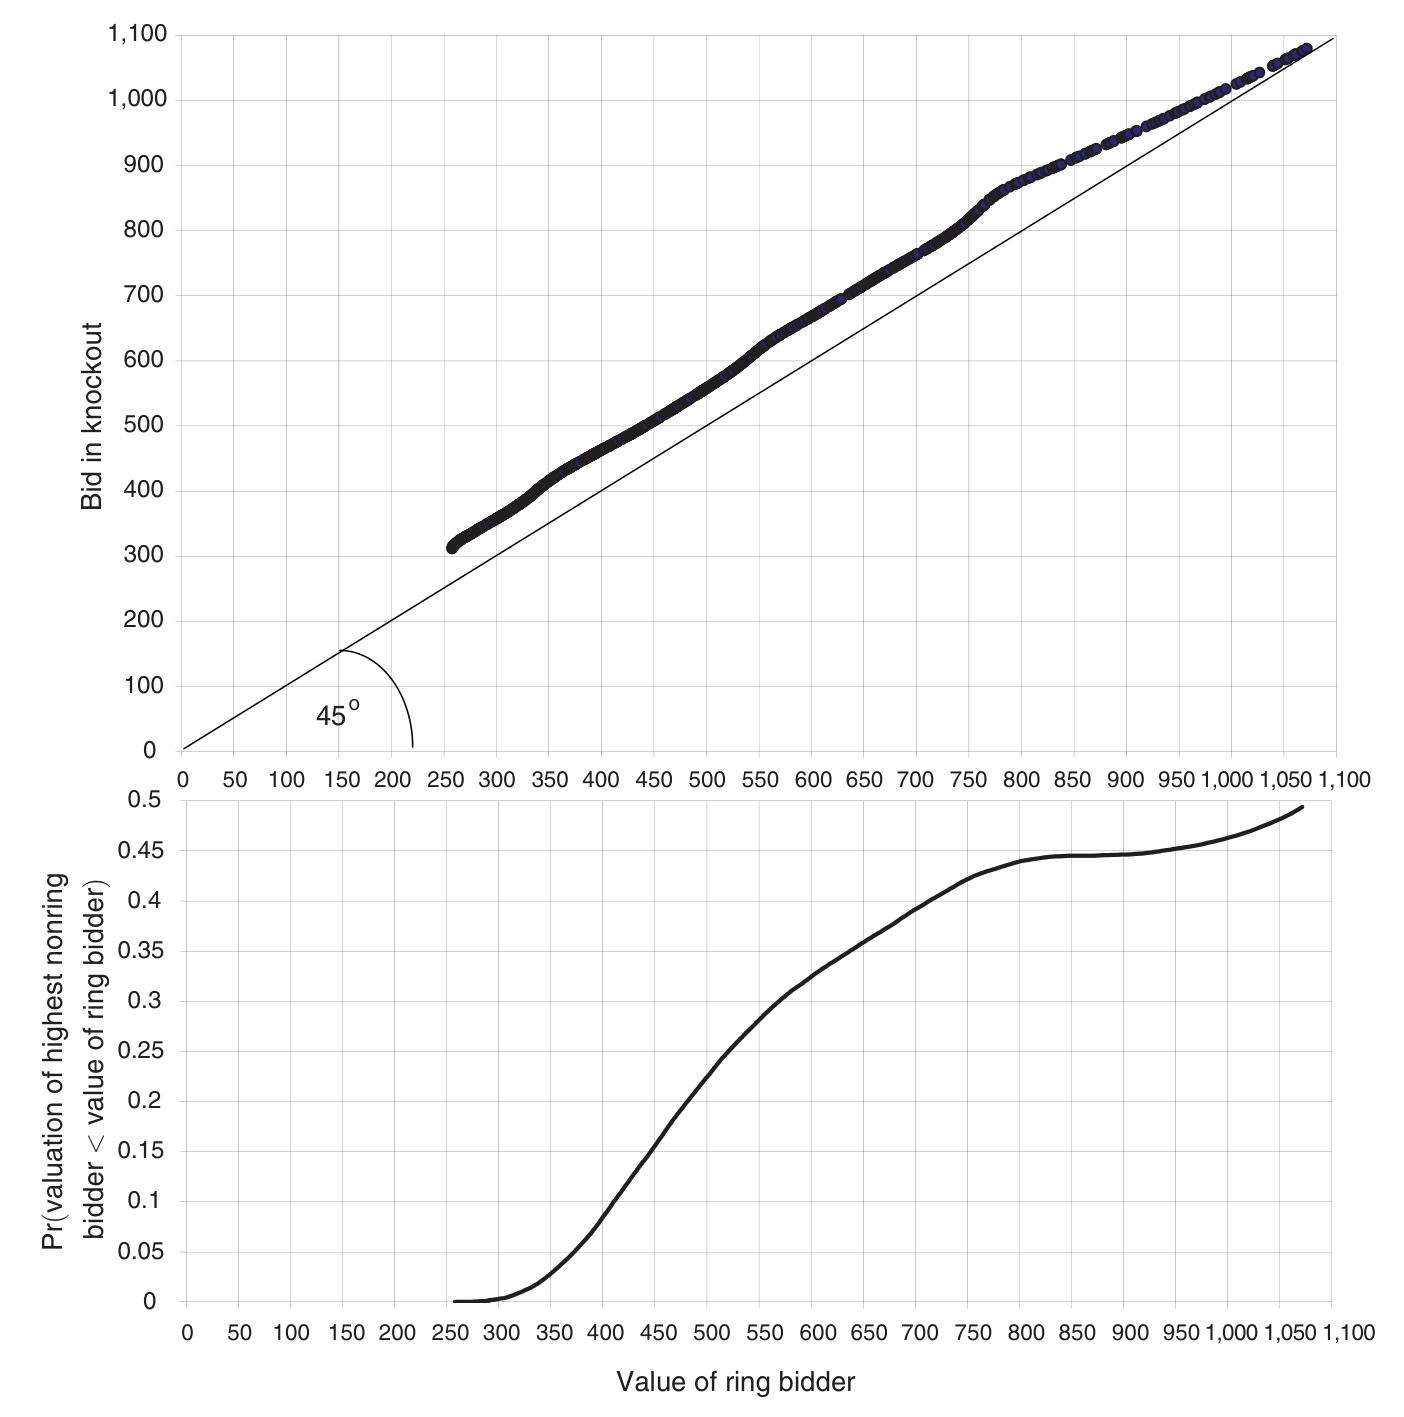
\includegraphics[width=0.86\textwidth]{figures/ch13/asker2010_fig2.png}
\caption{Estimated knockout bid function of a strong member in the model with unobserved lot heterogeneity
(top), and the probability that the highest outside value lies below the member's value (bottom). The bid function
is constructed with a common component of 520 and a 70 percent chance of facing another strong member. Source:
\citet{Asker2010}, Figure 2.}
\label{fig:13-asker-f2}
\end{figure}

\casehead{Damages to sellers}
\Cref{tab:13-asker-t7} reproduces Asker's Table 7. In the data, mean naive damages on lots the ring won are \$67
among two-bidder knockouts. The model with unobserved heterogeneity predicts \$74, and the model without it
predicts \$150. Without a common component, simulated bids vary too much within lots. Both models match the
ring's win rate well, at 0.34 and 0.37 against 0.36 in the data, although the intervals are wide. With
unobserved heterogeneity, mean true damages per ring win are \$36.99 under U.B. and \$26.50 under L.B. These are
about half and about a third of the model's naive damages of \$74.21. The 90 percent confidence intervals for the
ratio of true to naive damages are $[0.38,0.69]$ under U.B. and $[0.25,0.63]$ under L.B. \citep[footnote
47]{Asker2010}. Ignoring unobserved heterogeneity raises true damages to \$105.74 and \$99.15.

\begin{table}[htbp]
\centering
\caption{Damages to the seller}
\label{tab:13-asker-t7}
\footnotesize
\setlength{\tabcolsep}{4pt}
\begin{threeparttable}
\begin{tabular}{@{}llrrrrrr@{}}
\toprule
 & & \multicolumn{3}{c}{\makecell{With unobserved\\heterogeneity}} & \multicolumn{3}{c}{\makecell{No unobserved\\heterogeneity}} \\
\cmidrule(lr){3-5}\cmidrule(l){6-8}
 & & & \multicolumn{2}{c}{90\% interval} & & \multicolumn{2}{c}{90\% interval} \\
\cmidrule(lr){4-5}\cmidrule(l){7-8}
 & Assumption & Point & Lower & Upper & Point & Lower & Upper \\
\midrule
Mean naive damages (\$) & & 74.21 & 49.10 & 152.74 & 149.53 & 93.40 & 197.74 \\[2pt]
Mean damages (\$) & U.B. & 36.99 & 23.47 & 81.88 & 105.74 & 51.99 & 141.75 \\
 & L.B. & 26.50 & 16.09 & 73.87 & 99.15 & 44.38 & 136.20 \\[2pt]
Mean damage ratio & U.B. & 0.96 & 0.91 & 0.98 & 0.88 & 0.84 & 0.93 \\
 & L.B. & 0.97 & 0.93 & 0.98 & 0.89 & 0.85 & 0.95 \\[2pt]
Share with $P_r>P_c$ & U.B. & 0.00 & 0.00 & 0.00 & 0.00 & 0.00 & 0.00 \\
 & L.B. & 0.19 & 0.04 & 0.21 & 0.097 & 0.040 & 0.17 \\[2pt]
Mean damage ratio ($P_r>P_c$) & L.B. & 1.07 & 1.02 & 1.13 & 1.10 & 1.04 & 1.25 \\[2pt]
Share with $P_r<P_c$ & U.B. & 0.27 & 0.17 & 0.39 & 0.34 & 0.23 & 0.43 \\
 & L.B. & 0.27 & 0.17 & 0.39 & 0.34 & 0.23 & 0.43 \\[2pt]
Mean damage ratio ($P_r<P_c$) & U.B. & 0.83 & 0.74 & 0.88 & 0.64 & 0.57 & 0.74 \\
 & L.B. & 0.83 & 0.74 & 0.88 & 0.64 & 0.57 & 0.74 \\[2pt]
Share with $P_r=P_c$ & U.B. & 0.73 & 0.61 & 0.83 & 0.66 & 0.57 & 0.77 \\
 & L.B. & 0.54 & 0.46 & 0.73 & 0.57 & 0.46 & 0.68 \\[2pt]
Share of target auctions won & & 0.34 & 0.08 & 0.49 & 0.37 & 0.18 & 0.45 \\
\bottomrule
\end{tabular}
\begin{tablenotes}\footnotesize
\item Notes: Means are over target auctions the ring won unless further conditioned. The damage ratio is the price
the seller receives with the ring, $P_r$, divided by the competitive price, $P_c$. U.B. and L.B. are the upper- and
lower-bound assumptions on the second-highest outside value. Each model uses 100,000 simulated auctions. Intervals
are bootstrapped with 5,000 replications. Source: \citet[Table 7]{Asker2010}.
\end{tablenotes}
\end{threeparttable}
\end{table}

The rest of the table decomposes the ring's wins. Sellers were harmed in 27 percent of them, and in those cases
the ring lowered the price by 17 percent on average. These figures are the same under both assumptions, as the
counterfactual analysis implies. Under L.B., sellers gained in 19 percent of ring wins, with prices 7 percent
higher. In those auctions the overbidding in the knockout carried into the target auction. There is also an
unmeasured benefit to sellers. When an outside bidder wins, the ring's inflated limit can raise the price it pays,
so the damage estimates overstate sellers' losses.

\casehead{Damages to bidders outside the ring}
\Cref{tab:13-asker-t8to10} collects Asker's Tables 8 to 10. Under L.B., 19 percent of ring wins misallocate the lot
to the ring. Damages from misallocation average \$10.48 per ring win, 40 percent of the sellers' L.B. damages.
Price inflation costs outside winners \$104.20 per auction the ring loses. That figure is an upper bound, since
L.B. imposes the damage in every lost auction. In the raw data, the target price equals the highest knockout bid
in 11.5 percent of the auctions the ring loses. The ring also loses about twice as often as it wins. Asker
therefore deflates the \$104.20 by a factor of five, to a little over \$20 per ring win. Adding misallocation, he
concludes that outside bidders' damages are likely at least as large as sellers'. Price inflation is a transfer
from outside bidders to sellers, so it lowers sellers' damages by the same amount it raises outside bidders'
\citep[pp.~753--754]{Asker2010}.

\begin{table}[htbp]
\centering
\caption{Damages to outside bidders, efficiency and returns to the ring}
\label{tab:13-asker-t8to10}
\footnotesize
\setlength{\tabcolsep}{4pt}
\begin{threeparttable}
\begin{tabular}{@{}lrrrrrr@{}}
\toprule
 & \multicolumn{3}{c}{\makecell{With unobserved\\heterogeneity}} & \multicolumn{3}{c}{\makecell{No unobserved\\heterogeneity}} \\
\cmidrule(lr){2-4}\cmidrule(l){5-7}
 & Point & Lower & Upper & Point & Lower & Upper \\
\midrule
\multicolumn{7}{@{}l}{\textit{Damages to outside bidders (Table 8, L.B.)}} \\
Share of target auctions ring won & 0.34 & 0.08 & 0.49 & 0.37 & 0.18 & 0.45 \\
Share of ring wins with misallocation & 0.19 & 0.04 & 0.21 & 0.10 & 0.04 & 0.17 \\
Misallocation damages per ring win (\$) & 10.48 & 1.18 & 15.31 & 6.60 & 1.67 & 12.68 \\
Price inflation damages per ring loss (\$) & 104.20 & 70.34 & 142.76 & 113.49 & 90.82 & 135.43 \\[2pt]
\multicolumn{7}{@{}l}{\textit{Efficiency (Table 9)}} \\
Mean efficiency loss per ring win (\$) & 10.56 & 1.22 & 15.40 & 6.60 & 1.68 & 12.69 \\
Proportional loss: ring active & 0.004 & 0.0002 & 0.006 & 0.003 & 0.0005 & 0.006 \\
Proportional loss: no ring bidders & 0.08 & 0.02 & 0.13 & 0.14 & 0.07 & 0.19 \\
Proportional loss: only ring bidders & 0.29 & 0.20 & 0.42 & 0.38 & 0.29 & 0.55 \\[2pt]
\multicolumn{7}{@{}l}{\textit{Returns to the ring per win (Table 10)}} \\
Mean naive return (\$) & 74.21 & 49.10 & 152.74 & 149.53 & 93.40 & 197.74 \\
Share of wins that harmed the ring & 0.19 & 0.04 & 0.21 & 0.097 & 0.040 & 0.17 \\
Harm (\$) & $-10.48$ & $-15.39$ & $-1.20$ & $-6.60$ & $-12.69$ & $-1.68$ \\
Benefit (\$) & 36.91 & 23.49 & 81.88 & 105.74 & 51.99 & 141.75 \\
Net return (\$) & 26.42 & 16.06 & 73.86 & 99.15 & 44.38 & 136.20 \\
Mean proportional price discount & 0.96 & 0.91 & 0.98 & 0.88 & 0.84 & 0.93 \\
\bottomrule
\end{tabular}
\begin{tablenotes}\footnotesize
\item Notes: ``Lower'' and ``Upper'' bound the 90 percent bootstrap interval (5,000 replications). Efficiency
losses in dollars are conditional on a ring win. Proportional losses average over all auctions and compare the
realized allocation with the efficient one, with a seller value of zero. ``No ring bidders'' and ``only ring
bidders'' remove the ring members or the outside bidders from the auction. Returns average over ring wins. Each
model uses 100,000 simulated auctions. Source: \citet[Tables 8--10]{Asker2010}.
\end{tablenotes}
\end{threeparttable}
\end{table}

\casehead{Efficiency}
An English auction with private values allocates efficiently, and a ring that colluded efficiently would only
change transfers \citep{GrahamMarshall1987}. This ring creates inefficiency, which is an additional economic
reason for enforcement. The loss is small. When the ring wins, the average efficiency loss is \$10.56, less than 1
percent of the value of the efficient allocation. For comparison, removing the ring members from the auction would
lower efficiency by 8 percent, and removing the outside bidders by 29 percent. The difference between the \$10.56
and the \$10.48 of misallocation damages reflects lots won by the ring but assigned to the wrong member
\citep[footnote 49]{Asker2010}. If outside bidders' damages are as large as L.B. suggests, the ring may discourage
their participation. The comparison suggests that such participation effects could cost much more than the
misallocation itself, but the data cannot measure them.

\casehead{Returns to the ring}
The ring harmed itself in 19 percent of the auctions it won, by paying more than its value. The average harm is
\$10.48 per win. The benefit from suppressing competition among members averages \$36.91, so the net return is
\$26.42 per win, and prices averaged 96 percent of the competitive level. The benefit is what an ideal cartel would
capture. By that yardstick the ring captured about 72 percent of the available surplus, since
$\frac{26.42}{36.91}=0.72$. A deposition confirms the cost: a member who left the ring in the late 1980s felt that
ring prices were so inflated that a buyer through the ring paid too much.

Strong members as a group capture \$4.64 and weak members \$21.95 of the roughly \$27 the ring earns per win
\citep[p.~756]{Asker2010}. The weak members' disproportionate share matches the raw sidepayment data of
\cref{fig:13-asker-f1}. Why did the strong members not expel them? Asker suggests a hold-up problem. An expelled
member could inform the antitrust authorities and benefit from leniency for informants (\cref{sec:13-enforcement}).

\casehead{Fit and robustness}
Asker compares simulated and observed densities with the integrated absolute error
$\int|f(x)-\hat f(x)|\,\dd x\in[0,2]$. For the density of knockout bids it is 0.192 with unobserved heterogeneity
and 0.280 without. For the ratio of the target price to the highest knockout bid it is 0.611 (0.922 without). For
the ratio to the second-highest bid it is 0.480 (0.899). For the ratio of the highest to the second-highest strong
bid it is 0.194 (0.506). For the ratio of weak to strong bids it is 0.238 (0.401). The model fits worst near the
point where the target price approaches the highest knockout bid. Asker attributes the misfit to estimating from
marginal distributions and to the strong independence assumptions. A second concern is that two-bidder knockouts
are a selected sample. Asker therefore re-estimates the model on the half of two-bidder knockouts with the
highest propensity score for having two bidders. Damages are higher in that sample, but each point estimate lies
within the other sample's 90 percent interval \citep[pp.~756--758]{Asker2010}.

\subsection{Interpretation, critiques and contribution}\label{sec:13-asker-assessment}

\casehead{Interpretation}
The ring's gains were modest per lot, and its design gave much of them away to weak members and to overpayment.
Damages to sellers were about half of what naive comparisons suggest, because overbidding sometimes raised
prices. If the ratio of true to naive damages is used to extrapolate, sellers lost between \$207,000 and
\$269,000 in total on the lots the ring won \citep[footnote 54]{Asker2010}. Outside bidders were harmed at least as
much as sellers. This finding has a legal implication. Under the Sherman and Clayton Acts any person injured by an
antitrust violation may sue for treble damages. Asker knows of no claim against a ring brought by outside bidders,
and his estimates suggest that such claims could be large and proximate enough to succeed.

\casehead{Critiques}
The results rest on strong assumptions, several of which Asker discusses.
\begin{itemize}
\item Values are independent and private. A common-value component could change the extent of overbidding in ways
that are hard to sign.
\item Only two-bidder knockouts are used, because \cref{lem:13-asker-homog} and the closed-form inversion apply
there. Extrapolating to larger knockouts is uncertain. Damages there could be larger, since a member is more likely
to hold the second-highest value, or smaller, since overbidding and outside entry may rise.
\item Members are assumed to know the number of knockout bidders. Uncertainty about it would make bids a mixture of
two-, three- and more-bidder optimal bids \citep[footnote 52]{Asker2010}.
\item Target-auction participation is unobserved, which forces the U.B. and L.B. bounds and the assumption that the
distribution of the highest outside value does not vary with lot heterogeneity \citep[footnote 41]{Asker2010}.
\item Monotonicity of the inverse bid function is imposed through the choice of $T_n$. That choice also targets
naive damages and the win rate, which are close to the outcomes of interest.
\item The model treats each knockout as a static game. It ignores the repeated interaction that sustained the ring
for 15 to 20 years, the expulsions, and the incomplete participation that may reflect dynamic enforcement.
\item The link between the English target price and the highest outside value ignores jump bidding and bid
increments, which \citet{HaileTamer2003} show can break it. Asker reports that jump bidding was rare and bid
increments small in the auctions he attended.
\end{itemize}

\casehead{Ring design and auction design}
\citet[chs.~9--10]{MarshallMarx2012} place the stamp ring among the rings that operate in different auction
formats. In a sealed-bid procurement, a ring must police secret deviations. Members told to bid high could
otherwise undercut the designated bidder. The cast-iron pipe ring of the 1890s held a knockout before each
procurement and had the losers submit deliberately losing bids. It could monitor them because bids and bidders'
identities were read out in public (pp.~189--192). At an ascending auction where bidders see who holds the high
bid, a ring needs little more than a list of its members. Members do not bid against one another, and items won are
reallocated in a knockout after the sale. The antiques, machinery and real estate rings prosecuted in U.S.\ courts
worked this way (pp.~194--196). The stamp auctions did not reveal identities in this way, so the stamp ring collected
reports before each auction and sent a third-party agent to bid (p.~190). Records also differ across formats. A
sealed-bid auction leaves a written record of every bid, including close pairs of losing bids that may signal
collusion. An ascending auction often leaves no record of who took part or what they bid (pp.~206--207).

These differences suggest remedies (ch.~10). The more an auctioneer reveals about bidders' identities, bids and
outcomes, the easier a ring finds it to monitor its members (p.~200). Transparency rules meant to prevent
favoritism by officials can therefore help rings. In early spectrum auctions of the Federal Communications
Commission, bidders used the last digits of their bids to signal to one another. Later designs fixed the bid
increments and hid identities until the auction ended (pp.~201--202). A right of last refusal for an incumbent
supplier lets it watch rivals' bids and is pro-collusive (p.~202). Allowing bidders to register several
identities, or to bid as shills, makes deviations from a ring harder to detect (pp.~202--203). Registration that does not reveal
identities disrupts rings at ascending auctions where the identity of the high bidder is hidden (pp.~203--205).
Marshall and Marx list six measures (p.~207). Auctioneers can use sealed bids, limit the information they release
and deny incumbents a right of last refusal. They can also allow multiple bids under disguised identities, disclose
information about the item with collusion in mind, and hold auctions at long and irregular intervals. The stamp
ring's response to one auction house shows that rings react to such signals. When the house made clear that it
knew of a ring, the ring stopped bidding there (\cref{sec:13-asker-institutions}).

\casehead{Contribution}
\citet{Asker2010} offers the first detailed look at the internal mechanism of a long-lived ring with complete
records of its private auctions. Earlier studies of known cartels, such as \citet{Pesendorfer2000} on school milk,
had rich data on target auctions but could only infer the ring's workings from outcomes. The paper shows that the
overbidding incentive identified by \citet{GrahamMarshallRichard1990} is quantitatively important, that it makes
naive damages misleading, and that it shifts damages from sellers to other bidders. Methodologically, it extends
the inversion logic of \citet{GuerrePerrigneVuong2000} to a new mechanism and combines it with Kotlarski
deconvolution and a selection correction. It also connects the theory of ring design \citep{GrahamMarshall1987,
MailathZemsky1991, McAfeeMcMillan1992} with evidence on how a real ring traded efficiency for stability. Like the
Sugar Institute and the cartels of \cref{sec:13-imperfect}, the stamp ring tolerated behavior that a frictionless
theory would rule out, here the extraction of rents by weak members. Statistical methods that detect rings from bids
alone are the subject of \cref{sec:13-detection}.

\section{Detecting Collusion: Market Evidence and Tests for Bid Rigging}\label{sec:13-detection}

An outsider who suspects collusion usually sees prices, quantities or bids, and little else. This section asks
what such evidence can reveal. \Cref{sec:13-market-evidence} reviews the kinds of evidence on which a finding of
collusion can rest. They are pricing patterns, measures of price elevation, facilitating practices, structural
conditions, internal records, and the plus factors of cartels and bidding rings. The remaining subsections develop
formal tests for public procurement.

Public procurement is among the settings in which collusion is most often prosecuted, and statistical detection
methods are most developed there. A buyer, such as a highway department or a school district, solicits sealed bids for a
contract and awards it to the lowest bidder. In procurement, bid rigging (\cref{sec:13-intro}) takes the form of an
agreement among bidders about who will win a contract and at what price. \citet[p.~1]{PorterZona1993} show how common it is. Between 1982 and 1988,
bid rigging or price fixing in auction markets accounted for more than half of the criminal antitrust cases filed
by the U.S.\ Department of Justice. In school milk alone, \citet[p.~1]{PorterZona1999} count investigations in more than twenty
states and guilty pleas in at least a dozen. They also report fines above \$90 million and about ninety people sent
to jail.

The buyer observes the bids and the identities of the bidders. It does not observe their costs. A ring that knows
this can choose bids that look competitive. Detection therefore follows the strategy of the rest of this chapter.
We write down a model of noncooperative bidding, derive restrictions on observable bids, and ask whether a group
of suspected firms violates restrictions that other firms satisfy. A rejection shows that the suspected group
behaves differently. It does not by itself prove an agreement, because the model may be misspecified for that
group alone. \Cref{sec:13-detection-theory} develops the theory of such tests. \Cref{sec:13-pz93,sec:13-pz99}
apply it to highway paving on Long Island and to school milk in Ohio. Detection based on the comparison of auction
formats, as in the test for mill collusion of \citet{AtheyLevinSeira2011}, is treated in \cref{ch:auction-empirics}.
Page and table references to the two papers of Porter and Zona are to their NBER working-paper versions, and ``WP
p.'' denotes a working-paper page.

\subsection{Market evidence, plus factors and screens}\label{sec:13-market-evidence}

Detection is the central challenge in the control of coordinated price elevation \citep[p.~256]{Kaplow2013}. Firms
hide conduct that may be illegal, and an aggressive search for it produces false positives that chill competitive
behavior. This subsection asks what an outsider can infer from market evidence before we turn to the specialized
tests for procurement. It draws on two book-length treatments. \citet[chs.~10--11]{Kaplow2013} classifies the
evidence on which a finding of coordination can rest. \citet[chs.~11--12]{MarshallMarx2012} catalog the
plus factors of cartels and bidding rings. A plus factor is economic circumstantial evidence of collusion
beyond the parallel movement of prices (p.~213). \Cref{sec:12-anatomy} introduces the concept and its legal
background. Here we ask how strong each kind of evidence is and how the kinds combine.

\casehead{Parallel prices are not evidence}
Parallel movement of prices is the weakest evidence of all, because competitive markets produce it too. When the
costs of competing firms rise, their prices rise together and their quantities fall. When demand rises, prices and
quantities rise together. Competitors react alike to new technology, new regulations and shifts in tastes
\citep[p.~260]{Kaplow2013}. Kaplow compares parallel pricing to breathing. Every patient breathes, so no doctor
treats breathing as a symptom of bronchitis. Useful evidence is behavior that is consistent with coordination and
inconsistent with competition, or the reverse (p.~261). Kaplow groups such evidence into pricing patterns, measures
of price elevation and facilitating practices. We take these in turn and then consider structural conditions,
internal records and communications.

\casehead{Three phases of a collusive episode}
Kaplow separates three phases: the initiation of elevated prices, their maintenance and their breakdown (p.~261).
Each phase leaves a different pattern. At initiation, a sharp price increase is suspicious only if no concurrent
change in cost or demand can explain it. Any proposed explanation must also match the movement of quantities, as
the next proposition shows. It uses a simple competitive benchmark with price-taking firms.

\begin{proposition}[Sign restrictions on a price increase]\label{prop:13-kaplow-signs}
Let industry demand be $Q = D(p, y)$, with $D_p < 0$ and a demand shifter $y$ with $D_y > 0$ ($D$ and $y$ are
local symbols). Firm $i = 1, \dots, N$, with $N \geq 2$, has marginal cost $c_i(q_i) + \kappa_i$, where $c_i' > 0$
and $\kappa_i$ is a cost shifter. Under competition each firm takes the price as given and supplies
$q_i = s_i(p - \kappa_i)$, where $s_i$ is the inverse of $c_i$ and $s_i' = \frac{1}{c_i'} > 0$. Let
$S' = \sum_i s_i'$. Then, for small changes, the following hold.
\begin{enumerate}[label=(\roman*)]
\item A demand increase raises the price, total output and the output of every firm.
\item A common cost increase $d\kappa$ raises the price by less than $d\kappa$ and lowers total output and the
output of every firm.
\item A cost increase at firm $j$ alone raises the price and lowers total output and the output of firm $j$. It
raises the output of every other firm.
\item A coordinated price increase with $y$ and every $\kappa_i$ unchanged lowers total output. The division of
output among firms is whatever the agreement sets.
\end{enumerate}
\end{proposition}

\begin{proof}
Market clearing requires
\begin{equation*}
  D(p, y) = \sum_{i=1}^{N} s_i(p - \kappa_i) .
\end{equation*}
Differentiate both sides totally:
\begin{equation*}
  D_p\,dp + D_y\,dy = \sum_{i} s_i'\,(dp - d\kappa_i) .
\end{equation*}
Collect the terms in $dp$ and divide by $S' - D_p > 0$:
\begin{equation}\label{eq:13-kaplow-dp}
  dp = \frac{D_y\,dy + \sum_i s_i'\,d\kappa_i}{S' - D_p} .
\end{equation}
(i) With $d\kappa_i = 0$ for all $i$, \eqref{eq:13-kaplow-dp} gives $dp = \frac{D_y\,dy}{S' - D_p} > 0$, and then
$dq_i = s_i'\,dp > 0$ for every $i$.
(ii) With $d\kappa_i = d\kappa > 0$ for all $i$, $dp = \frac{S'}{S' - D_p}\,d\kappa$. The factor lies strictly
between 0 and 1 because $-D_p > 0$, so $0 < dp < d\kappa$. Then $dq_i = s_i'(dp - d\kappa) < 0$ for every $i$.
(iii) With only $d\kappa_j > 0$, $dp = \frac{s_j'}{S' - D_p}\,d\kappa_j$. The factor lies strictly between 0 and 1
because $s_j' < S' - D_p$. Hence $dq_j = s_j'(dp - d\kappa_j) < 0$ and $dq_i = s_i'\,dp > 0$ for $i \neq j$. In
(ii) and (iii) total output changes by $dQ = D_p\,dp < 0$.
(iv) Demand slopes down, so $D(p^1, y) < D(p^0, y)$ for any $p^1 > p^0$.
\end{proof}

\Cref{tab:13-kaplow-signs} collects the predictions. The limit of constant marginal cost, $s_i' \to \infty$,
sharpens them. A demand increase then leaves the price unchanged, and a common cost increase passes through in
full. These are the predictions behind the conduct tests of \cref{ch:conduct} \citep[pp.~273--274]{Kaplow2013}. A
common cost shock is the hardest alternative to rule out, because it moves price and output in the same directions
as coordination. Two checks remain. Cost increases can be measured in input markets, and cost shocks that hit firms
unequally reallocate output under competition (p.~262). Under coordination, firm-specific cost shocks reallocate
less output, because the agreement fixes shares (p.~274).

\begin{table}[htbp]
\centering
\caption{What a price increase implies for quantities under competition and under coordination}
\label{tab:13-kaplow-signs}
\footnotesize
\begin{tabularx}{\textwidth}{@{}>{\raggedright\arraybackslash}p{2.6cm}>{\raggedright\arraybackslash}X>{\raggedright\arraybackslash}p{1.8cm}>{\raggedright\arraybackslash}X>{\raggedright\arraybackslash}X@{}}
\toprule
Source of the increase & Price & Industry output & Output across firms & Check that separates it from coordination\\
\midrule
Demand increase & Rises (unchanged if marginal cost is constant) & Rises & Every firm expands & Output
rises\\
\addlinespace
Common cost increase & Rises by less than the cost (by the full cost if marginal cost is constant) & Falls &
Every firm contracts & Measured input prices\\
\addlinespace
Cost increase at one firm & Rises a little & Falls & Output shifts away from the affected firm & Reallocation of
output\\
\addlinespace
Coordinated elevation & Rises & Falls & Set by the agreement, little reallocation & No matching change in cost or
demand\\
\bottomrule
\end{tabularx}

\smallskip
\begin{minipage}{0.95\textwidth}\footnotesize
Notes: Our summary of \cref{prop:13-kaplow-signs} and of \citet[pp.~260--262 and 273--274]{Kaplow2013}.
\end{minipage}
\end{table}

\casehead{Initiation}
Coordinated increases need not be sudden. Firms that do not fully trust one another may raise prices in small
steps, and a leader may move cautiously while it waits for rivals to follow. Kaplow argues that such signaling can
make coordination easier to infer (pp.~262--263). A sequence of announced moves that cost and demand cannot explain
is more telling than a single jump. Sophisticated firms can also spread increases over time, or time them to
coincide with cost events that are hard to measure (pp.~263--264). The price announcements of the vitamins cartel
show both sides. Compared with the period before 1985, the cartel's announcements were more frequent, came at
regular intervals and involved modest individual increases \citep[pp.~221--222]{MarshallMarx2012}. They were
usually joint, with one firm leading and the others matching within about a week. Firms other than the market
leader, Roche, often led joint announcements after 1985 and rarely did before. About 50 percent of the cartel's
announcements came well before the effective date of the increase, against 5 percent in the earlier benchmark
period (p.~222). Long lead times let the cartel test buyers' acceptance and withdraw a resisted increase before
shares were disturbed.

\casehead{Maintenance}
Coordinated prices, and perhaps market shares, tend to be stickier than competitive ones \citep[pp.~264--265]{Kaplow2013}.
Frequent adjustment requires either negotiation, which raises the risk of detection, or signaling, which risks
being misread. A firm that cuts its price because it sees demand softening may be taken for a cheater and start a
war. Competitors, by contrast, respond to changes promptly. Menu costs, the costs of changing prices as such, also
produce stickiness. They differ from coordination frictions in two ways. Menu costs apply symmetrically to
increases and decreases, and they lead firms to change prices at different times. Sluggishness caused by
coordination has neither feature (p.~265). The bromine record fits this account. Prices changed on average every
41.1 weeks during cooperation and every 11.5 weeks otherwise (\cref{sec:13-bromine}). The variance screen of
\citet{AbrantesMetzEtAl2006}, which flags periods in which prices vary unusually little, rests on the same logic.
\citet{Pesendorfer2000} finds more stable market shares in a bidding ring that did not use sidepayments than in one
that did \citep[p.~264, note~17]{Kaplow2013}.

\casehead{Breakdown}
Sudden, sharp price cuts are as suspicious as sudden increases. If prices fall steeply without an exogenous change
of matching size, the earlier price was a coordinated one \citep[p.~265]{Kaplow2013}. Price wars thus reveal past
collusion, as the railroad and bromine records showed (\cref{sec:13-jec,sec:13-bromine}). Using wars as evidence
creates a danger that the targeting of increases does not. A penalty for price cuts may deter the cuts themselves
and so raise prices. Kaplow replies that the threat of punishment is a necessary condition for collusion, so a
policy that makes wars costly can deter collusion itself (p.~266). Kaplow adds that the problem is more
complicated still (p.~266). Firms might respond
with less sensitive triggers or shorter wars, which leave prices elevated and give buyers rarer relief. Kaplow
therefore suggests leniency, immunity or even rewards for the first price cutter, with full sanctions for the
firms that retaliate (pp.~266--267). The next example shows why one proposal of this kind would fail.

\begin{example}[How large must a price cut be to pay?]\label{ex:13-price-freeze}
\citet[pp.~267--268, note~22]{Kaplow2013} discusses a proposal by Sagi. In selected industries, a price cut
of at least 20 percent would trigger a six-month freeze of all prices, and a cut of at least 10 percent a
three-month freeze. Rivals could not retaliate during the freeze, so the first price cutter would gain. Kaplow's
arithmetic shows how much capacity such a gain requires. Let marginal cost be a constant $c$ and the collusive
price $(1 + m)c$, so that $m$ is the elevation of price above marginal cost. A member sells $q$ at the collusive
price and earns $\pi = mcq$ per period. It cuts its price by the fraction $x$ and multiplies its output by $k$. Its
profit becomes
\begin{equation*}
  \pi^{\mathrm{cut}} = k\,q\,\bigl[(1 - x)(1 + m) - 1\bigr]\,c .
\end{equation*}
Suppose the cut must recover $R$ periods of collusive profit, so that it breaks even when $\pi^{\mathrm{cut}} = R\pi$.
Dividing both sides by $cq$ gives the break-even condition
\begin{equation}\label{eq:13-freeze-breakeven}
  k\bigl[(1 - x)(1 + m) - 1\bigr] = Rm .
\end{equation}
In the short run, $R = 1$. Expand the left side of \eqref{eq:13-freeze-breakeven} and collect the terms in $m$:
\begin{align*}
  k(1 - x)(1 + m) - k &= m ,\\
  m\bigl[k(1 - x) - 1\bigr] &= k - k(1 - x) = kx ,\\
  m &= \frac{kx}{k(1 - x) - 1} .
\end{align*}
With $k = 2$ and $x = 0.2$, $m = \frac{0.4}{1.6 - 1} = \frac{2}{3}$. A firm that can double its output at once breaks
even on a 20 percent cut only if the collusive price exceeds marginal cost by two thirds. The cut takes the price
from $\frac{5}{3}c$ to $\frac{4}{3}c$, which halves the margin while output doubles. With $k = 1.5$, the same formula
gives $m = \frac{0.3}{1.2 - 1} = 1.5$, so the price must exceed marginal cost by 150 percent.

Now suppose a 10 percent cut triggers a three-month freeze, after which collusion collapses and eight quarters of
elevated prices are lost. Kaplow ignores discounting and requires the profit of the freeze quarter to cover the
eight lost quarters, so $R = 8$ and $x = 0.1$. Solving \eqref{eq:13-freeze-breakeven} for $k$ gives
\begin{equation*}
  k = \frac{8m}{0.9(1 + m) - 1} = \frac{8m}{0.9m - 0.1} .
\end{equation*}
The required factor falls as $m$ rises and approaches $\frac{8}{0.9} \approx 8.9$ as $m$ grows large. Kaplow's
``almost ninefold'' output increase is this limit (our reading). The limit treats the margin as falling by the same
10 percent as the price. For finite $m$ the margin falls by more, so the limit is a lower bound. At
$m = \frac{2}{3}$ the requirement is 10.7 (our computation). A firm with a
25 percent share would need a share above 200 percent. Kaplow concludes that the proposal provides nowhere near the
desired incentive to cut prices, and that generous treatment of the first price cutter under ordinary enforcement
is more promising.
\end{example}

\casehead{Evidence of price elevation}
A second family of evidence asks whether current prices exceed marginal cost \citep[pp.~269--275]{Kaplow2013}.
Elevation alone does not show coordination, because a single firm with market power also prices above cost
(p.~269). A direct comparison of price with measured marginal cost is simple in logic and hard in practice. The
analyst must decide which costs are variable and how to allocate joint costs, and average cost is easier to
measure than marginal cost. Capacity creates a trap. Suppose marginal cost is low over most of a firm's output
range and rises steeply near capacity. A firm producing near capacity and pricing at marginal cost then sets a
price well above average cost, and it appears to elevate price when it does not (p.~270). Such errors produce
false positives. Kaplow suggests that enforcers treat more costs as variable and require a larger measured gap.

Comparisons across markets avoid measuring the level of marginal cost. Price is at least marginal cost in every
market, so a higher price in one market is supracompetitive to the extent that cost differences do not explain it
(p.~271). Price discrimination gives a sharper bound, as the next remark shows.

\begin{remark}[Price discrimination bounds the margin]\label{rem:13-discrimination-bound}
Suppose a seller with marginal cost $mc$ sells the same good to two groups of buyers at prices $p_L < p_H$, and
serving the two groups costs the same. The seller would not sell to the low-price group below cost, so
$p_L \geq mc$. Subtract both sides from $p_H$ and divide by $p_H$:
\begin{equation*}
  p_H - mc \;\geq\; p_H - p_L , \qquad \frac{p_H - mc}{p_H} \;\geq\; \frac{p_H - p_L}{p_H} .
\end{equation*}
The Lerner index of the high-price sale is at least the proportional price gap \citep[pp.~271--272]{Kaplow2013}.
The bound applies to negotiated discounts as well as to posted prices. Buyers who obtain large discounts reveal that
other buyers pay well above marginal cost (p.~272, note~33). Two caveats apply. Some price dispersion arises from
buyers' imperfect information, and a highly successful cartel may even reduce dispersion by suppressing secret
discounts (p.~272, note~34).
\end{remark}

Two further sources complete the list. Econometric conduct tests ask whether prices respond to shifts in demand
and cost as competition or as monopoly would predict (pp.~273--274). \Cref{ch:conduct} develops these tests, and
\cref{prop:13-obs-equiv} states their main limit. Entry also carries information (pp.~274--275). If fringe firms
enter or expand while incumbents have unused capacity, prices are probably elevated. A steep fall in price and a
rise in output after entry reveal earlier supracompetitive pricing, much as a price war does. A failure of price to
fall when a key patent expires may also indicate coordination (p.~275, note~45).

\casehead{Facilitating practices}
A facilitating practice (\cref{sec:13-intro}) can matter in two ways \citep[pp.~276--277]{Kaplow2013}. Its use
supports an inference of coordination when no other plausible explanation for it exists. The practice can also be
prohibited itself, which punishes attempts when success is hard to prove. Kaplow examines three groups of practices
(pp.~277--285). The first improves mutual understanding through advance price announcements, exchanges of prices
through trade associations and audits of invoices. More than 150 price-exchange agreements arose in Britain within
a few years after overt price fixing was declared illegal (p.~278, note~53). Kaplow stresses the firms' own
incentives. Helping buyers find discounts would undercut a cartel, while helping sellers spot cheaters would
sustain it. If firms in an industry conducive to coordination make prices more open, the second motive is the
likely one (p.~279). Exchanges of demand forecasts deserve similar scrutiny where transaction prices are secret,
because demand uncertainty is then the main threat to a cartel (p.~281). The second group standardizes products,
for example through basing-point pricing (p.~282). The third changes the payoffs from cutting prices. It includes
cross-ownership, sidepayments, purchases from rivals that sold less than their share, most-favored-customer
clauses, resale price maintenance and meeting-competition clauses (pp.~283--285). \Cref{sec:12-facilitating}
analyzes several of these practices. The publication of concrete prices in \cref{sec:13-concrete}, the
fare-publishing system of \cref{sec:13-atpco} and the interfirm purchases of \cref{sec:13-imperfect-evidence} are
cases in point.

\casehead{Conducive conditions}
Evidence on whether market conditions favor coordination sharpens inference in both directions
\citep[pp.~286--288]{Kaplow2013}. Conduciveness is roughly a necessary condition for success. If conditions make
coordination nearly impossible, it is probably not taking place. The enforcer may misjudge the conditions,
however, and the firms usually understand their industry better. Strong evidence of successful coordination should
therefore override a judgment that conditions are unfavorable (p.~287). Conduciveness is not sufficient either. If
deterrence works, coordination is rare even where conditions are ideal (p.~288). Kaplow reviews the familiar
conditions briefly (pp.~289--292). A larger number of firms makes it harder to agree on a price and a punishment
and harder to detect cheating by small firms. In most prosecuted cases the firms were few and concentration high. Spare capacity raises both the gain from cheating and the ability to punish, while asymmetric capacities
hinder coordination. Many small buyers facing public prices make cheating easy to detect. A few large buyers who
place infrequent, privately negotiated orders make it hard. Public procurement usually publishes winning bids, which
may explain why so many prosecutions involve bid rigging (p.~290). Uncertain demand hides cheating when prices are
secret, and anticipated changes in demand alter the ratio of current gains from cheating to future losses
(\cref{sec:12-demand}). Product heterogeneity complicates agreement and the policing of quality and terms, and most
prosecuted cases involve homogeneous products. Similar costs, horizons and managerial backgrounds ease agreement,
and multimarket contact enlarges the scope for punishment. Finally, coordination pays only if the industry demand
elasticity and the supply response of fringe firms leave room to raise price.

The empirical basis for these factors is weaker than their familiarity suggests (pp.~292--294). Cross-section
studies find little relation between concentration and profitability. Studies within an industry find a more
robust positive relation between concentration and price, although cost differences and endogeneity complicate
them. Structural screens have a poor record. Scherer described a Federal Trade Commission effort to find
price-fixing cases from structural indicators alone as ``a resounding flop'' (pp.~294--295, note~26). Kaplow concludes
that highly unconducive conditions strongly negate success, that strong evidence of success should usually
convince, and that high conduciveness alone is a weak basis for inferring coordination (pp.~294--295). This ranking
differs from that of a rule based on communications. Under such a rule, highly conducive conditions can lower the
inference that prohibited communications were used, because the firms needed them less (p.~286, note~1).
\Cref{sec:12-kaplow} calls this the paradox of proof.

The Sherbrooke cartel of \cref{sec:13-erutku} shows why the checklist deserves limited weight.
\citet[Table~3]{ErutkuHildebrand2010} score the market against eight items derived from \citet{Stigler1964}, and
only three point toward collusion. The market had about 60 stations and a Herfindahl index below 1,800. Yet at
least 80 percent of the stations took part in the cartel. In Kaplow's terms, the wiretaps supplied strong evidence
of success, which outweighed an unfavorable reading of the conditions. The case fits his warning that outsiders
misjudge conditions that the firms themselves understand (p.~287).

\casehead{Internal evidence and communications}
For almost every market-based indicator there is matching evidence inside the firm \citep[pp.~295--302]{Kaplow2013}.
Invoices record prices and quantities. Cost and marketing data reveal what the firm believes about marginal cost
and demand. Strategy memos and notes of meetings explain why prices moved. Omissions are informative too. If a
firm's files contain no new data or discussion about demand, a demand shift is an unlikely explanation for its
price increase (p.~299). Internal evidence has two limits. A large firm's knowledge is spread over many people who
may disagree, and lawyers who anticipate litigation can sanitize records (pp.~299--300). Kaplow doubts that
sanitizing can go far. Several firms would have to fabricate consistent records of a cost shock that never
occurred, quickly and without leaving traces, and their story would have to match external data (p.~301).

Communications among firms are internal evidence of a special kind (pp.~302--306). Explicit and reliable records
of them can be decisive, especially when they refer to earlier successful price increases. Public communications,
such as sequences of advance announcements that converge on a common price, can be as revealing as secret ones
(p.~303). The absence of such records proves little, because firms hide their communications and need them least
where conditions are most conducive (p.~305). Kaplow also argues that inferring secret communications from
circumstantial evidence adds nothing. Let $C$ denote successful coordination, $E$ the observed evidence and $M$ an
unobserved communication (local symbols). By the law of total probability,
\begin{equation*}
  \Pr(C \mid E) = \Pr(C \mid E, M)\,\Pr(M \mid E) + \Pr(C \mid E, \text{not } M)\,\Pr(\text{not } M \mid E) .
\end{equation*}
Any inference about $M$ drawn from $E$ is already part of $\Pr(C \mid E)$. Only direct evidence of $M$, which
enlarges $E$, can strengthen the conclusion (p.~305, note~41).

\casehead{What decided the cases of this chapter}
Kaplow's categories classify the evidence behind the cases of \cref{tab:13-discovery}. The legal cartels, namely the
Joint Executive Committee, the Sugar Institute and the bromine pools, left internal records and open communications.
Wiretapped communications and guilty pleas proved the Quebec gasoline cartel. The lysine and citric acid cartels
were proved in criminal prosecutions and Commission decisions resting on documents and testimony, and the lysine
investigation recorded cartel meetings on video \citep[p.~197, note~46]{AskerNocke2021}. The stamp ring's knockout
records were internal evidence, found after a complaint. The Overlap and fare-publishing cases targeted the
agreements and information systems themselves. The Danish concrete episode is the one case in which market-based
evidence carried the main weight, and there the authority itself had created the transparency. Statistical tests
decided none of the prosecutions. On Long Island and in Ohio they corroborated convictions and confessions after
the fact. Porter and Zona call their tests ``poor substitutes for a wiretap or a disclosure by a dissident ring
member'' \citep[p.~210, note~78]{AskerNocke2021}.

\casehead{Plus factors}
Courts that require proof of an agreement look for plus factors (\cref{sec:12-anatomy}). A plus factor that
delivers a strong inference of collusion is a \emph{super-plus factor} \citep[p.~213]{MarshallMarx2012}. Marshall
and Marx organize plus factors by the cartel conduct that produces them, in nine groups (pp.~213--214). Pricing
structures produce price elevation, quantity restriction, steps to reduce buyers' resistance to price increases and
changes in incentives within firms. Allocation structures produce an allocation of the collusive gain and
redistributions among members. Enforcement structures produce communication and monitoring and a readiness to
abandon collusion if cheating persists. A cartel that has suppressed rivalry may finally engage in dominant-firm
conduct. Marshall and Marx measure the strength of a plus factor $F$ by the likelihood ratio
$S = \frac{\Pr[F \mid C]}{\Pr[F \mid \text{not } C]}$, where $C$ is again the event that the firms collude (p.~235). The
next remark derives the posterior probability of collusion and extends it to several plus factors.

\begin{remark}[Combining plus factors]\label{rem:13-plus-bayes}
Let $O = \frac{\Pr[\text{not } C]}{\Pr[C]}$ be the prior odds against collusion. Bayes' rule gives the posterior
odds in favor of collusion, which we then invert:
\begin{align*}
  \frac{\Pr[C \mid F]}{\Pr[\text{not } C \mid F]}
    &= \frac{\Pr[F \mid C]}{\Pr[F \mid \text{not } C]}\cdot\frac{\Pr[C]}{\Pr[\text{not } C]} = \frac{S}{O} ,\\
  \Pr[C \mid F] &= \frac{\frac{S}{O}}{1 + \frac{S}{O}} = \frac{1}{1 + \frac{O}{S}} .
\end{align*}
This is the formula of \citet[p.~235, note~42]{MarshallMarx2012}, derived as \eqref{eq:12-plus-strength} in
\cref{ch:collusion-theory}. Now suppose that $K$ plus factors $F_1, \dots, F_K$ are independent conditional on $C$
and conditional on not $C$. The likelihood ratio of the joint event is then the product of the individual ratios,
$S = \prod_{k=1}^{K} S_k$. As an illustration with our own numbers, let each plus factor have
$\Pr[F_k \mid C] = 0.6$ and $\Pr[F_k \mid \text{not } C] = 0.2$, so that $S_k = 3$, and let $\Pr[C] = 0.1$, so that
$O = 9$. One plus factor gives $\Pr[C \mid F] = \frac{1}{1 + 3} = 0.25$. Two give $\frac{1}{1 + 1} = 0.5$, and three
give $\frac{1}{1 + \frac{1}{3}} = 0.75$. Plus factors that are weak alone can thus be strong together, as Marshall
and Marx note (p.~235). Conditional independence is a strong assumption, however. Plus factors that share a cause,
such as a concentrated market structure, carry less joint information than the product suggests. Market structure
belongs in the prior odds $O$, which is where Kaplow's conducive conditions enter.
\end{remark}

Marshall and Marx list six super-plus factors (pp.~235--236), which \cref{sec:12-anatomy} reproduces. Two of them
concern market data directly. The first is a path of transaction prices that departs from the predictions of a
reliable econometric model fitted to noncollusive benchmark data. The sixth is stable market shares, customer
incumbency or geographic dominance in the face of excess capacity, while prices and profits rise. The others are
communication and information sharing, interfirm transfers, synchronized changes in sales-force incentives, and
dominant-firm conduct by firms that lack dominance. Cartels respond to detection by avoiding super-plus factors,
and avoidance is costly (pp.~236--237). A market-share cartel that forgoes year-end transfers must police shares more
tightly. One that fakes volatility in its shares can destabilize itself.

\casehead{Plus factors for bidding rings}
\citet[ch.~12]{MarshallMarx2012} adapt the analysis to auctions and procurements. Two cautions come first
(pp.~241--243). An auctioneer or procurement officer who is bribed, or who simply favors one bidder, can produce
depressed prices and skewed awards that look like collusion among bidders. A lone bidder can also enlist shill
bidders to satisfy a rule that requires a minimum number of bids. Next, a ring with $n_{\mathrm{ring}}$ of the $n$
bidders has $n_{\mathrm{ring}} - 1$ free bids to use as it wishes. Screens that look for identical bids therefore presume a careless ring
(p.~243). Two super-plus factors apply to both auction formats (p.~244). One is transfers among bidders, such as
knockout payments, or subcontracting and joint ownership that were not declared before the auction. The other is a
divergence between realized prices and the predictions of a model fitted to periods without a ring.

Other plus factors depend on the format. At an ascending auction, a ring's simplest rule is that members do not bid
against an active member (pp.~244--246). The winner and the last underbidder are then never both members. A group of
bidders who never bid against one another at meaningful prices is suspicious, although many auctions are needed to
see the pattern. Resale of the item soon after the auction to another bidder who was present signals a post-auction
knockout. An ascending auction allocates efficiently, so a ring would have to change its mechanism to avoid this
footprint. Light attendance is no super-plus factor, because some rings require members to attend. At a
sealed-bid auction, post-auction resale is weak evidence, since asymmetric bidders make the auction inefficient
even without a ring (p.~246). Losing bids unrelated to costs are evidence that a ring can avoid. The ring can ask
its members to submit rescaled versions of their noncollusive bids, all below the designated bid (pp.~246--247).
This is the adaptation that \cref{sec:13-pz93} discusses for the rank test.

Close pairs of bids are harder to avoid (p.~247). A designated bidder who bids far below its noncollusive bid tempts
other members to win secretly through a shill. In the example of Marshall and Marx, the highest-valuing member
values the item at \$100,000 and would bid \$90,000 alone, but the ring wants it to bid \$50,000. A member with
value \$60,000 whose share of the collusive gain is below \$10,000 would then gain by bidding about \$50,001 through
a shill. The ring therefore instructs the designated member to bid more, say \$65,000, and has another member bid
just below that amount. The second bid ensures that the designated member complies, because a lower bid would lose
to it. Frequent close pairs of bids then point to collusion, a pattern related to the clustering of
\cref{ex:13-gap-uniform}. Finally, a switch from ascending to sealed bidding that raises prices sharply indicates a
ring at the ascending auctions. Risk aversion also raises sealed-bid prices, but by much less (p.~248).

\begin{example}[Shill bidders in Russian oil and gas auctions]\label{ex:13-russia}
Russian ascending auctions for oil and gas leases required at least two registered bidders
\citep[pp.~248--255]{MarshallMarx2012}. The government set a reserve price and the bid increment, and the lowest
feasible bid was one increment above the reserve. Marshall and Marx have data on 620 auctions from 2004 to 2007,
complete for 121 of them. Five of these were canceled and one used criteria other than price, which leaves 115.
\Cref{tab:13-mm-russia} reproduces their Table~12.2. Auctions with two participants look different from the rest.
Of the 43 such auctions, 34 (79 percent) ended one or two increments above the reserve. With six or more
participants, every winning bid was at least 20 increments above the reserve. The average reserve price of the 34
low-priced two-bidder auctions was 27,515,294 rubles, about half the average over all 620 auctions. The authors
write ``less than half'' (p.~250). Their averages on p.~249 put the ratio at 51 percent (our computation).
Small
licenses of only regional interest could explain part of the pattern. The identities of the losers suggest more
(their Table~12.3). The 34 auctions have 24 distinct winners and 26 distinct losers. Bidder Y won six of them, each
time against bidder 1Y, which never won any of the 620 auctions. Marshall and Marx classify 13 losers as pure
shills, which bid at most once, never won a lease and never took part in an auction without their winning partner.
Two losers rotated as winner and loser, and the remaining 11 are occasional shills. The evidence fits single real
bidders who registered agents to satisfy the two-bidder rule (pp.~251--253).
\end{example}

\begin{table}[htbp]
\centering
\caption{Winning bids in Russian oil and gas lease auctions, by number of participants}\label{tab:13-mm-russia}
\small
\begin{tabular}{@{}lrrrrrr@{}}
\toprule
 & \multicolumn{5}{c}{Increments of the winning bid above the reserve} & \\
\cmidrule(lr){2-6}
Participants & 1 & 2 & 3--19 & 20--99 & 100 or more & Auctions\\
\midrule
2 & 53\% & 26\% & 9\% & 7\% & 5\% & 43\\
3 & 3\% & 9\% & 26\% & 41\% & 21\% & 34\\
4 & 8\% & 0\% & 15\% & 15\% & 62\% & 13\\
5 & 10\% & 10\% & 20\% & 10\% & 50\% & 10\\
6 or more & 0\% & 0\% & 0\% & 33\% & 67\% & 15\\
\addlinespace
All & 23\% & 13\% & 15\% & 22\% & 28\% & 115\\
\bottomrule
\end{tabular}

\smallskip
\begin{minipage}{0.86\textwidth}\footnotesize
Notes: Shares of the 115 auctions with complete data, 2004--2007. Rows sum to 100 percent up to rounding. Source:
\citet{MarshallMarx2012}, Table~12.2.
\end{minipage}
\end{table}

The remainder of this section turns some of these plus factors into formal statistical procedures for
procurement.


\subsection{The theory of detection tests}\label{sec:13-detection-theory}

\casehead{Setting and notation}
Auctions (lettings) are indexed by $t = 1, \dots, T$. The set of bidders in auction $t$ is $\mathcal{N}_t$, with
$n_t$ members. Bidder $i$ has cost $c_{it}$ of performing the contract and submits the bid $b_{it}$. Public
information $\Omega_t$ contains the characteristics of the job and each bidder's observed cost shifters $x_{it}$, a
row vector. The probability that bidder $i$ wins with bid $b$ is $\mathcal{P}_{it}(b)$. In this section $\alpha_t$
denotes an auction effect and $\beta$ a vector of coefficients, which differ from the demand parameters of the
earlier chapters. We write bidder $i$'s bid function as $s_i(\cdot)$, so that $\beta$ always denotes coefficients.

\begin{assumption}[Competitive procurement benchmark]\label{asm:13-competitive-bidding}
\leavevmode
\begin{enumerate}[label=(\alph*)]
\item The set of bidders $\mathcal{N}_t$ is common knowledge.
\item Conditional on $\Omega_t$, costs are independent across bidders, with $c_{it} \sim F_i(\cdot \mid \Omega_t)$
continuous. The distributions may differ across bidders.
\item Each bidder knows its own cost and the cost distributions of its rivals.
\item Bidders are risk neutral. The lowest bid wins and is paid its bid.
\item Bidders play a Bayesian Nash equilibrium in pure strategies $b_{it} = s_i(c_{it};\Omega_t)$, and equilibrium
bid distributions have no atoms.
\end{enumerate}
\end{assumption}

Let $G_{jt}$ be the distribution of rival $j$'s bid conditional on $\Omega_t$, with density $g_{jt}$. By parts (b)
and (e), rivals' bids are independent and ties occur with probability zero. Bidder $i$ therefore solves
\begin{equation}\label{eq:13-proc-problem}
  \max_{b}\; (b - c_{it})\,\mathcal{P}_{it}(b), \qquad \mathcal{P}_{it}(b) = \prod_{j \neq i}\bigl[1 - G_{jt}(b)\bigr].
\end{equation}
The first term is the margin if the bid wins, and the second is the probability of winning. The first-order
condition is equation~(1) of \citet{PorterZona1993}:
\begin{equation}\label{eq:13-proc-foc}
  \mathcal{P}_{it}(b_{it}) + (b_{it} - c_{it})\,\mathcal{P}'_{it}(b_{it}) = 0 .
\end{equation}
Taking logs of the product in \eqref{eq:13-proc-problem} gives
$\ln\mathcal{P}_{it}(b) = \sum_{j\neq i}\ln[1 - G_{jt}(b)]$, so that
\begin{equation*}
  \frac{\mathcal{P}'_{it}(b)}{\mathcal{P}_{it}(b)} = -\sum_{j\neq i}\frac{g_{jt}(b)}{1 - G_{jt}(b)} .
\end{equation*}
Substituting into \eqref{eq:13-proc-foc} and solving for the markup gives
\begin{equation}\label{eq:13-proc-markup}
  b_{it} - c_{it} = -\frac{\mathcal{P}_{it}(b_{it})}{\mathcal{P}'_{it}(b_{it})}
  = \left[\sum_{j\neq i}\frac{g_{jt}(b_{it})}{1 - G_{jt}(b_{it})}\right]^{-1} .
\end{equation}
The equilibrium markup is the inverse of the sum of the rivals' bid hazard rates at the bid. More rivals, or rivals
whose bids are dense near $b_{it}$, lower the markup. Equation \eqref{eq:13-proc-markup} is the procurement mirror
image of the inversion of \citet{GuerrePerrigneVuong2000} in \cref{ch:auction-empirics}. The model behind it is the
procurement auction of \cref{ch:auction-theory}.

\begin{proposition}[Restrictions implied by competitive bidding]\label{prop:13-competitive-restrictions}
Under \cref{asm:13-competitive-bidding} the following hold.
\begin{enumerate}[label=(\roman*)]
\item \emph{Monotonicity.} If $\mathcal{P}_{it}$ is strictly decreasing, each bid function $s_i(\cdot;\Omega_t)$ is
nondecreasing in own cost.
\item \emph{Conditional independence.} For $i \neq j$, the bids $b_{it}$ and $b_{jt}$ are independent conditional on
$\Omega_t$. The same holds for any decisions, such as participation, that depend only on own cost and $\Omega_t$.
\item \emph{Exchangeability.} Suppose that $F_i(\cdot\mid\Omega_t) = F(\cdot \mid x_{it}, W_t)$, where $W_t$ collects
the job characteristics, and that the equilibrium is symmetric, $s_i(c;\Omega_t) = s(c; x_{it}, X_{-i,t}, W_t)$
with $s$ symmetric in the elements of the collection $X_{-i,t}$ of rivals' covariates. Then the distribution of
$b_{it}$ given $\Omega_t$ is unchanged by any permutation of the rivals' covariates.
\item \emph{Rank order.} If all bidders in auction $t$ use the same strictly increasing bid function, the ranking of
the bids reproduces the ranking of the costs.
\end{enumerate}
\end{proposition}

\begin{proof}
(i) Take costs $c < c'$ with optimal bids $b$ and $b'$. Optimality of $b$ at $c$ and of $b'$ at $c'$ gives
\begin{align*}
  (b - c)\,\mathcal{P}(b) &\geq (b' - c)\,\mathcal{P}(b'),\\
  (b' - c')\,\mathcal{P}(b') &\geq (b - c')\,\mathcal{P}(b).
\end{align*}
Adding the two inequalities and cancelling the terms $b\mathcal{P}(b)$ and $b'\mathcal{P}(b')$ leaves
\begin{equation*}
  -c\,\mathcal{P}(b) - c'\,\mathcal{P}(b') \geq -c\,\mathcal{P}(b') - c'\,\mathcal{P}(b),
\end{equation*}
which rearranges to $(c' - c)\bigl[\mathcal{P}(b) - \mathcal{P}(b')\bigr] \geq 0$. Since $c' > c$, we get
$\mathcal{P}(b) \geq \mathcal{P}(b')$, and a strictly decreasing $\mathcal{P}$ implies $b \leq b'$.

(ii) Conditional on $\Omega_t$, the bid $b_{it} = s_i(c_{it};\Omega_t)$ is a function of $c_{it}$ alone. Functions
of independent random variables are independent.

(iii) Bidder $i$'s objective depends on its rivals only through $\mathcal{P}_{it}(b) = \prod_{j\neq i}[1 -
G(b \mid x_{jt}, X_{-j,t}, W_t)]$. Under symmetry, the factor for rival $j$ is determined by $j$'s own covariate and
the collection of everyone else's covariates. A permutation of the rivals' covariates therefore only permutes the
factors of the product, and $\mathcal{P}_{it}$ is unchanged. So is the optimal bid of every cost type, and hence the
distribution of $b_{it}$.

(iv) A strictly increasing common function preserves order.
\end{proof}

Each restriction suggests a test. Conditional independence implies that residuals from bid regressions, or from
participation equations, are uncorrelated across pairs of firms. Exchangeability implies that a firm's bid responds
in the same way to the covariates of each of its rivals. \citet{BajariYe2003} build tests of both restrictions for
highway procurement auctions. Their tests ask whether bid residuals are correlated across firms and whether a
firm's bid responds equally to the cost shifters of different rivals. The
rank-order restriction underlies the tests of \citet{PorterZona1993} developed below. The restrictions differ in
what they assume beyond \cref{asm:13-competitive-bidding}. Conditional independence holds in every equilibrium
that the assumption allows. Monotonicity holds whenever the winning probability $\mathcal{P}_{it}$ is strictly
decreasing. Exchangeability needs, in addition, a cost distribution common to all bidders given their covariates
and the symmetric equilibrium stated in (iii). The rank order needs a common strictly increasing bid function, as in a symmetric equilibrium of
a symmetric model. With asymmetric bidders it can fail under competition (\cref{rem:13-asym-ranks}). A violation of
(iii) or (iv) therefore rejects competition jointly with these symmetry and monotonicity assumptions. Some collusive schemes satisfy all four
restrictions, as we show below.

\begin{remark}[Asymmetric bidders]\label{rem:13-asym-ranks}
With asymmetric cost distributions, bidders use different bid functions, and a low-cost bidder can bid above a
high-cost rival (\cref{ch:auction-theory}). The rank restriction (iv) then fails even under competition. Rank-based
tests must therefore condition on the observables that create the asymmetry, as the covariates $x_{it}$ do in the
applications below.
\end{remark}

\casehead{What collusion changes}
Collusion in procurement takes several forms. In \emph{bid rotation}, ring members take turns winning, and often
only the designated member bids. In \emph{territorial allocation}, each member is assigned the customers or
districts near its plants, and the others stay away. In \emph{complementary bidding}, also called cover or phantom
bidding, the ring designates a winner and its bid, and other members submit higher bids designed to lose. Such bids
create the appearance of competition. A ring may also suppress bids altogether or compensate losers through
subcontracts. Each scheme violates a different restriction of \cref{prop:13-competitive-restrictions}.
\Cref{tab:13-footprints} summarizes the footprints.

\begin{table}[htbp]
\centering
\caption{Collusive schemes in procurement and the footprints they leave}\label{tab:13-footprints}
\footnotesize
\begin{tabularx}{\textwidth}{@{}>{\raggedright\arraybackslash}p{2.2cm}>{\raggedright\arraybackslash}X>{\raggedright\arraybackslash}X>{\raggedright\arraybackslash}X@{}}
\toprule
Scheme & Participation & Bid levels and ranks & Tests with power\\
\midrule
Bid rotation & Members rarely bid against each other. Submission residuals are negatively correlated. & Winning
bids inflated when no outsider bids. & Correlation of participation residuals. Hard to separate from
specialization in job types.\\
\addlinespace
Territorial allocation & Members bid near their own plants and avoid other members' areas. Negative correlation
of submission residuals. & Bids high inside the own territory, relatively low outside it. & Submission
correlations. Bid gradients in distance compared with a control group.\\
\addlinespace
Complementary bidding & Members bid together more often than observables predict. Positive correlation of
submission residuals. & Cover bids high, clustered, and unrelated to costs. Bid residuals positively correlated. &
Rank tests (\cref{prop:13-exploded-logit}). Correlation of bid residuals. Clustering of the lowest bids.\\
\addlinespace
Inclusive ring scaling all bids & Unchanged. & All bids inflated by a common factor. Ranks follow costs. & None
based on bid patterns. Requires costs, rates of return or an outside benchmark.\\
\bottomrule
\end{tabularx}

\smallskip
\begin{minipage}{0.95\textwidth}\footnotesize
Notes: Our summary of the schemes discussed by \citet{PorterZona1993,PorterZona1999} and of the restrictions in
\cref{prop:13-competitive-restrictions}.
\end{minipage}
\end{table}

\casehead{Why simple indicators mislead}
A common view treats a rotation of winners, or stable market shares, as irrefutable evidence of collusion
\citep[p.~1]{PorterZona1993}. Both can arise in competitive equilibria. \citet{Zona1986} shows that bid rotation is a competitive outcome under
decreasing returns, for example with capacity constraints. A firm that has just won carries a large backlog, faces
a high cost of one more job, and bids high on the next one. \citet{LangRosenthal1991} study a game in which firms bid
simultaneously on several contracts. Its noncooperative mixed-strategy equilibrium can produce negative correlation
between a firm's bids, which looks like rotation. Comparisons of winning bids with the buyer's
engineering estimates are also unreliable. The estimates may be built from past bids and so inherit any inflation
\citep[p.~2]{PorterZona1993}. \citet{FeinsteinBlockNold1985} model a cartel that submits cover bids close to the
winning bid in order to raise the engineers' estimates for future lettings.

The deepest limit concerns inclusive rings. If a single test were widely used, a cartel that includes every
bidder could choose its complementary bids so that the overall pattern passes the test
\citep[p.~3]{PorterZona1993}. The buyer runs an auction because it does not know costs, so any bid vector that is
consistent with some plausible cost draw is unassailable. Detection from bids alone therefore needs a group of
bidders outside the ring whose behavior serves as a benchmark.

\casehead{Bid clustering}
Phantom bids are often placed just above the designated bid. A simple screen compares the gap between the two
lowest bids in suspect and benchmark auctions. The screen must account for the number of bids, as the next example
shows.

\begin{example}[The gap between the two lowest bids]\label{ex:13-gap-uniform}
Let costs be independent and uniform on $[0,1]$, with $n$ symmetric bidders. The equilibrium bid function is
$s(c) = c + \frac{1-c}{n}$. To verify it, invert to $c = \frac{nb - 1}{n-1}$, so that a bid $b$ wins with
probability
\begin{equation*}
  \mathcal{P}(b) = \bigl[1 - c(b)\bigr]^{n-1} = \left[\frac{n(1-b)}{n-1}\right]^{n-1},
  \qquad \frac{\mathcal{P}'(b)}{\mathcal{P}(b)} = -\frac{n-1}{1-b} .
\end{equation*}
By \eqref{eq:13-proc-markup}, the optimal markup is $b - c = \frac{1-b}{n-1}$. At $b = s(c)$ we have
$1 - b = \frac{(n-1)(1-c)}{n}$, so $\frac{1-b}{n-1} = \frac{1-c}{n} = s(c) - c$, as required. The gap between the
two lowest bids is
\begin{equation*}
  b_{(2)} - b_{(1)} = \left(1 - \frac{1}{n}\right)\bigl(c_{(2)} - c_{(1)}\bigr) .
\end{equation*}
The expected spacing between consecutive order statistics of $n$ uniform draws is $\frac{1}{n+1}$ (\cref{app:math}).
Hence
\begin{equation*}
  \E\bigl[b_{(2)} - b_{(1)}\bigr] = \frac{n-1}{n(n+1)} ,
\end{equation*}
which equals 0.167 for $n = 2$ and $n = 3$, 0.150 for $n = 4$ and 0.133 for $n = 5$ (our computation, confirmed by
simulation in \texttt{pz\_checks.py}). The expected gap does not rise as bidders are added, and it falls for
$n \ge 3$. A comparison of mean gaps across
groups of auctions with different numbers of bids confounds clustering with the number of bids.
\end{example}

\casehead{Ranks and the exploded logit}
The most informative tests in \citet{PorterZona1993} use the order of the bids within an auction. They rest on a
log-linear bid rule,
\begin{equation}\label{eq:13-pz-bid}
  \ln b_{it} = \alpha_t + x_{it}\beta + \epsilon_{it}, \qquad \E[\epsilon_{it}] = 0,\quad \Var(\epsilon_{it}) = \sigma_t^2 ,
\end{equation}
which is equation~(2) of their paper. The auction effect $\alpha_t$ absorbs everything common to the bidders in
auction $t$, such as the size of the job. The error $\epsilon_{it}$ is private cost information, with a variance
that may differ across auctions. Let $\zeta$ denote a standard type-I extreme value (Gumbel) variable, with
distribution function $\exp(-e^{-z})$, mean equal to Euler's constant $\gamma_E$ and variance $\frac{\pi^2}{6}$
(\cref{ch:discrete}, \cref{app:math}). Suppose that
\begin{equation}\label{eq:13-gumbel-error}
  -\epsilon_{it} = \sigma_t\,\frac{\sqrt{6}}{\pi}\,(\zeta_{it} - \gamma_E), \qquad \zeta_{it}\ \iid ,
\end{equation}
so that $\epsilon_{it}$ has mean zero and variance $\sigma_t^2$. The lowest bid is the bid with the largest value of
$-\ln b_{it}$. Dividing $-\ln b_{it}$ by the positive constant $\sigma_t\frac{\sqrt6}{\pi}$ does not change the
order, and gives
\begin{equation}\label{eq:13-rank-index}
  \frac{\pi}{\sqrt{6}}\,\frac{-\ln b_{it}}{\sigma_t} = \alpha^{*}_t + Z_{it}\tilde\beta + \zeta_{it},
  \qquad Z_{it} = -\frac{x_{it}}{\sigma_t},\quad \tilde\beta = \frac{\pi}{\sqrt6}\,\beta ,
\end{equation}
with the auction constant $\alpha^{*}_t = -\frac{\pi}{\sqrt6}\frac{\alpha_t}{\sigma_t} - \gamma_E$. The ranking of bids
is the ranking of independent Gumbel utilities with indices $\alpha^{*}_t + Z_{it}\tilde\beta$.

\begin{proposition}[Rank-ordered (exploded) logit]\label{prop:13-exploded-logit}
Let $V_i = v_i + \zeta_i$ for $i = 1, \dots, n$, with $\zeta_i$ independent standard Gumbel variables. For any
ordering $(r_1, \dots, r_n)$ of the indices,
\begin{equation}\label{eq:13-exploded}
  \Pr\bigl(V_{r_1} > V_{r_2} > \dots > V_{r_n}\bigr) = \prod_{j=1}^{n-1}\frac{e^{v_{r_j}}}{\sum_{l=j}^{n}e^{v_{r_l}}} .
\end{equation}
Under \eqref{eq:13-pz-bid}--\eqref{eq:13-rank-index}, the probability of the observed ranking of the $n_t$ bids in
auction $t$ is therefore
\begin{equation}\label{eq:13-rank-likelihood}
  \Pr\bigl(b_{r_1 t} < b_{r_2 t} < \dots < b_{r_{n_t} t} \mid \Omega_t\bigr)
  = \prod_{j=1}^{n_t - 1}\frac{\exp(Z_{r_j t}\tilde\beta)}{\sum_{l=j}^{n_t}\exp(Z_{r_l t}\tilde\beta)} ,
\end{equation}
and the auction constant $\alpha^{*}_t$ cancels.
\end{proposition}

\begin{proof}
Define $E_i = e^{-V_i}$. For a standard Gumbel $\zeta$ and $y > 0$,
\begin{equation*}
  \Pr\bigl(e^{-\zeta} > y\bigr) = \Pr(\zeta < -\ln y) = \exp\bigl(-e^{\ln y}\bigr) = e^{-y},
\end{equation*}
so $e^{-\zeta}$ is exponential with rate one. Then $E_i = e^{-v_i}e^{-\zeta_i}$ satisfies
$\Pr(E_i > y) = \Pr(e^{-\zeta_i} > e^{v_i}y) = e^{-\lambda_i y}$ with $\lambda_i = e^{v_i}$ (a local symbol in this
proof). The $E_i$ are
independent exponential variables with rates $\lambda_i$, and the $V_i$ are in decreasing order exactly when the
$E_i$ are in increasing order. We use two properties of independent exponentials with rates $\lambda_1, \dots,
\lambda_m$ and $\Lambda = \sum_l \lambda_l$. First, the probability that $E_k$ is the smallest is
\begin{equation*}
  \Pr\Bigl(E_k < \min_{l\neq k}E_l\Bigr) = \int_0^\infty \lambda_k e^{-\lambda_k y}\prod_{l\neq k}e^{-\lambda_l y}\,dy
  = \int_0^\infty \lambda_k e^{-\Lambda y}\,dy = \frac{\lambda_k}{\Lambda} .
\end{equation*}
Second, for $y_l \geq 0$,
\begin{equation*}
  \Pr\bigl(E_k \in dm,\; E_l - E_k > y_l \text{ for all } l \neq k\bigr)
  = \lambda_k e^{-\lambda_k m}\prod_{l\neq k}e^{-\lambda_l(m + y_l)}\,dm
  = \lambda_k e^{-\Lambda m}\,dm\,\prod_{l\neq k}e^{-\lambda_l y_l} .
\end{equation*}
The joint density factors, so conditional on $E_k$ being the minimum, the excesses $E_l - E_k$ are independent
exponentials with the original rates and are independent of the minimum (memorylessness). The probability of the
ordering $E_{r_1} < E_{r_2} < \dots < E_{r_n}$ is the probability that $E_{r_1}$ is the smallest, which is
$\frac{\lambda_{r_1}}{\sum_{l=1}^{n}\lambda_{r_l}}$, times the probability that the excesses of the other $n-1$
variables are ordered $r_2, \dots, r_n$. By the second property the latter is the same problem with one variable
fewer. Repeating the argument $n-1$ times gives \eqref{eq:13-exploded} with $\lambda = e^{v}$. Applying
\eqref{eq:13-exploded} to \eqref{eq:13-rank-index}, the common factor $e^{\alpha^{*}_t}$ appears in every numerator and
every term of every denominator and cancels, which gives \eqref{eq:13-rank-likelihood}.
\end{proof}

The product in \eqref{eq:13-rank-likelihood} treats the ranking as a sequence of choices. The lowest bid is
``chosen'' from all $n_t$ bidders, the second lowest from the remaining $n_t - 1$, and so on. This
\emph{rank-ordered} or \emph{exploded logit} is due to \citet{BeggsCardellHausman1981}. Each factor is a conditional
logit with a choice set that shrinks by one, so standard multinomial logit software estimates $\tilde\beta$. The
last factor equals one and is omitted. \citet{PorterZona1993} write the product up to $n_t$, which is equivalent.

\begin{corollary}[Likelihood ratio test of equal coefficients across ranks]\label{cor:13-rank-lr}
Write the log likelihood of the rankings as
\begin{equation}\label{eq:13-rank-loglik}
  \ell(\tilde\beta) = \underbrace{\sum_{t}\Bigl[Z_{r_1 t}\tilde\beta - \ln\sum_{l=1}^{n_t}e^{Z_{r_l t}\tilde\beta}\Bigr]}_{\ell^{\mathrm{low}}(\tilde\beta)}
  + \underbrace{\sum_{t}\sum_{j=2}^{n_t - 1}\Bigl[Z_{r_j t}\tilde\beta - \ln\sum_{l=j}^{n_t}e^{Z_{r_l t}\tilde\beta}\Bigr]}_{\ell^{\mathrm{high}}(\tilde\beta)} .
\end{equation}
Allow the coefficients to differ between the lowest rank and the higher ranks. Under the null hypothesis that the
whole ranking follows \eqref{eq:13-rank-likelihood},
\begin{equation}\label{eq:13-rank-lrstat}
  LR = 2\Bigl[\ell^{\mathrm{low}}(\hat\beta^{\mathrm{low}}) + \ell^{\mathrm{high}}(\hat\beta^{\mathrm{high}}) - \ell(\hat\beta)\Bigr]
  \xrightarrow{d} \chi^2_K ,
\end{equation}
where $K$ is the number of coefficients, $\hat\beta^{\mathrm{low}}$ and $\hat\beta^{\mathrm{high}}$ maximize
$\ell^{\mathrm{low}}$ and $\ell^{\mathrm{high}}$ separately, and $\hat\beta$ maximizes $\ell$.
\end{corollary}

\begin{proof}
The unrestricted log likelihood $\ell^{\mathrm{low}}(\tilde\beta^{\mathrm{low}}) + \ell^{\mathrm{high}}(\tilde\beta^{\mathrm{high}})$ is
additively separable in the two parameter vectors, so it is maximized by maximizing each part separately. The null
hypothesis imposes the $K$ restrictions $\tilde\beta^{\mathrm{low}} = \tilde\beta^{\mathrm{high}}$, and the standard
likelihood ratio theorem applies (\cref{app:econometrics}).
\end{proof}

The test has power against complementary bidding for a simple reason. Suppose a ring designates its lowest-cost
member, which bids to beat the outsiders, and places the other members' bids above it without regard to cost. The
lowest ring bid then follows costs, so $\tilde\beta^{\mathrm{low}} = \tilde\beta$. If the higher ring bids are
ordered at random, the true probability of each higher-rank choice is $\frac{1}{n_t - j + 1}$, whatever the
covariates. The model factor reproduces this probability only at $\tilde\beta = 0$. By the information inequality,
the population maximizer of $\ell^{\mathrm{high}}$ is then $\tilde\beta^{\mathrm{high}} = 0$, and the statistic
\eqref{eq:13-rank-lrstat} grows with the number of auctions.

\Cref{fig:13-pz-sim} shows how much data the test needs. We simulate rankings from \eqref{eq:13-rank-index} with
two standardized cost shifters, $\tilde\beta = (0.5, -0.5)$, and between two and four ranked bids per auction. The
sample sizes mimic the cartel data of \citet{PorterZona1993}, with 50 auctions and about 35 higher-rank choices.
Under competitive ranking the test has the correct size, rejecting in 5.7 percent of 2,000 samples at the 5
percent level. When the higher bids are ordered at random, it rejects in 47 percent of samples with 50 auctions,
76 percent with 100 and 98 percent with 200 (our computation, \texttt{pz\_lr\_sim.py}). A rank test on a few dozen
auctions is therefore a low-power instrument, even against a stark alternative.

\begin{figure}[htbp]
\centering
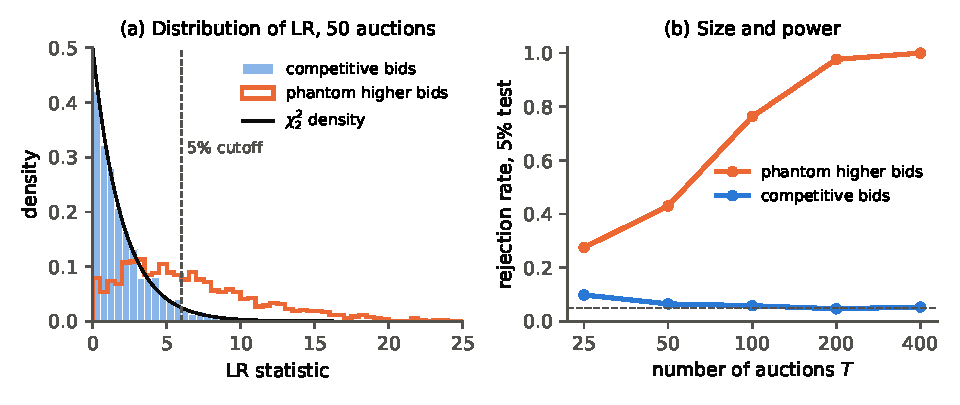
\includegraphics[width=\textwidth]{figures/ch13/pz_lr_sim.pdf}
\caption{Size and power of the rank-based test of \cref{cor:13-rank-lr} in simulated data. Panel (a) shows the
distribution of the likelihood ratio statistic over 2,000 samples of 50 auctions. The bars are for rankings that
follow the exploded logit, the line for rankings in which the nonwinning bids are in random order, and the curve is
the $\chi^2_2$ density. Panel (b) shows the rejection rates of the 5 percent test against the number of auctions,
with 600 samples per point. Our simulation, with sample sizes that mimic \citet{PorterZona1993}, Table~6.}
\label{fig:13-pz-sim}
\end{figure}

\subsection{Long Island highway paving: Porter and Zona (1993)}\label{sec:13-pz93}

\casehead{The question}
Can econometric tests detect a bid-rigging ring from public bid data when the ring includes only some of the
bidders? \citet{PorterZona1993} study contracts let by the New York State Department of Transportation (DOT) on
Long Island between April 1979 and March 1985. A group of firms bidding there was later named in bid-rigging suits.
The paper proposes test procedures and stresses their limits. In the authors' words, the tests ``will be poor
substitutes for a wiretap or a disclosure by a dissident ring member'' \citep[p.~1]{PorterZona1993}. They are,
however, better founded than the view that bid rotation or stable shares prove collusion.

\casehead{Institutional setting}
The DOT must award each highway contract to the lowest responsible bidder. It announces upcoming lettings in a
``Notice of Highway Lettings,'' and interested firms request plans and specifications. A ``Plan Buyers List'' of
the firms that bought plans for each job is distributed to subscribers, so each firm knows its potential rivals in
advance. On the day of the letting, sealed bids are opened and every bid and bidder is announced. The DOT checks
the low bid against its own cost estimate and then awards the contract. From April 1979 through March 1985 it
awarded about \$120 million of contracts in Nassau and Suffolk Counties, in 1969 dollars. There were 186 contracts,
161 of them below \$1 million. Sixty-six firms bid on at least one of the small contracts, but only 22 bid on jobs
above \$1 million. Four firms submitted 45 percent of the bids on those large jobs.

The authors list features of the market that facilitate collusion (WP pp.~8--12). The product is homogeneous,
because the contract defines the output, so a ring need only coordinate on price. Public announcement of bids and
bidders reveals any undercutting, and the plan buyers lists make the set of potential bidders common knowledge.
Demand was almost perfectly inelastic. With one exception, every contract was awarded to the low bidder whatever
the DOT's cost estimate, so any inflation of winning bids became profit. The exception is telling. In February
1983 the DOT solicited bids to resurface 0.8 miles of road, received eight bids with a low bid of about \$4 million,
and declined to award. When the job was rebid in May 1983, the low bid was 20 percent higher and came from the same
firm. A third letting in February 1984 drew three bids from firms that had bid both times before. The low bid was
about 10 percent above the second letting and 30 percent above the first, and the ranking of bidders never changed.
The contract had not been awarded by 1987.

Entry was difficult. Large jobs require batch concrete and asphalt plants, which incumbents owned, and newspaper
accounts report that union leaders discouraged outside bidders. Joint bids were allowed, which gave firms reasons to
communicate. Large jobs were let regularly, early each year, and usually one at a time. Such spacing limits what a
defector can earn before others retaliate. Firms bought inputs in the same markets, used the same technology and
employed members of the same unions, although backlogs and equipment differed.

\casehead{The candidate cartel}
In 1984 one of the five largest firms in the two counties was convicted in federal court of rigging bids on a Long
Island highway project that predates the sample. Four other firms were named as unindicted co-conspirators, and all
five were named in separate suits by New York State or Suffolk County. Each suit concerned a single job. The paper
treats these five firms, called Firms 2, 3, 4, 10 and 14, as a candidate ``cartel'' that may have operated in any
letting. The other bidders are called ``competitive.'' The cartel firms submitted 54 percent of the bids on larger
jobs and won 37 percent of all contracts. They also bid jointly at times (Table~1). Firms 4 and 2 did so in February
1980, with a winning bid of \$5.3 million. Firms 3 and 14 did so in June 1980 (\$7.3 million) and January 1982
(\$4.0 million), and Firms 3, 4 and 8 in November 1984 (\$8.0 million).

\Cref{tab:13-pz-cartel} shows that cartel firms regularly bid against each other on paving jobs. When Firm 2 bid,
another cartel firm also bid 88 percent of the time, and every bid by Firm 14 was accompanied by another cartel bid.
Insiders described the mechanism to a newspaper. Firms met around a conference table to review upcoming contracts
and decide ``who should get this one.'' Then ``the contractors who were tagged to be the low bidders would work out
their bid figures,'' and ``the rest of the contractors would then come up with higher bids'' \citep[p.~17]{PorterZona1993}.
Union representatives allegedly attended, communicated the low bids afterwards, and received a kickback of one percent of
the low bid on jobs won. This is a complementary bidding scheme, and the tests below are designed to detect it.

\begin{table}[htbp]
\centering
\caption{Bidding by the candidate cartel on Long Island paving jobs}\label{tab:13-pz-cartel}
\small
\begin{tabular}{@{}lccccc@{\hspace{2em}}cc@{}}
\toprule
 & \multicolumn{5}{c}{Bids also submitted by} & \multicolumn{2}{c}{Pr(another cartel bid), \%}\\
\cmidrule(lr){2-6}\cmidrule(l){7-8}
 & Firm 2 & Firm 3 & Firm 4 & Firm 10 & Firm 14 & Paving & Nonpaving\\
\midrule
Firm 2  & 48 & 37 & 34 & 1 & 11 & 88 & 75\\
Firm 3  & 37 & 86 & 56 & 1 & 15 & 79 & 55\\
Firm 4  & 34 & 56 & 71 & 2 & 14 & 89 & 80\\
Firm 10 & 1  & 1  & 2  & 3 & 1  & 67 & NA\\
Firm 14 & 11 & 15 & 14 & 1 & 20 & 100 & NA\\
\bottomrule
\end{tabular}

\smallskip
\begin{minipage}{0.92\textwidth}\footnotesize
Notes: Left panel, \citet{PorterZona1993}, Table~2: number of paving jobs on which the row firm and the column firm
both submitted individual bids. Diagonal entries are the row firm's total number of bids. Joint bids are excluded.
Right panel, Table~3: percentage of the row firm's bids on which at least one other cartel firm also bid. NA: not
available. NBER working-paper version.
\end{minipage}
\end{table}

\casehead{Two conventional indicators}
The first indicator is the stability of market shares. On paving jobs the cartel firms' annual shares varied
substantially, and Firm 10 stopped bidding early in the sample (it bid only three times). No pattern of rotation is
apparent. Newspaper accounts nonetheless report stable shares in state highway and sewer work for more than a
decade, on many jobs outside the sample. Shares on paving alone would thus give an unwarranted impression of
competition.

The second indicator is the dispersion of bids within a job. The 116 paving jobs received 347 competitive bids on
103 jobs and 228 cartel bids on 109 jobs. On the 76 jobs with at least two cartel bids, the second-lowest cartel bid
exceeded the lowest by 4.96 percent on average, measured as the mean difference in log bids. On the 75 jobs with at
least two competitive bids, the corresponding figure is 6.25 percent. Competitive bids are more numerous per job,
and \cref{ex:13-gap-uniform} shows that more bids shrink the expected gap. The comparison therefore understates
how much tighter the cartel bids are. The pattern resembles the clustering found by \citet{FeinsteinBlockNold1985}
in North Carolina highway contracts.

\casehead{Data}
The analysis uses contracts that involve paving, where the facilitating features are strongest. Mowing, painting
and traffic signal contracts are excluded. The 116 paving projects received 575 bids. Joint bids, under 2 percent of
paving bids, are dropped. Estimating the auction-specific variance $\sigma_t^2$ requires at least two competitive
bids, which leaves 75 projects with 319 competitive bids and 157 cartel bids.

The covariates measure cost differences across firms. $\mathit{BACKLOG}_{it}$ is the dollar value of DOT contracts
that firm $i$ has won but not completed, assuming completion at a constant pace over about three months. Capacity is
the largest backlog the firm carried in the sample, $\mathit{CAP}_i = \max_t \mathit{BACKLOG}_{it}$, and enters with
its square $\mathit{CAPSQ}$. $\mathit{NOBACK}$ marks noncartel firms that never won, for which $\mathit{CAP} = 0$.
Utilization is $\mathit{UTIL}_{it} = \frac{\mathit{BACKLOG}_{it}}{\mathit{CAP}_i}$ (zero when $\mathit{CAP}_i = 0$),
and enters with its square $\mathit{UTILSQ}$. $\mathit{ISLAND}$ marks firms headquartered on Long Island, which
includes all cartel firms. No job-specific data are available, not even the engineers' estimates. The dependent
variable is the log bid, in hundreds of thousands of 1969 dollars. The mean competitive bid was \$450,000 and the mean
cartel bid \$713,000.

\casehead{Model and estimating equations}
The competitive model is \cref{asm:13-competitive-bidding}, with cost distributions allowed to differ across firms
and jobs. Equilibrium bids satisfy \eqref{eq:13-proc-foc}, and the bid rule \eqref{eq:13-pz-bid} approximates the
equilibrium bid function. It imposes two restrictions. Firms respond in the same way to the observed covariates, and
all job-level heterogeneity is captured by the auction effect $\alpha_t$. The authors emphasize between-firm rather
than between-job variation because they have no job characteristics.

The bid levels are estimated by feasible generalized least squares in two steps. First, ordinary least squares on
the competitive bids, with a dummy for each auction, gives residuals $\hat\epsilon_{it}$. The auction variance is
estimated by the mean squared residual of the competitive bids in that auction,
\begin{equation}\label{eq:13-pz-sigma}
  \hat\sigma_t^2 = \frac{1}{n^{c}_t}\sum_{i \in \mathcal{N}^{c}_t}\hat\epsilon_{it}^{\,2},
\end{equation}
where $\mathcal{N}^c_t$ is the set of $n^c_t$ competitive bidders. Second, every observation is divided by
$\hat\sigma_t$ and the auction-dummy regression is run again. The same weights are used for three samples: all
bids, competitive bids, and cartel bids. If all bids are competitive, the three regressions estimate the same
$\beta$. If cartel bids are not competitive, only the competitive regression is consistent. A Chow test compares
the pooled regression with the two separate ones.

The rank analysis applies \cref{prop:13-exploded-logit} with $Z_{it} = -\frac{x_{it}}{\hat\sigma_t}$. It is run
separately on the ranking of competitive bids and on the ranking of cartel bids among themselves. Within each
group, the coefficients are estimated from all ranks, from the lowest rank only and from the higher ranks only,
and \cref{cor:13-rank-lr} gives the test.

\casehead{Identification}
Within an auction, bidders differ in backlog, capacity and location, and this variation identifies $\beta$. The
auction effects absorb the size, type and location of the job, which are unobserved. The rank likelihood removes
them altogether. The test for collusion rests on an asymmetry between cartel bids. A designated cartel winner must
still beat the outsiders, so it trades a higher margin against a lower probability of winning, as a competitive
bidder does. Complementary bids are designed to lose and need not respond to costs. Under phantom bidding, the
determinants of the lowest cartel bid should therefore differ from those of the higher cartel bids. The same test
applied to competitive bids is a placebo. Passing it makes it less likely that the model omits a variable that
affects high and low bids differently. The test is agnostic about how the ring chooses its winner.

\casehead{Results: bid levels}
\Cref{tab:13-pz-t4} reproduces the generalized least squares estimates. The competitive model fits well. The Wald
statistic for the six covariates is 494.7, against a $\chi^2_6$ distribution. Long Island firms bid about 3 percent
less than other firms, although the coefficient is imprecise. Bids first fall and then rise with utilization. The
effect of utilization $u$ on the log bid is $-0.0973u + 0.1720u^2$. It equals $-0.014$ at $u = 0.3$ and $0.075$ at
full capacity, and it reaches its minimum at $u = 0.28$ (our computation). These values match the paper's
statements that bids are about 1.5 percent lower at 30 percent utilization and 7.5 percent higher at full capacity. Bids also fall and then rise
with capacity, with only one firm beyond the minimum.

\begin{table}[htbp]
\centering
\caption{Generalized least squares estimates of the log bid equation, Long Island paving}\label{tab:13-pz-t4}
\small
\begin{tabular}{@{}lccc@{}}
\toprule
 & All firms & Competitive firms & Cartel firms\\
\midrule
$\mathit{UTIL}$   & $-0.0053$ & $-0.0973$ & $0.1991$\\
                  & (0.2) & (2.8) & (1.2)\\
$\mathit{UTILSQ}$ & $0.0358$ & $0.1720$ & $-0.1143$\\
                  & (1.0) & (4.0) & (0.8)\\
$\mathit{NOBACK}$ & $-0.0010$ & $-0.0178$ & \\
                  & (0.1) & (1.6) & \\
$\mathit{CAP}$    & $0.1666$ & $-1.2691$ & $1.8225$\\
                  & (1.8) & (10.4) & (4.6)\\
$\mathit{CAPSQ}$  & $-0.4430$ & $4.8519$ & $-2.9029$\\
                  & (2.1) & (13.0) & (4.4)\\
$\mathit{ISLAND}$ & $-0.0288$ & $-0.0334$ & \\
                  & (0.6) & (1.2) & \\
\midrule
Observations       & 476 & 319 & 157\\
Degrees of freedom & 395 & 238 & 81\\
Wald statistic     & 21.9 & 494.7 & 28.4\\
\bottomrule
\end{tabular}

\smallskip
\begin{minipage}{0.86\textwidth}\footnotesize
Notes: Reproduced from \citet{PorterZona1993}, Table~4 (NBER working-paper version). Absolute values of
$t$-statistics in parentheses, as in the paper. Auction-specific constants included but not reported. All
regressions use the auction variance weights estimated from competitive bids. Coefficients of $\mathit{CAP}$ and
$\mathit{CAPSQ}$ are scaled up by $10^4$ and $10^8$. $\mathit{NOBACK}$ and $\mathit{ISLAND}$ are not identified for
cartel firms. The Wald statistic tests the joint significance of the reported coefficients.
\end{minipage}
\end{table}

The cartel estimates look very different. Utilization enters with the opposite curvature, and capacity enters
with the opposite signs, significantly so. Many cartel coefficients do not have the expected sign. The Chow test
statistic is $F(76, 319) = 9.38$, with a $p$-value below $10^{-40}$ (our computation), so bids from cartel firms
differ statistically from competitive bids. The degrees of freedom reveal what the test compares. The denominator,
319, is the sum of the residual degrees of freedom of the two separate regressions, $238 + 81$. The numerator, 76,
equals the 4 cartel slopes plus 72 cartel auction constants (our reading of Table~4). The Chow test therefore
compares the levels of cartel and competitive bids within auctions as well as their slopes.

\casehead{Results: bid ranks}
\Cref{tab:13-pz-tests} reproduces the rank-based estimates. For competitive bids, the estimates are stable across
ranks. Capacity matters with similar coefficients in the lowest rank and in the higher ranks ($-1.641$ and $-2.100$
for $\mathit{CAP}$, 6.517 and 7.020 for $\mathit{CAPSQ}$). The likelihood ratio statistic is
\begin{equation*}
  LR^{\mathrm{comp}} = 2\,\bigl[-89.85 - 199.4 - (-291.4)\bigr] = 4.30 ,
\end{equation*}
against a $\chi^2_6$ distribution, with $p = 0.64$ (our computation). The paper reports that the statistic ``is
significant at about the 36 percent level,'' which is the value of the $\chi^2_6$ distribution function. Competitive
bids appear to be generated by the same process whether or not they are low.

\begin{table}[htbp]
\centering
\caption{Rank-ordered logit estimates for competitive and cartel bids, Long Island paving}\label{tab:13-pz-tests}
\small
\setlength{\tabcolsep}{5pt}
\begin{tabular}{@{}lcccccc@{}}
\toprule
 & \multicolumn{3}{c}{Competitive bids (Table~5)} & \multicolumn{3}{c}{Cartel bids (Table~6)}\\
\cmidrule(lr){2-4}\cmidrule(l){5-7}
 & All ranks & Low rank & Higher ranks & All ranks & Low rank & Higher ranks\\
\midrule
$\mathit{UTIL}$   & $-0.0070$ & $0.0161$ & $-0.0522$ & $0.0429$ & $0.2107$ & $0.2310$\\
                  & (0.1) & (0.1) & (0.3) & (0.3) & (1.0) & (0.6)\\
$\mathit{UTILSQ}$ & $0.0986$ & $0.0534$ & $0.1596$ & $-0.0112$ & $-0.1128$ & $-0.4300$\\
                  & (0.8) & (0.3) & (1.0) & (0.1) & (0.6) & (0.9)\\
$\mathit{NOBACK}$ & $-0.0283$ & $0.0089$ & $-0.0454$ & & & \\
                  & (1.0) & (0.2) & (1.3) & & & \\
$\mathit{CAP}$    & $-1.888$ & $-1.641$ & $-2.100$ & $0.4306$ & $1.101$ & $-2.537$\\
                  & (3.8) & (2.4) & (3.0) & (0.9) & (1.3) & (1.6)\\
$\mathit{CAPSQ}$  & $6.869$ & $6.517$ & $7.020$ & $-0.8473$ & $-1.904$ & $3.861$\\
                  & (3.9) & (2.6) & (2.9) & (0.9) & (1.2) & (1.4)\\
$\mathit{ISLAND}$ & $-0.0182$ & $-0.0759$ & $0.1016$ & & & \\
                  & (0.3) & (0.9) & (0.9) & & & \\
\midrule
Choice sets    & 244 & 75 & 169 & 85 & 50 & 35\\
Log likelihood & $-291.4$ & $-89.85$ & $-199.4$ & $-73.97$ & $-44.58$ & $-24.92$\\
LR test & \multicolumn{3}{c}{4.30 ($\chi^2_6$), $p = 0.64$} & \multicolumn{3}{c}{8.94 ($\chi^2_4$), $p = 0.063$}\\
\bottomrule
\end{tabular}

\smallskip
\begin{minipage}{0.95\textwidth}\footnotesize
Notes: Reproduced from \citet{PorterZona1993}, Tables~5 and~6 (NBER working-paper version). Absolute
$t$-statistics in parentheses. Coefficients of $\mathit{CAP}$ and $\mathit{CAPSQ}$ scaled up by $10^4$ and $10^8$. A
choice set is one factor of \eqref{eq:13-rank-likelihood}: an auction with $n$ ranked bids contributes one low-rank
and $n-2$ higher-rank choice sets. The $p$-values are our computation from the reported statistics.
\end{minipage}
\end{table}

For cartel bids the picture changes. The likelihood ratio statistic is
\begin{equation*}
  LR^{\mathrm{cartel}} = 2\,\bigl[-44.58 - 24.92 - (-73.97)\bigr] = 8.94 ,
\end{equation*}
against a $\chi^2_4$ distribution, because $\mathit{NOBACK}$ and $\mathit{ISLAND}$ are not identified. The $p$-value
is 0.063 (our computation), which the paper describes as significance ``at about the 94 percent level.'' The authors
reject the null hypothesis of no phantom bidding and conclude that cartel bids are generated by a different process
depending on whether they are low or not. The bookkeeping of the samples is informative. The 85 cartel choice sets
come from 50 auctions with two or more cartel bids, so these auctions contain 135 cartel bids, and only 35 choices
inform the higher-rank coefficients (our computation).

Two further features of the estimates deserve attention. The cartel rank estimates resemble the cartel bid-level
estimates of \cref{tab:13-pz-t4} and differ from all the competitive estimates. The two methods are also mutually
consistent for competitive bids. Under \eqref{eq:13-rank-index} the rank coefficients should equal
$\frac{\pi}{\sqrt6} \approx 1.28$ times the bid-equation coefficients. Scaled by this factor, the
competitive estimates of $\mathit{CAP}$ and $\mathit{CAPSQ}$ in \cref{tab:13-pz-t4} are $-1.63$ and 6.22 (our
computation). Given their standard errors, they are close to the rank estimates of $-1.89$ and 6.87. The small
utilization coefficients fail this check, but they are imprecise in the rank model.

\casehead{Robustness}
The paper reports few robustness checks beyond the competitive-rank test, which serves as a specification check.
The agreement between bid-level and rank-based results for each group of firms is a second check. The authors argue
that their classification is conservative. If some ring members were classified as competitive, the competitive
benchmark would be contaminated, which works against finding a difference.

\casehead{Interpretation}
Competitive bids are related to backlog and capacity at every rank, as cost-based bidding requires. The ranking of
the higher cartel bids does not reflect the same cost measures, and it differs from the determinants of the lowest
cartel bid. This is the footprint of complementary bids that are designed to lose. Together with the frequency of
cartel firms bidding against one another and the tight clustering of their bids, the evidence fits the scheme that
insiders described. The authors conclude that, since they have no reason to believe the difference is structural,
they ``may have found evidence of cartel activity'' \citep[p.~36]{PorterZona1993}.

\casehead{Critiques and limitations}
Several limitations follow from the design.
\begin{enumerate}[label=(\arabic*)]
\item Ring membership is not random. Cartel firms were larger, with a mean bid of \$713,000 against \$450,000, and
all were based on Long Island. Their bids could differ for structural reasons. The passing competitive-rank test
argues against general misspecification, but it cannot rule out effects specific to these firms.
\item The rank test is weak. The rejection relies on 35 higher-rank choices and has a $p$-value of 0.063. The
simulation in \cref{fig:13-pz-sim} suggests a power of about one half at this sample size even when the higher bids
ignore costs entirely.
\item The weights and standardized regressors use $\hat\sigma_t$, estimated in some auctions from just two
competitive bids. The reported standard errors do not account for this first step.
\item The covariates are crude. Backlog assumes three-month completion, there are no job characteristics, and the
model assumes independent private costs with a common response to the covariates.
\item The designated winner need not be the lowest-cost member. The cartel low-rank coefficients on capacity have
signs opposite to the competitive ones, although they are imprecise. This is consistent with a winner chosen by
turns or by equity criteria (our reading). The test remains valid in that case, because it only requires the higher
bids to be uninformative about costs.
\item A ring can adapt. If the procedure were announced, an effective cartel could scale all its bids by a common
factor, so that its ranking matches cost rankings. A noninclusive ring would then look like a group of firms with
different costs \citep[p.~36]{PorterZona1993}. \citet[pp.~246--247]{MarshallMarx2012} make the same point. They
call the rank test a plus factor that is not substantive, because a ring can alter its losing bids at no cost to
its mechanism (\cref{sec:13-market-evidence}).
\end{enumerate}

\casehead{Contribution}
The paper turned the detection of bid rigging into a problem of testing a competitive model against a specific
footprint of collusion. Its central idea is that designated and complementary bids obey different economic logic,
and that firms outside the ring provide a benchmark for the competitive model. The rank-ordered logit lets the
test ignore unobserved job characteristics. Later work, including \citet{PorterZona1999} and \citet{BajariYe2003},
follows the same logic of a competitive model, a control group and scheme-specific restrictions.
\Cref{ch:auction-empirics} returns to tests for collusion based on structural auction models.

\subsection{Ohio school milk: Porter and Zona (1999)}\label{sec:13-pz99}

\casehead{The question}
Did dairies around Cincinnati collude in school milk auctions in the 1980s, and by how much did collusion raise the
prices paid by school districts? In \emph{State of Ohio v.\ Louis Trauth Dairy, Inc., et al.}, the State charged
thirteen dairies with collusion in school milk auctions from 1980 through 1990. The case settled before trial.
\citet{PorterZona1999} adapt their reports for the plaintiff. Unlike the Long Island data, the Ohio data describe the
districts and the contract terms, so both the decision to bid and the level of the bid can be modeled.

\casehead{Setting}
Ohio has more than 600 school districts. Each district solicits bids between May and August for the supply of milk
in half pints during the next school year. A district might announce, for example, that it expects to buy 50,000 half
pints of whole white milk and 30,000 of whole chocolate milk, enough for about 450 students. Bidders submit a list of
prices, and the district may require coolers, straws or napkins, or allow escalator clauses that index prices to raw
milk. The low bidder usually wins.

Demand is insensitive to price. Using 609 districts in May 1990, the authors regress the log of half pints bought on
log enrollment and the log of the standardized price (WP p.~6, footnote 4). The estimates are
\begin{equation*}
  \ln q = 2.69 + 1.029 \ln(\text{enrollment}) + 0.21 \ln(\text{price}), \qquad R^2 = 0.84 .
\end{equation*}
The $t$-statistics on the slopes are 56.6 and 1.4, so price has no significant effect. A firm that controls supply to a
district can therefore command a much higher price there.

Costs are similar across dairies apart from distance. Raw milk prices are regulated by location and type, and the
raw milk in a half pint costs about seven cents. Packaging costs about two cents and delivery about one cent, so total
incremental cost is about ten cents per half pint (WP pp.~6--9). A cooler adds about 0.2 cents. Suppliers are
processors, which pasteurize and package milk, or distributors, which buy from processors. School milk is under 10
percent of processors' revenues, and no plant was built to serve schools alone. Transport costs and regulation make
competition local.

\casehead{Facilitating features and the testimony}
The paper lists many features that facilitate collusion (WP pp.~10--13). Firms compete only on price, bids and
bidders are announced, and districts let contracts at different times. Staggered lettings let a ring adjust its
allocation during the season and retaliate almost at once. Demand is predictable, district boundaries make
territories easy to define, and the set of potential bidders is small and stable. Dairies meet in many markets,
which by \citet{BernheimWhinston1990} relaxes the incentive constraints that limit collusion. Firms obtained rivals'
price lists through grocery customers, dairies bought from one another, and trade associations met regularly. Price
decks assigned districts to a few price levels, and one level could serve for complementary bids.

In 1993 representatives of two dairies in southwestern Ohio confessed to rigging bids during the sample period. The
paper later identifies their testimony as that of Meyer and Coors (WP p.~28). They described a scheme of respecting
incumbency. If a cartel member had served a district the previous year, the others submitted high complementary
bids that would not undercut it, or did not bid. The specific arrangements were worked out through frequent
communication during each bidding season. The witnesses also testified that the cartel broke down in two school
years, 1983--84 and 1989--90. The authors note that territorial assignment would be the more practical scheme for
firms that are far apart.

\casehead{Data}
The State of Ohio collected bid data for as many as 509 of the roughly 600 districts from 1980 through 1990, with
about 60 bidders at some point in the sample. \Cref{tab:13-pz99-t1} summarizes the data. Of 68 processing plants
with sales in Ohio during the period, 46 supplied school milk in 1987. A map of these plants (Figure~1 of the paper)
shades areas by the concentration of plant ownership within 75 miles. The northeast is least concentrated, and
Columbus and the southern tip of the state are most concentrated. The number of plants serving districts fell from
54 to 43 between 1980 and 1990, and the number of bidding dairies from 43 to 26.

\begin{table}[htbp]
\centering
\caption{The Ohio school milk data, 1980--1990}\label{tab:13-pz99-t1}
\small
\begin{tabular}{@{}lrrrrcc@{}}
\toprule
Year & Districts & Enrollment & Plants & Dairies & Average price & Raw milk price\\
\midrule
1980 & 366 & 1,257,925 & 54 & 43 & 0.12823 & 0.0718\\
1981 & 398 & 1,379,619 & 50 & 44 & 0.12950 & 0.0769\\
1982 & 415 & 1,371,164 & 46 & 40 & 0.12954 & 0.0760\\
1983 & 436 & 1,415,281 & 48 & 40 & 0.12883 & 0.0764\\
1984 & 448 & 1,430,644 & 53 & 38 & 0.13133 & 0.0741\\
1985 & 463 & 1,460,697 & 48 & 35 & 0.13215 & 0.0708\\
1986 & 481 & 1,457,437 & 47 & 36 & 0.13042 & 0.0700\\
1987 & 494 & 1,566,591 & 46 & 33 & 0.13099 & 0.0701\\
1988 & 509 & 1,520,635 & 44 & 30 & 0.13378 & 0.0666\\
1989 & 491 & 1,564,869 & 43 & 26 & 0.13886 & 0.0708\\
1990 & 412 & 1,296,587 & 43 & 26 & 0.15751 & 0.0797\\
\bottomrule
\end{tabular}

\smallskip
\begin{minipage}{0.92\textwidth}\footnotesize
Notes: Reproduced from \citet{PorterZona1999}, Table~1 (NBER working-paper version). Districts: school
districts or cooperatives in the data. Enrollment: total enrollment in those districts. Plants: plants operated by
submitting dairies. Dairies: dairies submitting bids. Prices in dollars per half pint. The raw milk price is the
July Federal Milk Order No.~33 Class~I price, converted at 186 half pints per hundredweight.
\end{minipage}
\end{table}

Distance shapes participation. A non-defendant firm bids on 19.5 percent of the districts within 10 miles of its
plant (Table~2). The probability falls to 7.6 percent at 20 to 30 miles, 2.3 percent at 40 to 50 miles and 0.5
percent at 100 to 150 miles. The probability of winning is 13.6 percent within 10 miles. These figures
come from 2,053 bids out of 73,965 bid opportunities, of which 1,260 won. About 85 percent of suppliers serve
districts from plants less than 75 miles away. Few firms bid in any auction (Table~3). Of 3,866 auctions, 45.0
percent drew one bidder, 33.6 percent two and 18.2 percent three, with a mean of 1.8. The firm with the plant
closest to the district submitted 42.8 percent of the 6,965 bids and won 48.8 percent of the 3,511 contracts
(Table~4).

\casehead{The competitive model: bid submission}
Non-defendant firms form the \emph{control group}, whose behavior defines the competitive benchmark. A competitive
dairy decides where to bid and how much to bid. Let $d$ index districts and $t$ years. The submission decision of
firm $i$ is a probit,
\begin{equation}\label{eq:13-pz99-probit}
  S^*_{idt} = w_{idt}\gamma + u_{idt}, \qquad S_{idt} = \indic\{S^*_{idt} > 0\}, \qquad u_{idt} \sim N(0,1) .
\end{equation}
The covariates $w_{idt}$ include distance from the firm's nearest plant to the district, and a processor dummy and
its interactions. They include $\mathit{Direction}$, the share of the firm's bids placed in the quadrant where the
district lies, which proxies for route structure. They also include $\mathit{Size}$, the firm's share of Ohio
students served, dummies for the closest and second-closest plants, district enrollment, contract terms and year
effects. Three
specifications are estimated: pooled, with bidder fixed effects, and with bidder and district fixed effects. The
last has over 400 coefficients and is estimated on two halves of the districts. Its distance coefficient is
identified because plant closures change distances over time.

\Cref{tab:13-pz99-control} reports selected estimates. Processors bid more often than distributors. Distance sharply
lowers the probability of bidding, more so for processors. Firms bid more often in the direction of their existing
routes, and the closest firm is more likely to bid. \Cref{fig:13-pz99-f2} plots the predicted probability of bidding
by distance for a hypothetical control-group processor. The probability starts near or above one half at zero
distance and steps down where the firm loses its locational advantage. It is close to zero beyond 75 miles.

\casehead{The competitive model: bid levels and selection}
The bid variable is a summary price per half pint for two-percent chocolate milk. Each submitted price for another
type of milk is converted with a pairwise regression, for example of chocolate on white milk prices, and the
predictions are averaged. The bid equation is
\begin{equation}\label{eq:13-pz99-bid}
  b_{idt} = x_{idt}\beta + e_{idt}, \qquad b_{idt} \text{ observed only if } S_{idt} = 1 ,
\end{equation}
with $(e_{idt}, u_{idt})$ independent of the regressors $(x_{idt}, w_{idt})$ and bivariate normal with mean zero,
$\Var(e_{idt}) = \sigma_e^2$, $\Var(u_{idt}) = 1$ and correlation $\varrho$. The conditional distribution of the
errors given the regressors is then this fixed bivariate normal. Bids are observed only for firms that chose to bid,
so ordinary least squares on submitted bids is biased if $\varrho \neq 0$.

\begin{lemma}[Selection correction]\label{lem:13-heckman}
In the model \eqref{eq:13-pz99-probit}--\eqref{eq:13-pz99-bid},
\begin{equation}\label{eq:13-heckman}
  \E\bigl[b_{idt} \mid x_{idt}, w_{idt}, S_{idt} = 1\bigr] = x_{idt}\beta + \varrho\,\sigma_e\,\lambda(w_{idt}\gamma),
  \qquad \lambda(z) = \frac{\phi(z)}{\Phi(z)} ,
\end{equation}
where $\phi$ and $\Phi$ are the standard normal density and distribution function, and $\lambda$ is the
\emph{inverse Mills ratio}.
\end{lemma}

\begin{proof}
Condition on $(x, w)$ throughout. Since the errors are independent of the regressors, the pair $(e, u)$ keeps its
bivariate normal distribution given $(x, w)$. For a bivariate normal pair with mean zero and $\Var(u) = 1$, the
regression of $e$ on $u$ is linear, $\E[e \mid u] = \varrho\sigma_e u$. Since $S = 1$ exactly when $u > -w\gamma$,
iterated expectations give
$\E[e \mid u > -w\gamma] = \varrho\sigma_e\,\E[u \mid u > -w\gamma]$. Write $a = w\gamma$. Using $\phi'(u) = -u\phi(u)$,
\begin{equation*}
  \E[u \mid u > -a] = \frac{\int_{-a}^{\infty}u\,\phi(u)\,du}{1 - \Phi(-a)}
  = \frac{\bigl[-\phi(u)\bigr]_{-a}^{\infty}}{\Phi(a)} = \frac{\phi(-a)}{\Phi(a)} = \frac{\phi(a)}{\Phi(a)} ,
\end{equation*}
where the last two steps use the symmetry of the normal distribution. Adding $x\beta$ gives \eqref{eq:13-heckman}.
\end{proof}

The two-step estimator of \citet{Heckman1979} estimates the probit, forms $\hat\lambda_{idt} = \lambda(w_{idt}\hat\gamma)$,
and regresses submitted bids on $x_{idt}$ and $\hat\lambda_{idt}$. The coefficient on $\hat\lambda$ estimates
$\varrho\sigma_e$ (\cref{app:econometrics}). Identification does not rest on the normal functional form alone,
because several probit regressors are excluded from the bid equation. Comparing Tables~6 and~7 of the paper,
$\mathit{Direction}$ and its interactions, $\mathit{Size}$ and its interactions, and the second-closest dummy shift
participation but not the bid. Route structure and scale plausibly affect the cost of adding a district to a delivery
schedule, and hence the decision to bid, more than the bid itself. This exclusion is nonetheless an assumption.

\begin{table}[htbp]
\centering
\caption{The competitive benchmark: control-group submission and bid equations}\label{tab:13-pz99-control}
\small
\begin{tabular}{@{}lcccc@{}}
\toprule
 & \multicolumn{2}{c}{Base model} & \multicolumn{2}{c}{Bidder fixed effects}\\
\cmidrule(lr){2-3}\cmidrule(l){4-5}
 & Coefficient & $t$ & Coefficient & $t$\\
\midrule
\multicolumn{5}{@{}l}{\textit{Panel A. Probit for bid submission (Table~6)}}\\
Distance                      & $-0.015453$ & $-10.1$ & $-0.022971$ & $-12.4$\\
Processor                     & 1.778220 & 18.6 & 1.689650 & 10.4\\
Processor $\times$ Distance   & $-0.035257$ & $-15.4$ & $-0.047488$ & $-13.2$\\
Direction                     & 1.146110 & 16.1 & 1.272590 & 15.5\\
Direction $\times$ Distance   & 0.005570 & 3.6 & 0.013020 & 7.0\\
Size                          & 27.876500 & 17.0 & 12.202800 & 4.6\\
Closest                       & 0.370670 & 9.9 & 0.329990 & 7.3\\
Second closest                & 0.089160 & 1.6 & 0.189010 & 3.0\\
District enrollment           & $-0.000013$ & $-4.2$ & $-0.000011$ & $-3.4$\\
Log likelihood                & \multicolumn{2}{c}{$-5964$} & \multicolumn{2}{c}{$-5052$}\\
Observations (parameters)     & \multicolumn{2}{c}{73,965 (25)} & \multicolumn{2}{c}{73,965 (89)}\\
\midrule
\multicolumn{5}{@{}l}{\textit{Panel B. Bid level with selection correction, dollars per half pint (Table~7)}}\\
Constant                      & 0.123542 & 59.5 & 0.128517 & 33.9\\
Distance                      & 0.000027 & 2.3 & 0.000004 & 0.3\\
Processor $\times$ Distance   & 0.000009 & 0.6 & 0.000065 & 2.9\\
Processor                     & $-0.002200$ & $-3.1$ & $-0.001300$ & $-0.7$\\
Closest                       & 0.003535 & 4.1 & 0.000494 & 0.6\\
Closest $\times$ Distance     & $-0.000069$ & $-2.3$ & $-0.000002$ & $-0.1$\\
Inverse Mills ratio           & 0.001713 & 2.9 & 0.001586 & 2.6\\
Fixed bid                     & 0.002334 & 3.1 & 0.001174 & 2.0\\
Escalator                     & $-0.003030$ & $-3.5$ & $-0.000890$ & $-1.3$\\
Year 1990                     & 0.031683 & 31.0 & 0.032510 & 36.1\\
$R^2$ (RMSE)                  & \multicolumn{2}{c}{0.4891 (0.009540)} & \multicolumn{2}{c}{0.7337 (0.007000)}\\
Observations                  & \multicolumn{2}{c}{2,053} & \multicolumn{2}{c}{2,053}\\
\bottomrule
\end{tabular}

\smallskip
\begin{minipage}{0.92\textwidth}\footnotesize
Notes: Selected rows of \citet{PorterZona1999}, Tables~6 and~7, columns (a)--(d) (NBER working-paper version). Signed $t$-statistics as in the paper. Both equations also include contract terms, delivery and
cooperative variables, and the bid equation includes year effects for 1981--1990. The tables also report a
specification with bidder and district fixed effects with similar coefficients of interest. The inverse Mills ratio
in each bid equation uses the corresponding probit.
\end{minipage}
\end{table}

Panel B of \cref{tab:13-pz99-control} shows the bid results. The coefficient on the inverse Mills ratio is positive.
Since $\lambda$ falls as the probability of bidding rises, firms that are likely to submit a bid tend to bid low.
Bids rise with distance. Table~8 of the paper reports the derivative of the predicted bid with respect to distance,
including the effect that runs through the selection term. For a firm that is not the closest supplier, the base
model gives 0.0096 dollars per half pint per hundred miles. The specifications with bidder effects and with bidder
and district effects give 0.0154 and 0.0194. The direct distance coefficients in column (a) imply only 0.0036 dollars per hundred miles for
a processor (our computation). Most of the base-model gradient therefore appears to work through selection (our
reading). As distance rises, the probability of bidding falls, $\lambda$ rises and the predicted bid rises with it. \Cref{fig:13-pz99-f3} plots
the predicted bid against distance. A bid 100 miles away is over a penny higher than a bid next to the plant.
Moderate increases in distance raise bids by about ten percent (WP pp.~20 and~24). With bidder effects, an escalating
bid is about 0.2 cents lower than a fixed bid ($0.001174 + 0.000890$). The 1990 year effect of about three cents
reflects the jump in the raw milk price that year (\cref{tab:13-pz99-t1}).

\begin{figure}[htbp]
\centering
\begin{subfigure}{0.78\textwidth}
\centering
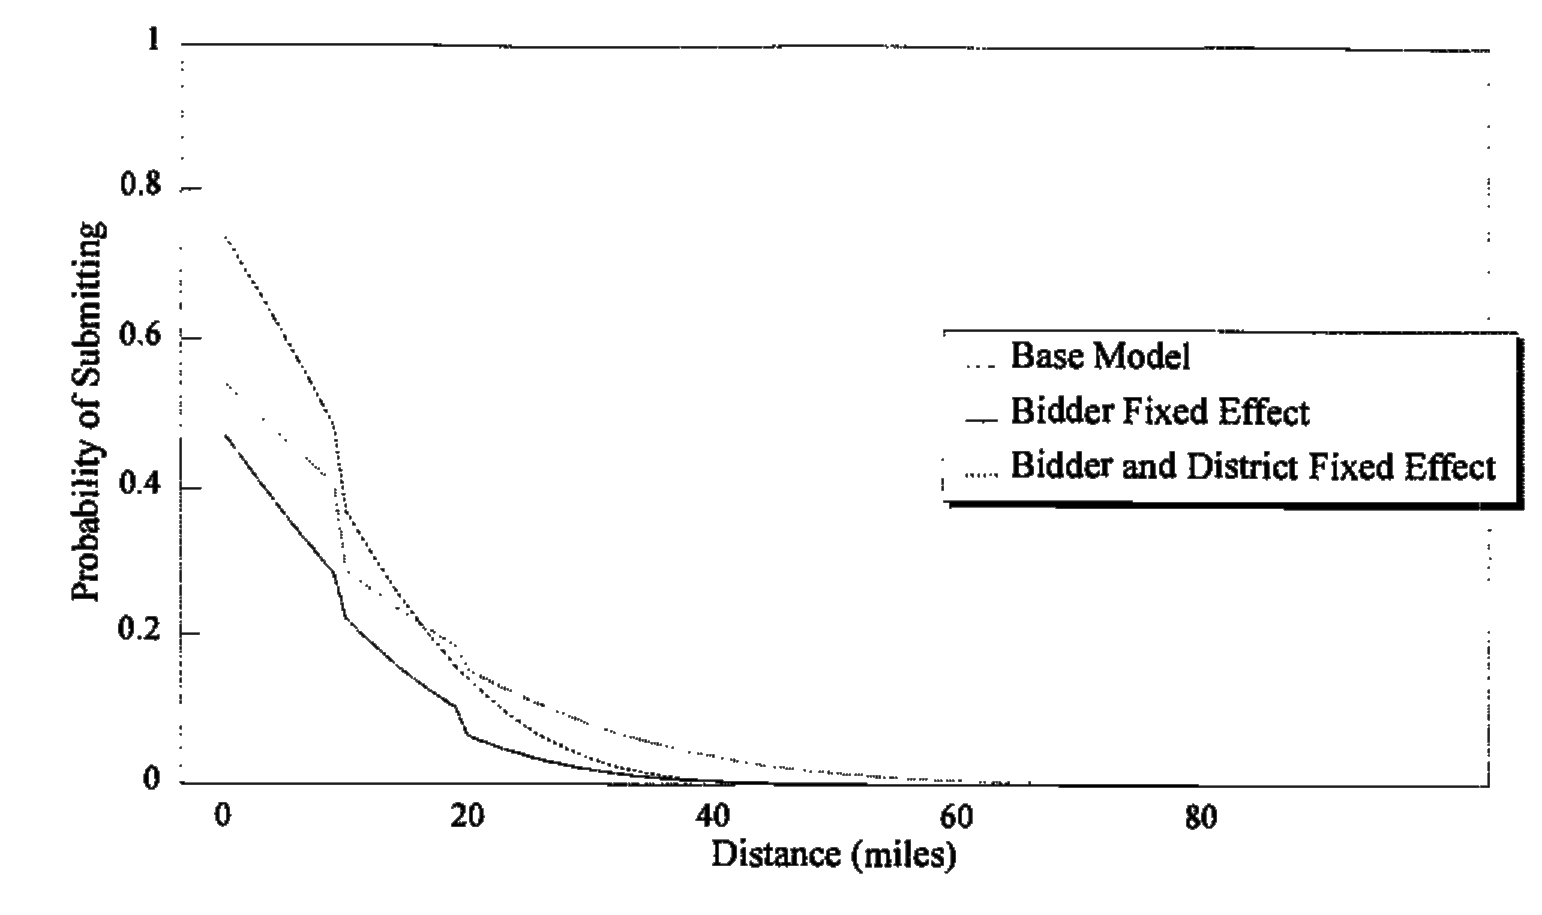
\includegraphics[width=\textwidth]{figures/ch13/pz99_fig2.png}
\caption{Predicted probability of submitting a bid}\label{fig:13-pz99-f2}
\end{subfigure}

\medskip
\begin{subfigure}{0.78\textwidth}
\centering
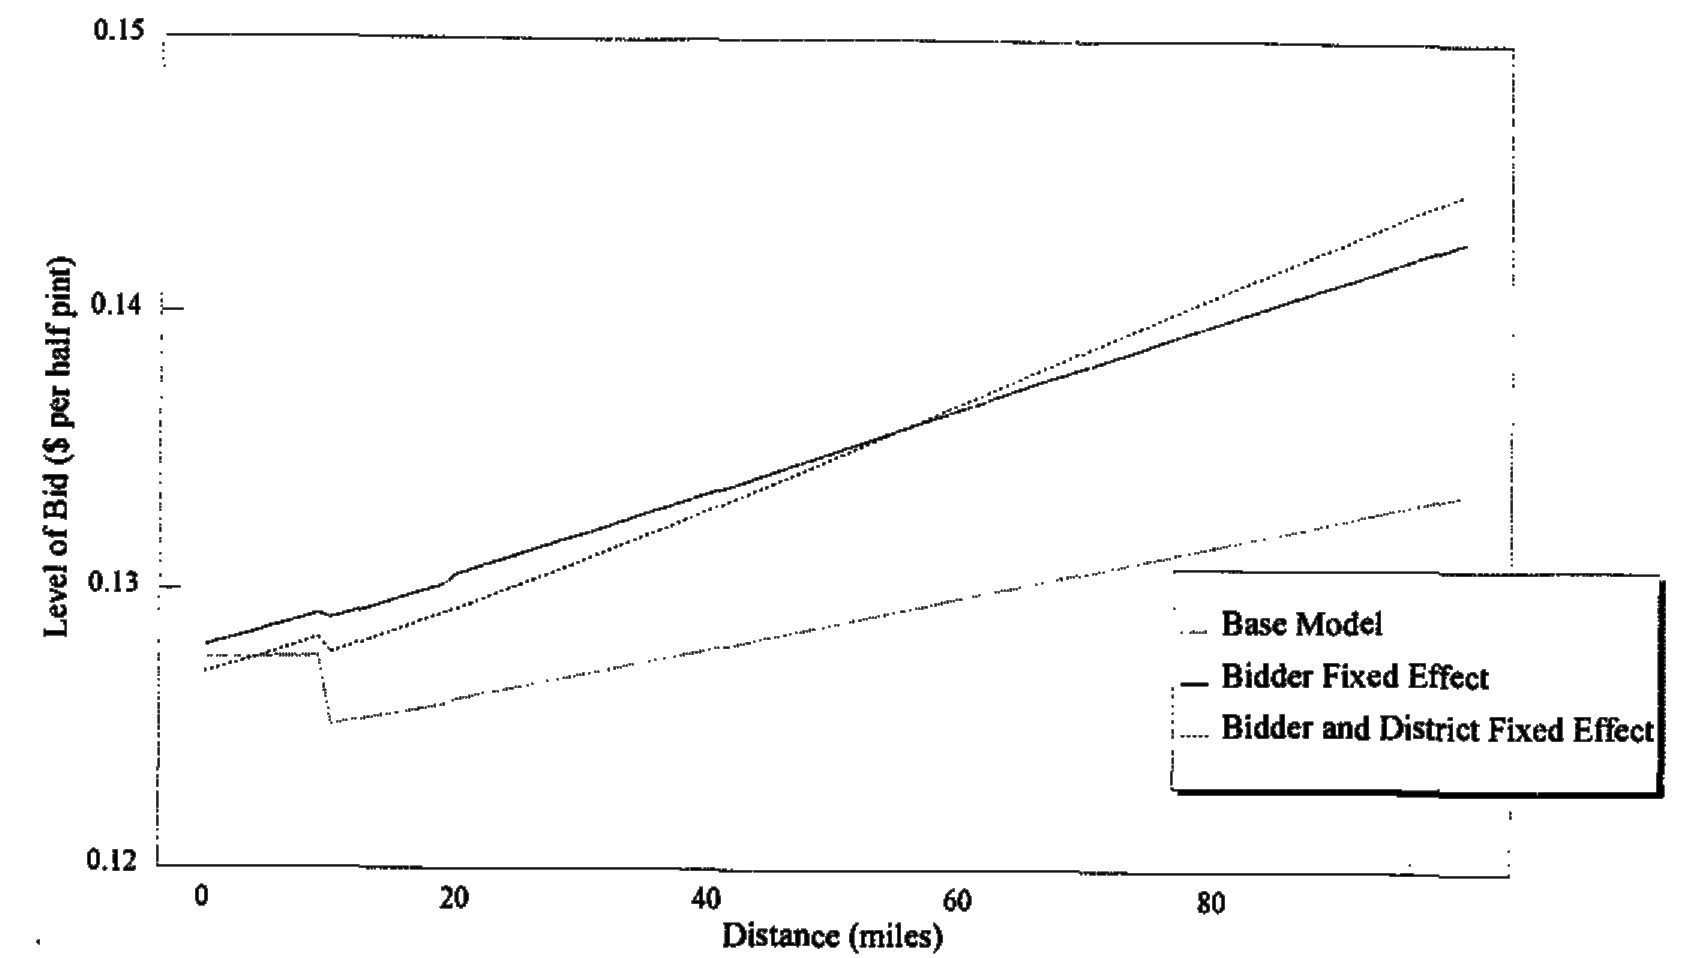
\includegraphics[width=\textwidth]{figures/ch13/pz99_fig3.png}
\caption{Predicted level of submitted bids, dollars per half pint}\label{fig:13-pz99-f3}
\end{subfigure}
\caption{The competitive benchmark in Ohio school milk: predictions for a hypothetical control-group processor by
distance from its plant, under the three specifications. Variables unrelated to distance are at their means, the
firm is the closest supplier within 10 miles and the second closest between 10 and 20 miles. The steps occur where
the firm loses these positions. The bidder fixed-effects curves are solid. In panel (a) the base model is the dotted
curve with the longest tail, and in panel (b) it is the lowest curve beyond 10 miles. The scans are darkened for
legibility. Source: \citet{PorterZona1999}, Figures~2 and~3 (NBER working-paper version).}
\label{fig:13-pz99-f23}
\end{figure}

The authors conclude that the control group bids in a way consistent with competition in a spatial market where
each firm has some local market power. Bids rise with distance, and firms rarely bid far from their plants.

\casehead{Defendants versus the control group}
The paper studies six southwestern Ohio defendants: Beatrice, Borden, Coors Brothers, H.~Meyer, Louis Trauth and
Meadow Gold. Beatrice and Meadow Gold are the same firm bidding under two names. Two tests ask whether each defendant
follows the control-group model.

The first test concerns submission. For each defendant, the authors append its submission data to the control-group
data and estimate the probit twice. Under the null hypothesis the defendant shares the control group's slopes but
has its own intercept. Under the alternative it has its own slopes. The likelihood ratio statistic is
$2(\ell^{\mathrm{alt}} - \ell^{\mathrm{null}})$. The second test concerns bid levels. For each defendant the residual
$r_{idt} = b_{idt} - x_{idt}\hat\beta^{\mathrm{control}}$ is regressed on $x_{idt}$ and a constant. Under the null
hypothesis of identical slopes, with a possibly different intercept, the slope coefficients of this regression are
zero, and an $F$ test checks this. The authors describe it as a Lagrange multiplier test chosen for convenience.

\Cref{tab:13-pz99-tests} reports both tests. Every defendant rejects the control-group submission model at the 1
percent level. For Borden, for example, the statistic is 445.9 with 20 degrees of freedom, against a 1 percent
point of 37.6 (our computation). The bid-level test rejects for every defendant except bids under the Beatrice
name. That test uses few observations, and the same firm's many bids under the Meadow Gold name reject. Results for
the fixed-effects specifications lead to the same conclusions. The authors stress that behavioral differences are
not necessarily anticompetitive. The question is how the defendants differ.

\begin{table}[htbp]
\centering
\caption{Southwestern Ohio defendants compared with the control group}\label{tab:13-pz99-tests}
\small
\begin{tabular}{@{}lccccc@{}}
\toprule
 & \multicolumn{1}{c}{Submission} & \multicolumn{2}{c}{Bid level} & \multicolumn{2}{c}{Deviation at 0--10 miles}\\
\cmidrule(lr){2-2}\cmidrule(lr){3-4}\cmidrule(l){5-6}
Defendant & LR (df) & $F$ (df) & $p$-value & Submissions & Bid\\
\midrule
Beatrice       & 157.9 (18) & 1.09 (19, 78)  & 0.3774 & $-13.7\%$ $<$ & $-4.9\%$ $<$\\
Borden         & 445.9 (20) & 10.13 (26, 386) & 0.0000 & $-0.2\%$ & $1.9\%$ $>$\\
Coors Brothers & 187.8 (19) & 5.02 (25, 102) & 0.0000 & $24.2\%$ $>$ & $9.3\%$ $>$\\
H.~Meyer       & 477.5 (20) & 11.53 (26, 384) & 0.0000 & $5.6\%$ $>$ & $2.7\%$ $>$\\
Louis Trauth   & 319.2 (20) & 9.66 (25, 345) & 0.0000 & $7.0\%$ $>$ & $5.5\%$ $>$\\
Meadow Gold    & 503.8 (20) & 7.09 (25, 771) & 0.0000 & $0.0\%$ & $0.1\%$\\
\bottomrule
\end{tabular}

\smallskip
\begin{minipage}{0.92\textwidth}\footnotesize
Notes: From \citet{PorterZona1999}, Tables~9--12 (NBER working-paper version), base models. LR: test
of equal probit slopes, all significant at 1 percent. $F$: test that the slopes of the regression of bid residuals
on the control-group regressors are zero. Submissions: actual minus predicted bids as a percentage of district-years
within 10 miles of the firm's plant, a difference in percentage points (Table~11). Bid: average deviation of actual from predicted bids, in percent of
the predicted bid (Table~12). $>$ ($<$): actual significantly above (below) predicted at 95 percent confidence.
\end{minipage}
\end{table}

\casehead{Where the defendants differ}
Since distance dominates the control-group model, the authors examine deviations by distance. Table~11 of the paper
tabulates actual minus predicted submissions in bands of ten miles, as a percentage of the district-years in each
band. These are differences in participation rates, so they are measured in percentage points. Coors Brothers'
actual submission rate exceeded its predicted rate by 24.2 percentage points within 10 miles of its plant and by
42.9 percentage points at 10 to 20 miles. Coors, Meyer and Trauth bid more often than predicted at distances up to about 30 miles,
and Meyer and Trauth also at some greater distances. Beatrice, Meadow Gold and Borden bid less often than predicted
within about 40 miles, where they would have a cost advantage. Borden and Meadow Gold bid more often than predicted
at 70 to 100 miles.

Table~12 tabulates bid residuals, as a percentage of the predicted bid, by regressing each firm's residuals on
distance-band indicators. Its first row is the deviation within 10 miles, and later rows are increments relative to
that row. Coors bid 9.3 percent above the prediction within 10 miles, and about 10.0 percent above it at 10 to 20
miles. For Borden, Meyer, Trauth and Meadow Gold, the deviation falls significantly with distance. Borden's bids at 70
to 80 miles, for example, are 5.1 percent lower relative to its local deviation. Under competition, local bids
should be lower than distant bids, because shipping costs are lower and the Cincinnati area has many potential
suppliers. Bids that fall with distance relative to the control group are hard to explain without collusion
\citep[p.~28]{PorterZona1999}. They fit territorial allocation near the plants and more competitive bidding farther
away.

\casehead{Correlation tests}
Under the null hypothesis of independent action based on public information, \cref{prop:13-competitive-restrictions}(ii)
implies that the unexplained parts of two firms' decisions are uncorrelated. Under complementary bidding, when one
ring member bids the others also bid, so submission residuals are positively correlated. Under territorial
allocation, when one member bids the others stay out, so the correlation is negative. For bid levels, a complementary
scheme implies that when one member bids high, the cover bids are high too.

The authors test independence of submission decisions with the Lagrange multiplier (LM) statistic of \citet{Kiefer1982}.
Its logic is easy to derive. Consider two firms facing the same district-year, with probits $S_k = \indic\{a_k +
u_k > 0\}$, $a_k = w_k\gamma_k$, $k = 1, 2$, and let $(u_1, u_2)$, independent of $(w_1, w_2)$, be standard bivariate normal with correlation
$\rho_{12}$ (a local symbol). With $q_k = 2S_k - 1$, the probability of the observed pair is
$\Phi_2(q_1a_1, q_2a_2; q_1q_2\rho_{12})$, where $\Phi_2$ is the bivariate normal distribution function. The
derivative of $\Phi_2$ with respect to its correlation argument is the bivariate normal density $\phi_2$, which at
zero correlation equals $\phi(q_1a_1)\phi(q_2a_2)$. By the chain rule and the symmetry of $\phi$, the score at
$\rho_{12} = 0$ is
\begin{equation}\label{eq:13-kiefer-score}
  \frac{\partial\ln\Pr(S_1, S_2)}{\partial\rho_{12}}\bigg|_{\rho_{12} = 0}
  = \frac{q_1q_2\,\phi(a_1)\phi(a_2)}{\Phi(q_1a_1)\,\Phi(q_2a_2)} = g_1 g_2,
  \qquad g_k = \frac{\phi(a_k)\bigl[S_k - \Phi(a_k)\bigr]}{\Phi(a_k)\bigl[1 - \Phi(a_k)\bigr]} .
\end{equation}
Here $g_k$ is the generalized residual of probit $k$. It equals $\frac{\phi(a_k)}{\Phi(a_k)}$ when $S_k = 1$ and
$-\frac{\phi(a_k)}{1-\Phi(a_k)}$ when $S_k = 0$. The test asks whether the products $g_{1m}g_{2m}$ average to zero
over district-years $m$, with the statistic
\begin{equation}\label{eq:13-kiefer-lm}
  LM = \frac{\bigl(\sum_m g_{1m}g_{2m}\bigr)^2}{\sum_m g_{1m}^2 g_{2m}^2} \xrightarrow{d} \chi^2_1 .
\end{equation}
Because $\E[g_2] = 0$, the score for $\rho_{12}$ is uncorrelated with the probit scores at $\rho_{12} = 0$, so
estimated probit coefficients can be plugged in. \Cref{tab:13-pz99-corr} reports the Spearman rank correlations of
standardized residuals $\frac{S - \hat\Phi}{\sqrt{\hat\Phi(1 - \hat\Phi)}}$ above the diagonal, with significance
from the LM test. Below the diagonal it reports Spearman correlations of bid-level residuals for district-years in
which both firms bid.

\begin{table}[htbp]
\centering
\caption{Correlations of residuals across pairs of defendants}\label{tab:13-pz99-corr}
\small
\setlength{\tabcolsep}{4.5pt}
\begin{tabular}{@{}lcccccc@{}}
\toprule
 & Beatrice & Borden & Coors & H.~Meyer & L.~Trauth & Meadow Gold\\
\midrule
Beatrice       &  & 0.0967 & 0.0491 & 0.0522$^{**}$ & 0.0627 & $-0.0343^{**}$\\
               &  & [1609] & [761] & [896] & [791] & [1609]\\
Borden         & $-0.3571$ &  & 0.1952 & 0.2129$^{**}$ & 0.2020$^{**}$ & 0.0947$^{*}$\\
               & [8] &  & [1379] & [1522] & [1410] & [2158]\\
Coors Brothers & $-1.0000$ & $-0.2571$ &  & 0.5813$^{**}$ & 0.4344$^{**}$ & 0.2059\\
               & [3] & [6] &  & [1432] & [1320] & [1193]\\
H.~Meyer       & 0.0091 & 0.2743$^{*}$ & 0.6598$^{**}$ &  & 0.5389$^{**}$ & 0.1188$^{**}$\\
               & [11] & [73] & [126] &  & [1463] & [1328]\\
Louis Trauth   & 0.9182$^{**}$ & 0.3724$^{**}$ & 0.5366$^{**}$ & 0.6674$^{**}$ &  & 0.1124$^{*}$\\
               & [11] & [51] & [114] & [267] &  & [1223]\\
Meadow Gold    & NA & 0.1634 & $-1.0000$ & 0.3539$^{**}$ & 0.6317$^{**}$ & \\
               & [0] & [59] & [2] & [69] & [58] & \\
\bottomrule
\end{tabular}

\smallskip
\begin{minipage}{0.95\textwidth}\footnotesize
Notes: Above the diagonal, \citet{PorterZona1999}, Table~13: Spearman correlations of standardized submission
residuals from the base probit, with significance from the LM test of \citet{Kiefer1982}. Below the diagonal,
Table~14: Spearman correlations of bid-level residuals from the base model. Numbers of observations in brackets.
$^{**}$ significant at 1 percent, $^{*}$ at 10 percent. NBER working-paper version.
\end{minipage}
\end{table}

The correlations are large and positive for the pairs among Coors, Meyer and Trauth. Submission residuals correlate
at 0.58 (Coors and Meyer), 0.54 (Meyer and Trauth) and 0.43 (Coors and Trauth). Their bid residuals correlate at
0.66, 0.67 and 0.54, on 126, 267 and 114 common district-years. When one of these firms bids, the others tend to bid
too, and their bids move together, beyond what proximity, size and contract terms predict. Borden is positively
correlated with Meyer and Trauth in both submissions and bids, and Meadow Gold's bids correlate with Trauth's (0.63).
Some pairs involving Beatrice rest on as few as three to eleven observations and carry little information. The bid
correlation test has little power against a pure territorial scheme, because ring members would then rarely bid in
the same district in the same year (WP p.~27, footnote 30).

\casehead{Interpretation}
The pieces fit together. Coors, Meyer and Trauth submit more bids than predicted within about 30 miles of their
plants, these bids are high, their submissions are positively correlated, and their bids move together. This is the
footprint of complementary bidding near their plants. The authors conclude that the collective behavior of these
three firms ``is best characterized as collusive'' \citep[p.~28]{PorterZona1999}, which supports the testimony of
Meyer and Coors. Beatrice, Meadow Gold and Borden refrain from bidding in their local areas, where they would have a
comparative advantage, and their bidding is correlated with Trauth's. This pattern is consistent with a
complementary bidding scheme that involves them as well.

\casehead{Damages: a collusion index}
To measure the overcharge, the authors regress the price of the winning bid on market structure and on an index of
exposure to the alleged conspiracy. Market structure is measured by the number of \emph{equivalent firms}, the
inverse of a Herfindahl index. For district $d$, let $s_{fd}$ be the fraction of school milk processing plants within
75 miles of the district that firm $f$ owns, and define
\begin{equation}\label{eq:13-pz99-equiv}
  \HHI_d = \sum_f s_{fd}^2, \qquad N^e_d = \frac{1}{\HHI_d} .
\end{equation}
With ten owners of one plant each, $N^e_d = 10$. Under collusion, the conspirators $\mathcal{C}$ with plants within
75 miles act as one owner with share $s_{\mathcal{C}d} = \sum_{f\in\mathcal{C}}s_{fd}$. The Herfindahl index becomes
\begin{equation*}
  \HHI^{\mathrm{col}}_d = \HHI_d - \sum_{f\in\mathcal{C}}s_{fd}^2 + \Bigl(\sum_{f\in\mathcal{C}}s_{fd}\Bigr)^2
  = \HHI_d + 2\sum_{\substack{f, g\in\mathcal{C}\\ f < g}}s_{fd}\,s_{gd} .
\end{equation*}
The \emph{collusion index} (the paper's ``Delta'') is the resulting loss of equivalent firms,
\begin{equation}\label{eq:13-pz99-delta}
  \Delta^{\mathrm{col}}_d = \frac{1}{\HHI_d} - \frac{1}{\HHI^{\mathrm{col}}_d} \geq 0 .
\end{equation}

\begin{example}[Computing the collusion index]\label{ex:13-pz99-delta}
Suppose six plants lie within 75 miles of a district, each with a different owner, and three owners are
conspirators. Competition gives $\HHI_d = 6 \times \frac{1}{36} = \frac{1}{6}$ and $N^e_d = 6$. Under collusion the
shares are $\frac{3}{6}$ for the conspirators and $\frac{1}{6}$ for each of the three others, so
$\HHI^{\mathrm{col}}_d = \frac{1}{4} + \frac{3}{36} = \frac{1}{3}$ and the number of equivalent firms is 3. The
collusion index is $\Delta^{\mathrm{col}}_d = 6 - 3 = 3$ (our computation).
\end{example}

The price equation, estimated by ordinary least squares on about 400 districts including districts outside
southwestern Ohio, is
\begin{equation}\label{eq:13-pz99-damages}
  \ln p_{dt} = \mu_t + z_{dt}\eta + \omega_1 N^e_{dt} + \omega_2 (N^e_{dt})^2
  + \sum_{\tau}\indic\{t = \tau\}\Bigl[a_{1\tau}\Delta^{\mathrm{col}}_{dt} + a_{2\tau}(\Delta^{\mathrm{col}}_{dt})^2
  + a_{3\tau}\Delta^{\mathrm{col}}_{dt}N^e_{dt}\Bigr] + e_{dt} .
\end{equation}
Here $p_{dt}$ is the standardized price of the winning bid, and $\mu_t$ are year effects that absorb raw milk and
packaging costs. The vector $z_{dt}$ contains the distances to the closest and second-closest plants, log
enrollment, the number of deliveries and the contract terms. The quadratic terms allow diminishing effects of competition, and the
interaction lets the effect of collusion depend on the initial level of competition. The year interactions let the
effectiveness of the conspiracy vary over time. The predicted effect of collusion is the prediction with the
collusion terms minus the prediction with all of them set to zero:
\begin{equation}\label{eq:13-pz99-effect}
  \hat m_{dt} = \hat a_{1t}\Delta^{\mathrm{col}}_{dt} + \hat a_{2t}(\Delta^{\mathrm{col}}_{dt})^2
  + \hat a_{3t}\Delta^{\mathrm{col}}_{dt}N^e_{dt} .
\end{equation}
The paper evaluates this log difference at the mean values of the variables.

The competitive part of the price equation behaves as expected (Table~16, with 3,431 observations and $R^2 = 0.6239$). One
more equivalent firm lowers the price by about 1.5 percent (coefficient $-0.0150$, $t = -5.7$). The distance to the
second-closest plant raises the price (0.0003, $t = 3.1$), as the closest firm's advantage grows. Larger districts
pay less (log enrollment $-0.0134$, $t = -11.9$), and escalator clauses lower prices ($-0.0096$, $t = -4.2$). The
distance to the closest plant has a small negative coefficient ($-0.0004$, $t = -3.6$), which the theory does not
predict.

\begin{table}[htbp]
\centering
\caption{Estimated effect of collusion on prices paid by southwestern Ohio school districts}\label{tab:13-pz99-t17}
\small
\begin{tabular}{@{}lccccc@{}}
\toprule
School year & $\hat a_{1t}$ (Delta) & $\hat a_{2t}$ (Delta$^2$) & $\hat a_{3t}$ (interaction) & Average effect & Effect given incumbency\\
 & (a) & (b) & (c) & (d) & (e)\\
\midrule
1980--81 & $-0.0014$ & $-0.0015$ & 0.00163 & 3.0\% & 3.2\%\\
1981--82 & 0.01304 & 0.01167 & 0.00103 & 11.3\% & 40.2\%\\
1982--83 & 0.02731 & 0.00225 & 0.00098 & 8.6\% & 23.2\%\\
1983--84 & 0.02995 & $-0.0097$ & 0.00156 & 4.5\% & 1.1\%\\
1984--85 & 0.02147 & 0.00106 & 0.00199 & 6.7\% & 19.7\%\\
1985--86 & 0.02684 & $-0.0023$ & 0.00122 & 5.4\% & 11.5\%\\
1986--87 & 0.02425 & 0.00173 & 0.0013 & 6.5\% & 20.5\%\\
1987--88 & 0.00368 & 0.02901 & 0.0006 & 3.3\% & 49.0\%\\
1988--89 & $-0.0227$ & 0.03636 & 0.00229 & 2.9\% & 29.4\%\\
1989--90 & $-0.0494$ & 0.0134 & 0.0041 & $-1.6\%$ & 3.4\%\\
1990--91 & $-0.0201$ & $-0.0126$ & 0.00634 & $-0.3\%$ & $-8.3\%$\\
\bottomrule
\end{tabular}

\smallskip
\begin{minipage}{0.92\textwidth}\footnotesize
Notes: Reproduced from \citet{PorterZona1999}, Table~17 (NBER working-paper version). Columns (a)--(c)
are the year-specific coefficients of \eqref{eq:13-pz99-damages}. Column (d) is the expected markup over
competitive prices for the average district in southwestern Ohio, computed at mean values as a difference in
predicted log prices. Column (e) conditions on
a defendant being the incumbent. School years as labeled in the paper.
\end{minipage}
\end{table}

\Cref{tab:13-pz99-t17} and \cref{fig:13-pz99-effects} show the estimated effects by year. The paper notes that the
effect is small in 1983--84 and after 1989 in both columns (WP p.~31). These are the two breakdowns described in the
testimony. The incumbency measure, column (e), shows them most clearly. It falls to 1.1 percent in 1983--84 and 3.4
percent in 1989--90, and it is negative in 1990--91. In the years between the breakdowns it ranges from 11.5 to 49.0
percent, and it reaches 40.2 percent in 1981--82. The average effect, column (d), shows the first breakdown less
clearly. It is 4.5 percent in 1983--84, above its values in 1980--81, 1987--88 and 1988--89. It is negative in
1989--90 and 1990--91. The authors summarize the average effect of collusion as an
increase of ``about six and one half percent,'' roughly the cost of shipping school milk about 50 miles.
The paper does not state how this average weights the years. \citet[p.~235]{ErutkuHildebrand2010} describe it as
the average ``when excluding 3 years in which the cartel was said to have broken down.'' The simple mean of
column (d) is 4.6 percent over all eleven years and 5.8 percent over 1980--81 to 1988--89. Excluding 1983--84,
1989--90 and 1990--91 gives $\frac{47.7}{8} = 6.0$ percent (our computation), so the weighting remains unstated.
Erutku and Hildebrand also report the authors' suggestion that the 6.5 percent price effect amounts to a rise of
roughly 30 percent in the markup.

\begin{figure}[htbp]
\centering
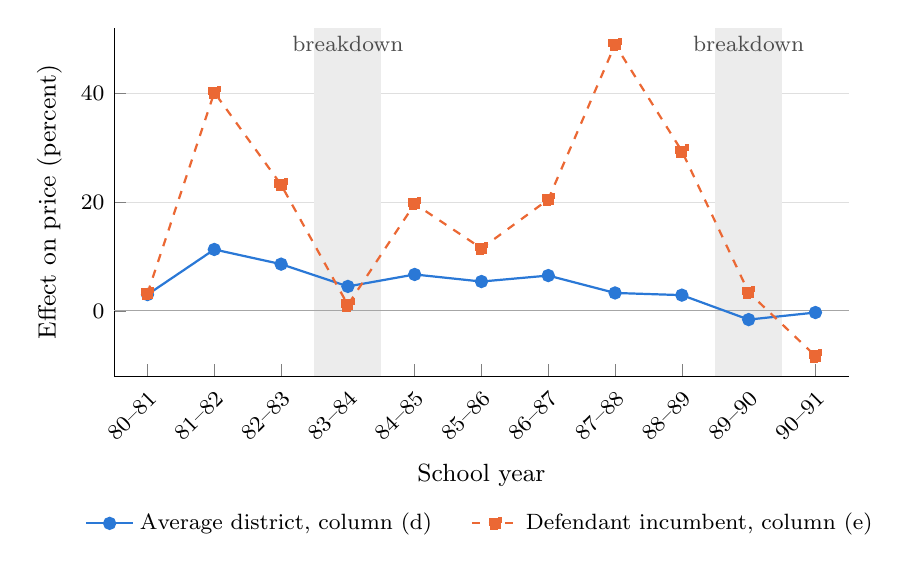
\begin{tikzpicture}
\begin{axis}[
  width=0.9\textwidth, height=6cm,
  xmin=0.5, xmax=11.5, ymin=-12, ymax=52,
  xtick={1,2,3,4,5,6,7,8,9,10,11},
  xticklabels={80--81,81--82,82--83,83--84,84--85,85--86,86--87,87--88,88--89,89--90,90--91},
  x tick label style={font=\footnotesize, rotate=45, anchor=north east},
  y tick label style={font=\footnotesize},
  xlabel={School year}, ylabel={Effect on price (percent)},
  label style={font=\small},
  legend style={font=\footnotesize, draw=none, fill=none, at={(0.5,-0.36)}, anchor=north, legend columns=2,
    /tikz/every even column/.append style={column sep=1.2em}}, legend cell align=left,
  axis lines*=left, ymajorgrids, grid style={gray!25}]
\fill[gray!15] (axis cs:3.5,-12) rectangle (axis cs:4.5,52);
\fill[gray!15] (axis cs:9.5,-12) rectangle (axis cs:10.5,52);
\draw[gray!70] (axis cs:0.5,0) -- (axis cs:11.5,0);
\addplot[thick, color={rgb,255:red,42;green,120;blue,214}, mark=*, mark size=2pt]
  coordinates {(1,3.0) (2,11.3) (3,8.6) (4,4.5) (5,6.7) (6,5.4) (7,6.5) (8,3.3) (9,2.9) (10,-1.6) (11,-0.3)};
\addlegendentry{Average district, column (d)}
\addplot[thick, dashed, color={rgb,255:red,235;green,104;blue,52}, mark=square*, mark size=2pt]
  coordinates {(1,3.2) (2,40.2) (3,23.2) (4,1.1) (5,19.7) (6,11.5) (7,20.5) (8,49.0) (9,29.4) (10,3.4) (11,-8.3)};
\addlegendentry{Defendant incumbent, column (e)}
\node[font=\footnotesize, gray!60!black, anchor=south] at (axis cs:4,46) {breakdown};
\node[font=\footnotesize, gray!60!black, anchor=south] at (axis cs:10,46) {breakdown};
\end{axis}
\end{tikzpicture}
\caption{Estimated effect of collusion on the price of school milk in southwestern Ohio, by school year. Shaded
years are the cartel breakdowns described in the testimony (1983--84 and 1989--90). Redrawn from
\citet{PorterZona1999}, Table~17, columns (d) and (e).}
\label{fig:13-pz99-effects}
\end{figure}

\begin{example}[From a log markup to damages]\label{ex:13-pz99-damages}
The dependent variable of \eqref{eq:13-pz99-damages} is the log price, so column (d) of \cref{tab:13-pz99-t17} is a
log difference, $\hat m = \ln p - \ln p^{\mathrm{bf}}$. The paper reports it as a percentage change (WP p.~31). As in
\eqref{eq:13-damages-log}, the overcharge as a share of spending is
\begin{equation*}
  \frac{p - p^{\mathrm{bf}}}{p} = 1 - e^{-\hat m} .
\end{equation*}
With $\hat m = 0.065$, the overcharge is $1 - e^{-0.065} = 6.3$ percent of spending. Reading 6.5 percent instead as a
ratio markup $\frac{p}{p^{\mathrm{bf}}} - 1$ would give $\frac{0.065}{1.065} = 6.1$ percent. A district that spent
\$100,000 on milk would have overpaid about \$6,300 (a hypothetical district, our computation). Because school milk demand is
nearly perfectly inelastic, this transfer is the whole of the district's loss.
\end{example}

The comparison with distance in the abstract can be checked against \cref{tab:13-pz99-control}. Fifty miles at the
base-model gradient of 0.0096 dollars per hundred miles adds 0.48 cents, or 3.6 percent of the mean price of 13.4
cents in \cref{tab:13-pz99-t1}. With bidder effects it adds 0.77 cents, or 5.7 percent (our computation). The authors'
own illustration is a district next to the plants of two conspirators whose nearest competitors are at least 50
miles away. Prices there could be about half a penny, or five percent, above the competitive level (WP p.~31).

\casehead{Critiques and limitations}
The evidence is a set of imperfect tests, none decisive alone. The likelihood ratio tests of equal slopes reject for
every defendant, and the authors note in footnote 15 that no single intercept represents all bidders. Such tests
would probably reject for many individual non-defendants too, so the rejections carry little weight by themselves.
The informative evidence is the pattern of deviations. Distance gradients are reversed and residuals are
correlated, and both match the testimony. Positive correlations could also arise from an omitted factor that affects
these firms alike (WP p.~27, footnote 28). The control group is assumed competitive. Collusion among non-defendants
would bias the benchmark toward the defendants' behavior and work against the tests.

The damage regression is a reduced form. Its identifying variation is the cross-sectional exposure of districts to
conspirators' plants, which is credible only if plant locations are unrelated to unobserved local cost and demand
conditions. The 75-mile radius, the plant-count shares and the quadratic forms are approximations, and the
competitive price for southwestern Ohio is predicted partly from districts elsewhere in the state. The year
pattern, which matches the breakdowns in the testimony, is the strongest validation of the index.

\casehead{Contribution}
The paper extends the Long Island design to markets in which collusion takes the form of incumbency rights and
territorial allocation. It models both the decision to bid and the level of the bid, with a selection correction. It
then matches several scheme-specific tests to the alleged scheme and builds a reduced-form damages estimate whose
time pattern can be compared with testimony. The combination of a competitive model estimated on a control group,
tests of independence across suspected firms, and damages from exposure to the ring remains a template for
procurement cases.

\casehead{Later screens}
Porter and Zona warn that a single test procedure able to detect all bid rigging is an impossible goal. Later work
has therefore developed tests aimed at particular schemes and data \citep[p.~210]{AskerNocke2021}.
\citet{BajariYe2003} test conditional independence and exchangeability (\cref{sec:13-detection-theory}).
\citet{AtheyLevinSeira2011} compare open and sealed timber auctions, as \cref{ch:auction-empirics} explains.
\citet{KawaiNakabayashi2020} exploit the rounds of Japanese national procurement auctions, as reported by
\citet[pp.~184--185]{AskerNocke2021}. When no first-round bid meets the secret reserve price, the lowest
first-round bid is announced and a second round follows. In the second round, the gap between the bids of the
first-round runner-up and the first-round winner is almost never negative. The gap between the bids of the
first-round third and second bidders often is. The first-round winner thus almost always wins again, while lower
ranks switch freely, which suggests that the winner was chosen before the auction. Applied across 2003--2006, the
test flags about 970 firms as collusive. \citet{ConleyDecarolis2016} detect groups of coordinating bidders in Italian
procurement, and \citet{OrtnerEtAl2020} develop screens that remain informative when cartels adapt to them.
\Cref{sec:12-eu-facts} uses the first two of these studies as evidence on the prevalence of collusion, and the book
does not develop the three tests further.

\section{Enforcement, Damages and What the Evidence Shows}\label{sec:13-enforcement}

The cartels of this chapter came to light in different ways, and the route matters for what they can teach. This
section describes the enforcement institutions and the selection of cartels they induce
(\cref{sec:13-institutions}). It then develops the methods used to measure the effects of collusion
(\cref{sec:13-damages}) and closes with what the evidence of the chapter shows (\cref{sec:13-synthesis}).

\subsection{Enforcement institutions and the selection of observed cartels}\label{sec:13-institutions}

\casehead{Law and penalties}
In the United States, Section~1 of the Sherman Act (1890) prohibits agreements in restraint of trade. Price fixing
is illegal per se \citep[p.~570]{Miller2010}. Section~1 is a criminal as well as a civil statute, so price fixing
and bid rigging can be prosecuted as crimes \citep[ch.~4, p.~74, footnote~13]{Kaplow2013}. Injured parties can sue for treble damages
\citep[p.~759]{Asker2010}.
In the European Union, Article~101 of the Treaty on the Functioning of the European Union prohibits cartels. The
European Commission imposes administrative fines, capped at 10 percent of a firm's turnover
\citep[p.~6]{ChenRey2013}. Page and footnote references to \citet{ChenRey2013} are to its working-paper version.
\Cref{tab:12-eu-fines} lists the largest fines the Commission has imposed. On the conventional view, liability for
price fixing requires proof of an agreement, usually through evidence of communication, and plus factors serve as
circumstantial support \citep[pp.~4, 21 and 109--110]{Kaplow2013}. \Cref{sec:12-kaplow} discusses Kaplow's critique of
this requirement, and \cref{sec:13-market-evidence} the market-based evidence itself.

\casehead{Leniency}
Proving an agreement is the hard part of enforcement, and leniency programs address it. The United States adopted a
corporate leniency program in 1978. Under the Antitrust Division's 1993 Corporate Leniency Policy, a firm that
reports before an investigation has begun receives leniency automatically if it meets six conditions. The Division
must have no information about the conduct from any other source. The firm must end its participation promptly,
cooperate fully and make restitution where possible, and its confession must be a corporate act rather than that of
individual executives. It must not have coerced others or led or originated the cartel. A firm
that misses these conditions, including one that comes forward after an investigation has begun, can still qualify
under seven alternative conditions. Four of them repeat the conditions on termination, cooperation, the corporate
confession and restitution. In addition, the firm must be the first to come forward and qualify. The Division must not yet
have evidence likely to yield a sustainable conviction, and it must judge that leniency would not be unfair to
others. \citet[p.~1]{ChenRey2013} summarize the revision as a first-informant rule and a post-investigation amnesty
rule. Eligibility after an investigation has begun thus depends on the alternative conditions.

The European Commission adopted its program in the 1996 Notice on the Non-Imposition or Reduction of Fines in
Cartel Cases. That notice reduced fines by 75 to 100 percent for a firm that reported before the Commission had
ordered an investigation. A firm that reported after such an investigation had failed to establish sufficient
grounds for proceedings could receive 50 to 75 percent. Both tiers also required the firm to be the first to adduce
decisive evidence, to end its involvement, to cooperate fully and not to have coerced others or instigated the
cartel. Other cooperation earned 10 to 50 percent. The first two
tiers are those that \citet[footnote~6]{ChenRey2013} describe. The Commission revised the program in 2002
\citep[footnote~1]{ChenRey2013} and again in its 2006 Notice on Immunity from Fines and Reduction of Fines in Cartel
Cases, which remains its framework. Under the 2006 notice, the first firm whose evidence enables an inspection or
a finding of infringement can obtain full immunity if it meets the notice's conditions. Later firms whose evidence
adds significant value receive reductions of 30 to 50 percent for the first, 20 to 30 percent for the second and up
to 20 percent for the others. Many recent prosecutions involve a whistleblower.

In the repeated-game language of \cref{ch:collusion-theory}, leniency changes both sides of a member's incentive
constraint. \citet[pp.~209--210]{AskerNocke2021} summarize the opposing effects identified by \citet{Harrington2008}.
The \emph{deviator amnesty effect} lets a member that undercuts its rivals also report the cartel and escape the
fine. Cheating becomes more attractive, which tightens the no-cheating constraint. The \emph{cartel amnesty effect}
works the other way. Lenient treatment of the first confessor lowers the expected fines that members pay, which
raises the value of colluding and eases the constraint. A third force, the \emph{race-to-the-courthouse effect},
counteracts the second (p.~209, note~77). A more lenient program can move the members from a state in which no
firm applies to one in which all race to report. Expected fines then rise and the value of colluding falls.
Leniency can also be exploited. If it is too generous, a cartel can collude and have members report in turn,
paying reduced fines. \citet{ChenRey2013} characterize the
optimal design. Some leniency before an investigation is always desirable. Leniency during an investigation is
desirable when investigations are unlikely to succeed without a report. Restricting leniency to the first informant
is useful, and their analysis does not support denying leniency to repeat offenders. The theory is developed in
\cref{ch:collusion-theory}.

Measuring the effect of a leniency program runs into the problem that cartels are unobserved
\citep[p.~209]{AskerNocke2021}. A rise in detected cartels after a program begins could reflect better detection or
more cartels. \citet{Miller2009} separates the two with a model of cartel formation, detection and dissolution. He
estimates it by Poisson regression on the U.S. indictments and information reports for violations of Section~1 from
1985 to 2005 \citep[pp.~186--187]{AskerNocke2021}. \Cref{rem:13-miller} shows the logic of his identification in
the notation of \cref{prop:13-selection}. The 1993 program raised cartel discoveries by about 60 percent, which
indicates better detection. Read through the model with the natural breakup rate held fixed, the later path of
discoveries indicates greater deterrence.

\casehead{How the cartels of this chapter came to light}
\Cref{tab:13-discovery} records the source of evidence for each case. The legal cartels left records because they
had no reason to hide. The prosecuted cases surfaced through complaints, wiretaps, convictions and confessions. Asker's
stamp ring collapsed after a dealer outside the ring alerted antitrust enforcement. Asker suggests that strong
members kept the weak ones partly because an expelled member could report the ring and seek leniency
(\cref{sec:13-asker}). A leniency program thus shapes the internal organization of a cartel as well as its
stability. \Cref{sec:13-market-evidence} classifies the kind of evidence that decided each case.

\begin{table}[htbp]
\centering
\caption{How the cartels studied in this chapter came to light}\label{tab:13-discovery}
\footnotesize
\begin{tabularx}{\textwidth}{@{}>{\raggedright\arraybackslash}p{4.1cm}>{\raggedright\arraybackslash}X@{}}
\toprule
Case & Source of evidence\\
\midrule
Joint Executive Committee, 1880--1886 & Open agreement before the Interstate Commerce Act, weekly cartel records and
trade-press reports of price wars\\
Sugar Institute, 1927--1936 & Trade association later ruled illegal by the Supreme Court, meeting notes kept by a
member\\
Bromine pools, 1885--1914 & Contracts, firm papers and trade press\\
Danish ready-mixed concrete, 1993--1996 & Prices published by the competition authority itself\\
Overlap group, 1950s--1991 & Department of Justice suit in 1991\\
Airline Tariff Publishing, 1990s & Department of Justice suit in 1992 and consent decrees\\
Quebec gasoline, 2002--2006 & Competition Bureau wiretaps, raids and guilty pleas\\
Lysine, citric acid and other industrial cartels, 1990s & Prosecutions and European Commission decisions\\
Stamp-auction ring, until 1997 & Complaint by a dealer outside the ring, faxed records kept by a member\\
Long Island paving, 1979--1985 & Federal conviction in 1984 and state and county suits\\
Ohio school milk, 1980--1990 & State suit, confessions by two dairies in 1993\\
\bottomrule
\end{tabularx}

\smallskip
\begin{minipage}{0.95\textwidth}\footnotesize
Notes: Compiled from the case studies of this chapter
(\cref{sec:13-jec,sec:13-legal,sec:13-information,sec:13-gasoline,sec:13-imperfect,sec:13-asker,sec:13-detection}).
\end{minipage}
\end{table}

\casehead{Selection}
We observe cartels that were legal or that were caught. Estimates of how long cartels last and how much they raise
prices are therefore conditional on detection. \citet{LevensteinSuslow2006} survey cross-section studies in which
average cartel duration ranges from 3.7 to 10 years (their Table~1). Their own sample covers 42 international
cartels prosecuted by the United States or the European Commission in the 1990s. These cartels lasted 5 years on
average, with a standard deviation of 4.5 and a range of 0 to 20 years (Table~1). Their text on p.~51 gives 5.4 years
and 4.7 for the same sample. The distribution of duration is bimodal. Many
cartels break up within a year, many last five to ten years, and some last decades (p.~43). They warn that ``in some
cases, samples are literally selected by prosecutors'' (p.~44). The surge in U.S. prosecutions of international
cartels followed the 1993 revision of the amnesty program (p.~50, footnote~21). Case-study samples
are selected differently, by researchers who choose industries with long or eventful cartel histories. Their mean
duration is 14 years, with a median of 6 (pp.~52--53).

Prosecuted cartels are also a small part of all cartels. The U.S.\ Department of Justice filed 92 criminal
cartel cases in 1982, with fines of \$36.8 million \citep[p.~182]{AskerNocke2021}. In 2017 it filed 21 cases, with
fines of \$2.79 billion. Fewer cases need not mean less collusion, because penalties, detection and the
size of the economy all changed. Where collusion can be measured directly, it is common.
\citet{KawaiNakabayashi2020} flag about 970 collusive firms in Japanese national procurement, and scaling up their
estimate implies that collusion affects about 0.85 percent of Japan's GDP. \citet[pp.~4, 6 and~29--30]{ConleyDecarolis2016}
estimate that groups of bidders whose entry and bids appear coordinated affected at least 30 percent of 802
average-bid roadwork auctions in northern Italy. Counties and municipalities in five regions held these auctions
between 2005 and 2010. When
Finnish cartels were legal and had to register, \citet{HyytinenSteenToivanen2018} count 900 of them between 1951
and 1990. \Cref{sec:12-eu-facts} discusses this evidence further.

Selection begins before detection, at formation. \citet[p.~187]{AskerNocke2021} write the participation
constraint of a potential member $i$ as
\begin{equation}\label{eq:13-participation}
  V_i^{\mathrm{comp}} \;\le\; V_i^{\mathrm{coll}} - \eta_i .
\end{equation}
Here $V_i^{\mathrm{coll}}$ is the firm's value inside the cartel, $V_i^{\mathrm{comp}}$ its value outside when the
other firms join, and $\eta_i$ a one-time cost of joining that captures the frictions of organizing. It is
constraint \eqref{eq:12-participation} of \cref{ch:collusion-theory}. A cartel forms only where the gain from collusion covers
these frictions for every member it needs. The cartels that exist are therefore already selected toward markets
with large collusive gains, before detection selects them again. The direction of the second bias depends on how
detection works, as a simple model shows.

\begin{proposition}[Duration of detected cartels]\label{prop:13-selection}
In each period of operation, a cartel breaks down for internal reasons with probability $q \in (0,1)$, so its
natural duration $L$ is geometric with $\E[L] = \frac{1}{q}$. Independently, in each period of operation it is
detected with probability $h \in (0,1)$. Let $r = (1-q)(1-h)$, a local symbol for the probability that a cartel
neither breaks down nor is detected in a period.
\begin{enumerate}[label=(\alph*)]
\item If detection uncovers the cartel without ending it, so that a cartel is eventually discovered if it is
detected in at least one period of its life, then
\begin{equation}\label{eq:13-sel-a}
  \E[L \mid \text{discovered}] = \frac{1-r}{h}\left[\frac{1}{q} - \frac{q(1-h)}{(1-r)^2}\right] > \frac{1}{q} .
\end{equation}
\item If detection ends the cartel, the observed duration of detected cartels satisfies
\begin{equation}\label{eq:13-sel-b}
  \E[L \mid \text{detected}] = \frac{1}{1-r} < \frac{1}{q} .
\end{equation}
\end{enumerate}
\end{proposition}

\begin{proof}
(a) A cartel of duration $L$ escapes detection with probability $(1-h)^L$, so the probability of discovery is
\begin{equation*}
  \Pr(\text{discovered}) = \sum_{L=1}^{\infty}q(1-q)^{L-1}\bigl[1 - (1-h)^L\bigr]
  = 1 - q(1-h)\sum_{L=1}^{\infty}r^{L-1} = 1 - \frac{q(1-h)}{1-r} = \frac{h}{1-r} ,
\end{equation*}
where the last step uses $1 - r - q(1-h) = 1 - (1-h)(1 - q + q) = h$. Using $\sum_{L\geq1}Lr^{L-1} = \frac{1}{(1-r)^2}$,
\begin{equation*}
  \E\bigl[L\,\indic\{\text{discovered}\}\bigr] = \frac{1}{q} - q(1-h)\sum_{L=1}^{\infty}L\,r^{L-1}
  = \frac{1}{q} - \frac{q(1-h)}{(1-r)^2} .
\end{equation*}
Dividing by $\Pr(\text{discovered})$ gives the equality in \eqref{eq:13-sel-a}. For the inequality, the
probability of discovery $1 - (1-h)^L$ is increasing in $L$. Two increasing functions of the same random variable
are positively correlated, so $\E[L\,(1-(1-h)^L)] > \E[L]\,\E[1-(1-h)^L]$, which is the inequality after division.

(b) A cartel survives each period with probability $r$, so it is detected in period $\ell$ with probability
$r^{\ell-1}h$. Conditional on detection, the duration is geometric with parameter $1-r$ and mean $\frac{1}{1-r}$.
Since $1 - r = q + h(1-q) > q$, this mean is below $\frac{1}{q}$.
\end{proof}

With $q = 0.2$, so that the natural mean duration is 5 years, and a detection probability of $h = 0.05$ per year,
cartels discovered after the fact last 8.17 years on average. Cartels ended by detection last 4.17 years. With
$h = 0.2$ the figures are 6.78 and 2.78 years (our computation, \texttt{pz\_checks.py}). Prosecuted samples mix both
mechanisms, so their bias can go either way. The same logic applies to overcharges. Cartels with large overcharges
may draw complaints from customers and be overrepresented, while sophisticated cartels may evade detection and be
underrepresented. Legal cartels avoid detection-driven selection but face another one, since we study those whose
records survived.

\begin{remark}[Reading cartel discoveries]\label{rem:13-miller}
The model of \cref{prop:13-selection} also explains how \citet{Miller2009} reads enforcement statistics. Consider a
population of industries of mass one. In each period a competitive industry forms a cartel with probability $\phi$
(a local symbol). A cartel is detected with probability $h$ and otherwise breaks down with probability $q$, so it
survives the period with probability $r = (1-q)(1-h)$. An industry whose cartel ends returns to competition. In a
steady state, the flow into collusion equals the flow out of it:
\begin{equation*}
  \phi\,(1 - \bar\pi) = (1 - r)\,\bar\pi , \qquad \text{so} \qquad \bar\pi = \frac{\phi}{\phi + 1 - r} ,
\end{equation*}
where $\bar\pi$ is the share of industries that collude. Discoveries per period are $h\bar\pi$. Substituting
$1 - r = q + h(1 - q)$ and differentiating,
\begin{equation*}
  h\bar\pi = \frac{h\phi}{\phi + q + h(1 - q)} , \qquad
  \frac{\partial\,(h\bar\pi)}{\partial h} = \frac{\phi\,(\phi + q)}{\bigl[\phi + q + h(1 - q)\bigr]^{2}} > 0 .
\end{equation*}
Two predictions follow, which are those of Miller's model as summarized by \citet[p.~186]{AskerNocke2021}. When a
policy raises $h$, the share $\bar\pi$ cannot change at once, so discoveries jump in proportion to the rise in $h$.
An immediate rise in discoveries therefore reveals better detection. In the new steady state, a higher $h$ with
unchanged $\phi$ and $q$ would keep discoveries above their old level. Discoveries also fall with the natural
breakup probability, since
\begin{equation*}
  \frac{\partial\,(h\bar\pi)}{\partial q} = -\frac{h\phi\,(1 - h)}{\bigl[\phi + q + h(1 - q)\bigr]^{2}} < 0 .
\end{equation*}
Holding $q$ fixed, a long-run level of discoveries below the old one therefore requires a fall in the formation
rate $\phi$, which is deterrence. Without that restriction a rise in $q$ can produce the same decline. With
$\phi = h = q = 0.1$, discoveries are $\frac{0.01}{0.29} = 0.0345$ per period. Raising $h$ to 0.2 and $q$ to 0.9
with $\phi$ unchanged lowers them to $\frac{0.02}{1.02} = 0.0196$. Reading the decline as deterrence thus requires
ruling out a rise in natural breakups and other changes in the transition rates. The discrete-time version and
its timing are our simplification of Miller's model.
\end{remark}

\subsection{Measuring the effects of collusion}\label{sec:13-damages}

\casehead{Overcharges and damages}
Let $p_t$ be the price paid in period $t$, $Q_t$ the quantity bought and $p^{\mathrm{bf}}_t$ the \emph{but-for
price}, the price that would have prevailed without the cartel. The \emph{overcharge} is $p_t - p^{\mathrm{bf}}_t$
per unit, and overcharge damages are
\begin{equation}\label{eq:13-damages}
  D = \sum_t \bigl(p_t - p^{\mathrm{bf}}_t\bigr)Q_t .
\end{equation}
Most methods estimate the log overcharge $\tau_t = \ln p_t - \ln p^{\mathrm{bf}}_t$. Since
$p^{\mathrm{bf}}_t = p_te^{-\tau_t}$, damages in terms of observed spending are
\begin{equation}\label{eq:13-damages-log}
  D = \sum_t \bigl(1 - e^{-\tau_t}\bigr)\,p_tQ_t .
\end{equation}
Buyers also lose the surplus on units they no longer buy. The change in consumer surplus is
\begin{equation*}
  \Delta CS = -\int_{p^{\mathrm{bf}}}^{p}Q(s)\,ds \approx -\bigl(p - p^{\mathrm{bf}}\bigr)\,\frac{Q + Q^{\mathrm{bf}}}{2}
  = -\bigl(p - p^{\mathrm{bf}}\bigr)Q - \frac{1}{2}\bigl(p - p^{\mathrm{bf}}\bigr)\bigl(Q^{\mathrm{bf}} - Q\bigr) ,
\end{equation*}
where the approximation is exact for linear demand. The first term is the overcharge, a transfer to the cartel. The
second is the additional loss of consumer surplus on the units no longer bought. It equals the deadweight loss only
if the but-for price equals marginal cost. With a constant marginal cost $mc$ below $p^{\mathrm{bf}}$, the lost units
also forgo the but-for margin, and the loss of total surplus adds $\bigl(p^{\mathrm{bf}} - mc\bigr)\bigl(Q^{\mathrm{bf}}
- Q\bigr)$ to the triangle. Take demand $Q = 10 - p$, $mc = 0$, $p^{\mathrm{bf}} = 2$ and $p = 4$. The triangle is 2,
and the loss of total surplus is $2 + 2 \times 2 = 6$. In procurement with inelastic demand, as on Long Island and in Ohio,
$Q^{\mathrm{bf}} = Q$ and the overcharge is the whole loss.

Direct purchasers who resell pass part of an overcharge on. If a cartel raises a downstream firm's unit cost by
$\Delta w$ and downstream pass-through is $\rho$ (\cref{ch:theory}), the downstream price rises by about
$\rho\,\Delta w$. To first order, direct purchasers then bear $(1-\rho)\Delta w$ per unit and their customers bear
$\rho\,\Delta w$, apart from volume effects.

\casehead{Umbrella damages and the loss of welfare}
Overcharge damages measure only part of the harm. \citet[pp.~210--212]{AskerNocke2021} separate the measures of a
cartel's impact in a static market with a competitive fringe (\cref{fig:13-cartel-impact}). In their figure the
members' aggregate marginal cost $MC_1$ slopes upward and meets demand at the competitive price. For simplicity we
draw $MC_1$ constant, so the competitive price equals $MC_1$. Fringe firms have higher costs and are inactive under
competition. When the cartel restricts output, the price rises and fringe firms produce until their marginal cost
reaches the cartel price. The overcharge is the price increase, $AG$ in the figure. Antitrust
damages are the overcharge times the cartel's sales, the rectangle $GAHF$, and courts treble this measure.
\emph{Umbrella damages} are the overcharge times the fringe's sales, the rectangle $HCEF$. Buyers pay them to firms
outside the cartel that raise prices under its umbrella. Buyers also lose the triangle $CDE$ on units they no longer
buy. The three areas together make up the loss of consumer surplus $GACD$. Antitrust damages thus exclude both
umbrella damages and the consumers' share of the deadweight loss (pp.~211--212).

Total surplus calls for different areas. The overcharge on the cartel's sales is a transfer. \emph{Productive
inefficiency} is the extra resource cost $BCEF$ of output produced by high-cost fringe firms instead of the cartel's
members. With constant $MC_1$, as in our drawing, part of the umbrella overcharge is dissipated in this way. With
an upward-sloping $MC_1$, as in their figure, the points $F$ and $E$ lie below the competitive price. The area
$BCEF$ is then no longer contained in the umbrella rectangle. The total welfare loss $BFDC$ is the sum of productive
inefficiency and the deadweight loss $CDE$. With the illustrative curves of the figure, damages are 10, umbrella
damages 6 and the deadweight loss 8, so consumers lose 24. Productive inefficiency is 4.5, fringe firms keep 1.5 of
the umbrella overcharge, and the total welfare loss is 12.5 (our computation). In this illustrative example of our
own, umbrella damages are 37.5 percent of all overcharge damages. \citet{Caoui2020} measures a different ratio in the
Texas school milk cartel of 1980--1992. Per contract, umbrella damages conditional on a non-cartel firm winning are
at least 35 percent of cartel damages conditional on the cartel winning. The lower bound comes from an efficient
cartel, which always sends its lowest-cost member to bid. With a randomly chosen cartel bidder the two can be equal
in size. Asker and Nocke summarize the result in terms of total cartel damages
(p.~212, note~82). The ratio compares two conditional means per contract, and it gives no aggregate share without
the probabilities of each winner.

\begin{figure}[htbp]
\centering
\begin{tikzpicture}[x=0.95cm,y=0.62cm,font=\small]
\fill[blue!12] (0,2) rectangle (2.5,6);
\fill[orange!30] (2.5,2) rectangle (4,6);
\fill[gray!30] (4,2) -- (4,6) -- (8,2) -- cycle;
\fill[pattern=north east lines, pattern color=black!70] (2.5,2) -- (2.5,4) -- (4,6) -- (4,2) -- cycle;
\draw[->] (0,0) -- (10.8,0) node[below] {$Q$};
\draw[->] (0,0) -- (0,10.8) node[left] {$p$};
\draw[thick] (0,10) -- (10,0) node[pos=0.12, right] {Demand};
\draw[thick] (0,2) -- (10.3,2) node[right] {$MC_{1}$};
\draw[thick, dashed] (2.5,4) -- (5.5,8) node[right] {$MC_{\mathrm{fringe}}$};
\draw[densely dotted] (0,6) -- (4,6);
\draw[densely dotted] (2.5,0) -- (2.5,2);
\draw[densely dotted] (4,0) -- (4,2);
\draw[densely dotted] (8,0) -- (8,2);
\node[left] at (0,6) {$A$};
\node[left] at (0,2) {$G$};
\node[above left] at (2.5,6) {$H$};
\node[above right] at (4,6) {$C$};
\node[left] at (2.5,4) {$B$};
\node[below left] at (2.5,2) {$F$};
\node[below right] at (4,2) {$E$};
\node[above right] at (8,2) {$D$};
\node[below] at (2.5,0) {$Q_{\mathrm{cartel}}$};
\node[below, align=center] at (4.6,-0.05) {$Q_{\mathrm{cartel}}$\\$+\,Q_{\mathrm{fringe}}$};
\node[below] at (8,0) {$Q_{\mathrm{comp}}$};
\node[font=\footnotesize] at (1.25,4) {damages};
\node[font=\footnotesize, align=left, anchor=west] at (6.0,6.1) {umbrella damages $HCEF$,\\ productive inefficiency\\ $BCEF$ (hatched)};
\draw[->, thin] (5.95,6.1) -- (3.7,4.9);
\node[font=\footnotesize] at (5.2,2.7) {$CDE$};
\end{tikzpicture}
\caption{Measures of a cartel's impact with a competitive fringe. In our drawing the cartel's members have constant
marginal cost $MC_1$, which is also the competitive price $G$. The cartel sells $Q_{\mathrm{cartel}}$ at the price $A$, and fringe
firms with marginal cost $MC_{\mathrm{fringe}}$ add $Q_{\mathrm{fringe}}$. The overcharge is $AG$. Antitrust damages
are the rectangle $GAHF$, umbrella damages the rectangle $HCEF$ and the deadweight loss the triangle $CDE$.
Productive inefficiency is the hatched area $BCEF$, and the total welfare loss is $BFDC$. We redraw the
decomposition in \citet{AskerNocke2021}, Figure~5, which has an upward-sloping $MC_1$. We take $MC_1$ constant and
use illustrative linear curves (demand $p = 10 - Q$, $MC_1 = 2$, cartel price 6). The point $H$ is our addition.}
\label{fig:13-cartel-impact}
\end{figure}

\casehead{Attributing harm when other distortions are present}
Markets with cartels often have other distortions, such as taxes or market power outside the cartel. Which part of
the total distortion should be attributed to collusion? The next example, from \citet[pp.~212--213]{AskerNocke2021},
shows that the answer depends on the thought experiment.

\begin{example}[A cartel and a tax]\label{ex:13-tax-cartel}
Firms sell a homogeneous good at constant marginal cost $c$ and face inverse demand $p = a - bq$, with $a > c$. A
unit tax $t < a - c$ is levied on sellers. Without a cartel the firms compete in prices, and with a cartel they
act as a monopolist (Example~2.1 of Asker and Nocke). Bertrand competition without the tax gives $p^{c} = c$. With
the tax, competition drives the price to cost including the tax, $p^{t} = c + t$. A monopolist without the tax
maximizes $(p - c)\frac{a - p}{b}$. Its first-order condition is $a - p - (p - c) = 0$, so
$p^{k} = \frac{a + c}{2}$. With the tax it maximizes $(p - c - t)\frac{a - p}{b}$, and the same steps give
$p^{t+k} = \frac{a + c + t}{2}$. The total distortion is
\begin{equation*}
  p^{t+k} - p^{c} = \frac{a - c + t}{2} .
\end{equation*}
Two decompositions add up to it. If the tax comes first, the tax adds $p^{t} - p^{c} = t$ and the cartel adds
\begin{equation*}
  p^{t+k} - p^{t} = \frac{a + c + t}{2} - (c + t) = \frac{a - c - t}{2} .
\end{equation*}
If the cartel comes first, the cartel adds $p^{k} - p^{c} = \frac{a - c}{2}$ and the tax adds
$p^{t+k} - p^{k} = \frac{t}{2}$. With $a = 10$, $c = 2$ and $t = 2$, the four prices are 2, 4, 6 and 7. The cartel's
effect is 3 in the first decomposition and 4 in the second (our numbers).
\end{example}

The first decomposition measures the \emph{marginal} impact of the cartel, holding the other distortion fixed. The
second measures its \emph{inframarginal} impact, its effect in a world without other distortions (p.~213). In an
antitrust case, the but-for world holds everything else constant, so the marginal measure is almost always the
right one for damages. Comparisons with a control market, and structural models that recover costs or values from
first-order conditions, naturally measure marginal impacts, because they take other distortions as given
(pp.~213--214). The choice matters for the academic question of how much of a market's distortion collusion
explains. For OPEC's productive inefficiency the two measures are close
\citep{AskerCollardWexlerDeLoecker2019}. For total welfare they differ greatly
\citep{AskerCollardWexlerDeLoecker2021}, because the deadweight loss is sensitive to the counterfactual quantities
\citep[p.~214]{AskerNocke2021}.

The central problem of measurement is the but-for price, which is never observed. Four families of methods
estimate it. \Cref{tab:13-damage-methods} summarizes them.

\casehead{Before, during and after}
The simplest method compares prices during the cartel with prices before or after it, controlling for cost and
demand shifters $x_t$:
\begin{equation}\label{eq:13-bda}
  \ln p_t = x_t\beta + \tau D_t + e_t ,
\end{equation}
where $D_t$ marks cartel periods. Ordinary least squares estimates $\tau$ consistently if $\E[e_t \mid x_t, D_t] = 0$.
The comparison of published Danish concrete prices with consumer prices (\cref{sec:13-concrete}) is of this type, with
an estimated effect of about $\ln 1.19 - \ln 1.019 = 0.155$. So are Levenstein's comparisons of cooperative and
noncooperative bromine prices (\cref{sec:13-bromine}) and the Sugar Institute margins before and after 1927
(\cref{sec:13-sugar-institute}). Porter's regime comparison for the JEC is a version in which $D_t$ is latent and
estimated (\cref{sec:13-jec}).

Three threats are common. Cartels may form when prices are falling, which makes the before period a poor benchmark
\citep[p.~45]{LevensteinSuslow2006}. Prices after a cartel may stay high, because coordination persists or because
firms under investigation want to limit their liability. \citet[pp.~80--81]{LevensteinSuslow2006} report a survey of
twenty-five price-fixing cases between 1973 and 1984 in which prices four years after indictment were about 7
percent higher. Finally, the dates of the cartel may be wrong.

The choice of controls $x_t$ raises a further problem \citep[pp.~215--220]{MarshallMarx2012}. A cartel can
influence variables that look exogenous. It may set inventories, capacity utilization and advertising
strategically, and input prices may reflect its bargaining power with suppliers. Exchange rates can serve as cover
if the cartel times its increases to coincide with currency movements. Such variables should not enter a
regression estimated over both periods, because their coefficients would mix competitive and collusive responses.
Marshall and Marx prefer to estimate a predictive model on the benchmark period alone. They choose its variables by
how well it predicts blocks of benchmark data withheld from estimation, and then use it to predict but-for prices
in the cartel period. The coefficients of such a model are weights for prediction, without a structural
interpretation (p.~220). A path of actual prices well outside the model's predictions is their first super-plus
factor (\cref{sec:13-market-evidence}).

\begin{remark}[Misdated cartel periods]\label{rem:13-misclassification}
Suppose the analyst uses an indicator $\tilde D_t$ in place of the true $D_t$, with no other regressors, and the
error in dating is unrelated to $e_t$. Then $\E[\ln p_t \mid \tilde D_t] = \text{const} + \tau\Pr(D_t = 1 \mid \tilde
D_t)$, so the regression slope converges to
\begin{equation*}
  \plim \hat\tau = \tau\bigl[\Pr(D_t = 1 \mid \tilde D_t = 1) - \Pr(D_t = 1 \mid \tilde D_t = 0)\bigr] ,
\end{equation*}
which is smaller than $\tau$ in absolute value whenever dating errors occur. In the JEC, trade-press reports of price
wars often lead the estimated regime series at the start of a war (\cref{sec:13-jec}). Such disagreements attenuate
regime effects estimated with the wrong series.
\end{remark}

\casehead{Yardsticks and difference in differences}
A \emph{yardstick} is a comparable market that the cartel did not affect. With markets $m$ and periods $t$,
\begin{equation}\label{eq:13-did}
  \ln p_{mt} = a_m + \lambda_t + \tau\,(C_m \times A_t) + x_{mt}\beta + e_{mt} ,
\end{equation}
where $C_m$ marks cartelized markets, $A_t$ marks cartel periods, $a_m$ are market effects and $\lambda_t$ are period
effects ($\lambda_t$ is a local symbol). Without covariates and with two markets and two periods,
\begin{align*}
  \tau &= \bigl\{\E[\ln p_{mt} \mid C=1, A=1] - \E[\ln p_{mt} \mid C=1, A=0]\bigr\}\\
       &\quad - \bigl\{\E[\ln p_{mt} \mid C=0, A=1] - \E[\ln p_{mt} \mid C=0, A=0]\bigr\},
\end{align*}
because the first difference removes $a_m$ and the second removes $\lambda_t$. The identifying assumption is
parallel trends. Without the cartel, prices in the two markets would have moved alike, conditional on $x_{mt}$
(\cref{app:econometrics}, \cref{ch:mergers}).

The chapter offers three applications. \citet{ErutkuHildebrand2010} estimate that Sherbrooke gasoline prices fell
1.75 cents per liter (standard error 0.80) relative to Montreal after the cartel investigation became public.
Relative to Quebec City they rose 0.26 (0.82) (\cref{tab:13-eh-t6}). The estimate depends on the choice of control.
\citet{Miller2010} finds that fares in markets affected by the Airline Tariff Publishing case fell \$13.57 relative
to control markets during the investigation. They rose \$12.71 after the settlement, leaving no significant net
change (\cref{tab:13-miller-t2}). \citet{CarltonBambergerEpstein1995} use a cross-sectional yardstick, comparing Overlap
schools with other private colleges conditional on observables. The Ivy-plus-MIT coefficient of $-\$322$ (standard
error 679) has a 95 percent interval of $[-\$1{,}653, \$1{,}008]$ (\cref{tab:13-cbe-t6}, our computation), so the
data cannot rule out sizable effects.

The main threats are contamination and differential shocks. Firms outside a cartel often raise their prices under
its umbrella. If the yardstick market is affected in this way, $\hat\tau$ is biased toward zero. With a single treated
market, inference relies on the time-series behavior of one pair of markets.

\casehead{Collusion-index regressions}
The regression \eqref{eq:13-pz99-damages} of \citet{PorterZona1999} replaces a binary treatment with a continuous
measure of exposure to the ring. The identifying variation is cross-sectional. Districts with more conspirators'
plants nearby should pay more, holding market structure and costs fixed. The assumption is that exposure is
unrelated to unobserved local price determinants. The year-by-year coefficients provide a check against the dates of
known breakdowns.

\casehead{Structural counterfactuals}
The most demanding method estimates the primitives of a model of collusive behavior and simulates the competitive
outcome. \citet{Asker2010} recovers the stamp dealers' value distributions from knockout bids and simulates
competitive target auctions (\cref{sec:13-asker}). True damages to sellers are \$36.99 or \$26.50 per ring win under
his two bounding assumptions, against naive damages of \$74.21 (\cref{tab:13-asker-t7}). The ratios are 0.50 and 0.36
(our computation). Naive damages overstate harm because knockout bids exceed values. \citet{ClarkHoude2013} simulate
incentive constraints and the value of delays as transfers (\cref{sec:13-clarkhoude}). Porter's reduced form for the
JEC predicts a price 66 percent higher in cooperative weeks (\cref{tab:13-porter-t4}). Structural estimates depend on
the assumed but-for conduct, for example Bertrand or Cournot, which the data may not pin down (\cref{ch:conduct},
\cref{prop:13-obs-equiv}).

\casehead{What collusion costs}
Estimates of the effects of collusion vary widely. \citet{ConnorBolotova2006} compile overcharges for 395 cartel
episodes from sources that reach back to 1770. The median overcharge is 19 percent and the mean 29 percent, with a
range from $-10$ to 322 percent \citep[pp.~214--215]{AskerNocke2021}. \Cref{tab:13-overcharge-surveys} adds the six
surveys collected by \citet[Table~7]{ErutkuHildebrand2010}. Their means range from 7.7 to 49 percent and their
medians from 7.8 to 44.5 percent. Against these numbers, the Sherbrooke overcharge of 2.7 percent is small and the
Ohio school milk estimate of about 6.5 percent is modest. Prices fell by at least 20 percent when the German cement
cartel of 1991--2002 collapsed \citep[p.~198]{AskerNocke2021}. Measured against the post-collapse price, the
overcharge was thus at least $\frac{0.2}{0.8} = 25$ percent (our computation). This lower bound lies between the
median and the mean of the Connor and Bolotova sample. Asker and Nocke describe it as a roughly 20 percent
overcharge, unremarkable compared with other cartels (p.~198, note~53).

\begin{table}[htbp]
\centering
\caption{Surveys of cartel overcharges}\label{tab:13-overcharge-surveys}
\small
\begin{tabular}{@{}lccc@{}}
\toprule
Survey & Cartels & Mean overcharge (\%) & Median overcharge (\%)\\
\midrule
Cohen and Scheffman (1989) & 5--7 & 7.7--10.8 & 7.8--14.0\\
Werden (2003) & 13 & 21 & 18\\
Posner (2001) & 12 & 49 & 38\\
Levenstein and Suslow (2002) & 22 & 43 & 44.5\\
Griffin (1989) & 38 & 46 & 44\\
OECD (2003) & 12 & 15.75 & 12.75\\
\addlinespace
\citet{ConnorBolotova2006} & 395 & 29 & 19\\
\bottomrule
\end{tabular}

\smallskip
\begin{minipage}{0.86\textwidth}\footnotesize
Notes: The first six rows reproduce \citet{ErutkuHildebrand2010}, Table~7, who take them from a compilation by
Connor. The surveys are named as in that table. The last row is from \citet[p.~215]{AskerNocke2021}.
\end{minipage}
\end{table}

Price effects alone say little about welfare. \citet{Barkley2020} studies a cartel of the four largest generic
insulin manufacturers in Mexico from 2003 to 2007, as reported by \citet[p.~215]{AskerNocke2021}. Bid rigging kept
prices stable until a large public health-care provider changed its procurement design, which destabilized the
cartel. Competitive bidding more than doubled the supply of insulin to the provider's patients. The number of
patients with access to insulin rose 42 percent, diabetes-related complications fell 25 percent and
diabetes-related deaths fell 3.4 percent. At the other end of the scale is OPEC.
\citet{AskerCollardWexlerDeLoecker2019} estimate total distortions in the allocation of world oil extraction of
\$744 billion in net present value. Of this, 14 to 22 percent is attributable to OPEC's market power
\citep[p.~214]{AskerNocke2021}.
Between 1970 and 2014, OPEC generated \$148 to \$233 billion of productive inefficiency and total welfare losses
between \$700 billion and \$5.7 trillion, in 2014 dollars \citep{AskerCollardWexlerDeLoecker2019,
AskerCollardWexlerDeLoecker2021}. The two OPEC figures for productive inefficiency are not directly comparable.
The 14 to 22 percent share of the \$744 billion net present value is \$104 to \$164 billion (our computation).
The \$148 to \$233 billion range is an inframarginal measure in 2014 dollars. Its width reflects different
assumptions about OPEC's effect on the internal efficiency of its members' production \citep[p.~215,
note~92]{AskerNocke2021}. The range for total welfare reflects the gap between the marginal and inframarginal
approaches (note~92). The largest estimate is about 0.15 percent of world GDP over the period
\citep[pp.~215--216]{AskerNocke2021}. Collusion of this scale can affect the aggregate economy.

\begin{table}[htbp]
\centering
\caption{Methods for measuring the effects of collusion}\label{tab:13-damage-methods}
\footnotesize
\begin{tabularx}{\textwidth}{@{}>{\raggedright\arraybackslash}p{2.3cm}>{\raggedright\arraybackslash}p{3.3cm}>{\raggedright\arraybackslash}X>{\raggedright\arraybackslash}X>{\raggedright\arraybackslash}p{2.6cm}@{}}
\toprule
Method & Estimating equation & Identifying assumption & Main threats & Examples\\
\midrule
Before, during and after & \eqref{eq:13-bda} & Cartel periods unrelated to unobserved cost and demand shocks & Cartels form
when prices fall, sticky post-cartel prices, misdated periods & Concrete, bromine, Sugar Institute, JEC\\
\addlinespace
Yardstick, difference in differences & \eqref{eq:13-did} & Parallel trends in a market the cartel did not affect &
Umbrella pricing in the control, differential shocks, one treated unit & Quebec gasoline, ATPCO, Overlap\\
\addlinespace
Collusion index & \eqref{eq:13-pz99-damages} & Exposure to the ring unrelated to local unobservables & Endogenous
plant locations, functional form & Ohio school milk\\
\addlinespace
Structural counterfactual & Model of collusive conduct and its primitives & Correct model, equilibrium and but-for
conduct & Misspecification, conduct not identified & Stamp ring, Quebec delays, JEC\\
\bottomrule
\end{tabularx}

\smallskip
\begin{minipage}{0.95\textwidth}\footnotesize
Notes: Our summary. Equation numbers refer to this chapter.
\end{minipage}
\end{table}

\subsection{What the evidence shows}\label{sec:13-synthesis}

\Cref{tab:13-synthesis,tab:13-synthesis-b} collect the cases of this chapter. For each case they report the setting,
the type of evidence, the data and method, the key quantitative finding and what it says about the theories of
\cref{ch:collusion-theory}.

\begin{table}[htbp]
\centering
\caption{What the evidence shows: legal cartels, information and gasoline}\label{tab:13-synthesis}
\scriptsize
\begin{tabularx}{\textwidth}{@{}>{\raggedright\arraybackslash}p{2.35cm}>{\raggedright\arraybackslash}p{1.7cm}>{\raggedright\arraybackslash}p{2.75cm}>{\raggedright\arraybackslash}X>{\raggedright\arraybackslash}p{3.0cm}@{}}
\toprule
Case & Evidence & Data and method & Key finding & Theory\\
\midrule
\citet{Porter1983}: JEC railroad cartel, 1880--1886 & Legal cartel & Weekly rates and tonnage, switching simultaneous
equations, EM & Price 66\% higher and quantity 33\% lower in cooperative weeks, conduct $\theta = 0.336$ (Tables
3--4) & Price wars on the equilibrium path \citep{GreenPorter1984}, prices below static monopoly\\
\addlinespace
\citet{Ellison1994}: JEC re-examined & Legal cartel & Markov switching with logit transitions, serially correlated
demand & Unanticipated demand innovations predict wars, coefficient $-4.15$ (2.64) (Table 3), weekly probability
0.975 that collusion continues, implied by Table 2 & Triggers of \citet{GreenPorter1984} fit better than booms
\citep{RotembergSaloner1986}, some secret cuts\\
\addlinespace
\citet{GenesoveMullin2001}: Sugar Institute, 1927--1936 & Legal trade association, narrative & Meeting notes, direct
marginal cost and Lerner index & Lerner index from 0.031 (1925--27) to 0.080 (1928--30) (Table 1) & Monitoring rules
\citep{Stigler1964}, limited retaliation against cheating\\
\addlinespace
\citet{Levenstein1997}: bromine, 1885--1914 & Legal pools, narrative & Trade press and firm papers, Markov tests of
war regimes & Shields pool price 40.88 vs 24.75 cents. After 1902, 29.3 vs 16.8 cents in cooperation and war & Short
wars from imperfect information, long wars from bargaining\\
\addlinespace
\citet{AlbaekMollgaardOvergaard1997}: Danish concrete, 1993--1995 & Government-assisted transparency & Published
transaction prices, before-after against price indices & Prices of reported grades up 19\% from January to October
1994, consumer prices up 1.9\% & Transparency facilitates collusion (\cref{prop:13-transparency})\\
\addlinespace
\citet{Miller2010}: Airline Tariff Publishing, 1991--1995 & Prosecuted facilitating practice & Ticket sample;
difference in differences, affected vs control routes & Relative fares $-\$13.57$ during the investigation,
$+\$12.71$ after settlement, no net change (Table 2) & Signaling, remedies that leave monitoring intact\\
\addlinespace
\citet{CarltonBambergerEpstein1995}: Overlap group, 1984--1990 & Prosecuted nonprofits & Cross-section of colleges;
regression with Overlap indicators & Ivy-plus-MIT effect $-\$322$ (679), insignificant (Table 6) & Agreement on aid
rules need not raise mean prices, low power\\
\addlinespace
\citet{BorensteinShepard1996}: 59 U.S.\ cities, 1986--1991 & Tacit, no case & Monthly margins, 2SLS on expected demand
and cost & Margin elasticities 0.37 to expected demand and $-0.37$ to expected cost (Table 2) & Collusive margins
follow expected future demand\\
\addlinespace
\citet{Noel2007}: Toronto, 2001 & Competitive benchmark & Twelve-hourly station prices, Markov switching & Asymmetric
cycles: relenting jumps of 5.6 cents per liter, cycle of 13.8 half-days (Tables II--III) & Competitive Edgeworth
cycles\\
\addlinespace
\citet{ClarkHoude2013}: Quebec, 2002--2006 & Prosecuted, wiretaps & Court documents, logit demand, simulated incentive
constraints & Timed delays raise low-cost firms' volumes 4--6\% (Table 7) & Transfers within a cartel
\citep{HarringtonSkrzypacz2011}\\
\addlinespace
\citet{ErutkuHildebrand2010}: Sherbrooke, 2005--2007 & Prosecuted, end of cartel & Weekly prices, difference in
differences & $-1.75$ (0.80) cents per liter vs Montreal, 0.26 (0.82) vs Quebec City (Table 6) & Overcharge
estimates depend on the control market\\
\bottomrule
\end{tabularx}

\smallskip
\begin{minipage}{0.95\textwidth}\footnotesize
Notes: Our summary of \cref{sec:13-jec,sec:13-legal,sec:13-information,sec:13-gasoline}. Table numbers refer to
the cited papers.
\end{minipage}
\end{table}

\begin{table}[htbp]
\centering
\caption{What the evidence shows: prosecuted cartels and statistical detection}\label{tab:13-synthesis-b}
\scriptsize
\begin{tabularx}{\textwidth}{@{}>{\raggedright\arraybackslash}p{2.35cm}>{\raggedright\arraybackslash}p{1.7cm}>{\raggedright\arraybackslash}p{2.75cm}>{\raggedright\arraybackslash}X>{\raggedright\arraybackslash}p{3.0cm}@{}}
\toprule
Case & Evidence & Data and method & Key finding & Theory\\
\midrule
\citet{BernheimMadsen2017}: lysine, nucleotides, citric acid, EC decisions 2000--2005 & Prosecuted & Case records &
9 of 22 Commission decisions describe discordant cartels, 6 fully concordant (footnote 2), deviations often
unpunished & Tolerated business stealing in imperfect cartels\\
\addlinespace
\citet{Asker2010}: New York stamp auctions, 1996--1997 & Prosecuted bidding ring & Knockout records, structural
private-values model & Seller damages \$36.99 or \$26.50 per ring win vs naive \$74.21 (Table 7) & Knockout design
induces overbidding, weak members subsidized\\
\addlinespace
\citet{PorterZona1993}: Long Island paving, 1979--1985 & Detection, with convictions & Public bids, GLS and
rank-ordered logit & Cartel ranks LR 8.94, $p = 0.06$, competitive ranks LR 4.3, $p = 0.64$ (Tables 5--6) &
Complementary bidding\\
\addlinespace
\citet{PorterZona1999}: Ohio school milk, 1980--1990 & Detection, with confessions & Bids, probit with selection
correction, residual correlations, collusion index & Average overcharge about 6.5\%, small in the breakdown
years, especially conditional on incumbency (Table 17) & Complementary bidding and territorial allocation, multimarket contact\\
\bottomrule
\end{tabularx}

\smallskip
\begin{minipage}{0.95\textwidth}\footnotesize
Notes: Our summary of \cref{sec:13-imperfect,sec:13-asker,sec:13-detection}. Table numbers refer to the cited
papers.
\end{minipage}
\end{table}

\casehead{Lessons}
Six lessons emerge.
\begin{enumerate}[label=(\arabic*)]
\item \emph{When collusion works, it raises prices substantially, and its effects vary widely.} Cooperative JEC
rates were 66 percent above war rates. Bromine pool prices were 65 to 75 percent above prices in noncooperative
periods. The Sugar Institute more than doubled the Lerner index, published concrete prices rose 15 to 20 percent
within a year, and Ohio school milk cost about 6.5 percent more. Across 395 episodes compiled by
\citet{ConnorBolotova2006}, the median overcharge is 19 percent and the mean 29 percent, with a range from $-10$ to
322 percent. Some cartels achieve much less. The Sherbrooke overcharge was 2.7 percent, and the Overlap estimate
cannot be distinguished from zero. Welfare losses can exceed what overcharges suggest. The collapse of a Mexican
insulin cartel cut diabetes-related deaths by 3.4 percent, and OPEC's welfare cost may reach trillions of dollars
(\cref{sec:13-damages}).
\item \emph{Price wars are real, but they have more than one cause.} The JEC wars fit the monitoring logic of
\citet{GreenPorter1984}, and Ellison's evidence favors triggers over booms. Levenstein's long bromine wars were
bargaining over the division of rents after entry or the expiry of contracts.
\item \emph{Statistical detection works when part of the market stays outside the ring.} The tests of \citet{PorterZona1993,PorterZona1999} use the firms outside
the ring to define competitive behavior. An inclusive ring can disguise itself. A
rejection of the competitive model for one group of firms is evidence that falls short of proof.
\item \emph{Internal organization matters.} Successful cartels relied on rules that close channels for secret price
cuts, on communication, on transfers through delays or inter-firm sales, and on knockout auctions. Cheating was
common and often tolerated, as \citet{BernheimMadsen2017} predict.
\item \emph{Price patterns alone rarely identify collusion.} Parallel prices are no evidence, and a price increase
becomes informative only together with quantities, costs and the allocation of output
(\cref{prop:13-kaplow-signs}). Asymmetric cycles appear in competitive Toronto and in the Quebec cartel. Margins
that track expected demand are evidence of tacit collusion only through a specific dynamic restriction. Plus
factors that are weak alone can be strong together (\cref{rem:13-plus-bayes}).
\item \emph{Credible inference needs a competitive benchmark and a theory of the specific scheme.} The most
convincing studies combine a model of competitive behavior, a restriction that a particular collusive scheme
violates, and outside information, such as testimony or wiretaps, that confirms the mechanism.
\end{enumerate}

\casehead{Connections}
Several threads continue elsewhere in the book. \Cref{ch:auction-empirics} develops the test of
\citet{AtheyLevinSeira2011} for collusion among mills in open timber auctions. Competitive and collusive behavior
predict the same entry and allocation there, and differ only in prices in sales with two or more mills. Northern
open-auction prices lie between the competitive and the fully collusive predictions.
\Cref{ch:mergers} discusses coordinated effects of mergers, which arise when a merger makes tacit collusion easier,
as in the analysis of the MillerCoors joint venture. \Cref{ch:discrete} presents the test of \citet{Bresnahan1987}
of collusion against competition in the 1955 automobile price war, which nests the two conduct hypotheses in one
model of demand and supply.


\section{Bibliographic notes}\label{sec:13-bibnotes}

The econometrics of collusion began with the Joint Executive Committee. \citet{Porter1983} introduced the switching
simultaneous-equations model, building on the switching regressions of \citet{Kiefer1980} and the EM algorithm of
\citet{DempsterLairdRubin1977}. \citet{LeePorter1984} added imperfect sample separation, \citet{Porter1985} studied
the incidence and duration of the wars, and \citet{Hajivassiliou1989} related the regimes to grain production.
\citet{CosslettLee1985} and \citet{Hamilton1989} developed the Markov switching models that \citet{Ellison1994} used
to test what started the wars. \citet{BerryBriggs1988} proposed the test of the order of the regime process.
\citet{Davies1987} and \citet{Hansen1992} treat likelihood-ratio tests when a parameter is not identified under the
null hypothesis. The history of the cartel is told by \citet{MacAvoy1965} and \citet{Ulen1979}.

Narrative evidence from the records of cartels has grown into a literature of its own, and
\citet{GenesoveMullin2001} and \citet{Levenstein1997} are its models. \citet{LevensteinSuslow2006} survey what
determines cartel success. \citet{AskerNocke2021} survey the current evidence on collusion, from its prevalence and
organization to its detection and its effects on welfare. \citet{MarshallMarx2012} give a book-length treatment of
cartels and bidding rings that draws on many prosecuted cases. Their chapters on the structures of cartels and
rings, on the effect of auction design on rings, and on the plus factors of each are used in this chapter.
\citet{HarringtonSkrzypacz2011} document the quota-and-transfer schemes of industrial cartels, and
\citet{MarshallMarxSamkharadze2013} document how often cartels were troubled by discord. \citet{BernheimMadsen2017}
explain why a cartel may tolerate cheating.

On information, \citet{Stigler1964} remains the starting point. \citet{AlbaekMollgaardOvergaard1997} give the
cleanest evidence that transparency can raise prices, and \citet{FullerRuppelBessler1990} and
\citet{SchmitzFuller1995} report related evidence from rail contracts. \citet{Borenstein2004} and \citet{Miller2010}
study the Airline Tariff Publishing case, and \citet{CarltonBambergerEpstein1995} analyze the Overlap case.
\citet{Kaplow2013} examines how the law should define a prohibited agreement and questions the weight it places on
evidence of communication. His chapters on detection classify market-based evidence, structural conditions,
internal records and communications.

\citet{BorensteinShepard1996} brought dynamic models of collusion to retail gasoline. The theory of Edgeworth cycles
is due to \citet{MaskinTirole1988}, with the asymmetric extension of \citet{Eckert2003}, and \citet{Noel2007}
provided the first detailed test. \citet{Wang2009} exploits a regulation of the timing of price changes.
\citet{ClarkHoude2013,ClarkHoude2014} and \citet{ErutkuHildebrand2010} study the Quebec cartel, using the cost
estimates of \citet{Houde2012}. \citet{ByrneDeRoos2019} document how stations in Perth learned to coordinate
through price leadership and price experiments. \citet{AbrantesMetzEtAl2006} propose a screen for collusion based on the variance of
prices.

The theory of bidding rings starts with \citet{GrahamMarshall1987}, \citet{GrahamMarshallRichard1990},
\citet{MailathZemsky1991} and \citet{McAfeeMcMillan1992}. \citet{LopomoMarshallMarx2005} show the limits of
efficient collusion at English auctions. \citet{Asker2010} is the most detailed empirical study of the internal
mechanism of a ring, and \citet{Pesendorfer2000} studies collusion in school milk auctions from outcome data. The
deconvolution methods behind Asker's estimates are due to \citet{Kotlarski1966}, \citet{LiVuong1998} and
\citet{Krasnokutskaya2011}.

\citet{PorterZona1993,PorterZona1999} set the template for statistical detection in procurement, and
\citet{FeinsteinBlockNold1985} study the clustering of bids. \citet{BajariYe2003} develop tests of conditional
independence and exchangeability. \citet{KawaiNakabayashi2020}, \citet{ConleyDecarolis2016} and
\citet{OrtnerEtAl2020} develop newer screens for procurement. \citet{Harrington2008b} surveys methods for detecting
cartels. \citet{Harrington2008} identifies the opposing effects of leniency on cartel stability, and
\citet{ChenRey2013} analyze the design of leniency programs, whose theory is in \cref{ch:collusion-theory}.
\citet{Miller2009} measures the effects of the 1993 U.S.\ program on detection and deterrence. Tests based on the
comparison of auction formats, such as that of \citet{AtheyLevinSeira2011}, are treated in
\cref{ch:auction-empirics}.

On the costs of collusion, \citet{ConnorBolotova2006} compile overcharges across several hundred cartel episodes.
\citet{AskerCollardWexlerDeLoecker2019} measure the productive inefficiency caused by OPEC.
\citet{Barkley2020} and \citet{Caoui2020} show that the welfare effects of cartels can reach far beyond the
overcharge on their own sales.

\section{Exercises}\label{sec:13-exercises}

\begin{enumerate}[label=\arabic*., leftmargin=*, itemsep=6pt]

\item \textit{Conduct and margins in the JEC.}
\begin{enumerate}[label=(\alph*)]
  \item Show that the conduct index \eqref{eq:13-theta-from-beta3} and the collusive Lerner index
  \eqref{eq:13-lerner-beta3} satisfy $\theta = \varepsilon L^{c}$, with $\varepsilon = -\alpha_1$.
  \item Treat $\hat\alpha_1$ and $\hat\beta_3$ as uncorrelated. Use the delta method (\cref{app:econometrics}) to
  compute the standard error of $\hat\theta$ for Porter's maximum likelihood estimates (\cref{tab:13-porter-t3})
  and for Ellison's standard model (\cref{tab:13-ellison-t2}). You should find about 0.04 and about 0.61.
  \item Compute the standard error of the Lerner index $1 - e^{-\hat\beta_3}$ in both cases. Explain why the
  margin is much better determined than conduct in Ellison's estimates.
  \item For model 3 of \cref{tab:13-ellison-t7}, compute $\theta$ and the value of $\beta_3$ that static joint
  profit maximization would imply (\cref{cor:13-static-monopoly}). Did the JEC price below the static monopoly level
  in that model?
\end{enumerate}

\item \textit{Cournot reversion and market shares.} In the model of \cref{asm:13-porter}, suppose that price wars
are Cournot reversions, so $\theta_{it} = s_{it}$ in wars.
\begin{enumerate}[label=(\alph*)]
  \item Show that shares in a war satisfy $p_t\left(1 + \frac{s_{it}}{\alpha_1}\right) = \psi a_i (s_{it}Q_t)^{\psi
  - 1}$. With two firms, show that
  \begin{equation*}
    \frac{\alpha_1 + s_{1t}}{\alpha_1 + s_{2t}} = \frac{a_1}{a_2}\left(\frac{s_{1t}}{s_{2t}}\right)^{\psi - 1},
  \end{equation*}
  so that war shares do not depend on $p_t$ or $Q_t$.
  \item Let $\psi = 2$, $a_1 = 1$ and $a_2 = 2$. Show that firm 1's share is $\frac{2}{3}$ under common conduct.
  Compute its share in a Cournot war when $\alpha_1 = -1.8$ and when $\alpha_1 = -20$. You should find about 0.62
  and about 0.66.
  \item Show that, with two firms, the low-cost firm's share is smaller in a Cournot war than under common conduct,
  and that the difference vanishes as $\alpha_1 \to -\infty$.
  \item Explain how movements of market shares between regimes can help separate conduct regimes from cost regimes
  (\cref{prop:13-obs-equiv}). What does the evidence on shares in \cref{sec:13-jec-data} suggest about the form of
  reversion in the JEC?
\end{enumerate}

\item \textit{The EM algorithm for a switching regression.} Let $y_t = x_t\beta + \beta_3 I_t + u_t$ for
$t = 1, \dots, T$, with $u_t \sim N(0, \sigma^2)$ i.i.d.\ and independent of $x_t$, and with $I_t$ i.i.d.\
Bernoulli$(\lambda)$ and independent of $(x_t, u_t)$.
\begin{enumerate}[label=(\alph*)]
  \item Write the E-step. Use \eqref{eq:13-mstep-identity} to show that the M-step for $(\beta, \beta_3)$ solves the
  normal equations of a least-squares regression of $y_t$ on $(x_t, w_t)$, except that $\sum_t w_t^2$ is replaced
  by $\sum_t w_t$. Show that the update of the variance is
  $\hat\sigma^2 = \frac{1}{T}\sum_t\left[(y_t - x_t\beta - \beta_3 w_t)^2 + \beta_3^2 w_t(1 - w_t)\right]$.
  \item Explain why replacing $I_t$ by $w_t$ in ordinary least squares, without the correction in (a), does not
  deliver the maximum likelihood estimator.
  \item Simulate $T = 328$ observations with $x_t = 1$, $\lambda = 0.62$ and
  $\frac{\beta_3}{\sigma} \in \{1, 2, 3, 5\}$. Run EM from several starting values, classify periods with
  \cref{prop:13-classify}, and report the share of misclassified periods. Compare your results with panel (b) of
  \cref{fig:13-em-mc}, which uses the simultaneous model. Explain why the error at a ratio of 1 is close to that of
  calling every period collusive.
\end{enumerate}

\item \textit{Transparency with lags and informed buyers.}
\begin{enumerate}[label=(\alph*)]
  \item In the model of \cref{prop:13-transparency}, suppose that a secret price cut is detected for sure, but only
  $k \ge 1$ periods after it begins. The deviator undercuts in every period until then. Show that
  collusion at $p^m$ with Nash reversion is sustainable if and only if $\delta^k \ge 1 - \frac{1}{N}$. Compute the
  threshold for $N = 2$ and $k = 1, 2, 4$.
  \item Show that the threshold of \cref{rem:13-transparency-buyers} can be written
  $\underline\delta = \left(1 + \frac{\mu}{N\omega - 1}\right)^{-1}$. A policy raises the detection probability
  from $\mu'$ to $\mu''$ and the share of the market that a secret cut captures from $\omega'$ to $\omega''$, with
  $\omega' > \frac{1}{N}$. Show that the policy makes collusion harder if and only if
  $\frac{N\omega'' - 1}{N\omega' - 1} > \frac{\mu''}{\mu'}$.
  \item The Danish Competition Council published prices with a lag of about three months
  (\cref{sec:13-concrete}). Use (a) and (b) to discuss how the lag affected the two channels through which
  publication works.
\end{enumerate}

\item \textit{Asymmetric retailers and transfers.} Use the two-firm model of \cref{prop:13-ch-shares} with
$\bar p = 1$ and $c = 0.6$.
\begin{enumerate}[label=(\alph*)]
  \item Show that collusion with equal shares is impossible for every $\delta < 1$. Find the share $s_L^*$ that
  minimizes the threshold discount factor $\underline\delta(s_L)$.
  \item The cartel cannot allocate shares directly. At equal prices each firm serves half the market. The low-cost
  firm can be allowed to serve an extra fraction $\tau$ of the market each period, for example by delaying price
  increases. Find the smallest $\tau$ that sustains collusion when $\delta = 0.9$. You should find 0.14.
  \item \citet{ClarkHoude2013} estimate that delays raised the volumes of the low-cost firms by about 4 to 6
  percent (\cref{tab:13-ch-t7}). Explain why transfers of this size can matter for stability in their setting,
  although they are small next to the answer to (b). Relate your answer to the differences between the two models,
  such as product differentiation, the number of firms and finite punishments (\cref{tab:13-ch-t8}).
\end{enumerate}

\item \textit{Knockouts.}
\begin{enumerate}[label=(\alph*)]
  \item Knockout bids are 9,000 (A), 8,000 (G), 7,500 (B) and 5,100 (J). Compute the sidepayments under the rule of
  \cref{def:13-asker-rule} and under the older equal-split rule when the target price is 6,750 and when it is
  7,800. Explain why the two rules coincide in the second case.
  \item A member with value $v \in [0,1]$ faces one rival. Suppose that the rival's knockout bid and the highest
  outside value are independent and uniform on $[0,1]$. Use \eqref{eq:13-asker-foc} to show that the optimal bid
  is $b(v) = \frac{4v + 1}{5}$, and check the answer against \eqref{eq:13-asker-inverse}. For which values does
  the member overbid?
  \item Remove the sidepayments, so that the payoff is $G(b)A(b)$ as in \cref{rem:13-asker-nosidepay}. Find the
  optimal bid under the assumptions of (b), and compare the amount of overbidding with your answer to (b).
  \item In \eqref{eq:13-asker-pairs}, suppose that $\ln\kappa_k \sim N(\mu, s^2)$ and
  $\ln\beta(v_{jk}) \sim N(m_j, a_j^2)$ for $j = 1, 2$, with $m_1 = 0$ and all three components independent. Use
  \cref{thm:13-kotlarski} to recover the characteristic function of $\ln\kappa_k$, and show that
  $\Cov(\ln\hat b_{1k}, \ln\hat b_{2k}) = s^2$. What does the theorem identify that this covariance does not?
\end{enumerate}

\item \textit{Imperfect collusion in a numerical example.} In the model of \cref{sec:13-bm}, let $D(p) = 1 - p$,
$c_H = 0$, $c_A = 0.2$ and $\phi = 0.04$.
\begin{enumerate}[label=(\alph*)]
  \item Compute $p_H^*$, $\underline p_A$, $\Pi^C$ and $\Pi^M$. In the stage game, compute the away firm's quoting
  probability $\lambda_A$ and the home firm's atom at $p_H^*$. You should find $\underline p_A \approx 0.254$ and
  $\lambda_A \approx 0.243$.
  \item Verify the condition of \cref{thm:13-bm-perfect} and compute $\delta^0$ and $\delta^M$.
  \item For $\delta = 0.3$, solve \eqref{eq:13-bm-floor} for the price floor and compute $\bar\Pi$ and the away
  firm's entry probability. You should find a floor of about 0.419.
  \item Show that a clean split of the markets at this floor violates \eqref{eq:13-bm-nosteal}. Explain in words
  why the cartel tolerates raids above the floor.
\end{enumerate}

\item \textit{Detecting and measuring the effects of collusion.}
\begin{enumerate}[label=(\alph*)]
  \item Take the reported standard error of the Overlap regression of \cref{tab:13-cbe-t6} as given. Compute the
  smallest effect of Ivy-plus-MIT membership that a two-sided 5 percent test would detect with probability 0.8.
  Express it as a share of the average net price of \$12{,}366.
  \item A cartel operated in months 31 to 90 of a sample of 120 months. An analyst dates it to months 43 to 90 and
  runs the regression of \cref{rem:13-misclassification}. By what factor is the estimated overcharge attenuated?
  \item Use \cref{prop:13-selection} with $q = 0.25$ and $h = 0.1$ to compute the mean duration of cartels
  discovered after the fact and of cartels ended by detection. Compare both with the natural mean duration. Which
  mechanism better describes cartels that end because a member applies for leniency?
  \item Explain why naive damages overstate the seller's loss in Asker's ring, and why bidders outside the ring may
  also have a claim (\cref{sec:13-asker-results}).
  \item In \cref{ex:13-tax-cartel}, let $a = 10$ and $c = 2$. For which taxes $t \in (0, 8)$ is the marginal effect
  of the cartel less than half of its inframarginal effect? Which of the two effects would a court use to compute
  damages, and why? You should find $t > 4$.
  \item A screen flags a market when prices leave the 95 percent band of a benchmark model, so that
  $\Pr[F \mid \text{not } C] = 0.05$. Suppose $\Pr[F \mid C] = 0.6$ and the prior probability of collusion is 0.02.
  Use \cref{rem:13-plus-bayes} to compute the posterior probability of collusion after one flag, and after two flags
  from screens that are independent conditional on $C$ and on not $C$. You should find about 0.20 and about 0.75.
  Explain why two screens built on the same price series would not be conditionally independent.
  \item Use \eqref{eq:13-freeze-breakeven} to find the smallest elevation $m$ at which a firm that can triple its
  output breaks even in the short run on a 20 percent price cut. Relate your answer to the claim that a leniency
  program for the first price cutter works better than a mandatory price freeze (\cref{ex:13-price-freeze}).
\end{enumerate}

\end{enumerate}
